\documentclass[edeposit,fullpage]{Classes/uiucthesis2009}
\usepackage{booktabs}
\usepackage{multirow} \usepackage{mathtools} \usepackage{tabularx}
\usepackage{bm} \usepackage{setspace} \usepackage{amsmath} \usepackage{hyperref}
\usepackage{pbox,multirow} \usepackage[thinlines]{easytable} \usepackage{lineno}
\usepackage{bigstrut} \usepackage{enumitem}
\usepackage[titletoc]{appendix}

\singlespacing
%Newcommands --> define here your alias 
\newcommand{\gvc}{GeV/$c$} \newcommand{\gvcs}{(GeV/$c$)$^2$}
\newcommand{\gvcw}{GeV/$c^2$} \newcommand{\mvcw}{MeV/$c^2$}
\newcommand{\mvc}{MeV/$c$} \newcommand{\diff}{\text{d}}
\newcommand{\siv}{$f_{1,T}^{\, q\perp}(x,\mathbf{k_T})$ }

% ******************************** Front Matter ********************************
\begin{document}

% *********************** Adding TOC and List of Figures ***********************
%\tableofcontents

\clearpage
\renewcommand{\thepage}{\arabic{page}}
% ******************************** Main Matter *********************************
\chapter{The COMPASS Experiment at CERN} 
\label{ch::compass}
\ifpdf
\graphicspath{{Chapters/COMPASS/Figs/}}

The COmmon Muon Proton Apparatus for Structure and Spectroscopy (COMPASS)
experiment is a fixed target experiment at CERN, located in France in the North
Area.  COMPASS started taking data in 2002 in the same hall as the earlier
Euopean Muon Collaboration (EMC), New Muon Collaboration (NMC) and Spin Muon
Collaboration (SMC) experiments.  COMPASS has studied hadron structure through
(SI)DIS, Drell-Yan and Primakoff reactions and has performed hadron spectroscopy
measurements.  \par

CERN is the European Organization for Nuclear physics research. It is located
part in France and part in Switzerland and includes various experiments and
accelerators providing beam to these experiments.  The accelerator beam lines
are connected and feed beam to each other resulting in an increase in beam
momentum at each successive accelerator.  A schematic of the accelerators at
CERN is shown in Fig.~\ref{fig::CERNaccelerators}, where the accelerator that
sends beam to COMPASS is the Super Proton Synchrotron (SPS). \par

\begin{figure}[h!t]
  \centering
  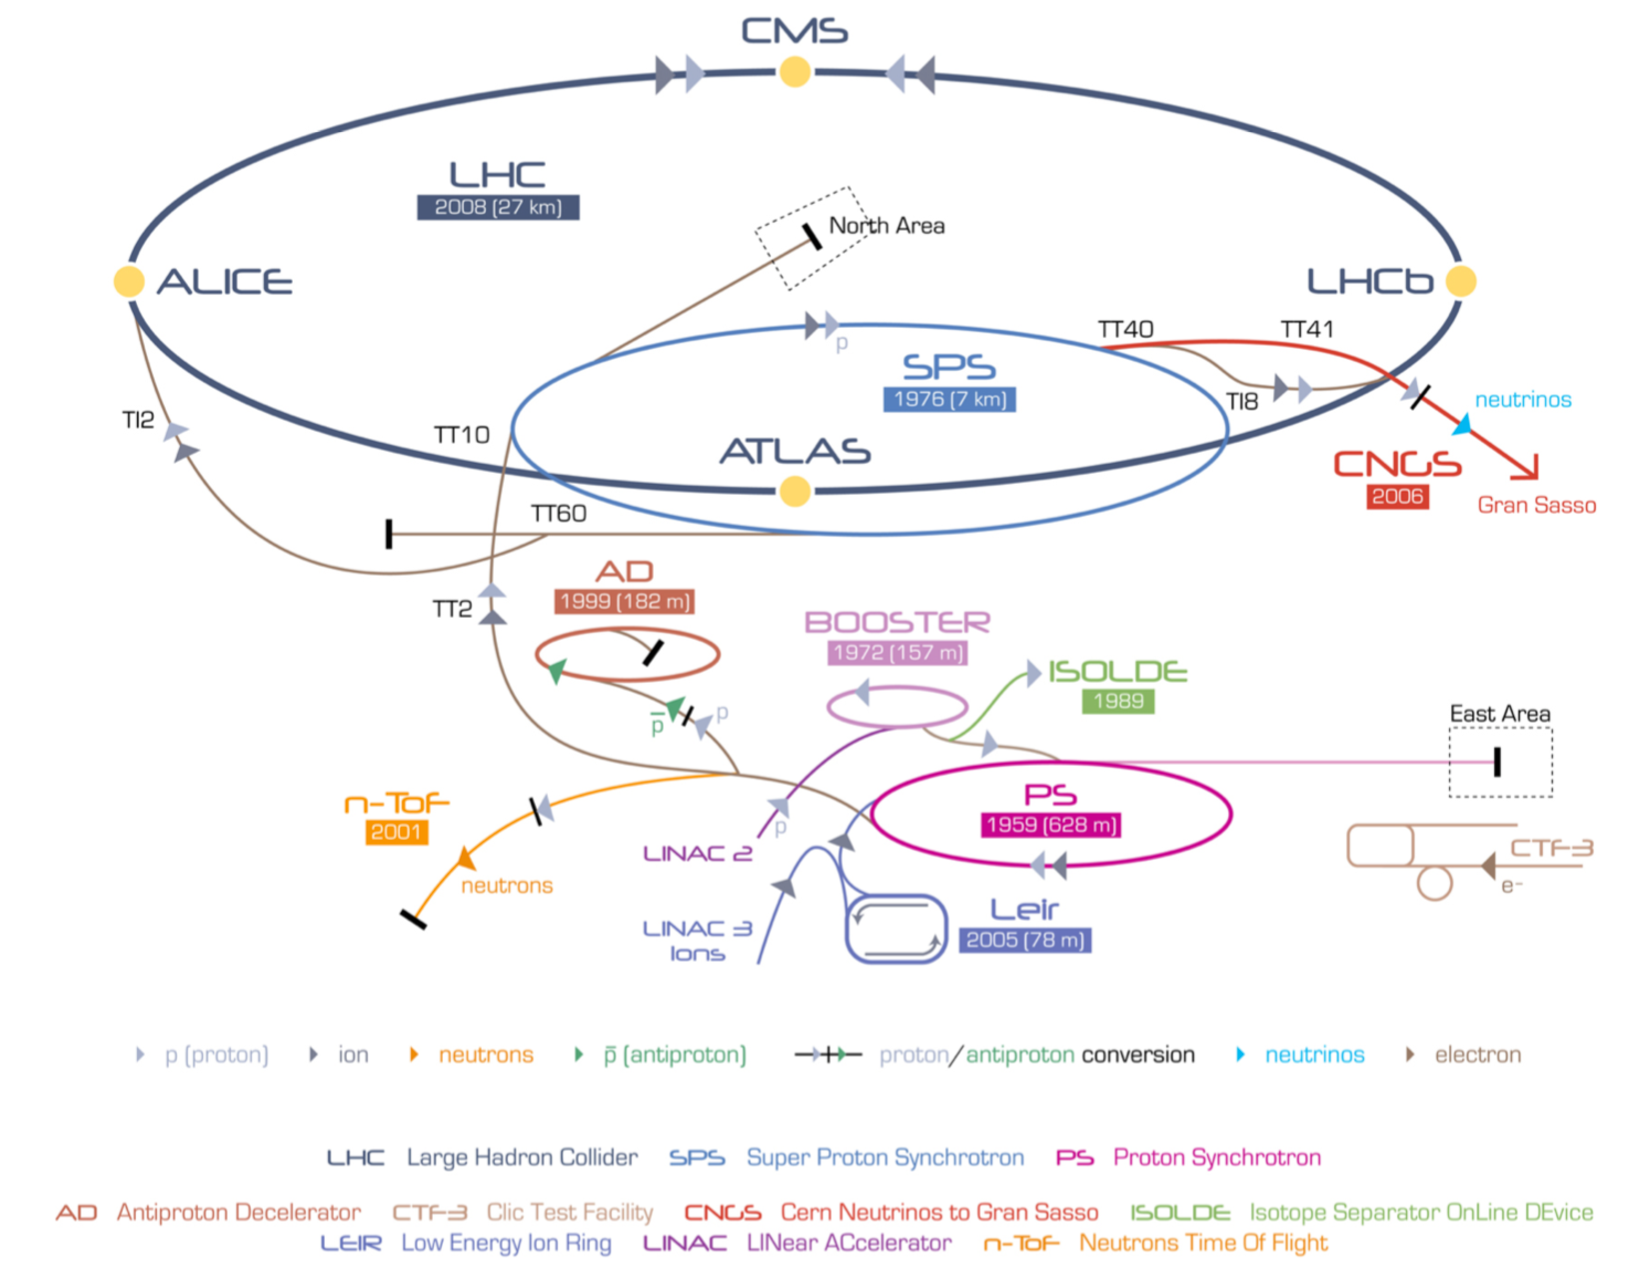
\includegraphics[width=0.75\textwidth, trim=2cm 0cm 1cm 1cm,clip]
                  {CERNaccelerators}
  \caption{The CERN experiments and accelerators.  This figure is taken
    from~\cite{cernaccel}.}
  \label{fig::CERNaccelerators}
\end{figure}

The COMPASS spectrometer is a two-stage spectrometer.  The two stages are in
series where each stage contains various tracking detectors and a muon wall
filter at the end of each stage.  Any particles that penetrate through the
active area of either of the muon wall filters are with a high probability,
muons.  Both stages also contain an electromagnetic and hadron calorimeter.  The
stages are both centered around a strong spectrometer magnet used for
determining charged particle momentum.  The first stage downstream of the target
is the large angle spectrometer (LAS) and it is centered around the SM1 magnet,
which has an integrated field of 1~Tm.  This stage detects tracks with larger
polar scattering angles approximately between 26~mrad and 160~mrad.  The second
stage is the small angle spectrometer (SAS) and it detects particle tracks
having a scattering angle between roughly 8~mrad and 45~mrad.  This stage is
centered around the SM2 magnet which has an integrated field of 4.4~Tm. \par

The left and right side of the spectrometer are referred to by the mountains
that surround the spectrometer.  When looking down the beam line, the left side
is referred to as the Jura side, which roughly corresponds to the west side.
The right side is referred to as the Saleve side, which roughly corresponds to
the east side.  A graphic of the 2015 setup is shown in
Fig~\ref{fig::compassSpec}.\par

This chapter gives an overview of the general COMPASS data taking setup and
highlights the specific features in 2015.  All the data in this thesis was
obtained with the 2015 setup.  For a more thorough review of the spectrometer
see reference~\cite{compassSpec}.  This chapter is roughly organized by how the
data taking occurs and concludes with an extra section summarizing the unique
features of the 2015 Drell-Yan data taking conditions. \par

\begin{figure}[h!t]
  \centering
  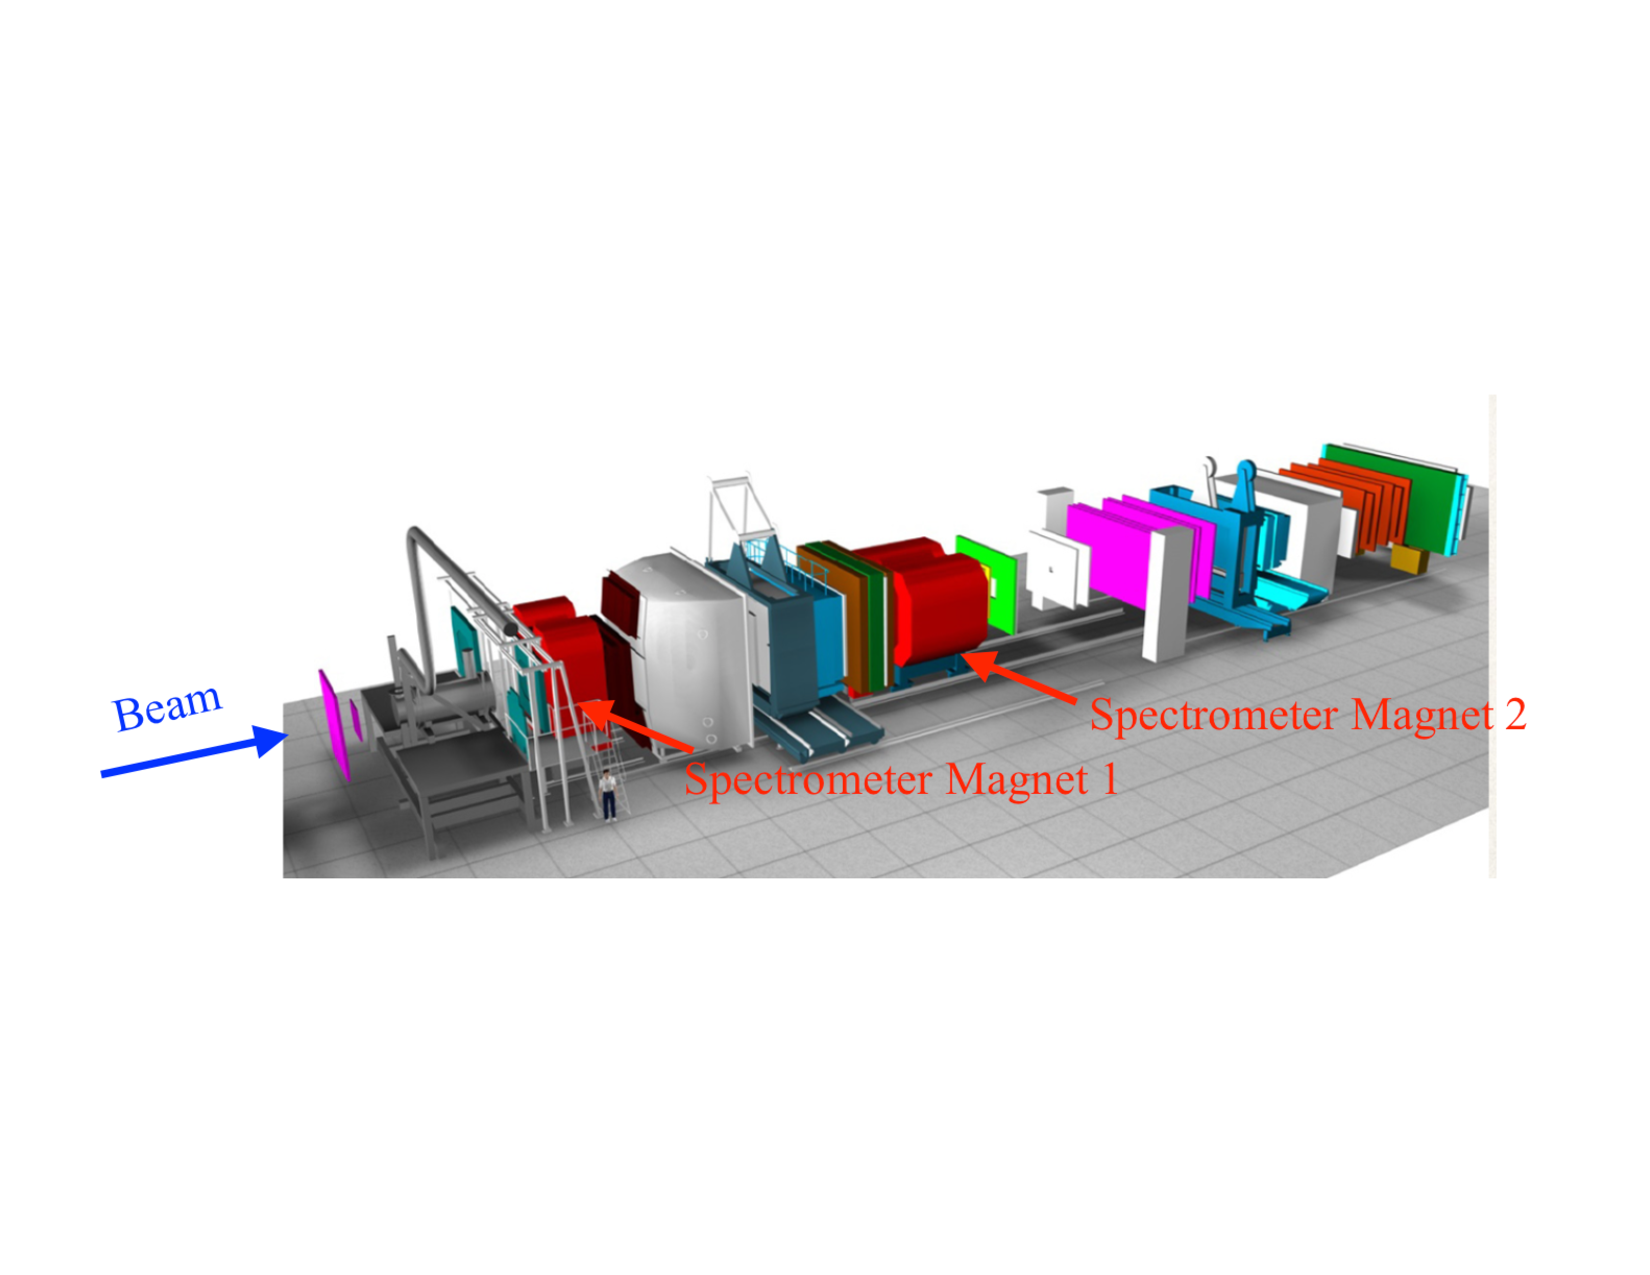
\includegraphics[width=\textwidth, trim=0.5cm 7cm 0.7cm 7cm,clip]{compassSpec}
  \caption{A schematic of the 2015 COMPASS setup.  This figure was taken
    from~\cite{compasswebpage}.}
  \label{fig::compassSpec}
\end{figure}

\section{The Beam}
The COMPASS spectrometer receives beam from the Super Proton Synchrotron along
the M2 beam line.  A schematic of the components in the M2 beam line is shown in
Fig.~\ref{fig::M2line}.  The SPS is the second largest accelerator at CERN with
a circumference of almost 7 km, which accelerates protons up to an energy of
450~GeV.  The SPS extracts beam to the famous Large Hadron Collier and as well
sends beam to various experiments in the North Area at CERN.  While the COMPASS
spectrometer is above ground, the SPS is below ground and the M2 beam line must
bend the beam from below ground to ground level. \par

There are several different beam types and energies available to COMPASS.  The
beam types used for the physics programs are a tertiary muon beam up to
190~{\gvc} and secondary hadron beam with an energy up to 280~{\gvc}.  Both of
the previous beam types can have a positive or negative charge.  As well as the
other two beam types it is also possible to have a low intensity tertiary
electron beam, mainly used for calibrations. \par

\begin{figure}[h!t]
  \centering
  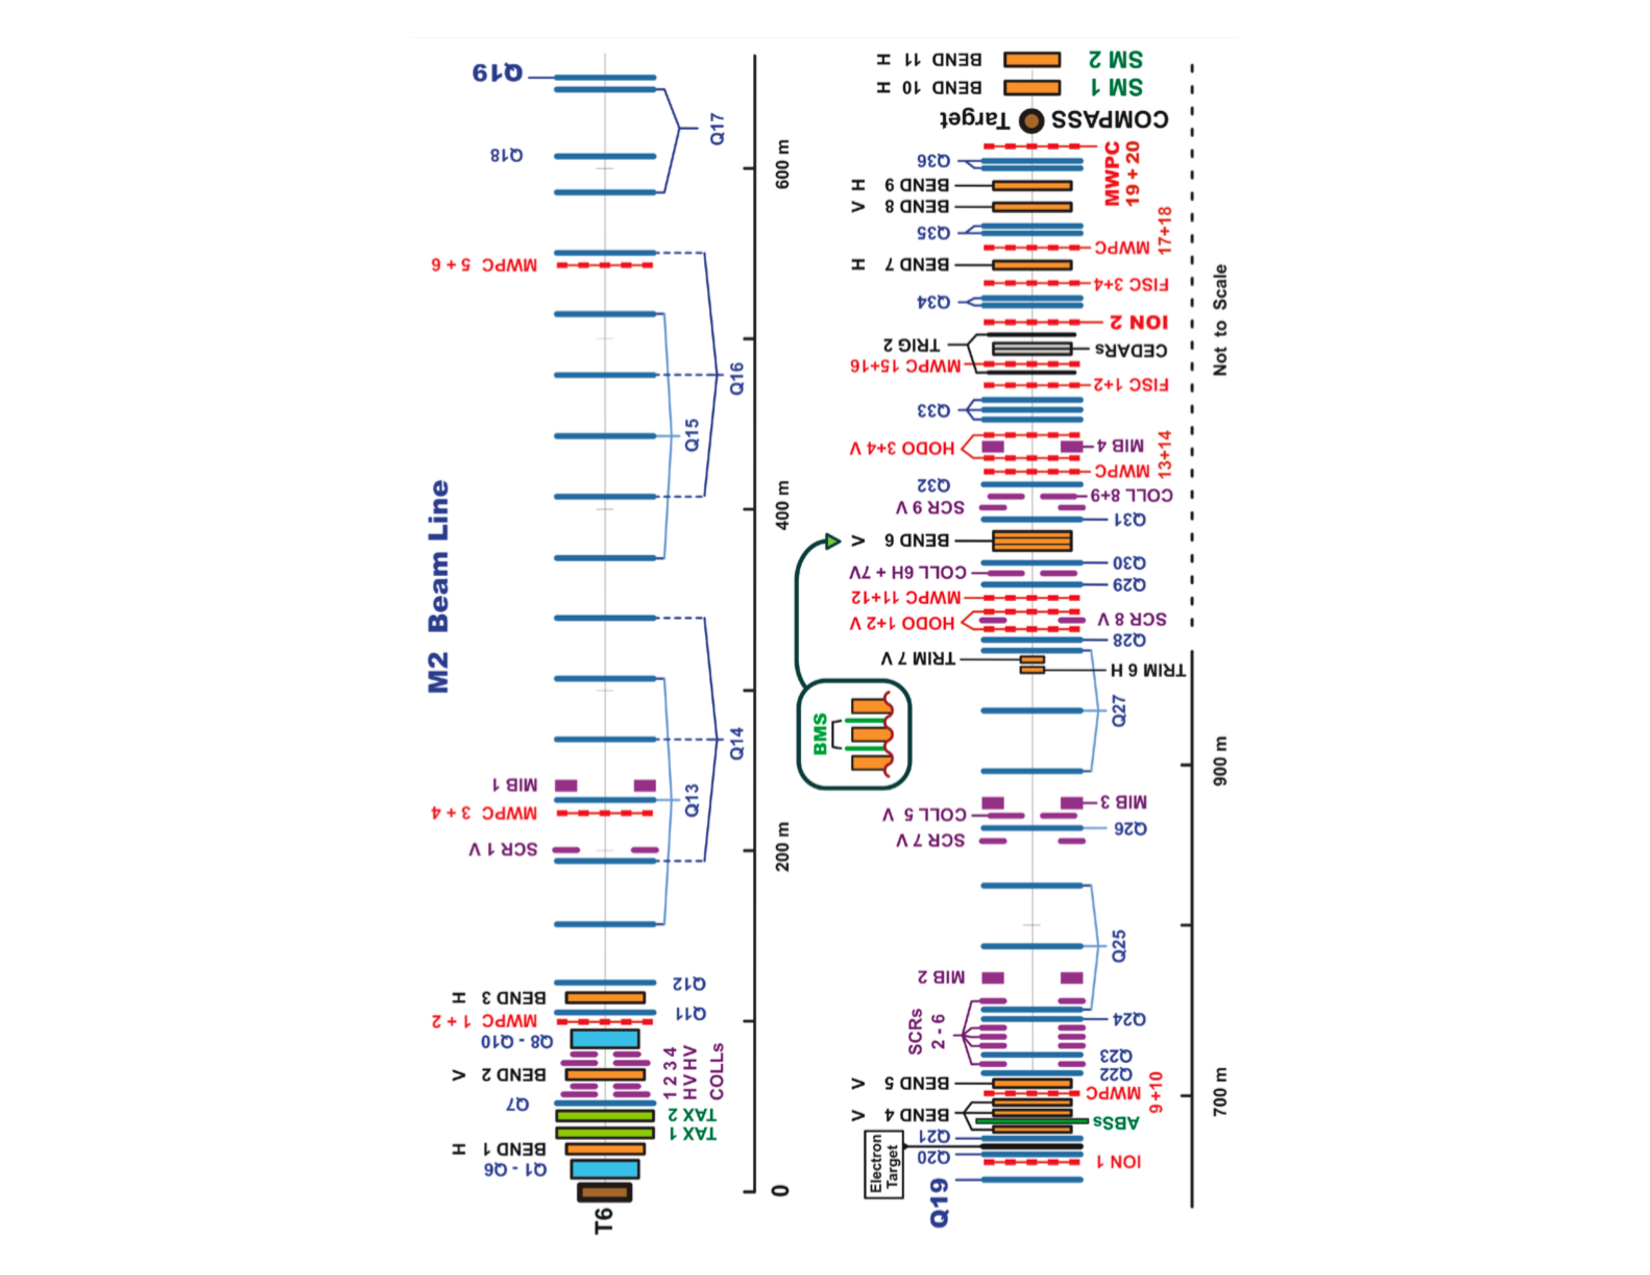
\includegraphics[width=\textwidth,trim=2cm 0cm 6cm 0cm,clip,angle=270]{M2line}
  \caption{The M2 beam line at CERN.  This image is taken
    from~\cite{ABBON201569}.}
  \label{fig::M2line}
\end{figure}

The beginning of the M2 beam line is the T6 target.  The SPS can accelerate
primary protons up to 400~{\gvc} to impinge on this T6 target, which produces a
secondary beam.  The nominal proton intensity on the T6 target is
100$\times 10^{11}$ spill$^{-1}$.  The T6 target is made of beryllium and has an
adjustable length.  The longer the T6 target the higher the secondary intensity,
where 500mm is the longest and typical target length used for physics data
taking.  The reaction of the proton beam with the T6 mainly produces secondary
protons, pions and kaons.  Following this reaction a series of dipole and
quadruple magnets select the momentum and charge of interest. \par

The SPS spill structure varies throughout the data taking year depending mainly
on the needs of the Large Hadron Colider (LHC).  In 2015, the average intensity
provided was 0.6$\times 10^8$ s$^{-1}$ and the typical spill structure was two
4.8~second spills every 36~seconds.

\subsection{Muon Beam}
The muon beam is a tertiary beam which results from a weak decay of the
secondary beam.  After the initial proton reaction on T6 the resulting secondary
particles are momentum and charge selected and sent through a 600m tunnel with
focusing and de-focusing (FODO) quadruple magnets.  In this tunnel the secondary
pions and kaons can decay as
\begin{equation}
  \pi^{-(+)} \rightarrow \mu^{-(+)} + \overline{\nu}_{\mu^-}(\nu_{\mu^+})
  \label{eqn::pionDecay}
\end{equation}
\noindent
and
\begin{equation}
  \mathrm{K}^{-(+)} \rightarrow \mu^{-(+)} +
  \overline{\nu}_{\mu^-}(\nu_{\mu^+}),
  \label{eqn::kaonDecay}
\end{equation}
\noindent
where K$^{-(+)}$ is a kaon of negative or positive charge.  At the end of the
tunnel, a series of nine 1.1~m long beryllium absorbers, referred to as the ABS
in Fig.~\ref{fig::M2line}, remove the remaining hadron component that did not
decay.  A 172~{\gvc} secondary pion beam is chosen to achieve a 160~{\gvc}
tertiary muon beam.  Due to the fact that the neutrino in the reactions
\ref{eqn::pionDecay} and \ref{eqn::kaonDecay} is always left handed, the muon
will naturally be longitudinally polarized.  For the muon momentum chosen, the
muon beam achieves a polarization of 80\%.

\subsection{Hadron Beam}
To deliver a hadron beam to COMPASS the ABS absorbers are not used.  The decayed
muons used for the tertiary muon beam have a lower momentum than the hadron beam
and are therefore removable by magnetically rejecting these lower momentum
muons.  In the case of a negative hadron beam as in 2015, the composition of the
beam is approximately 97~\% $\pi^-$, 2.5\% kaons and 0.5\%
$\overline{\mathrm{p}}$. The 2015 Drell-Yan data taking was performed with a
190~{\gvc} hadron beam. \par

\subsection{Additional Beam Line Components} \label{sec::addBeam}
After the decay tunnel the beam is bent upwards along another FODO tunnel.  The
lenght of this tunnel is 250m and reaches the surface level approximately 100m
before the COMPASS target.  A series of three dipole magnets, called bend 6,
then bend the beam to a horizontal position aimed at the COMPASS target.  Both
upstream and downstream of bend 6, there are three tracking detectors
(BM01-BM06) that make up the Beam Momentum Station (BMS).  The BMS is the
upstream most component of the COMPASS spectrometer.  It is able to determine
the beam momentum to better than 1\% of the beam momentum with an efficiency of
approximately 93\%.  Bend 6 and the BMS are shown schematically in
Fig.~\ref{fig::BeamLine1}. \par

\begin{figure}[h!t]
  \centering
  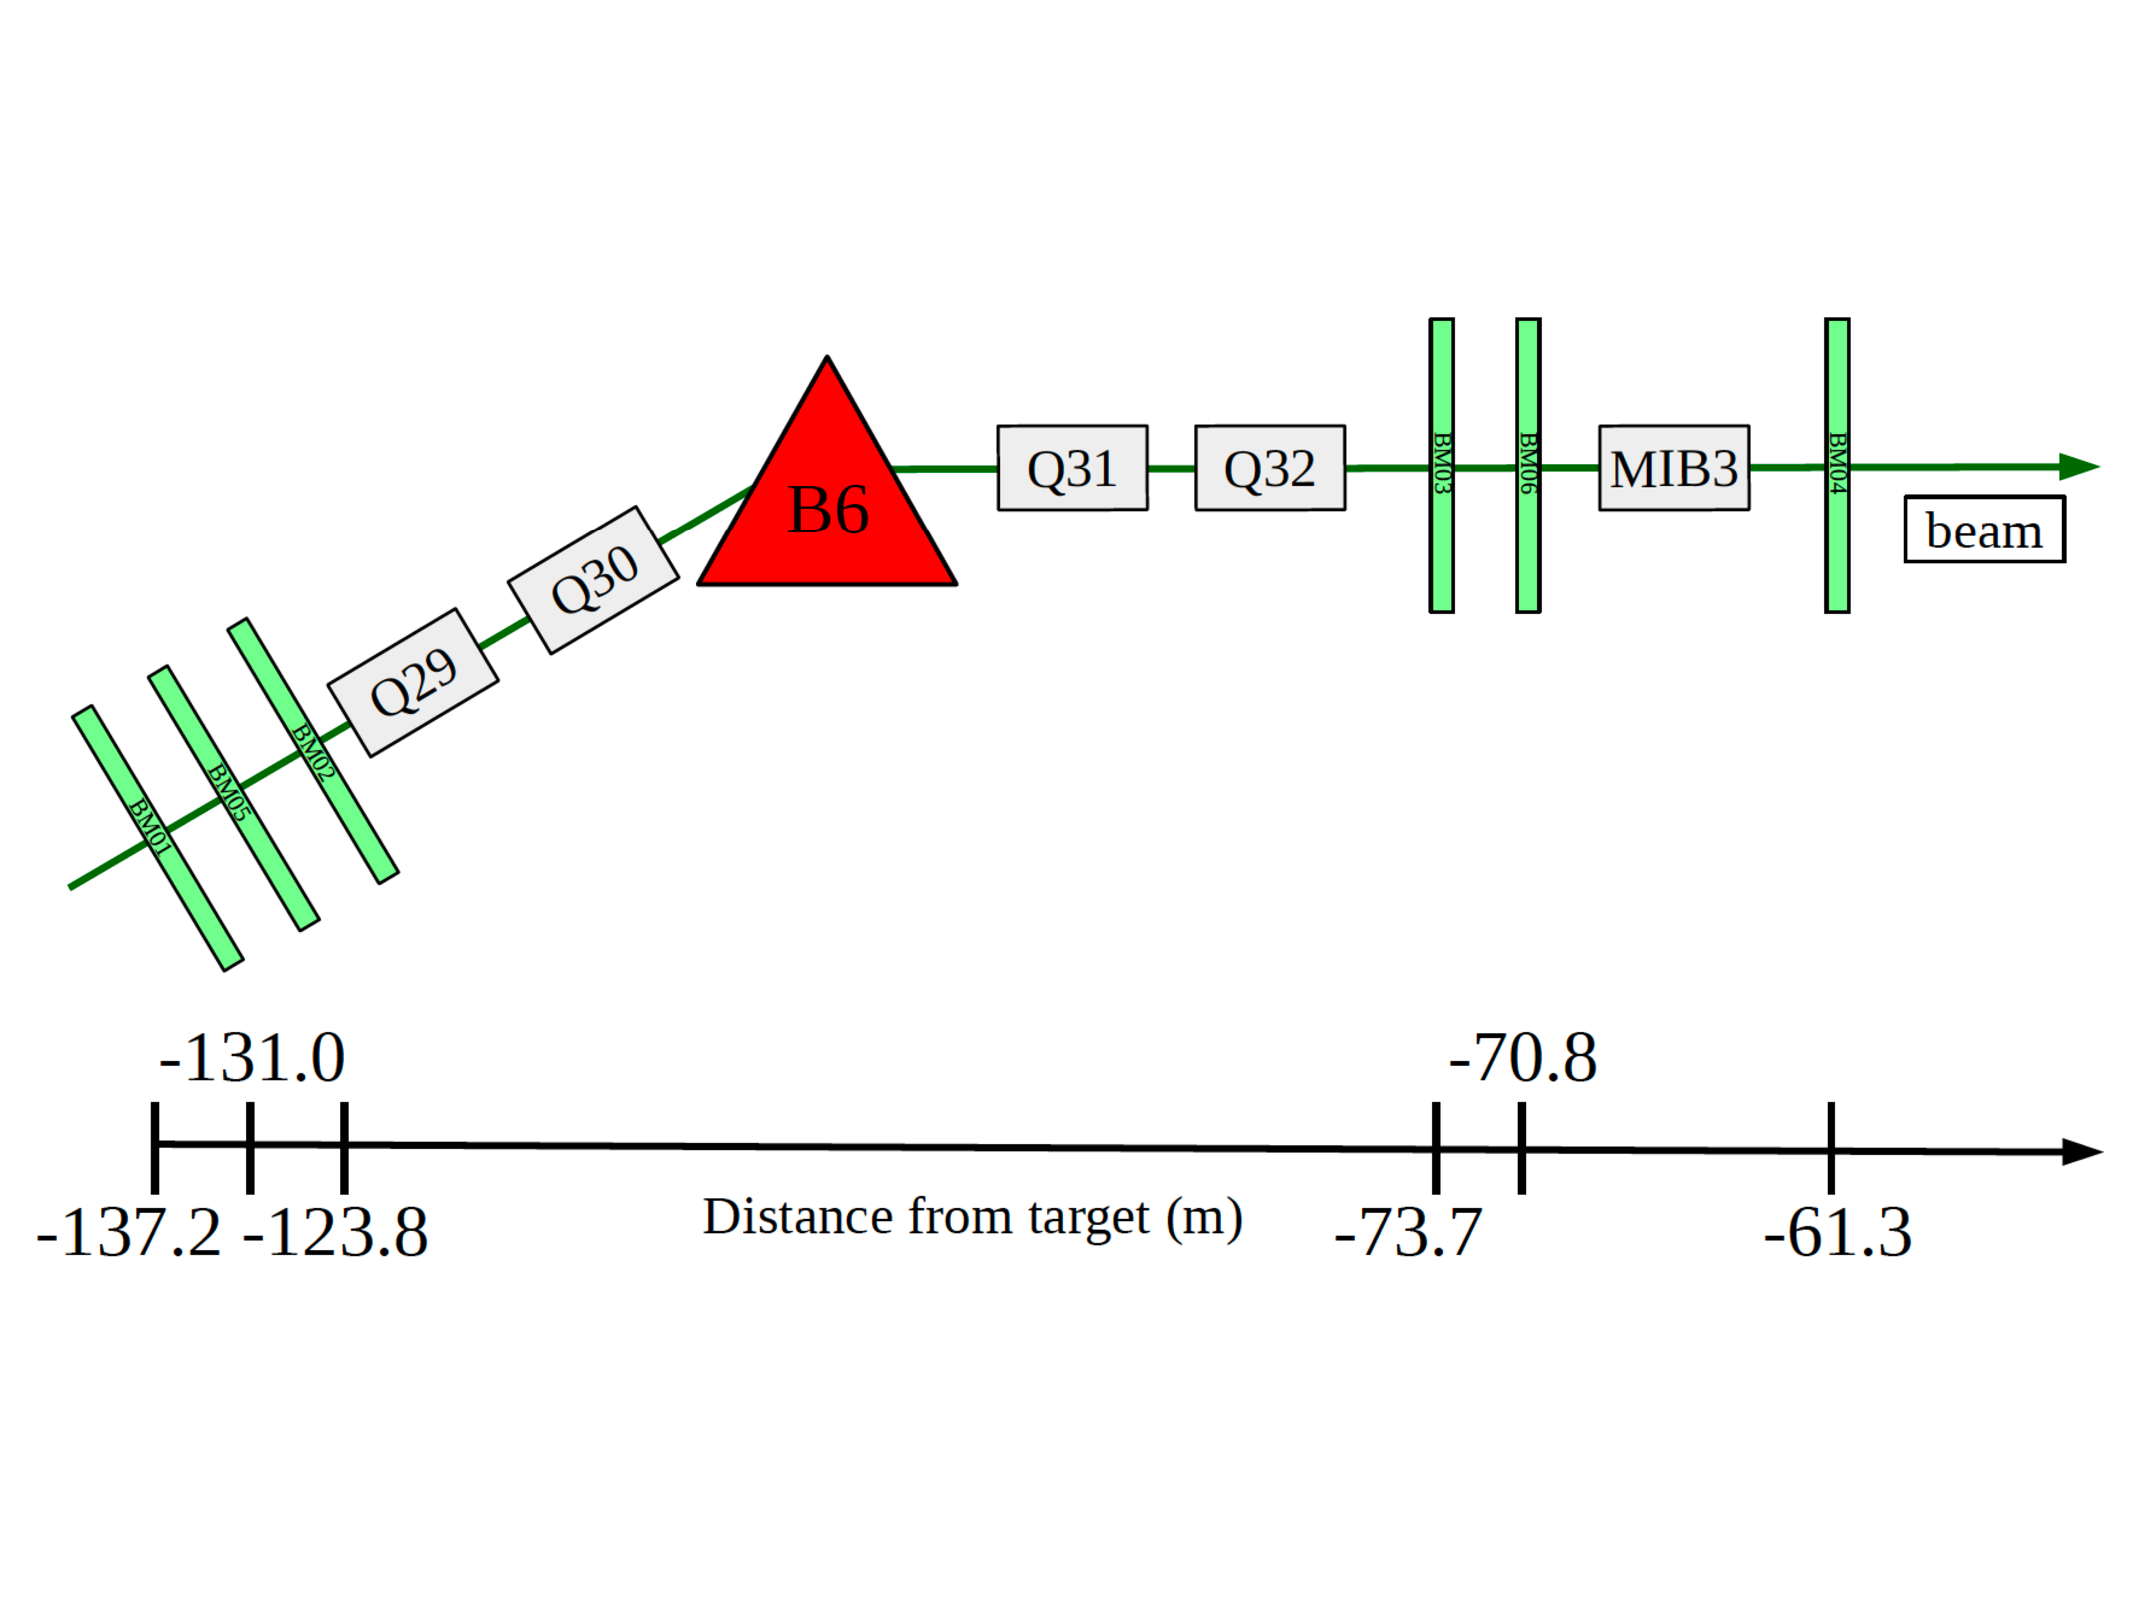
\includegraphics[width=0.8\textwidth]{BeamLine1}
  \caption{Bending the beam to a horizontal position.  The BMS detectors (green
    boxes) are upstream and downstream of the bend 6 magnet (red triangle
    labeled B6).  This image was taken from~\cite{compassSpec}.}
  \label{fig::BeamLine1}
\end{figure}

During the 2015 Drell-Yan setup the $\pi^-$ beam intensity was too high for the
BMS station to work properly.  For this reason, special low intensity,
approximately 10$^6$ s$^{-1}$, $\pi^-$ beams were used in 2014 to determine the
momentum distribution during Drell-Yan data taking.  The beam momentum
distribution is shown in Fig.~\ref{fig::BeamMomBMS}, where the average momentum
is 190.9~{\gvc} with a spread of $\pm$ 3.2~{\gvc}. \par

\begin{figure}[h!t]
  \centering
  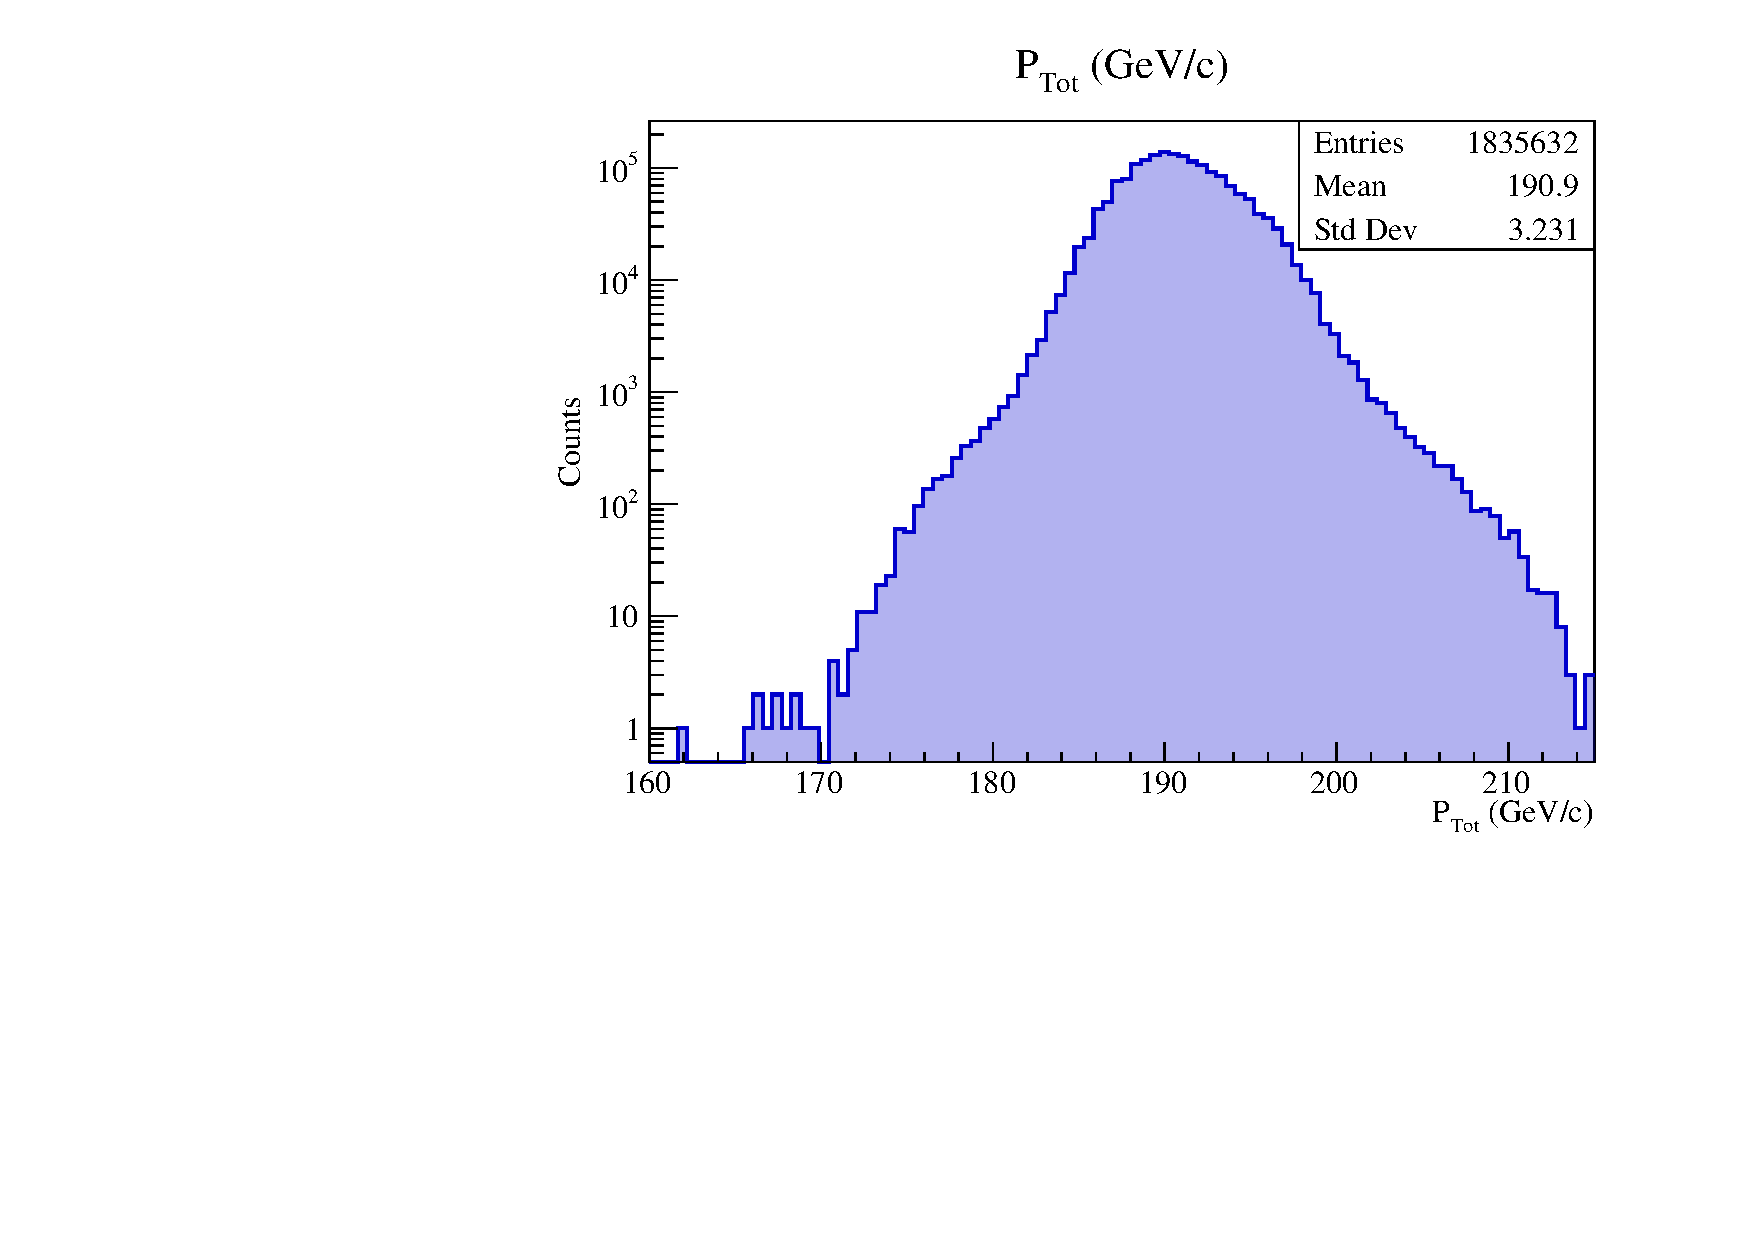
\includegraphics[width=0.5\textwidth]{BeamMomBMS}
  \caption{The momentum distribution of the $\pi^-$ beam, determined during
    dedicated low intensity beam conditions.  This figure was taken
    from~\cite{COMPbeamProp}.}
  \label{fig::BeamMomBMS}
\end{figure}

Approximately 30~m upstream of the target are to two Cherenkov counter (CEDAR)
detectors.  As the hadron beam has contamination from several components these
CEDARs can be used to distinguish between the different components.  The CEDARs
general principle of operation is that two particles with the same momentum but
different mass will emit Cherenkov radiation at different angles relative to
their momentum.  When a particle is traveling faster than the speed of light in
a given medium, it emits Cherenkov radiation in a cone centered along its
momentum axis.  The faster the particle is traveling, the narrower the angle of
the Cherenkov light cone.  A schematic of the CEDAR operating principle is shown
in Fig.~\ref{fig::cedars}.  In 2015 the CEDARs were measured to be largely
inefficient due to the high beam intensity and are not used for the analysis of
this thesis.

\begin{figure}[h!t]
  \centering
  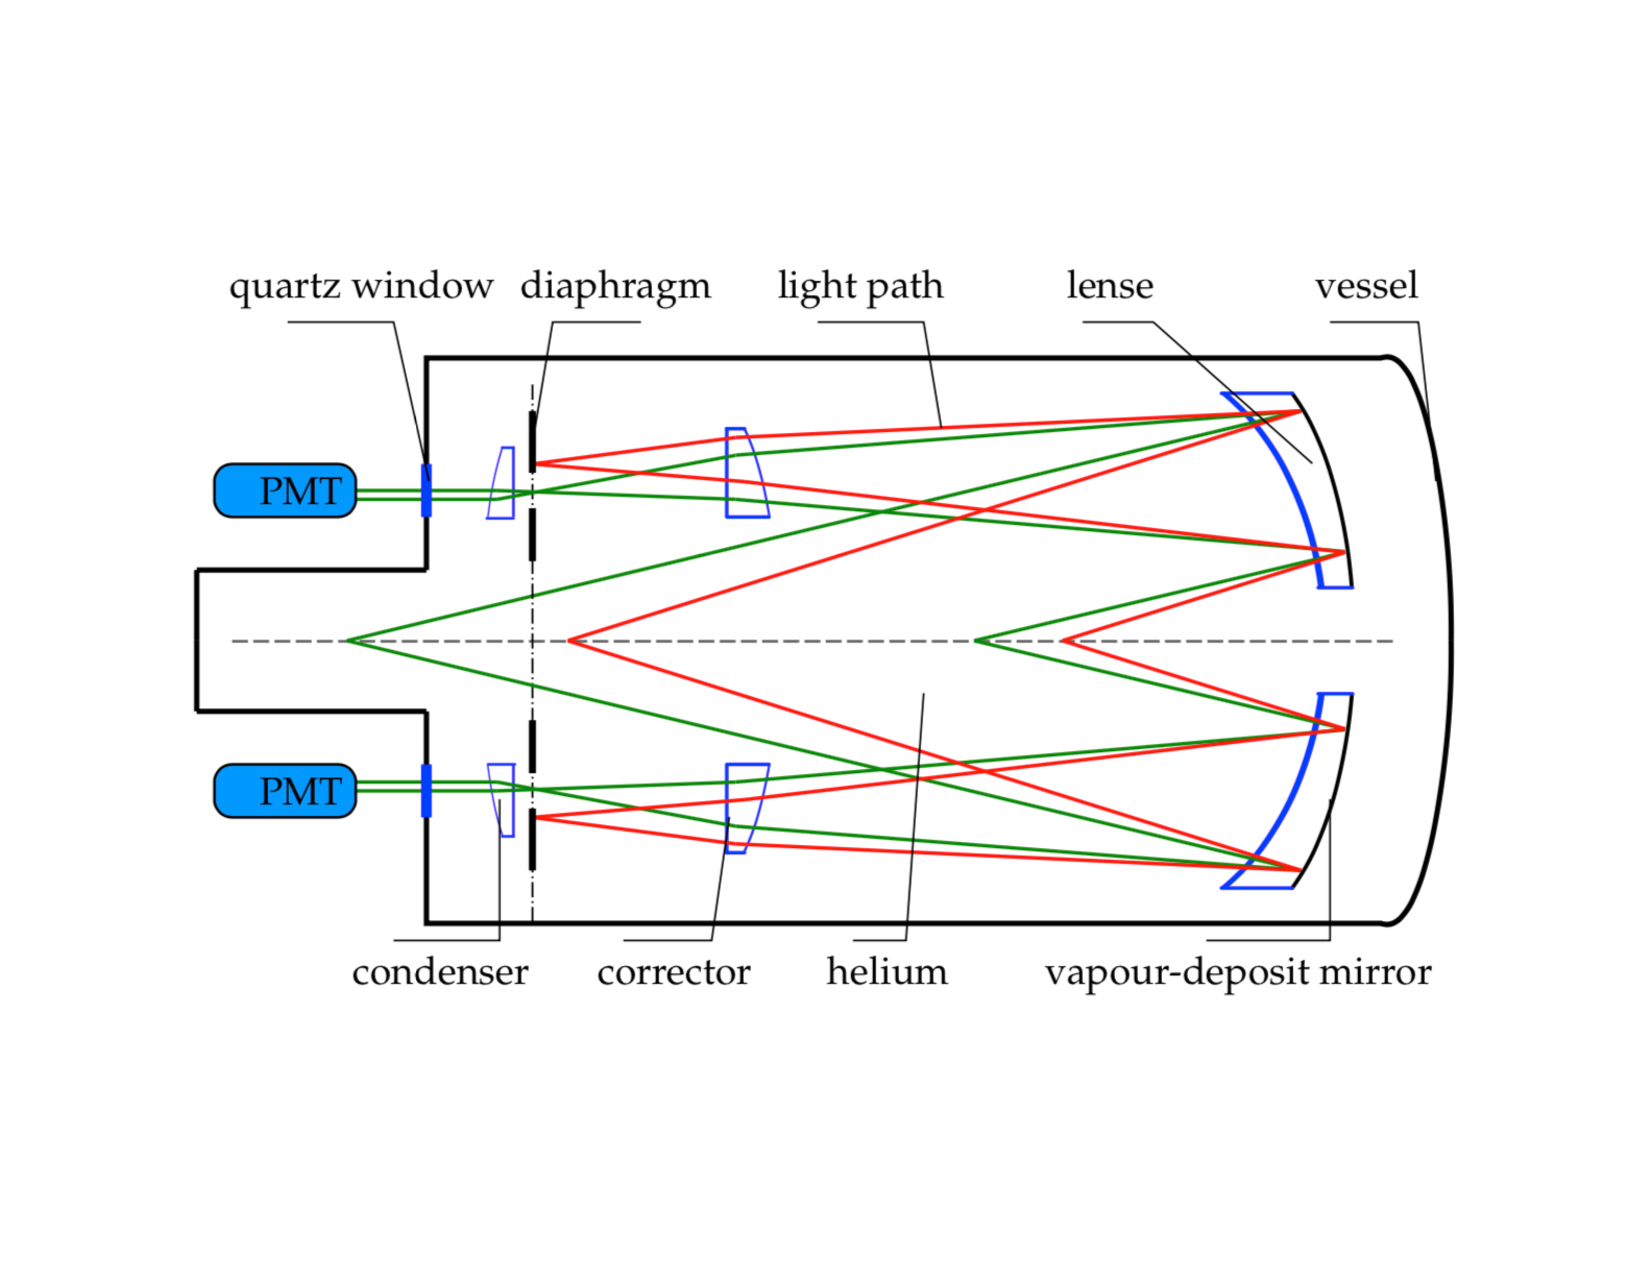
\includegraphics[width=0.5\textwidth,trim=2cm 4cm 2cm 4cm,clip]{cedars}
  \caption{Light lines emitted inside CEDARs at COMPASS.  The red(green) lines
    correspond to Cherenkov light emitted from a particle lower(higher)
    momentum.  This image is taken from~\cite{ABBON201569}.}
  \label{fig::cedars}
\end{figure}

For years with a transversely polarized target, such as 2015, a chicane system
of dipole magnets is setup in front of the target.  The chicane first bends the
beam away from the beam line and then back to the target such that the beam hits
the target at an angle.  A chicane magnet setup is used because a beam hitting
the target without any angle would then be deflected from the target magnet to
the left or right of the spectrometer.  For this reason the chicane gives the
beam an angle before hitting the target such that the non-interacting beam exits
the target traveling straight towards the spectrometer.


\section{The Polarized Target} \label{sec::polTarget}
The polarized target at COMPASS is the most complicated and essential component
of the spectrometer.  It is located upstream of the tracking detectors and
spectrometer magnets and downstream of the beam telescope detectors, described
in section~\ref{sec::tracking}.  The target consists of two or three cylindrical
cells.  The possible materials are either solid state ammonia (NH$_3$) or
deuterated lithium ($^6$LiD) or liquid
hydrogen~\cite{Matousek:2017rvj,Koivuniemi:2015uyw,GenkiPolTarget}.
Fig.~\ref{fig::PT} shows a schematic of the target.  \par

\begin{figure}[h!t]
  \centering
  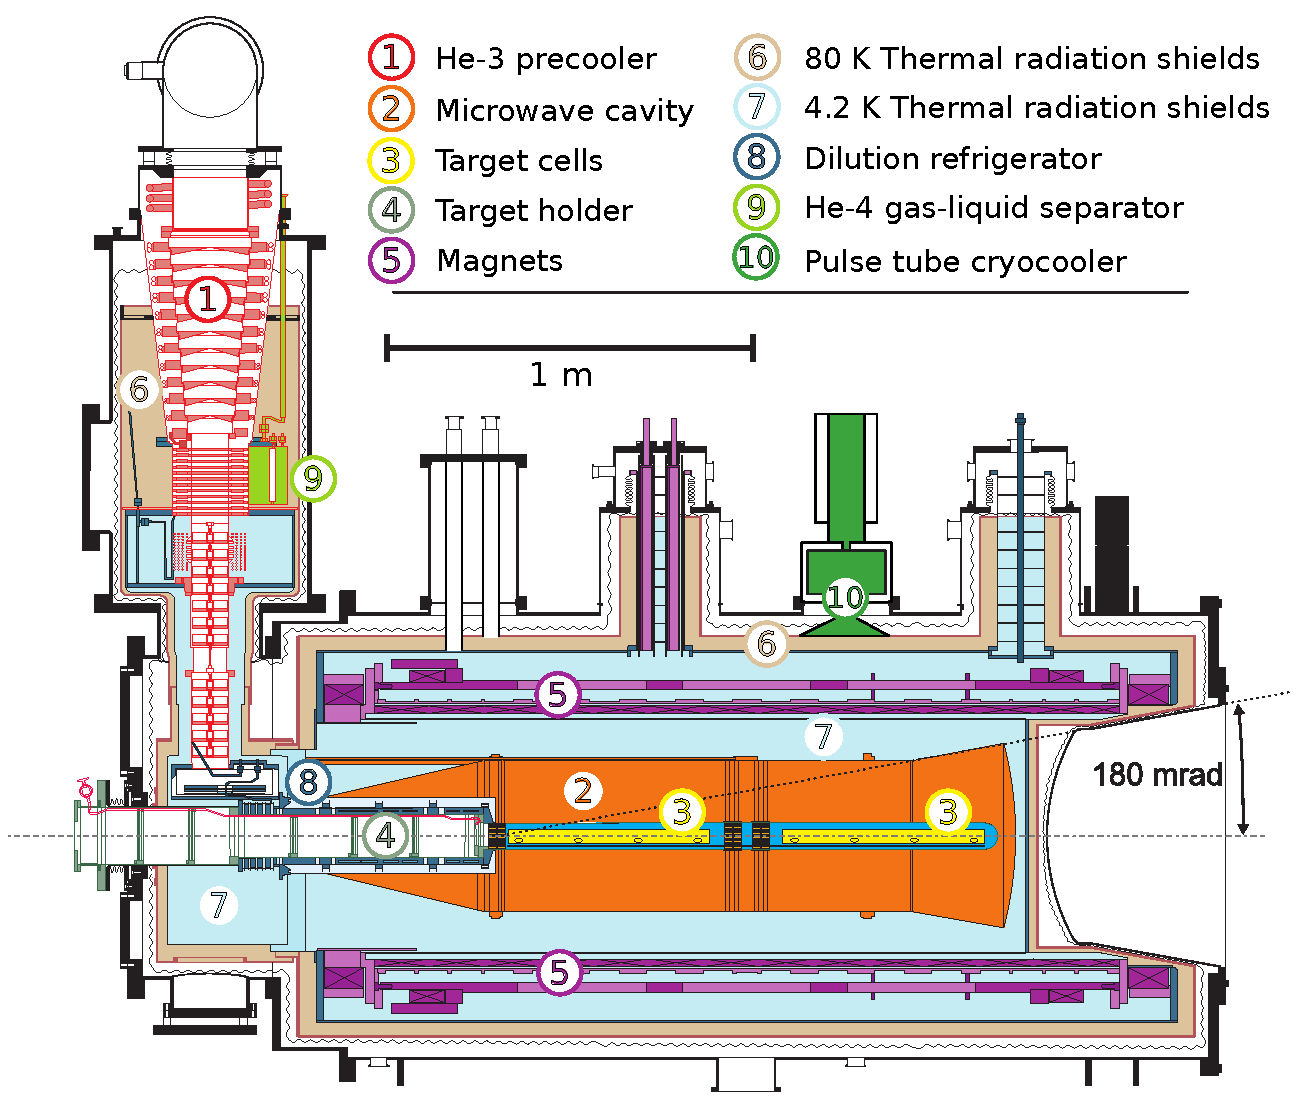
\includegraphics[width=0.8\textwidth]{PT}
  \caption{The polarized target at COMPASS.  This image taken
    from~\cite{Matousek:2017rvj}.}
  \label{fig::PT}
\end{figure}

Surrounding the cylindrical cells is a longitudinal super-conducting magnet
capable of reaching a magnetic field of 2.5~T.  This longitudinal magnet
polarizes the protons or deuterons in the target material parallel or
anti-parallel to the spectrometer axis.  The target polarization is
maintained by keeping the target in a liquid helium bath of approximately 60~mK.
This is called frozen spin mode where the temperature is maintained by a
dilution refrigerator. \par

The target is polarized through the dynamic nuclear polarization (DNP)
method~\cite{DNPmethod}.  This process works by first polarizing electrons in
the target with the longitudinal magnet.  With a high probability, the target
electrons are all polarized in the same longitudinal direction for each target
cells.  Due to their much lower mass, electrons have a larger magnetic moment
and therefore can be polarized at a much faster rate than protons or neutrons.
At the same time the electrons are being longitudinally polarized, microwave
electromagnetic radiation is sent through each target cell.  For atoms that have
a nuclear spin it is then possible to absorb a microwave and go to an excited
state with the electron spin anti-parallel to the magnet field direction and the
nuclear spin either parallel or anti-parallel to the magnet field direction
depending on the microwave frequency.  To ensure only one frequency enters each
target cell, there is a microwave stopper between each target cell.  The
electron with the anti-aligned spin will then quickly have its spin realigned
while the nucleon will take much longer to lose its polarization due to its
smaller magnetic moment.  This process can continue in this way resulting in a
net nuclear polarization.  Using the DNP method the target proton or deuteron
can achieve a polarization of approximately 90\% in three days. \par

The target also includes a 0.63~T transverse dipole magnet to change from
longitudinal to transverse polarization.  The target must first be
longitudinally polarized before the transverse target magnet can change the
polarization direction.  Once the target is transversely polarized, the target
polarization can no longer be increased as microwaves can no longer shine on the
target in the polarization direction.  Therefore the polarization will decrease
exponentially.  In 2015 the target was polarized for about half a day between
data taking sub-periods and achieved an average polarization of 0.73\%,
including the effects of exponential polarization loss with time.  The
relaxation time of the target polarization was about 1000 hours in 2015. \par

The target polarization was measured with 10 NMR coils while the target cells
were longitudinal polarized.  In the 2015, each target cell had the most
upstream and downstream coils in the center of the target cell and the other
three coils on the outside perimeter as is shown in Fig.~\ref{fig::targCells}.
Due to the fact that the polarization can only be measured with the longitudinal
magnet on, the polarization is only measure at the start and finish of a
transversely polarized data taking.  The intermediate polarization is then
determined by exponential interpolating between these two times.

\begin{figure}[h!t]
  \centering
  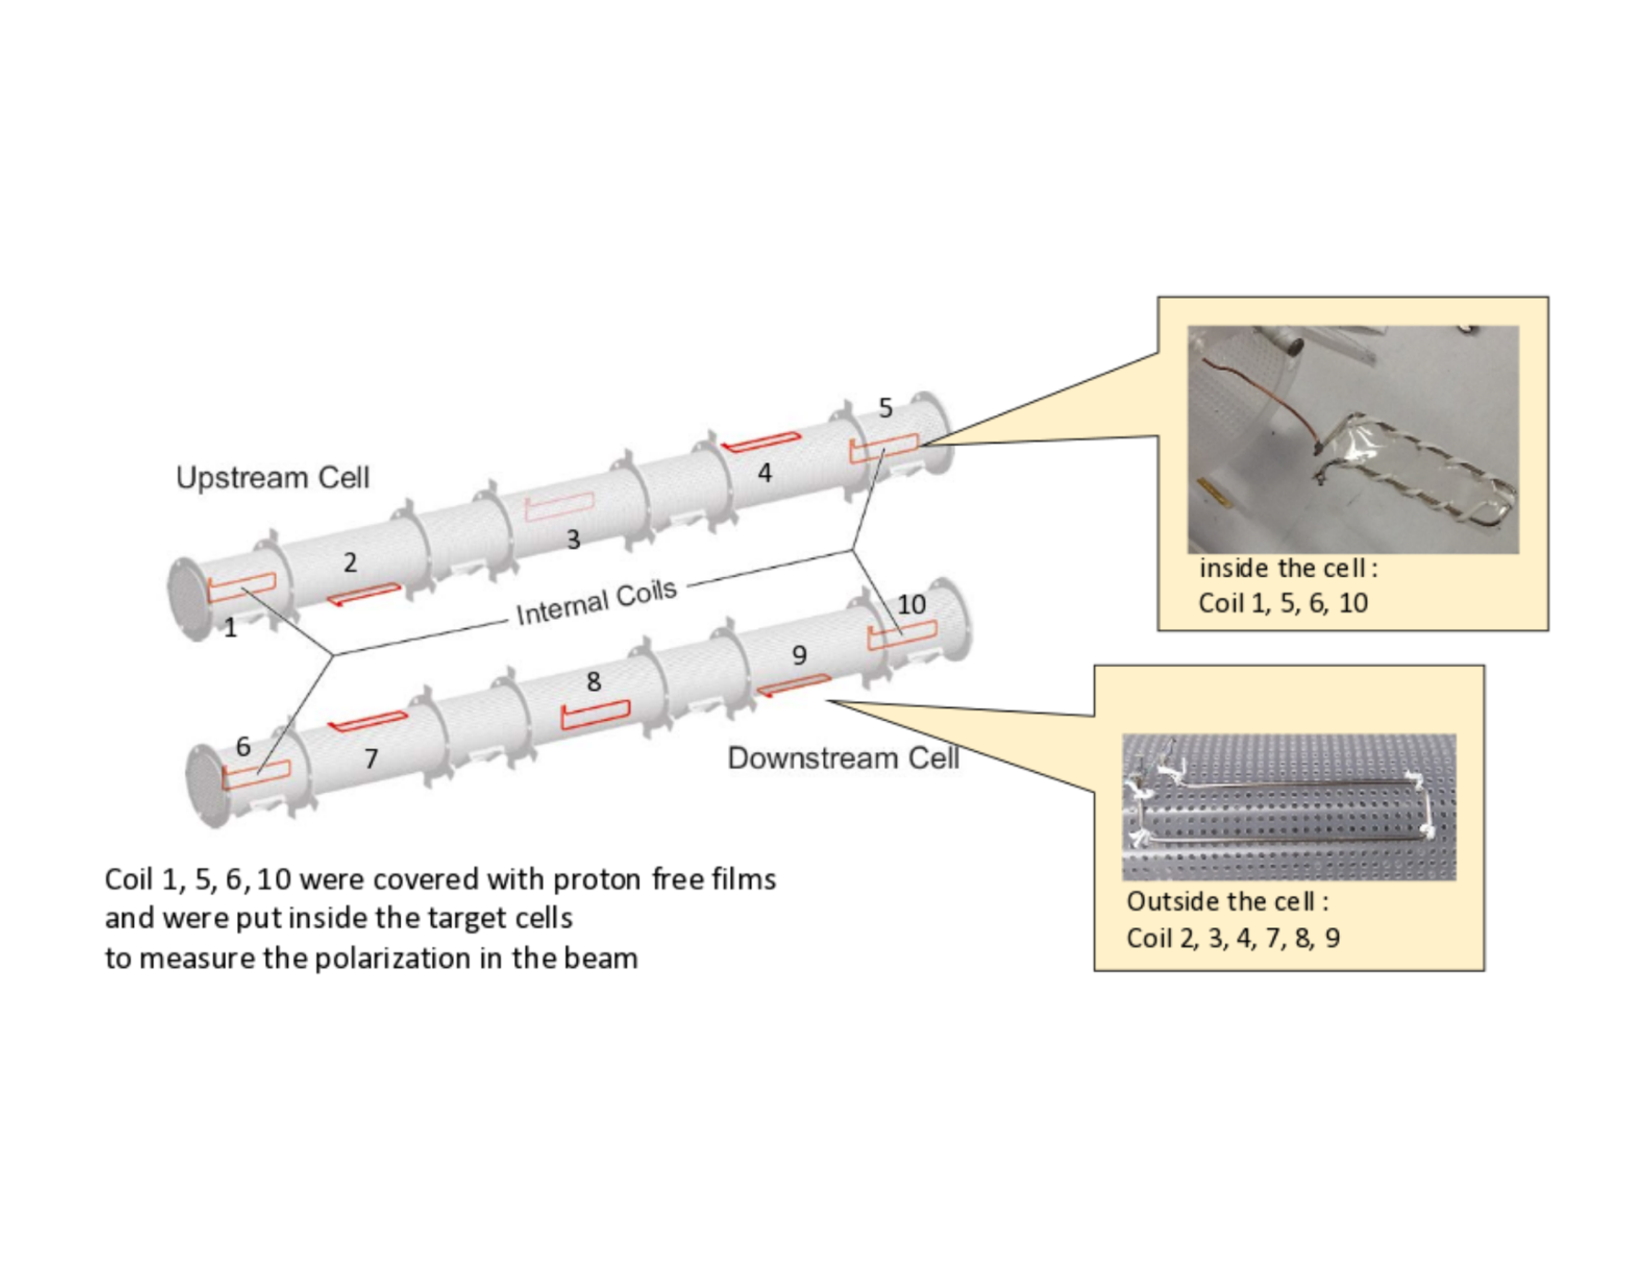
\includegraphics[width=0.8\textwidth]{targCells}
  \caption{The empty polarized target cells side by side along with their NMR
    coil positions.  This image taken from~\cite{polTargCells}.}
  \label{fig::targCells}
\end{figure}

In 2015 the setup was two transversely polarized target cells of 55~cm length
and 2~cm in radius.  The cells were separated by 20~cm and polarized in opposite
directions.  The polarization of the target cells was flipped ever two weeks of
data taking to reduce systematic effects from luminosity and geometrical
spectrometer acceptance.  Due to the fact that the beam needs to be precisely
steered onto the target and that the chicane magnets upstream of the target are
setup for only one transverse target magnet direction, the transverse target
magnet only pointed downward in 2015.  To achieve a polarization flip the target
polarization had to therefore be rotated back to the longitudinal direction and
the input microwaves had to be changed to achieve the desired polarization
direction. \par

The target material in 2015 was solid state NH$_3$.  The protons in the three
hydrogen atoms were the only nucleons with nuclear spin and therefore only some
fraction of the target was able to be polarized.  The fraction of polarized
nucleons to total nucleons is called the dilution factor.  Counting the ratio of
unpolarized nitrogen nucleons to polarized hydrogen, one would expect the
dilution to be 3/17.  However to get a more accurate determination of the
dilution factor the follow calculation was used

\begin{equation}
  f = \frac{n_H\sigma^{DY}_{\pi^-H}}
  {n_h\sigma^{DY}_{\pi^-H} + \sum_A n_A\sigma^{DY}_{\pi^-A}},
  \label{equ::dilution}
\end{equation}
where $f$ is the dilution factor, $n_H$ is the number of hydrogen atoms in
NH$_3$, $n_A$ is the number of other nucleons in NH$_3$, and
$\sigma^{DY}_{\pi^-H}$ and $\sigma^{DY}_{\pi^-A}$ are the Drell-Yan
cross-sections for pion-hydrogen scattering and pion-nucleon scattering
respectively.  The cross-sections were determined using a parton-level
Monte-Carlo program MCFM~\cite{MCFM}.  The dilution factor was also further
scaled down by studies of reconstruction migration between target cells.  The
average dilution factor in 2015 was determined to 0.18 in the invariant mass
range of 4.3{\gvcs} to 8.5{\gvcs}.


\section{Tracking Detectors} \label{sec::tracking}
To determine when and where a reaction occurs in the polarized target, tracking
detectors are able to position the products of the reaction.  The goal of the
tracking detectors is to determine a point in space where a particle traversed.
The COMPASS tracking detectors attempt to do this for a wide range of angles,
momenta and at different rates.  For these reasons there are several planar
tracking technologies used at COMPASS that can be divided into three
categories: very small angle trackers, small angle trackers and large area
trackers.  As the name suggests, very small angle trackers measure tracks with
small angle deflections from the beam axis which are essentially beam particles.
The small area trackers measure particle tracks with low but non-zero scattering
polar angle and have small central dead zones.  The large area trackers are
several meters in height and width and measure the largest deflection angles up
to 180~mrad. \par

All of these trackers are split into stations.  Each station corresponds to
several detectors planes at roughly the same z-position along the beam line.
Each station measures a track position in one or more orientation while most
measure tracks in three or more orientations.  The coordinate orientations
measured are the X and Y coordinates, which are the horizontal and vertical
directions respectively, and as well the U and V coordinates which are rotated
at different angles with respect the X and Y coordinates. \par

\subsection{Very Small Angle Trackers}
The very small angle trackers extend up to 3~cm away from the beam axis.  This
is the region with the highest number of particles and therefore these
detectors must be able to handle the highest rates up to 5x10$^7$~Hz.  The two
detector types that make up the very small angle trackers are either
scintillating fiber detectors (SciFi) or silicon microstrip detectors.  These
two detector types are complementary to each other as the former have very good
timing resolution, while the latter have very good spacial resolution. \par

There are three silicon stations possible at COMPASS.  These stations have
active detecting areas of 5x7~cm$^2$.  The spacial resolution of these detectors
is nominally 10~$\mu$m and the timing resolution is nominally 2.5~ns.  For the
2015 setup, the beam intensity was too high for the silicon detectors to operate
and therefore these detectors were not used. \par

There are 10 SciFi stations available at COMPASS.  The active areas vary from
3.9x3.9~cm$^2$ to 12.3x12.3~cm$^2$ planar areas.  As well the detection fiber
diameters vary between detectors with the different diameters used at COMPASS
being 0.5~nm, 0.75~nm and 1~nm.  Several fibers are bundled together to
determine a strip hit position and the resulting nominal spacial resolutions are
130~$\mu$m, 170~$\mu$m and 210~$\mu$m respectively.  The nominal timing
resolution of these detectors is about 400~ps.  In 2015 three SciFi stations
made up the beam telescope and were placed upstream of the target to measure the
beam trajectory and timing information.  A fourth SciFi station was place in the
LAS section of the spectrometer. \par

\subsection{Small Angle Trackers} \label{sec::SAT}
The small angle trackers detect particles with non-zero defection angles. These
detectors have medium size active areas compared to the very small angle
trackers and the large angle trackers.  They cover 5~cm to 40~cm from the beam
axis where the rate drops to approximate 10$^5$~Hz, two orders of magnitude
lower than the rates the very small angle trackers receive.  At COMPASS there
are two types of small area tracking detectors: micromesh gaseous structure
(micromegas) and gas electron multipliers (GEMs). \par

There are three micromega stations at COMPASS.  All three stations are located
sequentially after each other between the target and the first spectrometer
magnet.  As well all three detectors measure four coordinate projections and
have an active area of 40x40~cm$^2$ with a 5~cm diameter dead zone.  The
micromegas operate by having a conversion region and a smaller amplification
region.  An ionized particle produced in the conversion region will drift
through an electric field of around 3.2~kV/cm to the amplification region where
the electric field is around 50~kV/cm.  The electric field is too small for
amplification in the conversion region but as the name suggest the electric
field is high enough to amplify the signal in the amplification region.  The
amplified signal is then read out on strips.  The conversion and amplification
regions are separated by a metallic micromesh material.  The electrons pass
through the micromesh without resistance and are not rimmed out.  The micromegas
have good spacial resolution because the thickness of the amplification region
is only 100~$\mu$m, small enough to prevent much transverse spreading of the
electron avalanche between strips.  The separation of the larger conversion
region from the smaller amplification region with the micromesh prevents
electric field lines from being distorted in the conversion region and therefore
prevents the primary electrons from drifting slower in the conversion region.
This allows micromegas to operate at a higher rate than would be possible
otherwise.  This principle of operation is illustrated in
Fig.~\ref{fig::MicroMega}.  The strips in the central part of the detector are
360~$\mu$m corresponding to a position resolution of about 100~$\mu$m and the
strips in the outer region are 460~$\mu$m corresponding to a resolution of about
120~$\mu$m.  The nominal timing resolution is 9~ns.  In 2015 the micromegas were
upgraded to include a pixelized section covering much of the dead zone
area. \par

\begin{figure}[h!t]
  \centering
  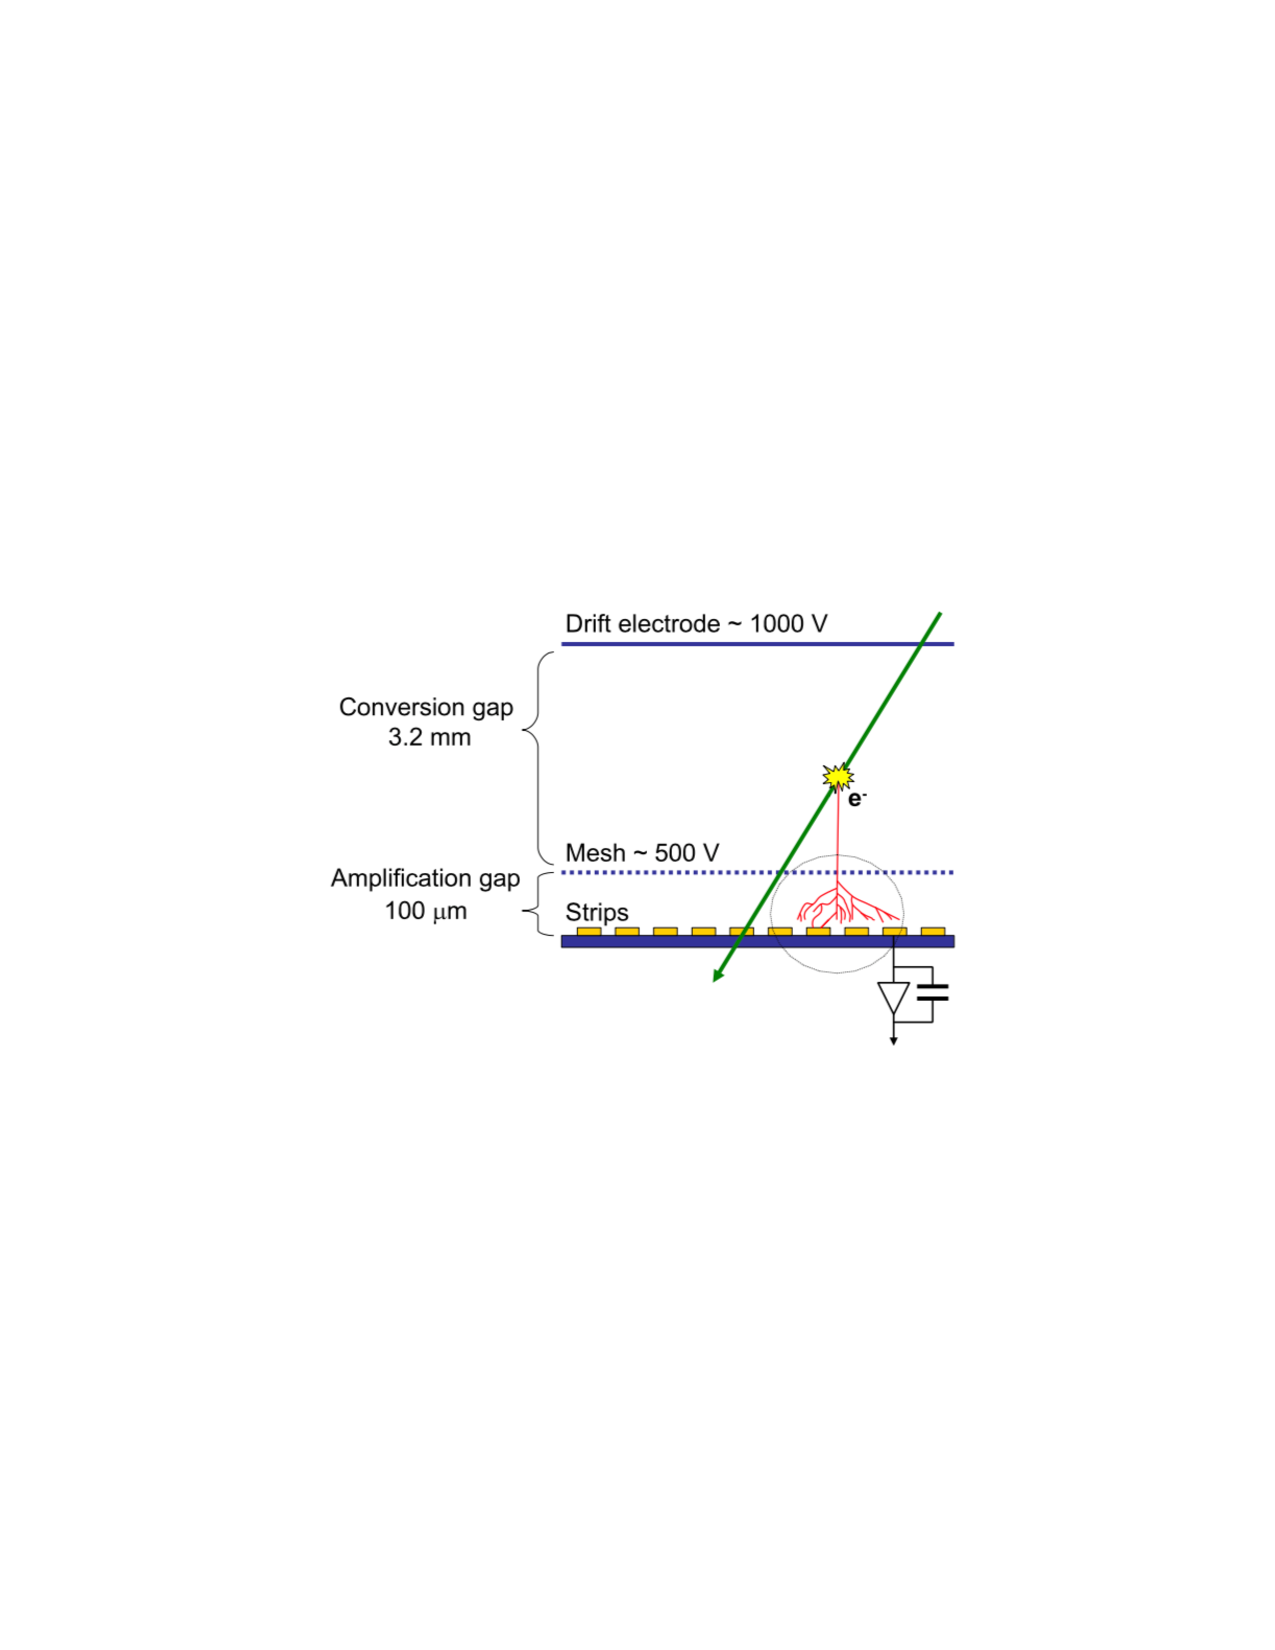
\includegraphics[width=0.7\textwidth, trim=4cm 10cm 4cm 10cm, clip]{MicroMega}
  \caption{Principle of operation for the micromesh gaseous structures
    (micromegas).  This image was taken from~\cite{compassSpec}.}
  \label{fig::MicroMega}
\end{figure}

There are eleven GEM detectors located throughout the COMPASS spectrometer.  The
first GEMs are located after the first spectrometer magnet and the last GEMs are
located near the end of the spectrometer.  These detectors are positioned close
to the beam axis.  Each of them is mounted on a large area tracker, covering the
dead zone region of the large area tracker.  All eleven detectors have an active
area of 31x31~cm$^2$ and a 5~cm diameter dead zone.  In times of lower beam
intensity, such as alignment runs, the dead zones can be turned on as an active
area.  \par

The GEM detectors are split into four regions where each region is separated by
a polymide foil (50~$\mu$m thick).  The polymide foil has approximately
10$^4$~cm$^{-1}$ drifting holes of 70~$\mu$m diameter, which are clad with
copper on both sides.  There is an electric potential of a few hundred volts
between each pair of foil layers.  The electron amplification occurs around the
holes of each of the three foil dividers.  This means GEM detectors speed up the
amplification process by splitting the amplification avalanche into three
locations.  The process is sped up because the drifting electrons are
accelerated multiple times, thereby speeding up their drifting velocity which
therefore reduces the overall drift time from the ionization location to the
strip readout.  This allows the GEMs to operate at a higher rate then would
otherwise be possible.  The principle of operation is illustrated in
Fig.~\ref{fig::GEM}.  The nominal timing and spacial resolution of the GEM
detectors is 10~ns and 110~$\mu$m respectively.  Two pixelized GEM detectors
were also in operation but were not as crucial for the 2015 Drell-Yan
measurement.

\begin{figure}[h!t]
  \centering
  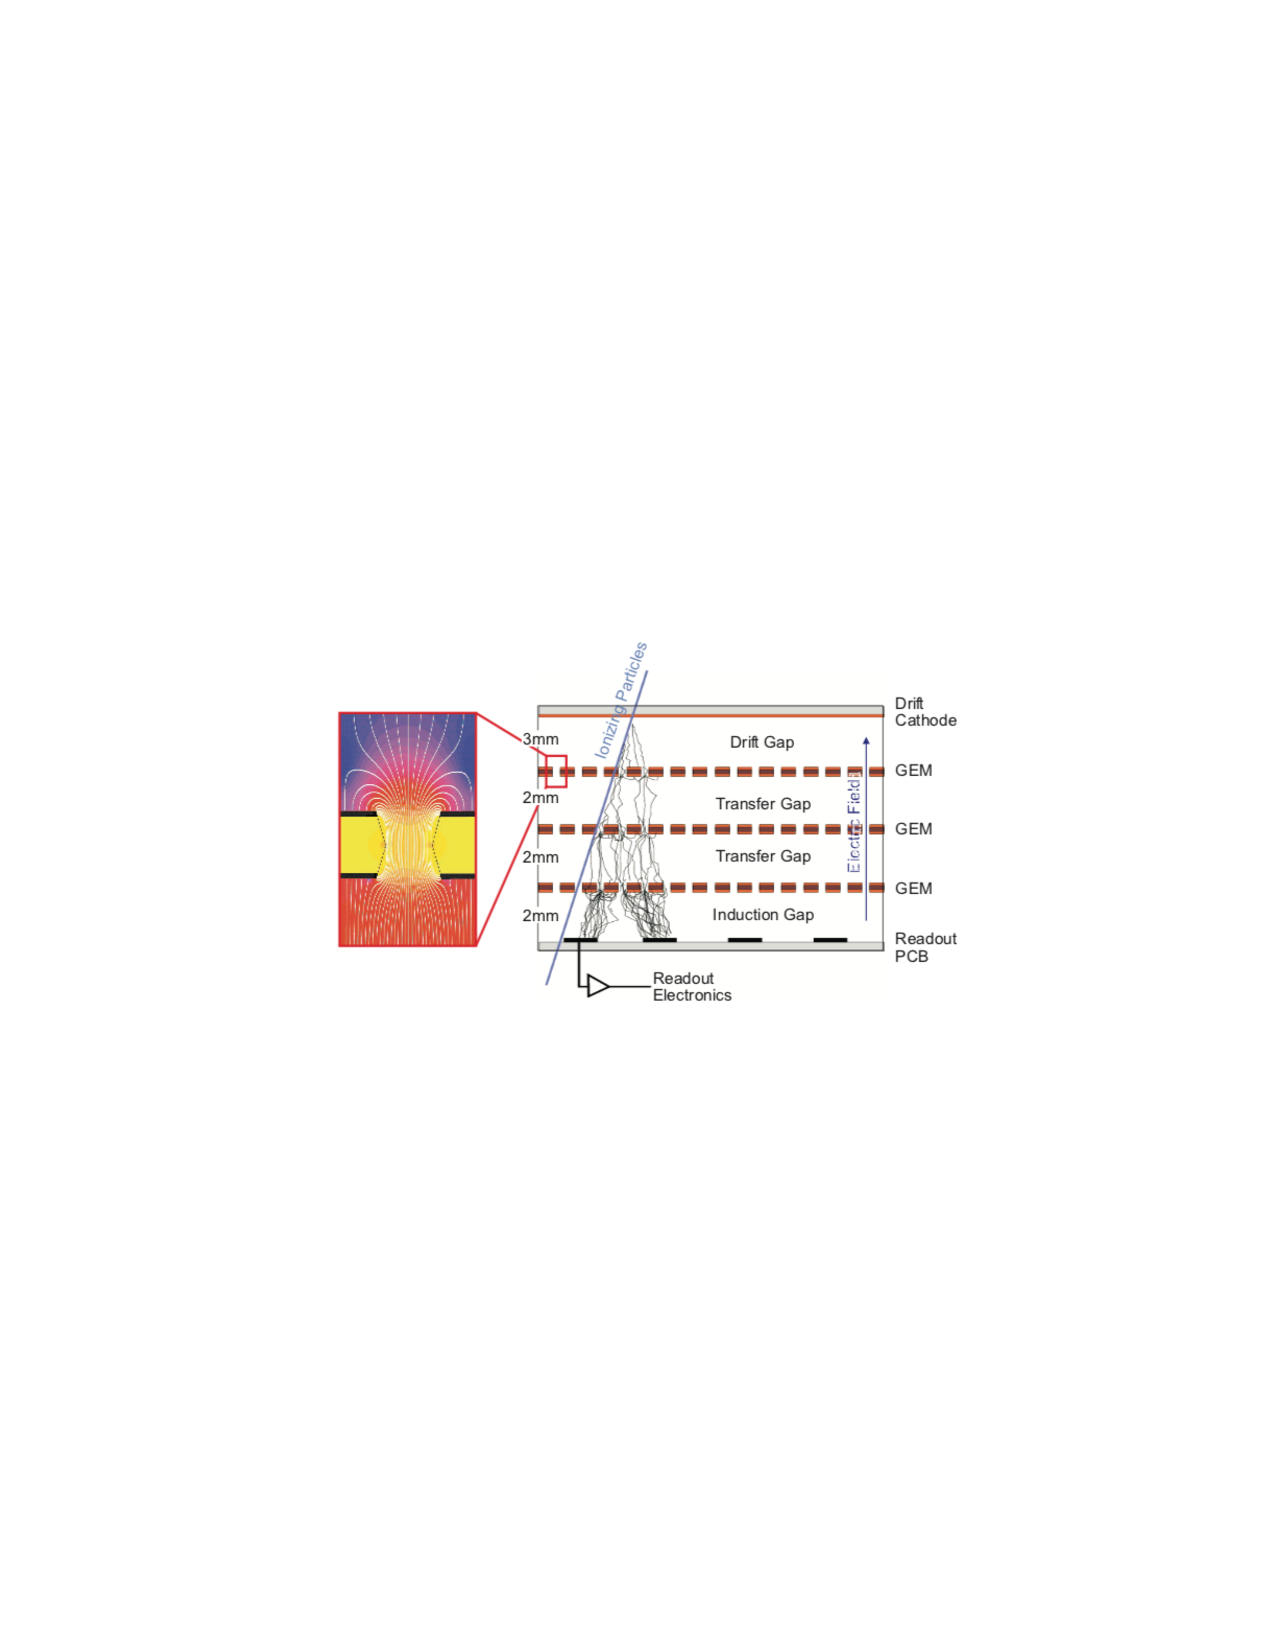
\includegraphics[width=0.7\textwidth,trim=4cm 10cm 4cm 10cm, clip]{GEM}
  \caption{The operation principle of the gas electron multiplier (GEM)
    detectors.  This image was taken from~\cite{compassSpec}.}
  \label{fig::GEM}
\end{figure}

\subsection{Large Area Trackers}
The large area trackers measure the largest polar scattering angles at COMPASS.
Their dead zones mostly coincide with a small area tracker, described in the
previous section~\ref{sec::SAT}, which therefore means these detectors do not
have to process the higher fluxes very close to the beam line.  The most
important feature of these detectors is that they have a large planar area. As a
consequence however, their position and timing resolutions are not as good as
the small and very small angle trackers.  The types of large area trackers used
at COMPASS are all gaseous detectors and include drift chambers (DCs), straw
tube detectors (straws) and multi-wire proportional chambers (MWPCs). \par

The first four drift chambers downstream of the target are named DC00, DC01,
DC04 and DC05.  The first two, DC00 and DC01, have smaller active areas of
180x127~cm$^2$ and a circular dead zone of 30~cm diameter.  These two drift
chambers are positioned upstream of the SM1 magnet.  The rates upstream of SM1
are higher.  This is due to the fact that low energy particles are produced in
the target, but are bent out of the acceptance of spectrometer by SM1.
Therefore the detectors downstream of SM1 do not track these low energy
particles and therefore DC00 and DC01 need to be able to process a higher
particle flux.  The next two drift chambers, DC04 and DC05, are downstream of
SM1 and both have larger active areas of 240x204~cm$^2$ and as well have dead
zones of 30~cm diameter.  The active areas of all four of these DCs was roughly
chosen to coincide with the acceptance of the SM1 yoke.  DC05 was first
installed for the 2015 Drell-Yan data taking and is further described in
chapter~\ref{ch::dc05}.  All four of these DCs measure four projection views
corresponding to eight detector layers.  A sketch of the principle of operation
is shown in Fig.~\ref{fig::DCoperation}.  The nominal spacial resolution for
these detectors is 250~$\mu$m. \par

\begin{figure}[h!t]
  \centering
  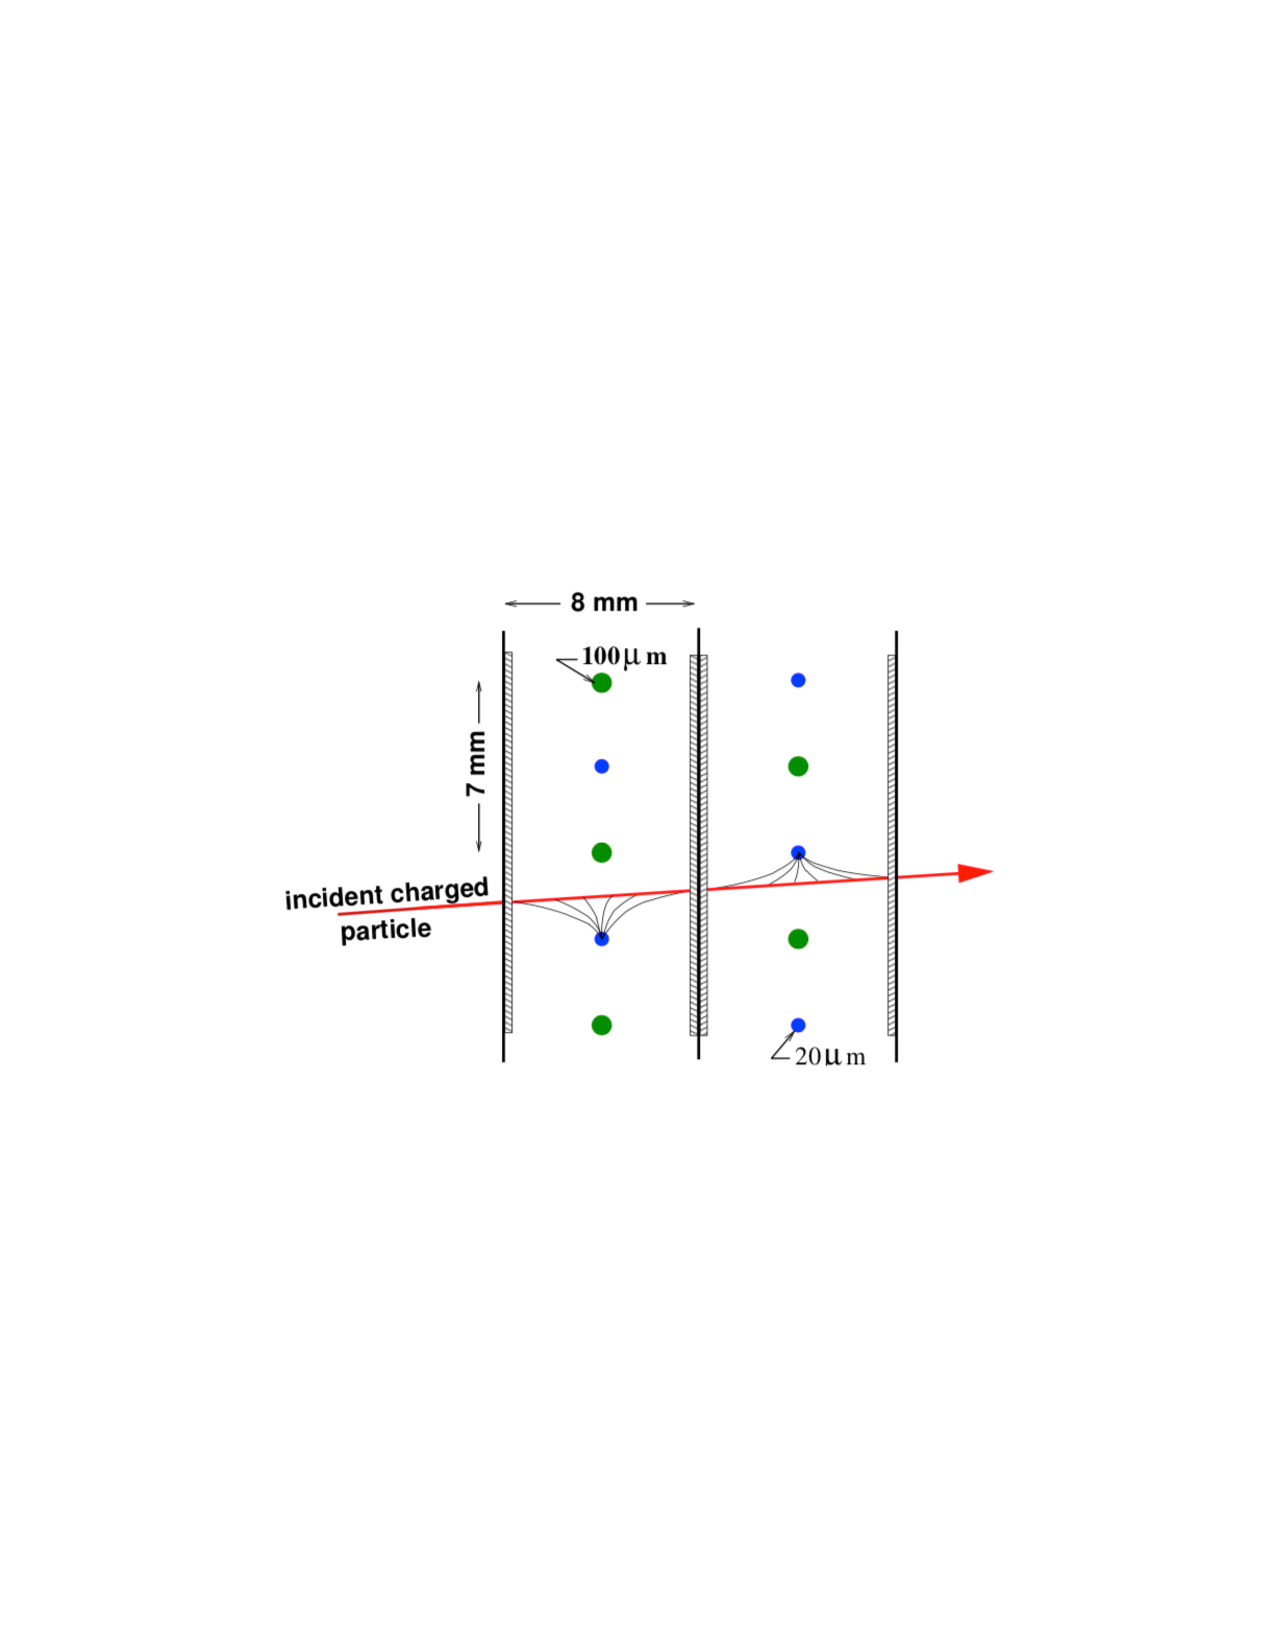
\includegraphics[width=0.6\textwidth,trim=4cm 8cm 4cm 10cm,
    clip=true]{DCoperation}
  \caption{Side view of a drift cell in a drift chamber with the ionized drift
    electron lines coming from the incident charged particle.  The larger
    circles (green) represent field wires and the smaller circles (blue)
    represent sense wires.  This image was taken from~\cite{compassSpec}.}
  \label{fig::DCoperation}
\end{figure}

Further downstream the spectrometer, downstream of the SM2 magnet, are the W45
drift chamber stations.  The W45 drift chambers are the largest drift chambers
at COMPASS.  There are six W45 detector stations, which each have an active area
of 520x260~cm$^2$ and a circular dead zone of 50~cm or 100~cm diameter.  Each
W45 station measures two projection views corresponding to four detector layers.
The drift cells in W45 are 40x10~mm$^2$ and the spacial resolution is nominally
1500~$\mu$m. \par

The two straw stations in operation during the 2015 data taking are named ST03
and ST05.  ST03 was in the large angle spectrometer downstream of DC05 and
consists of two stations measuring six projection views.  ST05 was in the small
angle spectrometer and measured three projection views.  The active areas of
each of the horizontal wire stations is 350x243~cm$^2$ and the active area of
each of the rotated wires is 323x272~cm$^2$.  The principle of operation for the
straw detectors is very similar to that of a drift chamber.  However, instead of
having the detector made up of connected drift cells the straw detectors are
made of separated circular tubes.  Each tube consist of a gold plated tungsten
anode wire in the center and the walls of the tube make up a cathode.  Due to
the fact that the cathode completely surrounds the anode wire there is no
electrical interference between neighboring anode wires as there is for drift
chambers.  For this reason the electric field in each tube is easier to control
and the ionized electron drift speed is more linear than other detectors.  Each
straw detector plane is divided into sections where the straw tubes in the outer
most section from the beam line have a diameter of 9.6~mm and the tubes close to
the beam line have a diameter of 6.1~mm.  In addition, in the central part of
the detector there is a physical hole, dead zone of 20x20~cm$^2$.  The nominal
position resolution for these detectors is 400~$\mu$m.  A frontal schematic is
shown in Fig.~\ref{fig::frontalStraw}.  For the reason that most of the detected
muons are reconstructed in the large angle spectrometer and the fact that many
of the high voltage modules were not operation for ST05 in 2015, ST05 was not
used for track reconstruction for 2015 Drell-Yan data. \par

\begin{figure}[h!t]
  \centering
  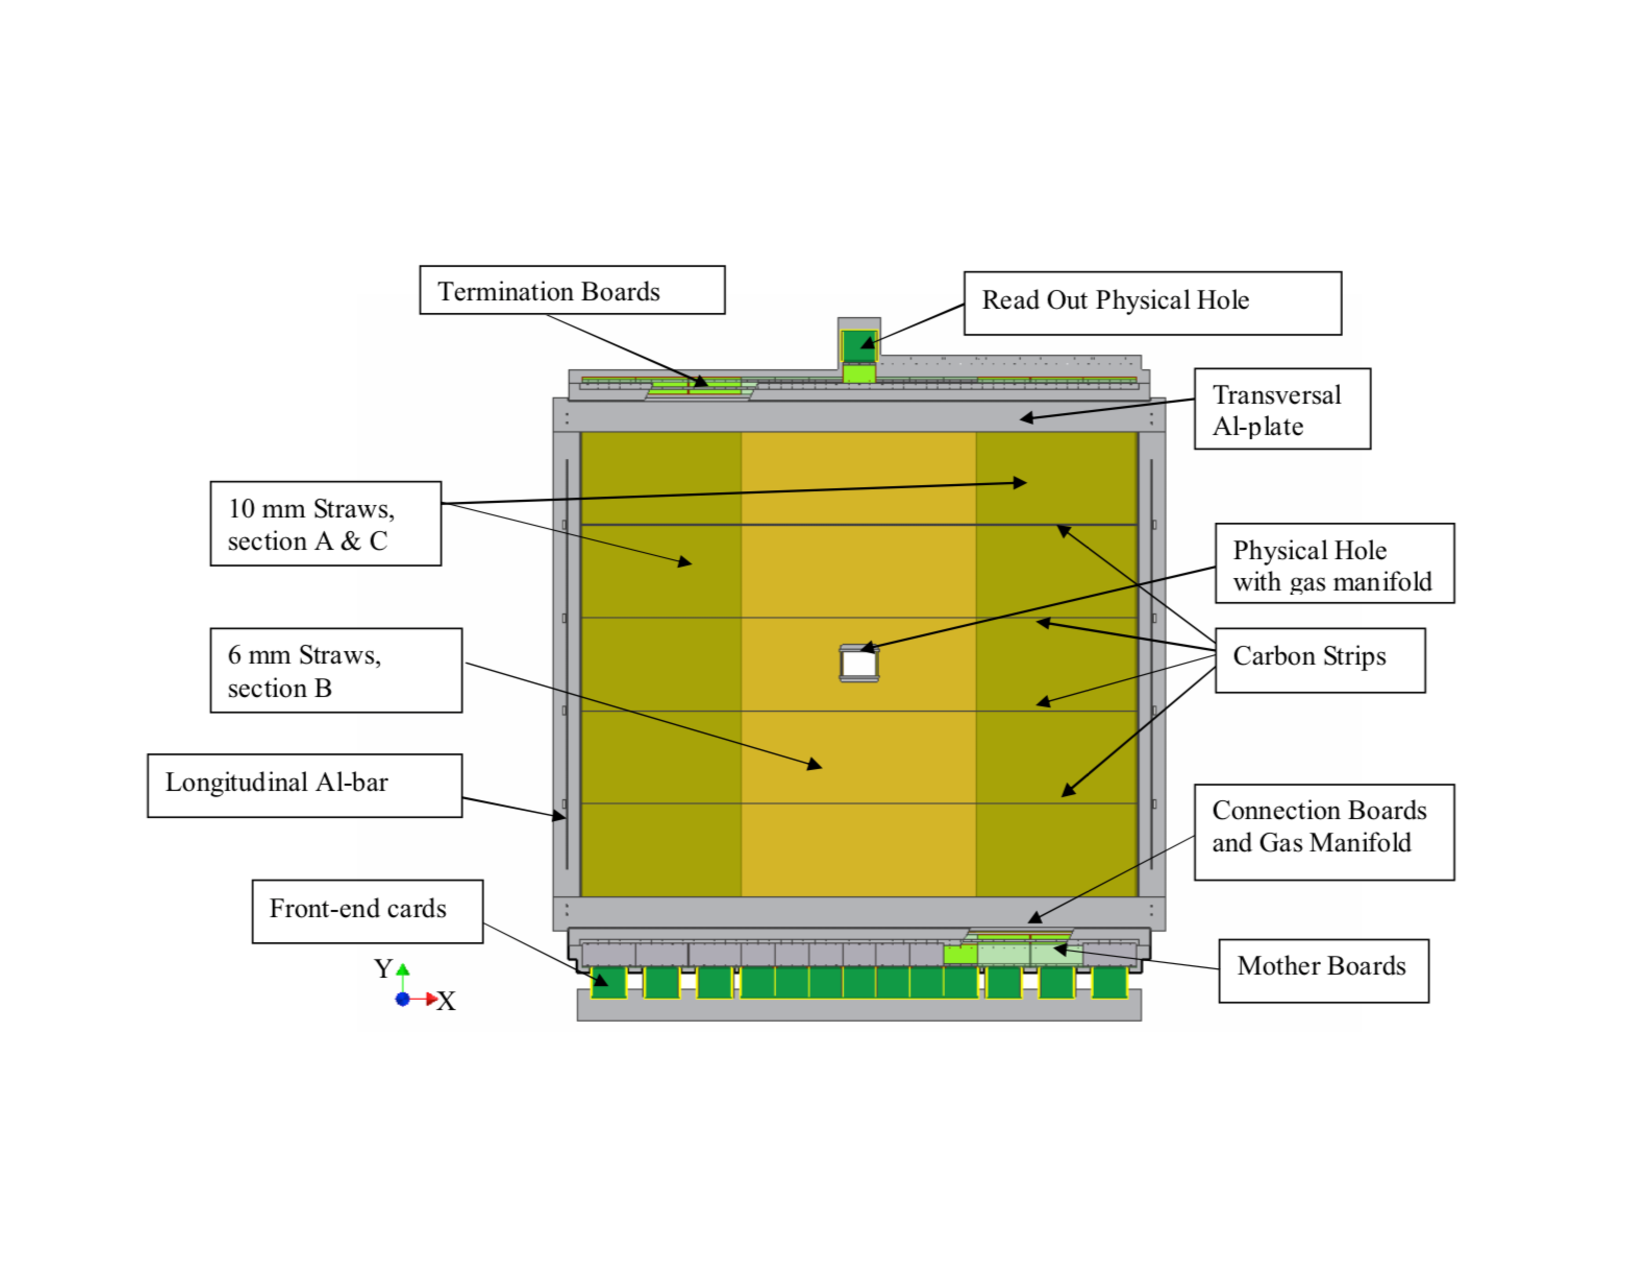
\includegraphics[width=0.8\textwidth,trim=2cm 4cm 3cm 4cm,clip]{frontalStraw}
  \caption{Front on view of a the active area of a straw detector at COMPASS.
    This image was taken from~\cite{compassSpec}.}
  \label{fig::frontalStraw}
\end{figure}

The next type of large angle track is the richwall.  This large area tracker
operates similarly to the straw tube detectors.  The detector consist of eight
layers of mini drift tubes (MDT) shown in Fig.~\ref{fig::richwallMDT}.  The
central part of each MDT includes a gold plated tungsten sense wire.  The
richwall is located upstream of the SM2 magnet and downstream of ST03.  The
richwall has an active area of 5.27x3.91~cm$^2$ and a central dead zone of
1.02x0.51~cm$^2$.  The nominal position resolution of this detector is
600~$\mu$m. \par

\begin{figure}[h!t]
  \centering
  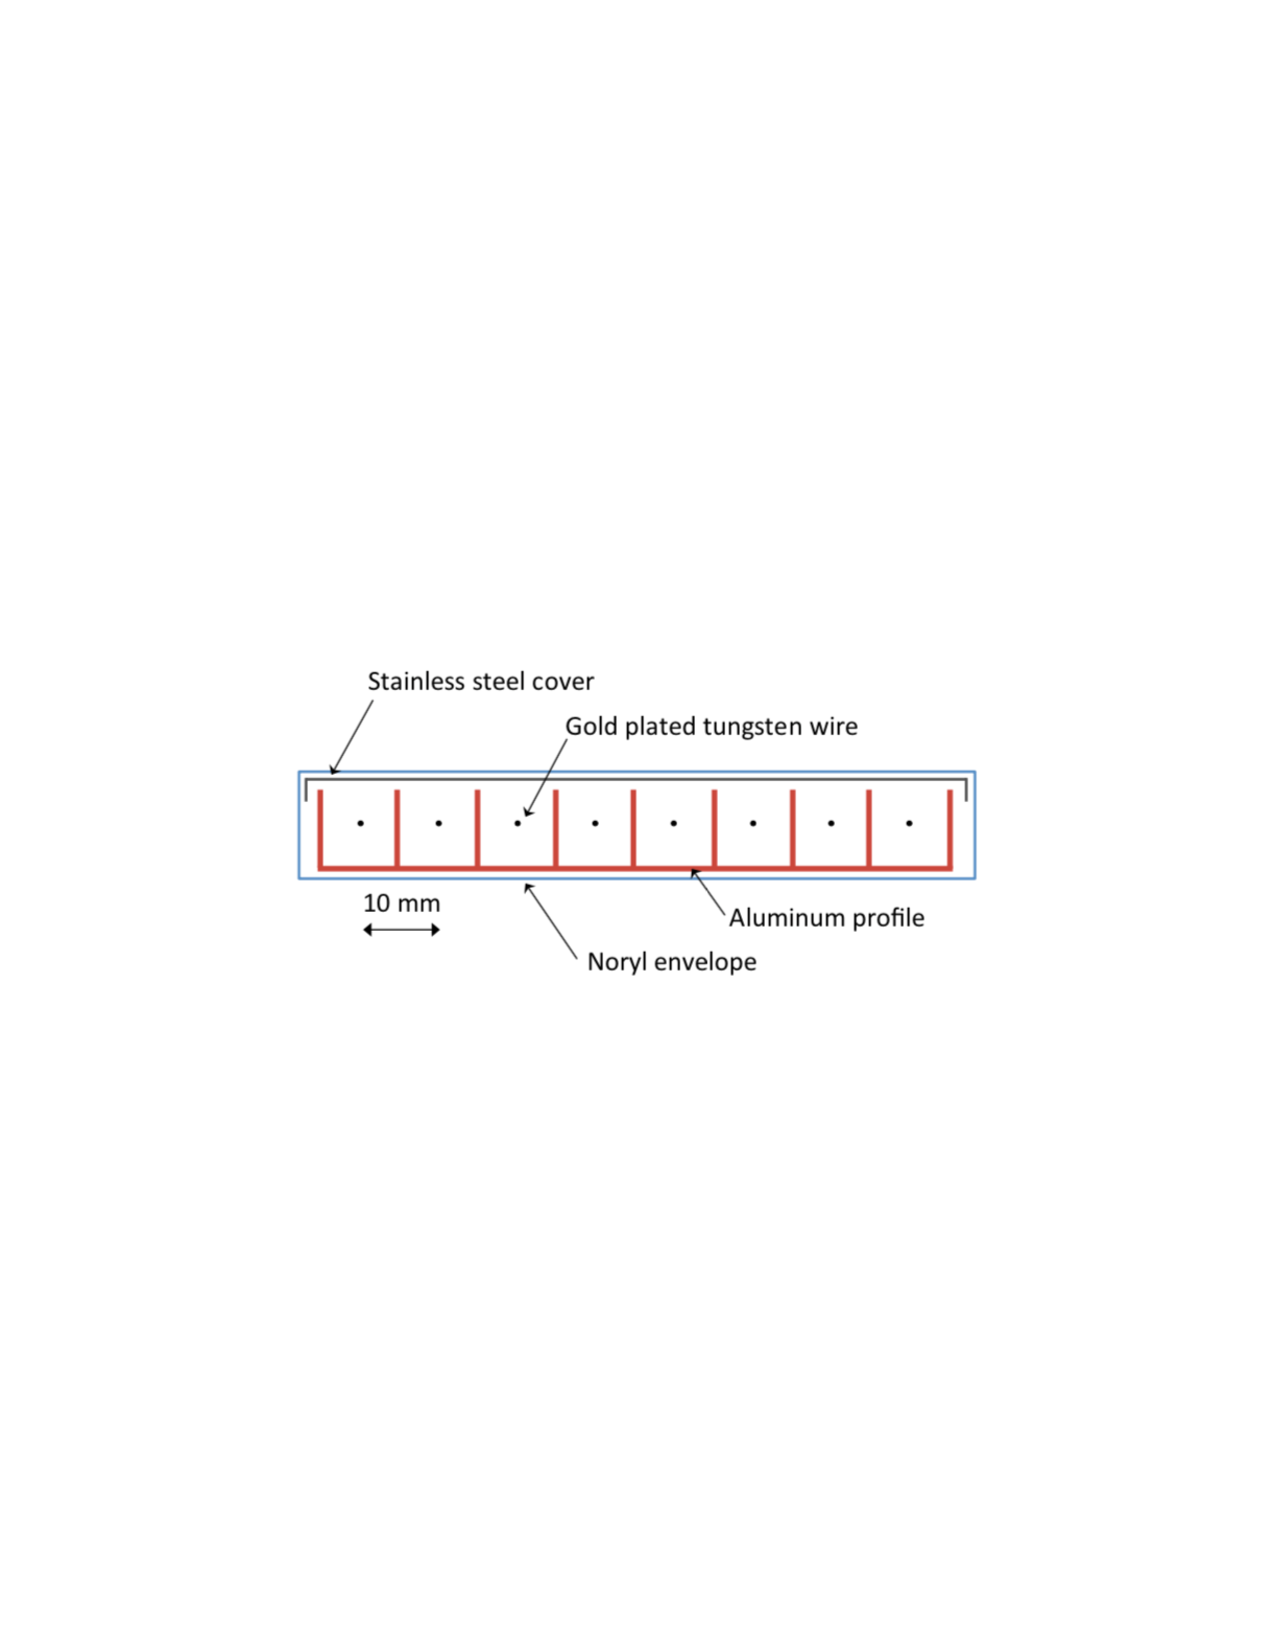
\includegraphics[width=0.45\textwidth, trim=5cm 12cm 5cm 10cm, clip]
                  {richwallMDT}
  \caption{The richwall mini drift tubes.  This image is taken
    from~\cite{ABBON201569}.}
  \label{fig::richwallMDT}
\end{figure}

The final type of large area tracking detector at COMPASS is the MWPC.  There
are 14 of these stations located throughout the experiment.  The MWPCs are
separated into three categories distinguished by the coordinates they measure.
The first type is called type A and consists of three projection views measuring
an x, u and v coordinate.  The second type is type A* and is the same as type A
but measures the y coordinate in addition to the other three coordinates.  Both
type A and A* have active areas of 178x120~cm$^2$.  The final type is type B
which has a smaller active area of 178x90~cm$^2$ and measures the same
projections as type A.  There are seven stations of type A, one station of type
A* and six stations of type B.  All three types have circular dead zones of
diameters 16~cm, 20~cm and 22~cm for types A, A* and B respectively. \par

The MWPCs operate on similar principles to the drift chambers but without a
calibration drift curve.  For this reason the MWPCs can be made to have one
common gas volume between each station.  Their position resolution is
determined as

\begin{equation}
\frac{\mathrm{sense \: wire \: separation}}{\sqrt{12}},
\end{equation}
\noindent
which is the variance of a uniform distribution.  The separation between sense
wires is approximately 2~mm which corresponds to a spacial resolution of these
detectors of around 600~$\mu$m.


\section{Particle Identification}
In the COMPASS spectrometer there are four types of detectors used to determine
particle identification (PID).  These four detectors are the ring image
Cherenkov (RICH) detector, electromagnet calorimeters (ECAL), hadron
calorimeters (HCAL) and muon walls (MW).  The RICH distinguishes between pions,
kaons and protons; ECAL1 and ECAL2 measure the energy from photons and
electrons; HCAL1 and HCAL2 measure the energy from hadrons; and MW1 and MW2
distinguish muons from all other particles.  The RICH, ECAL1, HCAL1 and MW1 are
in the large angle spectrometer in that respective order along the beam line.
The small angle spectrometer includes ECAL2, HCAL2 and MW2 again in that
respective order along the beam line. \par

The RICH detector operates similarly to the CEDARS, section~\ref{sec::addBeam}.
In the RICH, Cherenkov radiation is emitted from particles traveling through it
at an angle dependent on the particle's velocity.  The RICH is filled with a
dielectric gas, C$_4$F$_{10}$, which as an index of refraction greater than air.
The momentum of a particle going through the RICH is determined from bending
radius around SM1.  Therefore once the RICH determines the entering particles
velocity, the mass of particles can be distinguished.  A sketch of the RICH and
its operating principle is shown in Fig.~\ref{fig::rich}.  To distinguish
between particles, the minimum momenta are: 2.5~{\gvc} for pions, 9~{\gvc}
for kaons and 17~{\gvc} for protons.  The maximum momentum the RICH can
distinguish between any of these particles is 50~{\gvc}. This detector is
located in the large angle spectrometer before any calorimeters.\par

\begin{figure}[h!t]
  \centering
  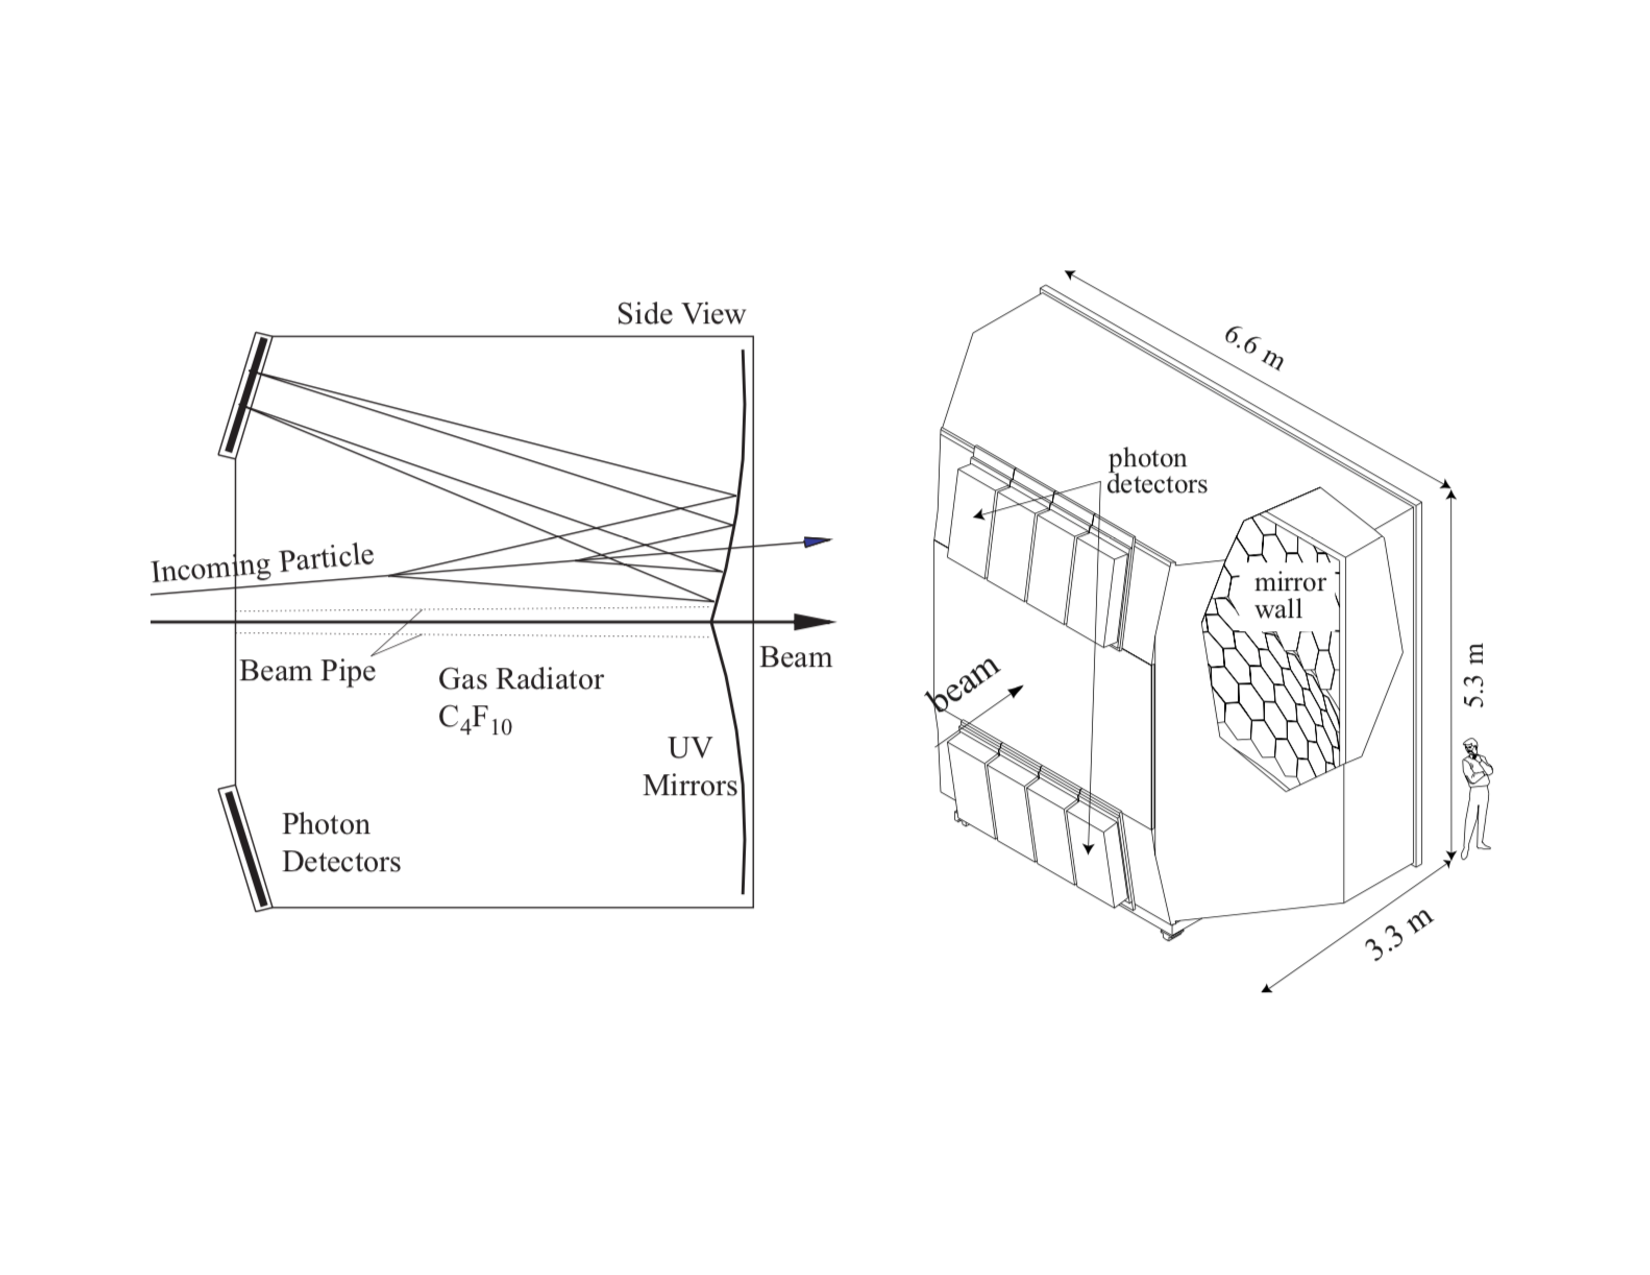
\includegraphics[width=0.6\textwidth, trim=1cm 5cm 1cm 4cm, clip]{rich}
  \caption{Side view demonstrating the principle of operation of the RICH
    detector.  This image was taken from~\cite{compassSpec}.}
  \label{fig::rich}
\end{figure}

The ECALs and HCALs both measure the energy of entering particles.  Both types
of calorimeters do this by stopping a specific entering particle, where the
amount of energy deposited in each respective calorimeter is proportional to the
incoming particle's energy.  ECALs are able to stop and measure electron and
photon energies and HCALs stop and measure hadron energies.  The energy
knowledge along with the momentum determined from the tracking detectors enables
the particle to be identified. \par

The ECALs are made of lead glass towers with photon multipliers attached to
these towers on one side.  An incoming photon or electron interacts with the
lead glass to produce a light signal, which is readout with these photon
multipliers.  Other particles also interact with the material in the ECALs
however hadrons and muons are able to exit through the detector unlike photons
and electrons.  A frontal view of ECAL1 is shown in Fig.~\ref{fig::ECAL1} and a
frontal view of ECAL2 is shown in figure Fig.~\ref{fig::ECAL2}. \par

\begin{figure}[h!t]
  \centering
  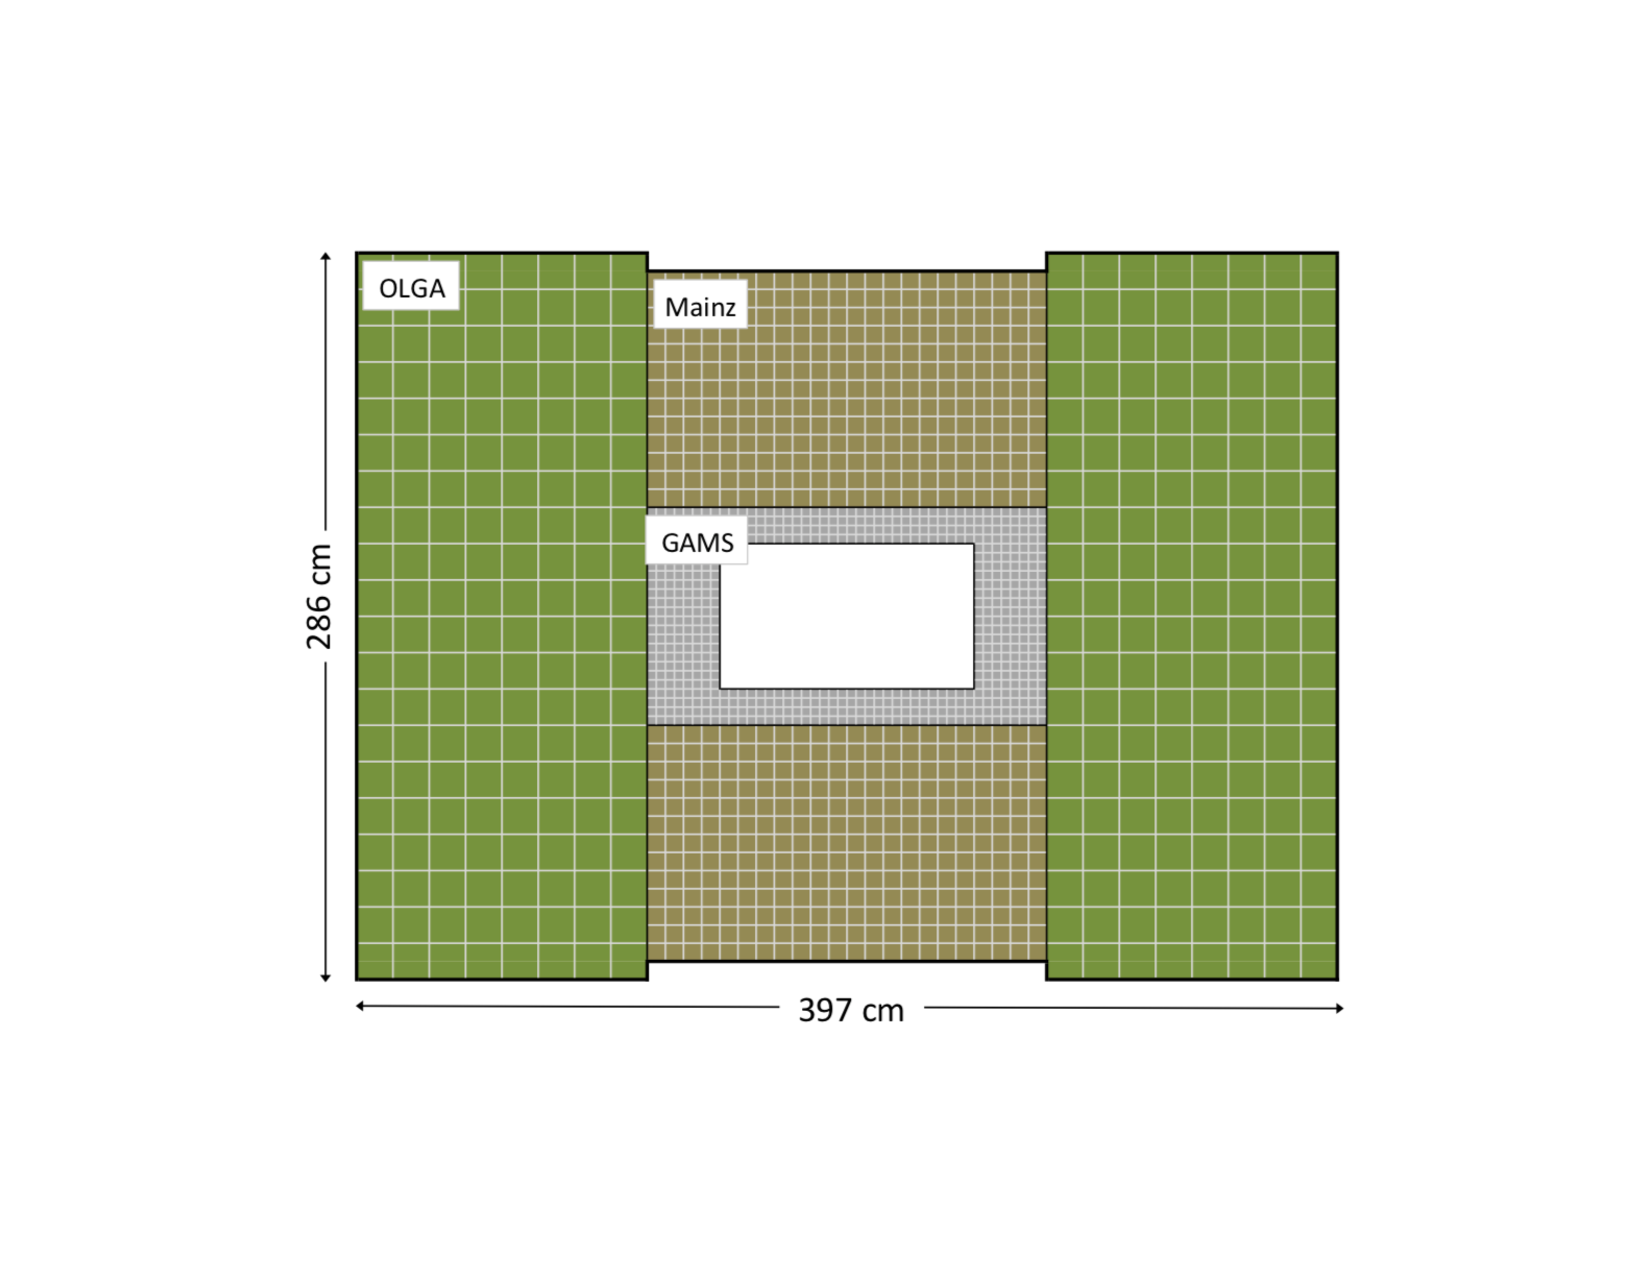
\includegraphics[width=0.6\textwidth, trim=4cm 4cm 4cm 4cm,clip]{ECAL1}
  \caption{Frontal view of the electromagnetic calorimeter 1.  This image is
    taken from~\cite{ABBON201569}.}
  \label{fig::ECAL1}
\end{figure}

\begin{figure}[h!t]
  \centering
  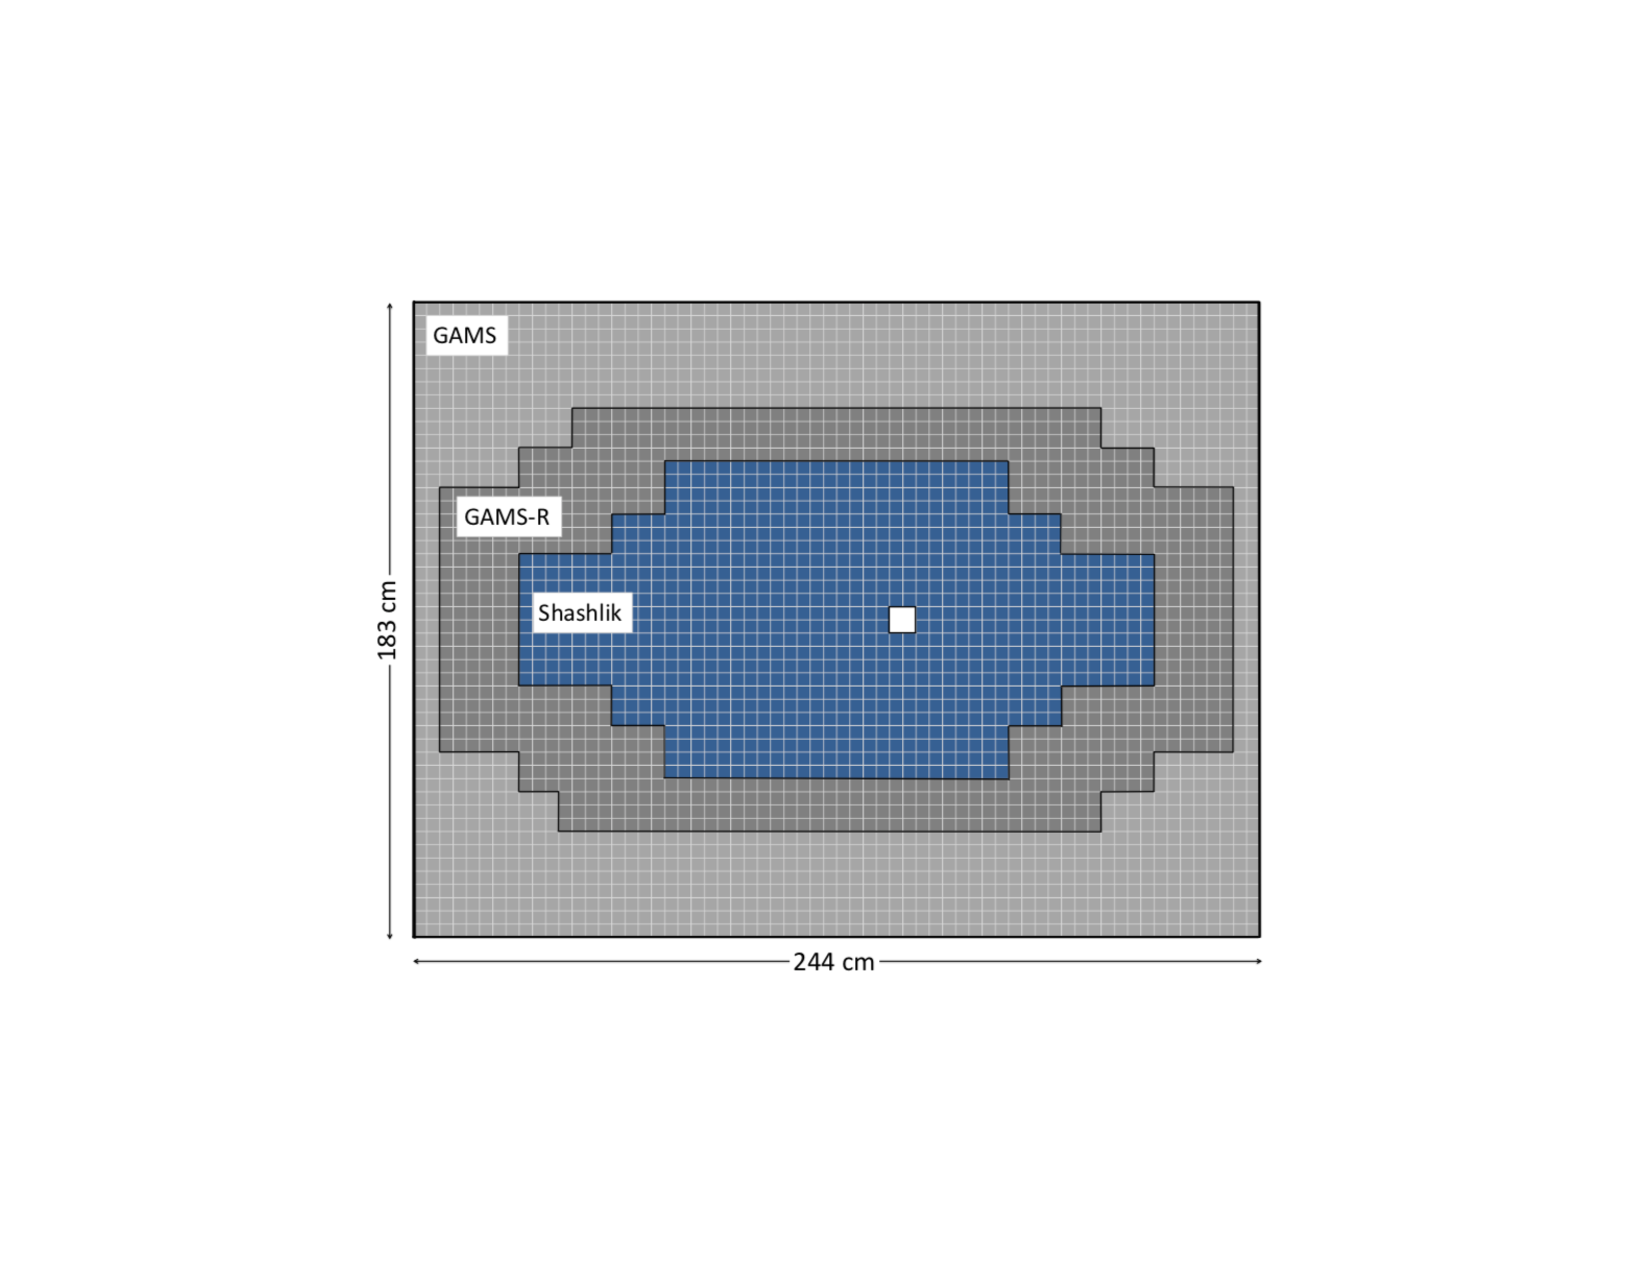
\includegraphics[width=0.6\textwidth, trim=4cm 4cm 4cm 4cm,clip]{ECAL2}
  \caption{Frontal view of the electromagnetic calorimeter 2.  This image is
    taken from~\cite{ABBON201569}.}
  \label{fig::ECAL2}
\end{figure}


The HCALs are sampling calorimeters, which are made of alternating layers of
iron and scintillating material.  An incoming hadron deposits all its energy in
the HCAL by making a particle shower in the iron.  This particle shower makes a
signal in the scintillating material, which is then read out by photo
multipliers.  The HCALs are placed after the ECALs in each stage of the
spectrometer because an electromagnetic shower happens within less material
budget than a hadronic shower.  The HCALs are effect at determining particle
energies from particle with energies between 10~GeV and 100~GeV. \par

The two MWs are located after an HCAL in their respective stages.  Due to their
higher mass and absence of color charge, muons are able to pass through the most
material budget of any of the particles detected at COMPASS.  For this reason
both MWs consist of an absorber and tracking detectors downstream of this
absorber.  Any particles that make it through the absorber are with a very high
probability muons. \par

MW1 consists of eight tracking planes before a 60~cm iron
absorber and the same number of tracking planes after this absorber.  The
tracking portions of MW1 are built similarly to the richwall, described in
section~\ref{sec::SAT}, in that they are also made of MDT modules.  The active
area of MW1 is 480x410~cm$^2$ and includes a dead zone of 140x80~cm$^2$.  Each
plane of this detector has a spacial resolution of 3~mm.  A sketch of MW1 is
shown in Fig.~\ref{fig::MW1}. \par

\begin{figure}[h!t]
  \centering
  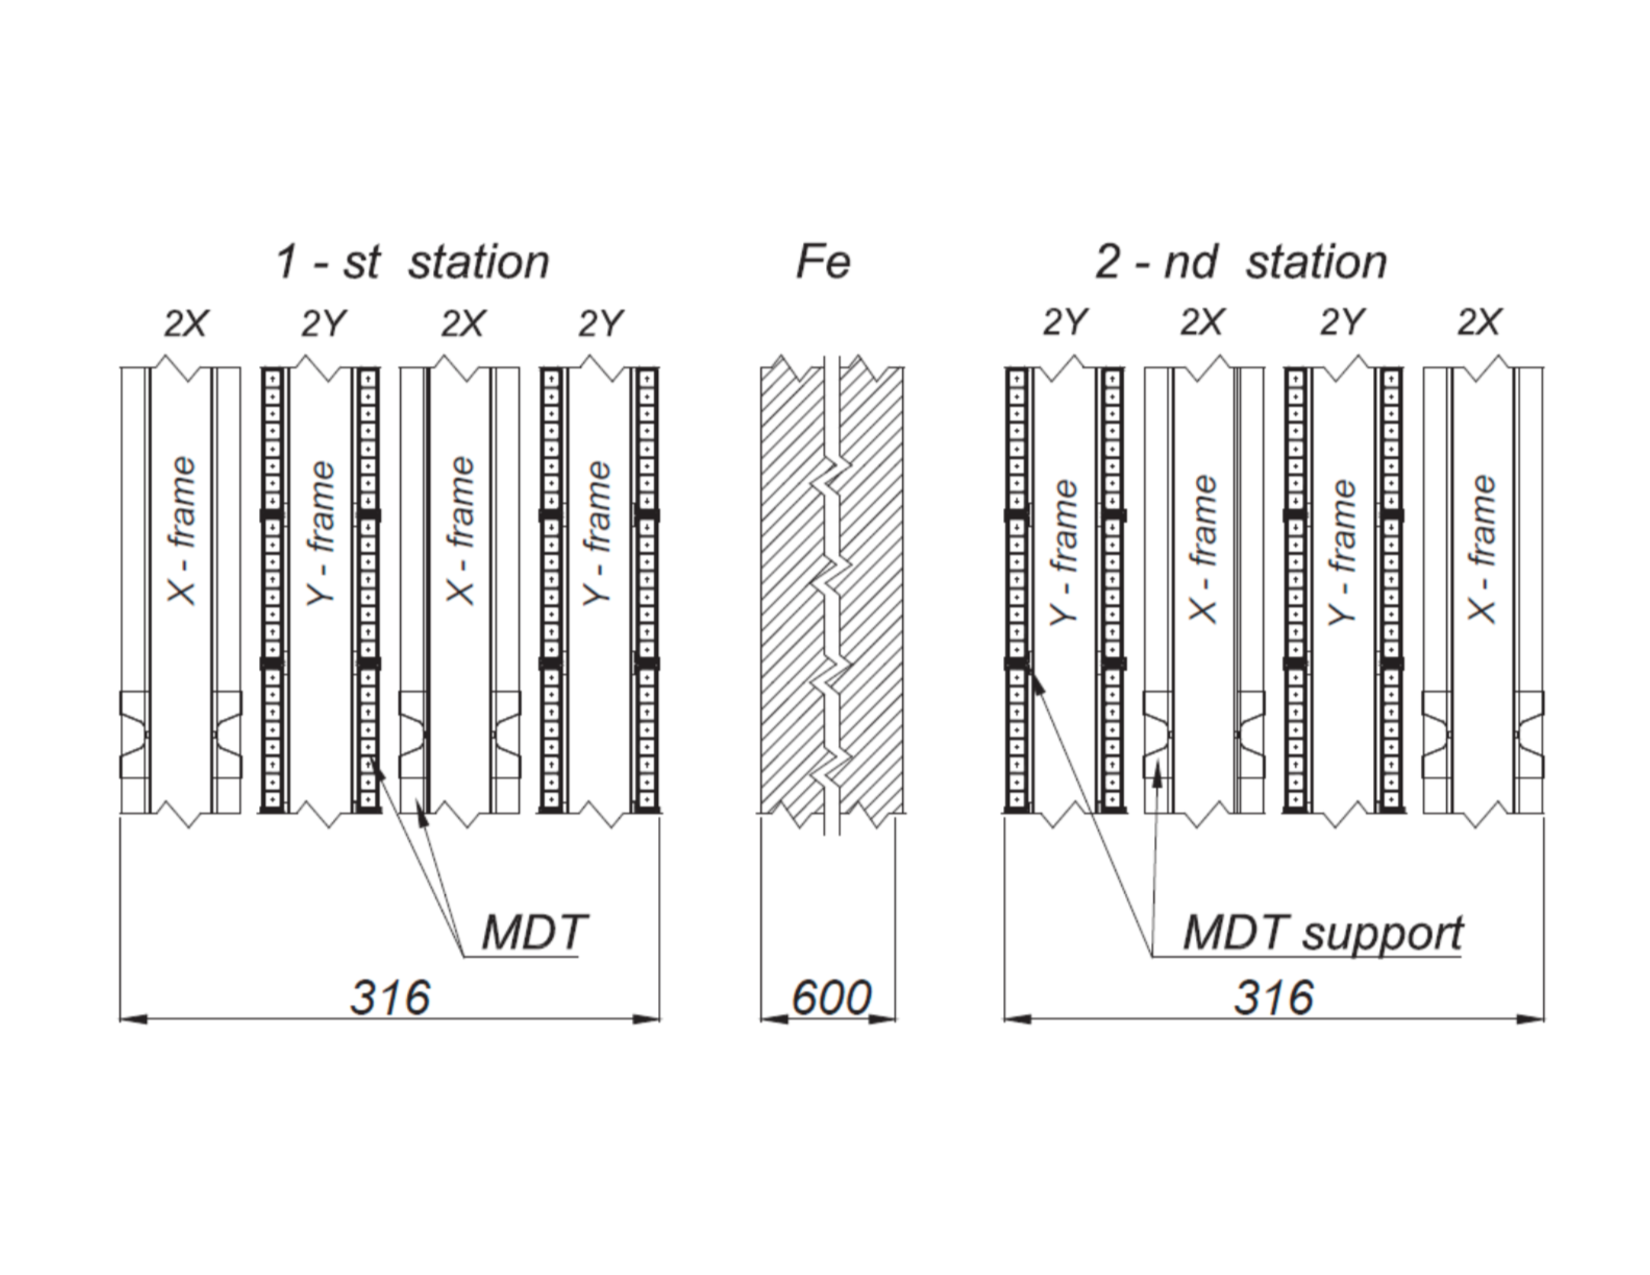
\includegraphics[width=0.7\textwidth, trim=1cm 3cm 1cm 3cm,clip]{MW1}
  \caption{A side view sketch of the muon wall 1 detector.  This image was taken
    from~\cite{compassSpec}.}
  \label{fig::MW1}
\end{figure}

The second muon wall, MW2, is located downstream of a 2.4~m thick concrete
absorber.  MW2 consists of 12 planes each with an active area of 450x450~cm$^2$
and a dead zone of 90x70~cm$^2$.  The detector operates similarly to the straw
detectors, section~\ref{sec::SAT}, in that the detector is made of drift tubes
with a wire in the center of these tubes.  The diameter of the drift tubes is
29~mm and the position resolution is about 1.4~mm. \par

There is one last absorber in the COMPASS spectrometer located before the H5
hodoscope at the end of the spectrometer hall.  This absorber is called muon
filter 3 (MW3) and ensures that the inner trigger is only triggered by a
muon. \par


\section{Trigger} \label{sec::trigger}
The trigger system at COMPASS defines what is an event.  Whenever the trigger
signal is given, all the detector information within a few nanosecond timing
window is recorded.  Due to the fact that there are very many background events
occurring as the beam impinges on the target, there is too much information
going to the front end modules (FEMs) of the detectors for the FEMs to process
and record all this information.  For this reason only a certain subset of all
the information is stored to disk.  The trigger system must therefore have good
timing resolution to make quick decisions on which data to record.  At COMPASS
the trigger systems consist of scintillating hodoscopes attached to PMTs.  The
timing resolution of these detectors is approximately 1~ns.  A top view
schematic of COMPASS showing where the relative positions of the hodoscopes for
each trigger is shown in Fig.~\ref{fig::TriggerElements}.  \par

\begin{figure}[h!t]
  \centering
  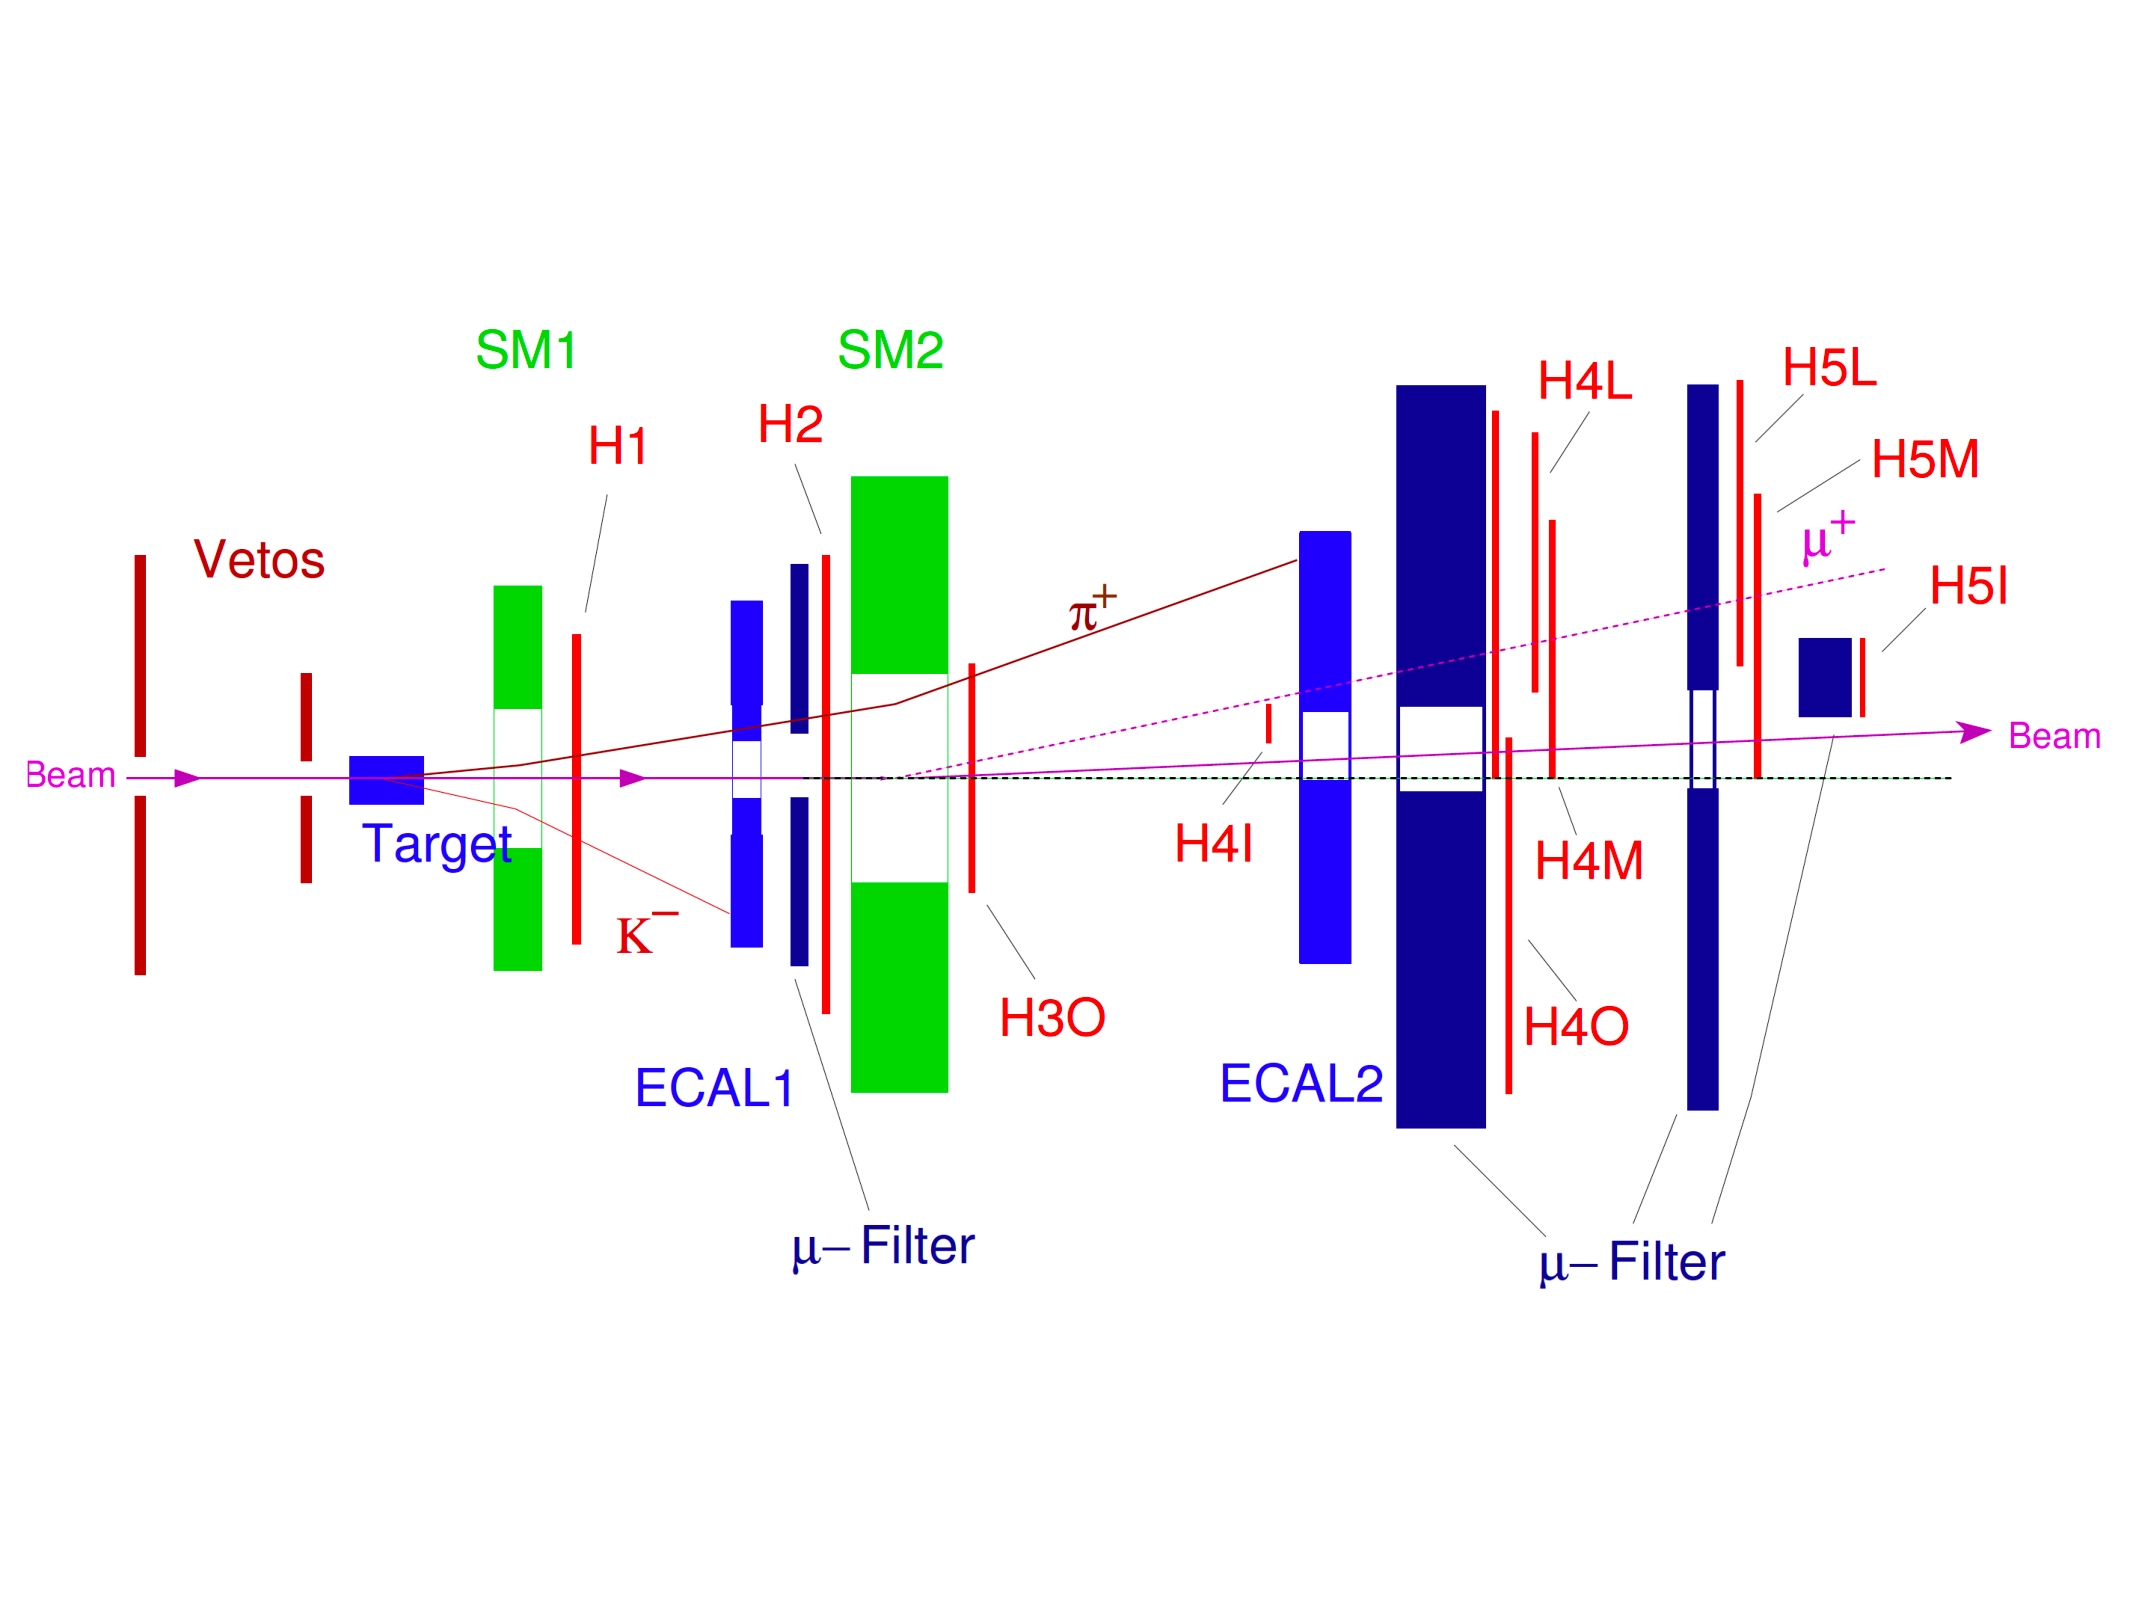
\includegraphics[width=0.9\textwidth]{TriggerElements}
  \caption{Top view of the spectrometer highlighting how different particles can
    signal a trigger.  This image was taken from~\cite{BERNET2005217}.}
  \label{fig::TriggerElements}
\end{figure}

At COMPASS there are five different triggers used to register physics events.
Each trigger type includes at least two hodoscopes at different z-positions in
the spectrometer.  The types of triggers are either target pointing, when the
hodoscope slabs are horizontal; or energy loss, when the hodoscope slabs are
vertical.  The target pointing trigger is setup and used with higher polar
scattering angles.  As the name suggest, this trigger signals when a particle is
scattered from the target.  The energy loss trigger is used to trigger on lower
Q$^2$ interactions and signals when a particle is bent a specified amount.
This concept is illustrated in Fig.~\ref{fig::TrigPrinc}.  \par

There are four triggers in SAS: the inner trigger (IT), the middle trigger (MT),
the ladder trigger (LT) and the outer trigger (OT).  The IT is an energy loss
trigger and includes the hodoscopes HI04X and HI05X.  The MT includes both
energy loss and target pointing slabs.  The hodoscopes in the MT are HM04X,
HM05X, HM04Y and HM05Y.  The MT hodoscopes whose names end with an X have
vertical slabs and those ending with a Y have horizontal slabs.  The LT is an
energy loss trigger which consists of HL04X and HL05X.  The final trigger in
SAS, the OT, is a target pointing trigger and consists of hodoscopes HO03Y and
HO04Y.  The remaining trigger system is in LAS and is a target pointing trigger
consisting of hodoscopes HG01Y and HG02Y.  The kinematic coverage for the 2015
triggers is shown in Fig.~\ref{fig::TrigCov6}. \par

\begin{figure}[h!t]
  \centering
  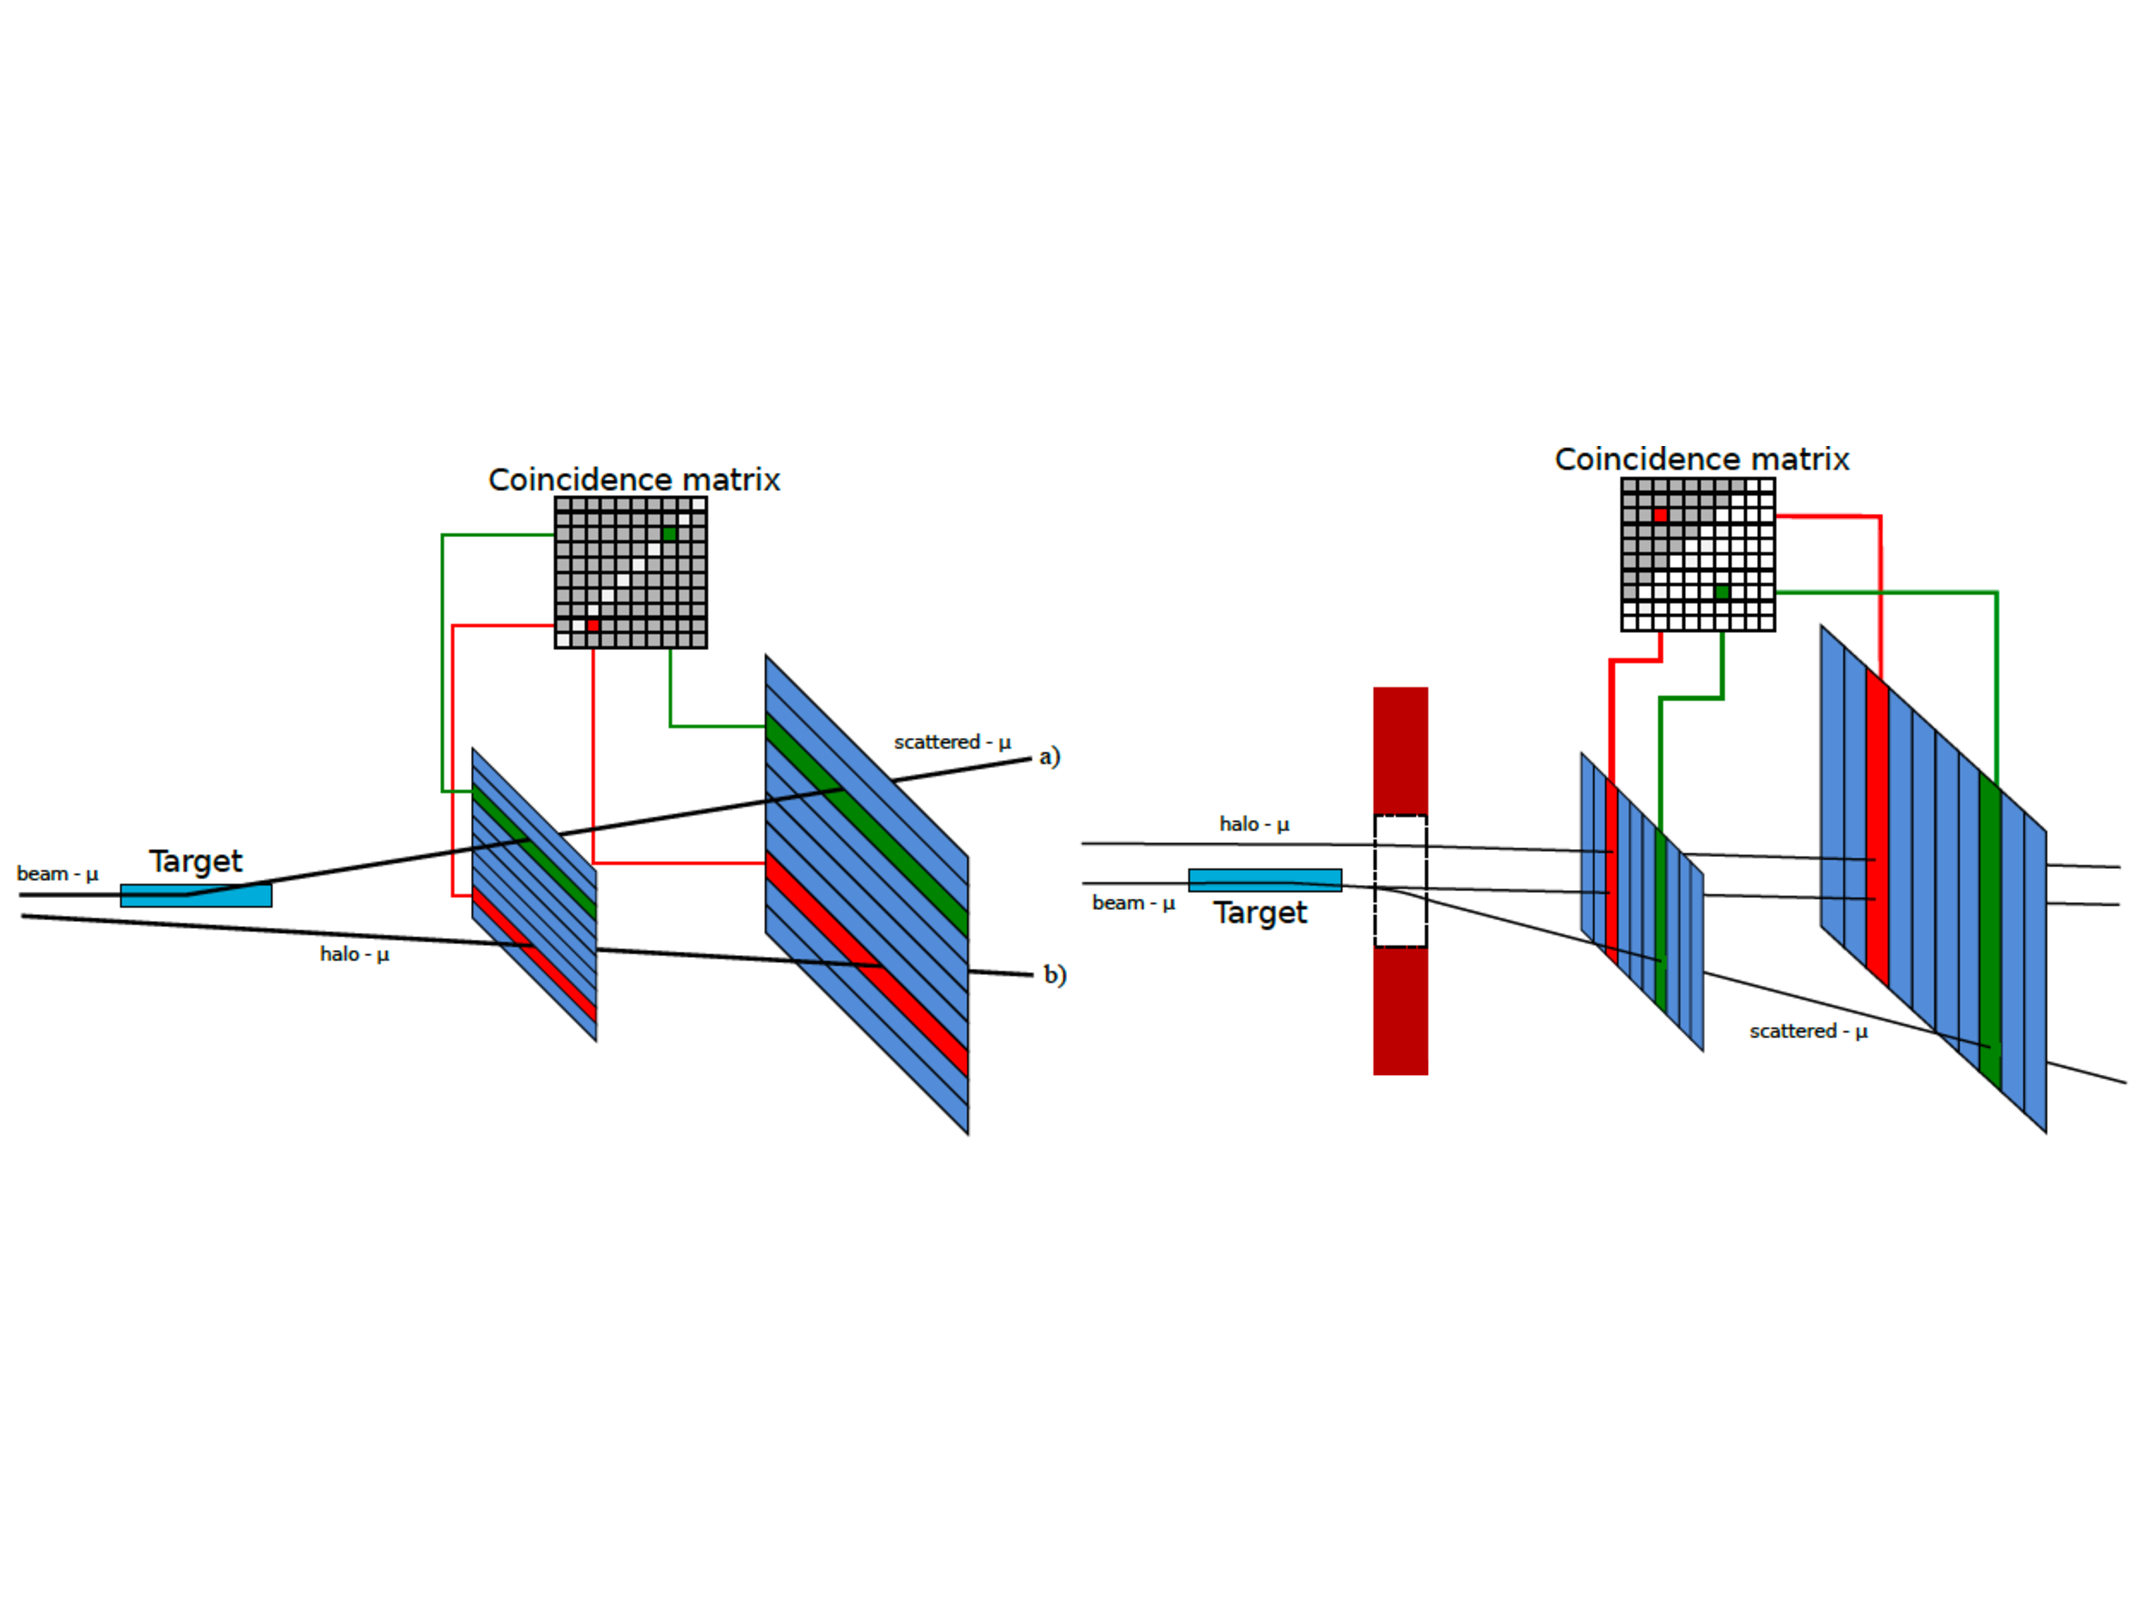
\includegraphics[width=0.9\textwidth]{TrigPrinc}
  \caption{The two types of triggers (left is target pointing and right is
    energy loss) at COMPASS and an illustration of the coincidence matrix used
    to select events of interest.  This image was taken from~\cite{trigDefs}.}
  \label{fig::TrigPrinc}
\end{figure}

\begin{figure}[h!t]
  \centering
  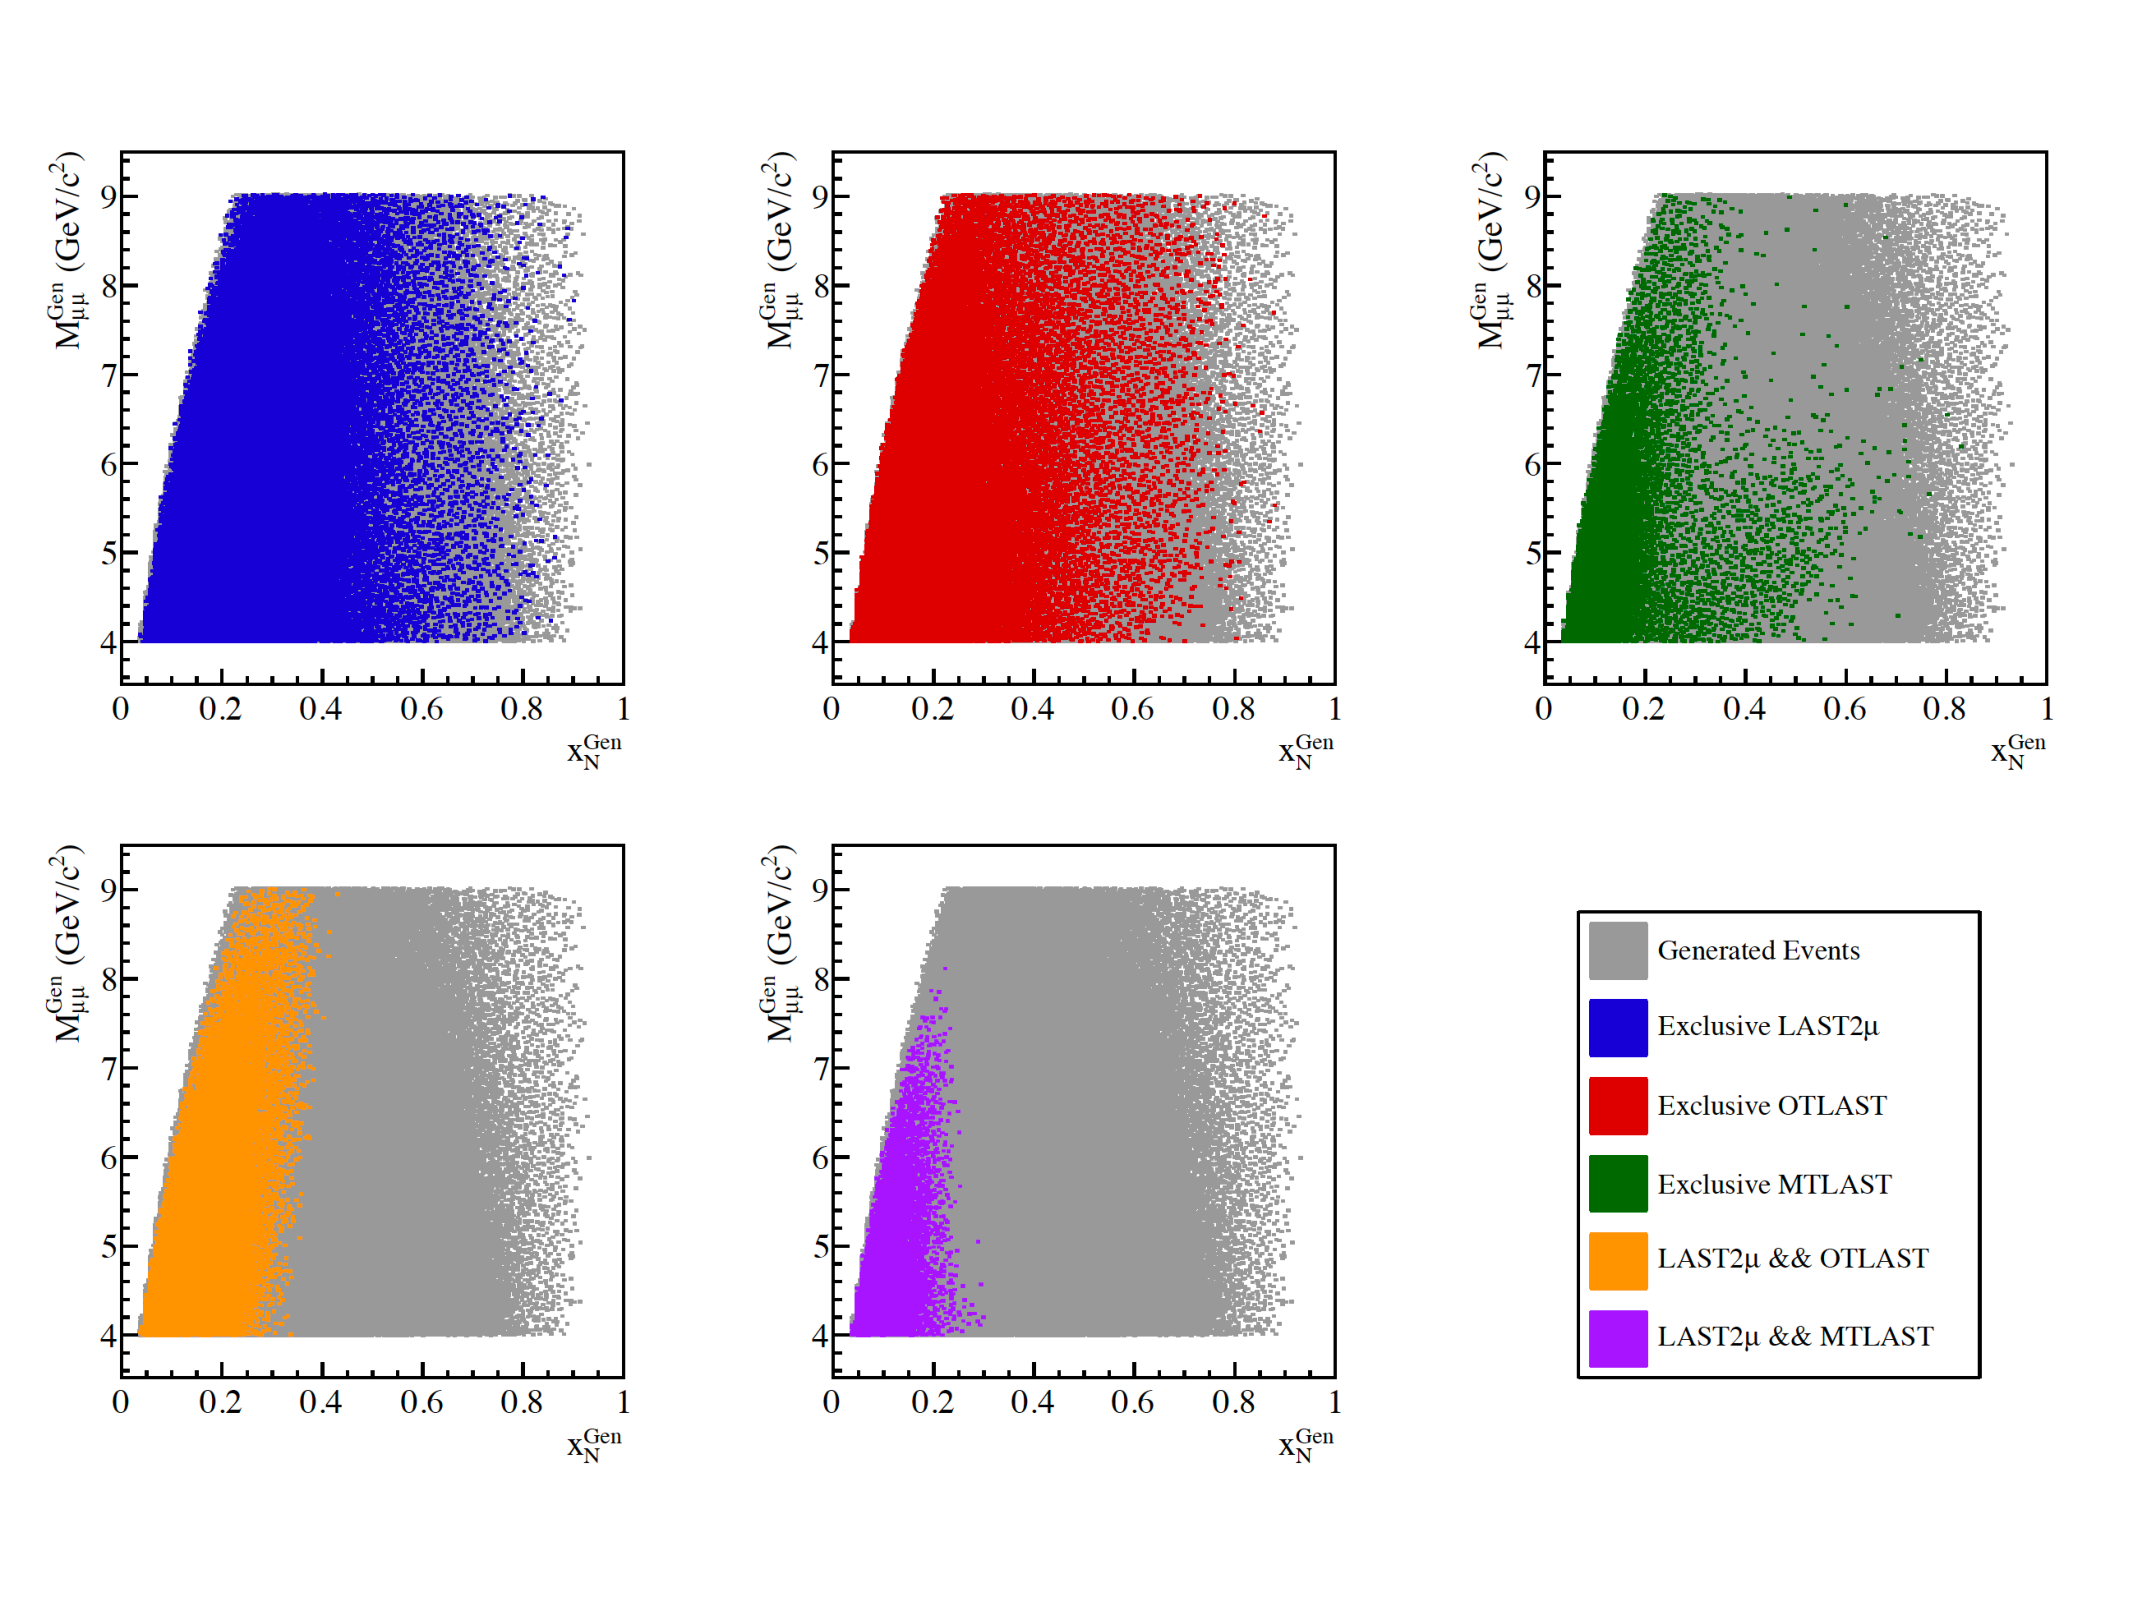
\includegraphics[width=0.9\textwidth]{TrigCov6}
  \caption{The kinematic coverage for the 2015 triggers determined from
    Monte-Carlo studies.  This image was taken from~\cite{longothesis}.}
  \label{fig::TrigCov6}
\end{figure}

In addition to signaling when interesting events occur, it is also import to
signal when background events are occurring.  For this reason there is also a
veto system upstream of the target as shown in Fig.~\ref{fig::TriggerElements}.
This veto trigger consists of hodoscopes attached to PMTs as well.  It is
centered on the beam axis but has a hole centered on the nominal beam line.  The
veto trigger is used to reject halo muons that surround the beam.  Halo muons
result from the beam decaying, as in Eq.~\ref{eqn::pionDecay} and
Eq.~\ref{eqn::kaonDecay}, where this decay occurs upstream of the target but
downstream of the ABS absorbers.  The muon halo surrounds the hadron beam due to
the muon's lower momentum, and it is for this reason that the veto hodoscopes,
outside of the beam line, are able to reject events that would occur due to the
halo.

There is one trigger in the spectrometer hall that is not a hodoscopes.  This is
the calorimeter trigger (CT).  The CT can be used as a trigger when a particle
deposits more than a certain energy threshold in the specified calorimeter.  In
2015 this trigger was only used as an independent study of the other triggers at
COMPASS. Particularly the CT was used to measure the trigger hodoscopes
efficiencies. \par

The last trigger used at COMPASS is a random trigger.  This trigger is setup
outside of the spectrometer area and registers a signal when a radioactive
source disintegrates.  In this way the random trigger is truly random.  In 2015
this trigger was used in studies of the beam flux.

In 2015, the goal was to measure two muons in the spectrometer.  For this
reason, two triggers must each signal a particle in coincidence for an event to
be registered.  For physics analysis the coincidence triggers are either two
muons in LAS (LASxLAS), one muon in LAS and one in the OT (LASxOT), or one muon
in LAS and one muon in the MT (LASxMT).  The LASxLAS trigger system covers the
high Q$^2$ and high x$_{\mathrm{beam}}$ phase space whereas the triggers
including a SAS hodoscope cover lower Q$^2$ values.  In addition to the dimuon
triggers there were three single muon triggers corresponding to a particle in
detected in LAS, MT or OT.  These three single muon triggers, however, where
pre-scaled down to record only one of every 500, 100 or 100 events respectively.
For further tests, 2015 included a random trigger and a beam trigger pre-scaled
down by 35000.


\section{Data Acquisition}
The data acquisition (DAQ) collects data from the over 250,000 detector channels
and transfers this data to storage on magnetic tape at CASTOR (CERN Advanced
STORage).  Despite the triggering system used to reduce the data rate, the data
still is recorded at event rates between 10~kHz to 100~kHz.  A typical COMPASS
event size is 45~kB.  The DAQ is designed to process these data rates and size
while minimizing the dead time associated with data collection and transfer. In
2015 the dead time was approximately 10\%.  The total data the DAQ recorded,
after the spectrometer finished commissioning, was approximately 820~terabytes
of raw data. \par

Data collection begins with the digitization of information from a detector
channel.  This digitization is performed by a time-to-digital converter (TDC) or
an analogue-to-digital converter (ADC). These TDCs and ADCs are either on the
detector FEMs or on custom COMPASS readout electronics named: GANDALF (Generic
Advanced Numerical Device for Analog and Logic Functions), GeSiCA (Gem and
Silicon Control and Acquisition) or CATCH (COMPASS Accumulate Transfer and
Control Hardware).  After digitization the data is transferred by optical fibers
to an FPGA multiplexer where the data is buffered by spill and arranged by
event.  From there an FPGA switch sends the data to multiplexer slaves.  The
slaves are online computers that oversee the final steps for raw data and
transfer this data to CASTOR.  

\section{Data Reconstruction}\label{sec::dataReconstruction}
The COMPASS Reconstruction and AnaLysis Program (CORAL) reconstructs the raw
data into physical quantities.  For example CORAL is able to convert the raw
data into particle tracks with momentum, charged and possibly an originating
vertex location~\cite{CORAL}.  The raw data from the DAQ is digitized timing
information from tracking detectors or digitized energy information for
calorimeters.  The process of reconstructing tracks takes the detector timing
information and determines a position in space for a particular tracking
detector based on a calibration.  CORAL then uses a Kalman Filter to determine
straight tracks in regions with no or low magnetic field~\cite{KalmanFilter}.
The tracks are then connected through the magnetic field using a fast lookup
table for known possible bending radii.  At this point a track is determined to
have a momentum, charge and an associated $\chi^2$ value.  From there the tracks
are extrapolated back to the target region and the intersection of at least two
tracks is determined as a vertex.  If in addition to the two intersecting
tracks, a beam particle can be extrapolated forward to the same vertex location
then the vertex is assigned to be a primary vertex.  Otherwise the vertex is
defined as a secondary vertex.

This reconstruction stage reduces the data volume by approximately a factor of
10.  In 2015 there were several data reconstructions performed.  Between each
reconstruction improvements were made to detector calibrations, detector
alignment, beam tracking and any other preprocessing improvements that could be
made.  The final two productions are the t3 production and the slot1 production.
The results shown in this thesis are from either t3 or slot1 productions.  The
slot1 production was the last production.  The difference between t3 and slot1
production is a new beam telescope reconstruction algorithm and an optimized
alignment which a new detector descriptions.  Specifically the hodoscopes for
triggers were changed to be described a detector split in half as oppose to a
detector split in fourths.  The changes between t3 and slot1 resulted in a 10\%
increase in events.

After reconstruction has been performed the data is stored in data structured
trees (DSTs).  The usual procedure of reconstruction which gives physical values
such as momentum and charge to tracks, results in data called miniDSTs.  There
is also the possibility to save more information, for example detector hit
location information, to make so-called fatDSTs.  These DSTs are in a format
which can be processed by PHAST (PHysics Analysis Software Tool).  PHAST is a
COMPASS program written to further analyze physics data.  With PHAST there is
the possibility to loop over all the miniDSTs and make certain kinematical cuts
and to produce so-called $\mu$DSTs based on these cuts.  In 2015 $\mu$DSTs were
made for all the analysis data where a cut was applied to the miniDSTs saving
only events with at least two muons.  Both CORAL and PHAST are fully
object-oriented C++ programs. \par

\subsection{Monte-Carlo Production}
Monte-Carlo data is simulated data which is performed in three steps.  First a
programs generates specific physics processes based on their theoretical
probabilities.  The generators of Monte-Carlo used for this thesis are PYTHIA
versions 6 and 8~\cite{pythia}.  Next a GEANT4 simulation of COMPASS determines
if a detector will register a hit from these generated physics processes.  This
saves the data in a raw data format which can be reconstructed by CORAL.
Finally the simulated data is reconstructed by CORAL and analyzed in PHAST the
same as if the data were real data. \par


\section{2015 Drell-Yan Data Taking} \label{sec::compass_2015_dy_setup}
The 2015 Drell-Yan data taking is one of the main programs for the COMPASS-II
experiment.  The data taking began in April of 2015 and ended in November of
that year.  The physics data used for analysis started in July and finished at
the end of data taking.  The data recorded before July was used for calibrations
and commissioning.  The total analysis data was split into nine data periods
labeled W07-W15 where each data period corresponded to approximately two weeks
of beam time. The spin orientation of each target cell was reversed after the
first sub-period of every period to reduce systematic effects arising from
different geometric acceptances and luminosities of the up and downstream target
cells. \par

\subsection{Hadron Absorber}
The previous sections in this chapter described the spectrometer setup generally
and mentioned the specifics for the 2015 setup.  The main unique hardware
addition in 2015 is the hadron absorber.  The hadron absorber was installed
because the beam intensity is high and results in many main strong interactions
in the target.  For this reason the first tracking detectors upstream of SM1
have occupancies that are too high for a satisfactory tracking performance.
Therefore the hadron absorber was installed to prevent all particles except
muons from entering the spectometer. \par

The hadron absorber was placed just downstream of the two target cells as can be
seen in Fig.~\ref{fig::Habs}.  The absorber corresponded to approximately 7.5
interactions lengths of material, where the material was mostly alumina
(Al$_2$O$_3$) and concrete.  Inside the absorber was an aluminum target followed
by a tungsten plug, each of radius 2.5 cm.  The tungsten was used as a beam
dump, while the aluminum was present to prevent back scattering from the
tungsten beam plug.  A side view showing the dimensions and materials used can
be seen in Fig.~\ref{fig::Abside}.  Both the aluminum target and tungsten plug
served the double purposes as absorbers and also as unpolarized nuclear targets.
In addition to the hadron absorber two 3~mm thick $^6\mathrm{Li}$ absorbers were
added just downstream of the primary absorber to absorb thermal neutrons
produced in the primary absorber.  This $^6\mathrm{Li}$ absorber was proposed to
improve the performance of the first tracking detector downstream of the target
even with the hadron absorber installed. \par

\begin{figure}[h!t]
  \centering
  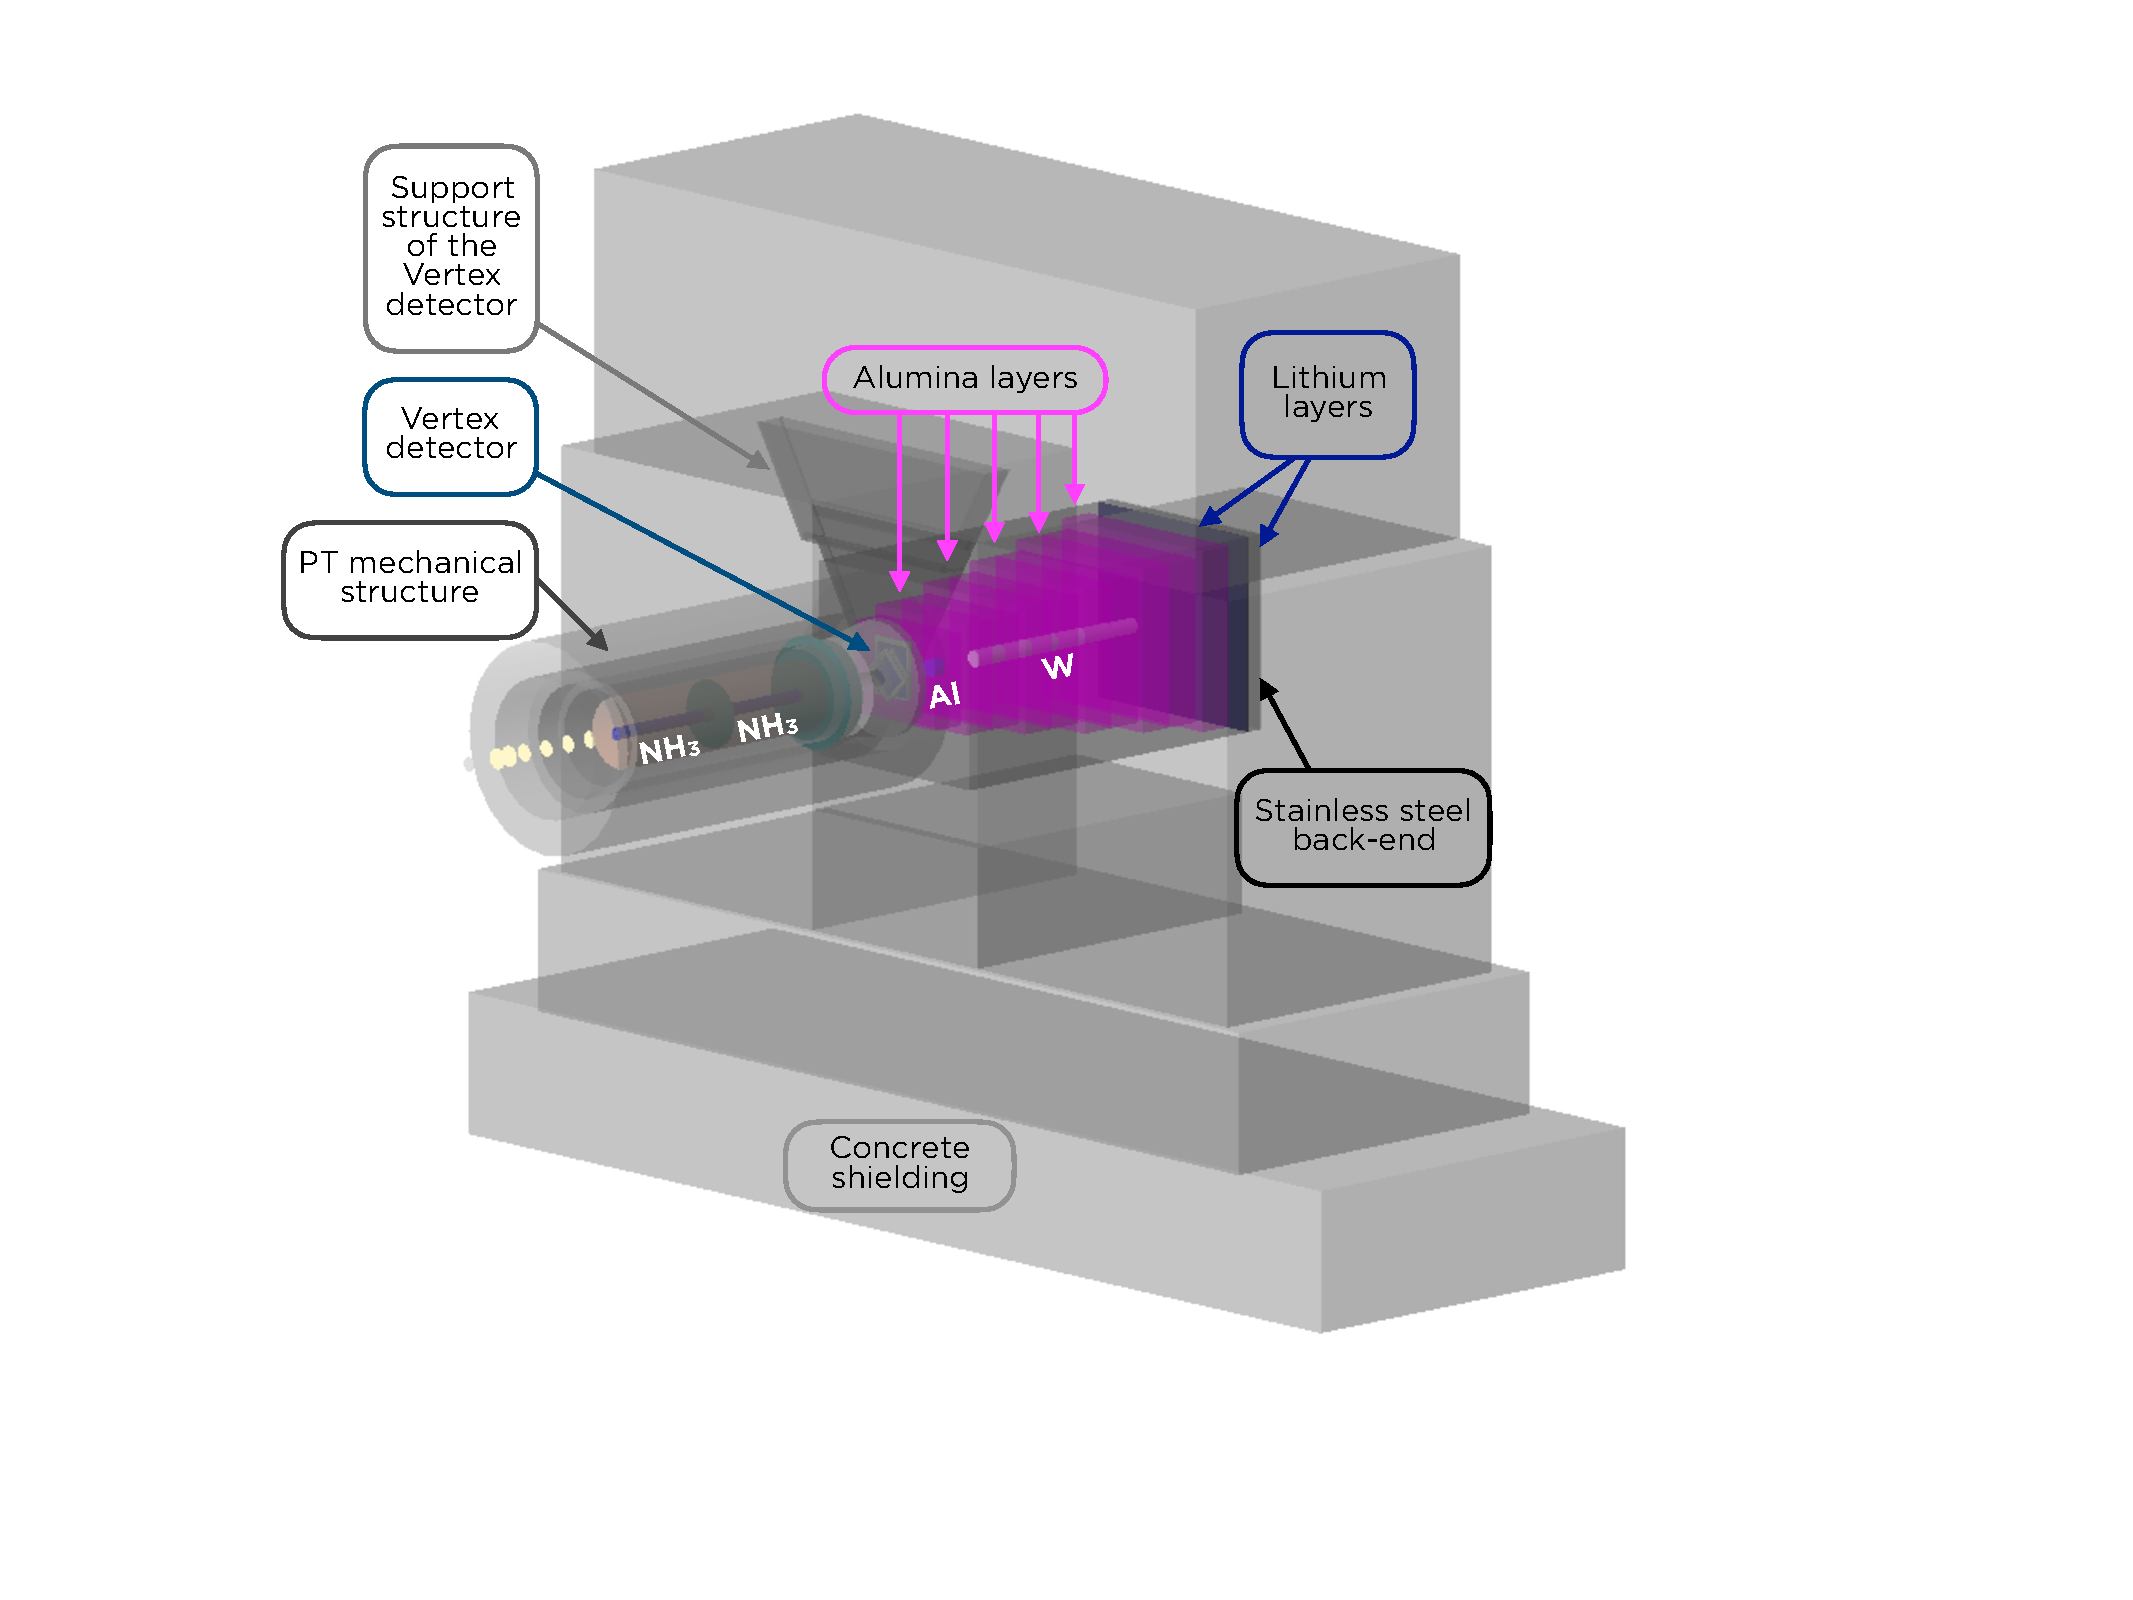
\includegraphics[width=0.6\textwidth]{Habs}
  \caption{The hadron absorber downstream of the polarized target in 2015.  This
    image was taken from~\cite{longothesis}.}
  \label{fig::Habs}
\end{figure}

\begin{figure}[h!t]
  \centering
  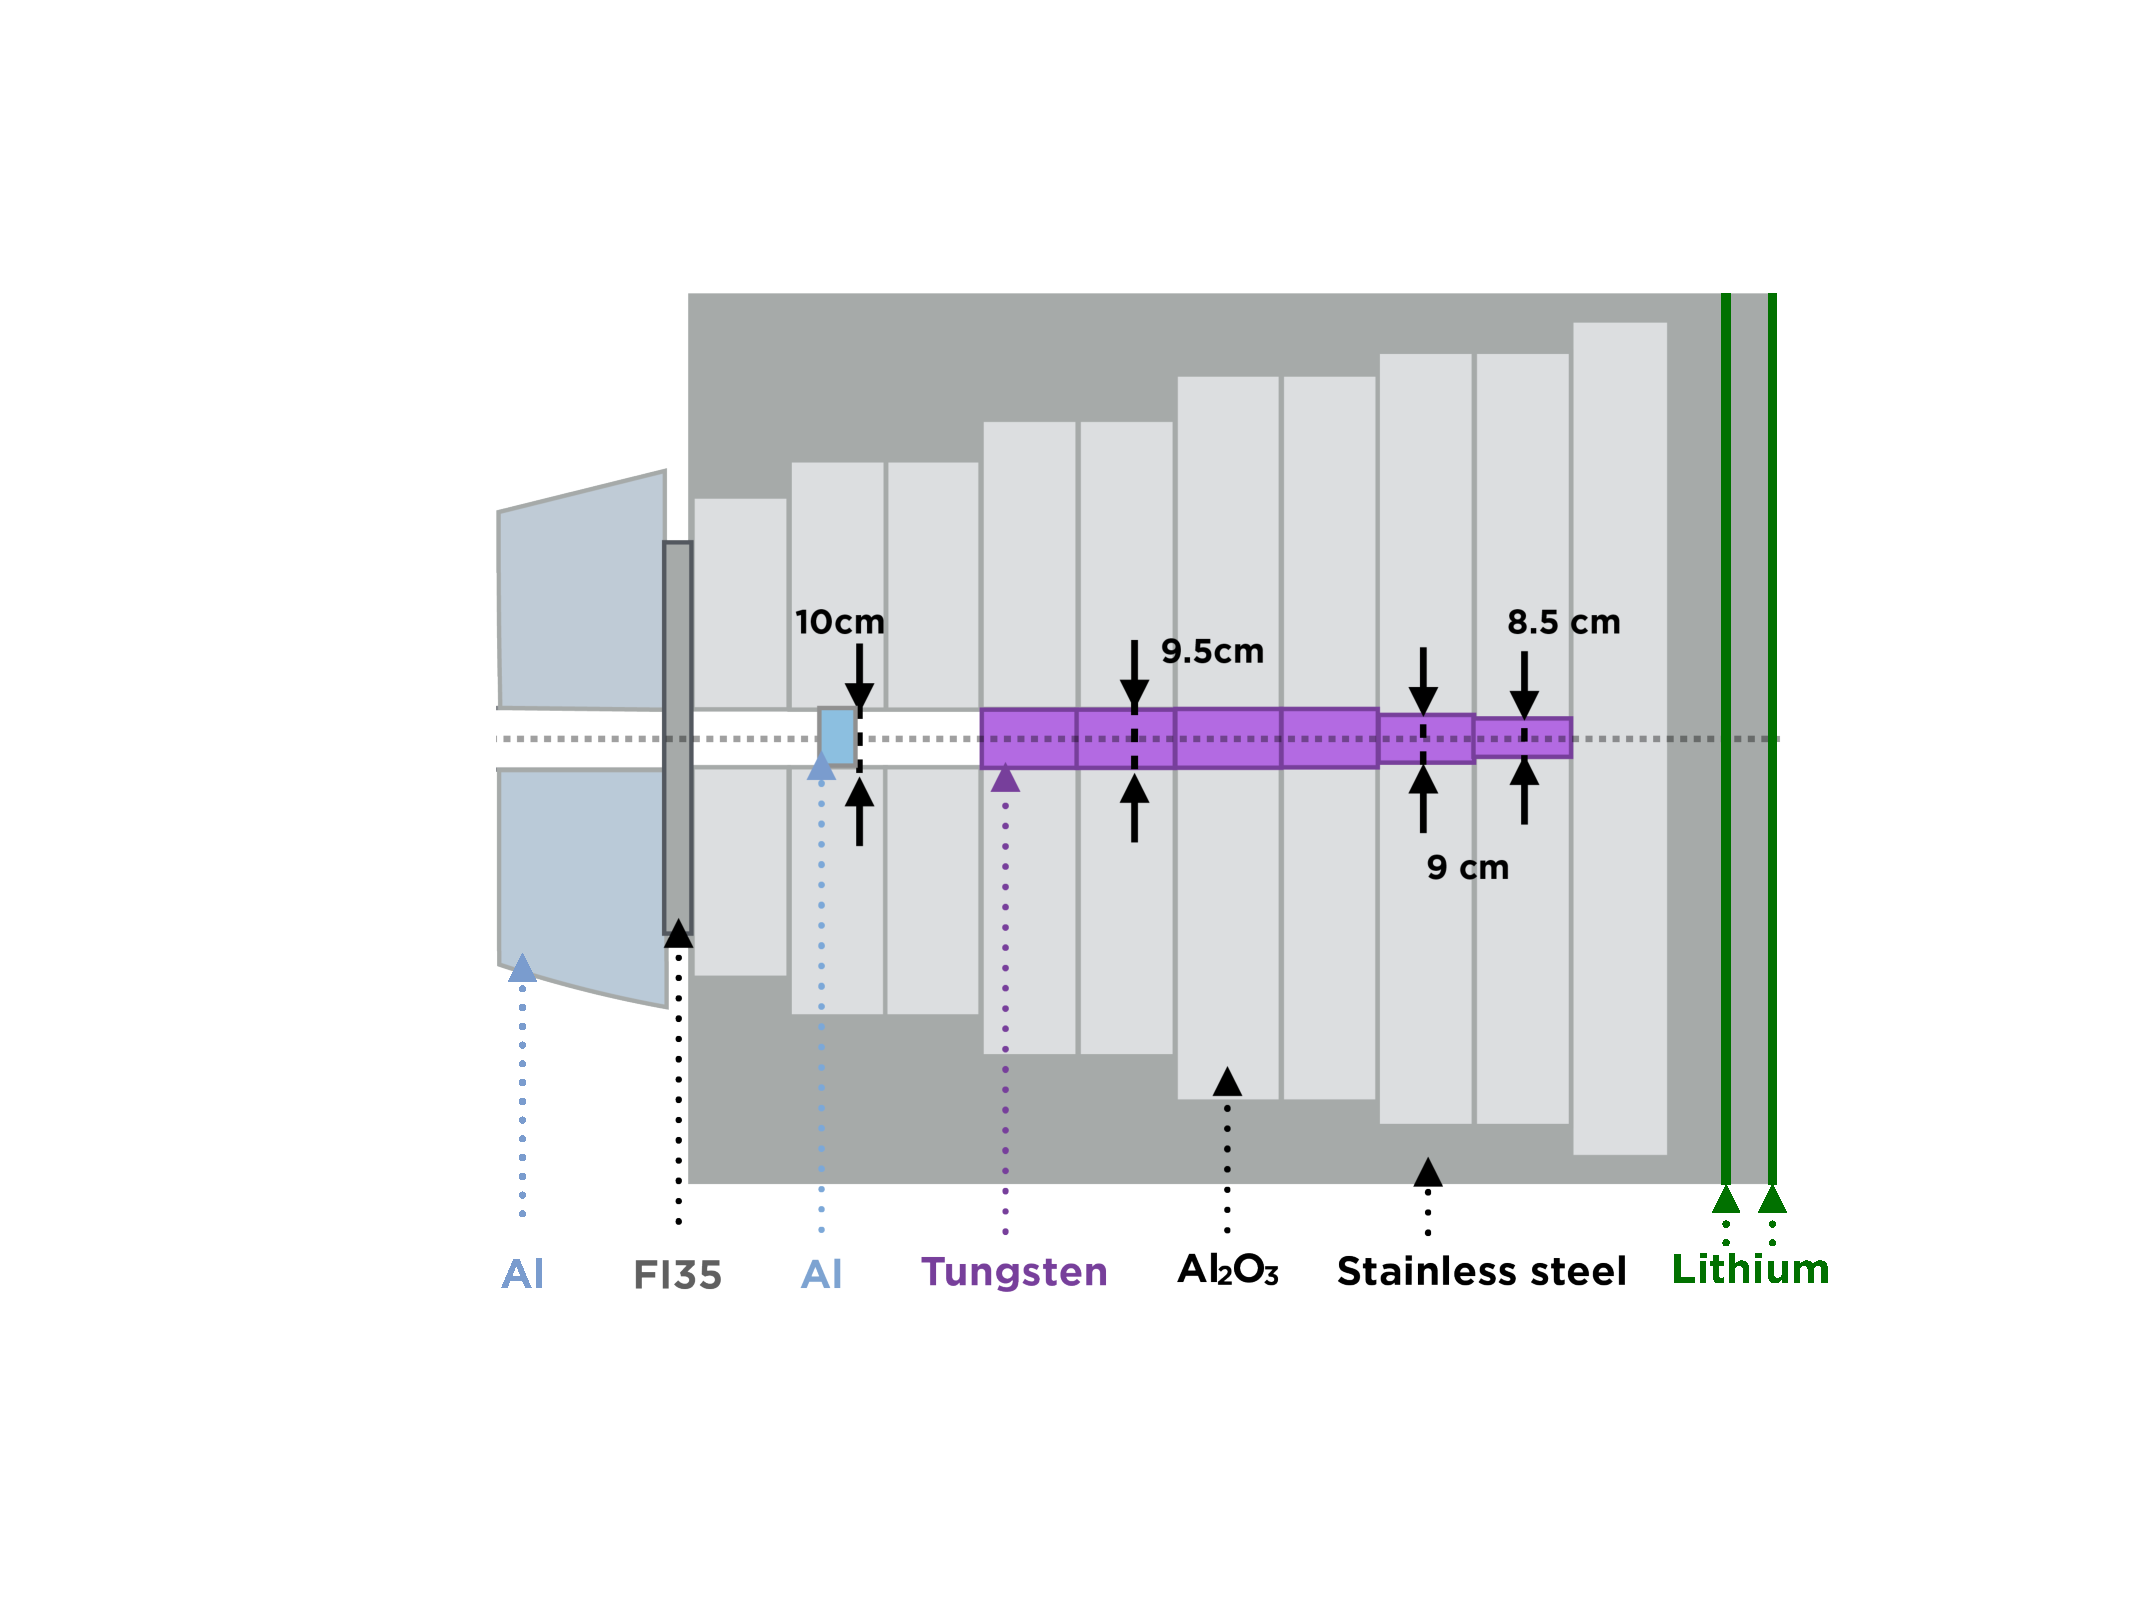
\includegraphics[width=0.6\textwidth]{Abside}
  \caption{Side view of the hadron absorber used in 2015.  This image was taken
    from~\cite{longothesis}.}
  \label{fig::Abside}
\end{figure}

%\chapter{Drift Chamber 05} \label{ch::dc05}
\ifpdf
\graphicspath{{Chapters/DC5/Figs/Raster/}{Chapters/DC5/Figs/PDF/}{Chapters/DC5/Figs/}}
\else \graphicspath{{Chapters/DC5/Figs/Vector/}{Chapters/DC5/Figs/}}
\fi

Drift Chamber 05 (DC05) is a large-area planar drift chamber.  It was
constructed in 2014 and 2015 at the University of Illinois and Old Dominion
University and was then shipped to CERN for final assemble.  DC5 was installed
to the large angle spectrometer of COMPASS during the spring of 2015.

The DC5 detector is an import tracking detector, which successfully collected
data from 2015 through 2018 and will continue to be an important component for
track reconstruction in future measurements.  The author of this thesis helped
with the construction at Illinois and the assembly at CERN and as well for
performing calibrations and maintaining DC5.


\section{Motivation for Drift Chamber 05}

Simulations of the COMPASS spectrometer for Drell-Yan measurements determined
that 96\% of all events include a track in the large angle
spectrometer~\cite{proposal}.  For this reason the Drell-Yan trigger system was
designed only to record events with at least one track in LAS.  As DC5 was
installed in LAS it is therefore very important in track reconstruction for
Drell-Yan measurements.  Additional simulations with the Drell-Yan setup and
this corresponding COMPASS Drell-Yan trigger showed that the global
reconstruction efficiency drops below 30\% without DC5 and half of another large
area tracker in LAS~\cite{quintans_rec_march12}.  That is to say the
spectrometer reconstruction efficiency is very poor without DC05 and half of
another LAS large area trackers which has unstable performance.
Fig.~\ref{fig::standardRec} and Fig.~\ref{fig::withLARec} show the nominal
global reconstruction efficiency and the worst case scenario for Drell-Yan
measurements respectively.  For these reasons it was very important to have DC05
installed and working reliably.

\begin{figure}[h!t]
  \centering
  \begin{subfigure}{.5\textwidth}
    \centering 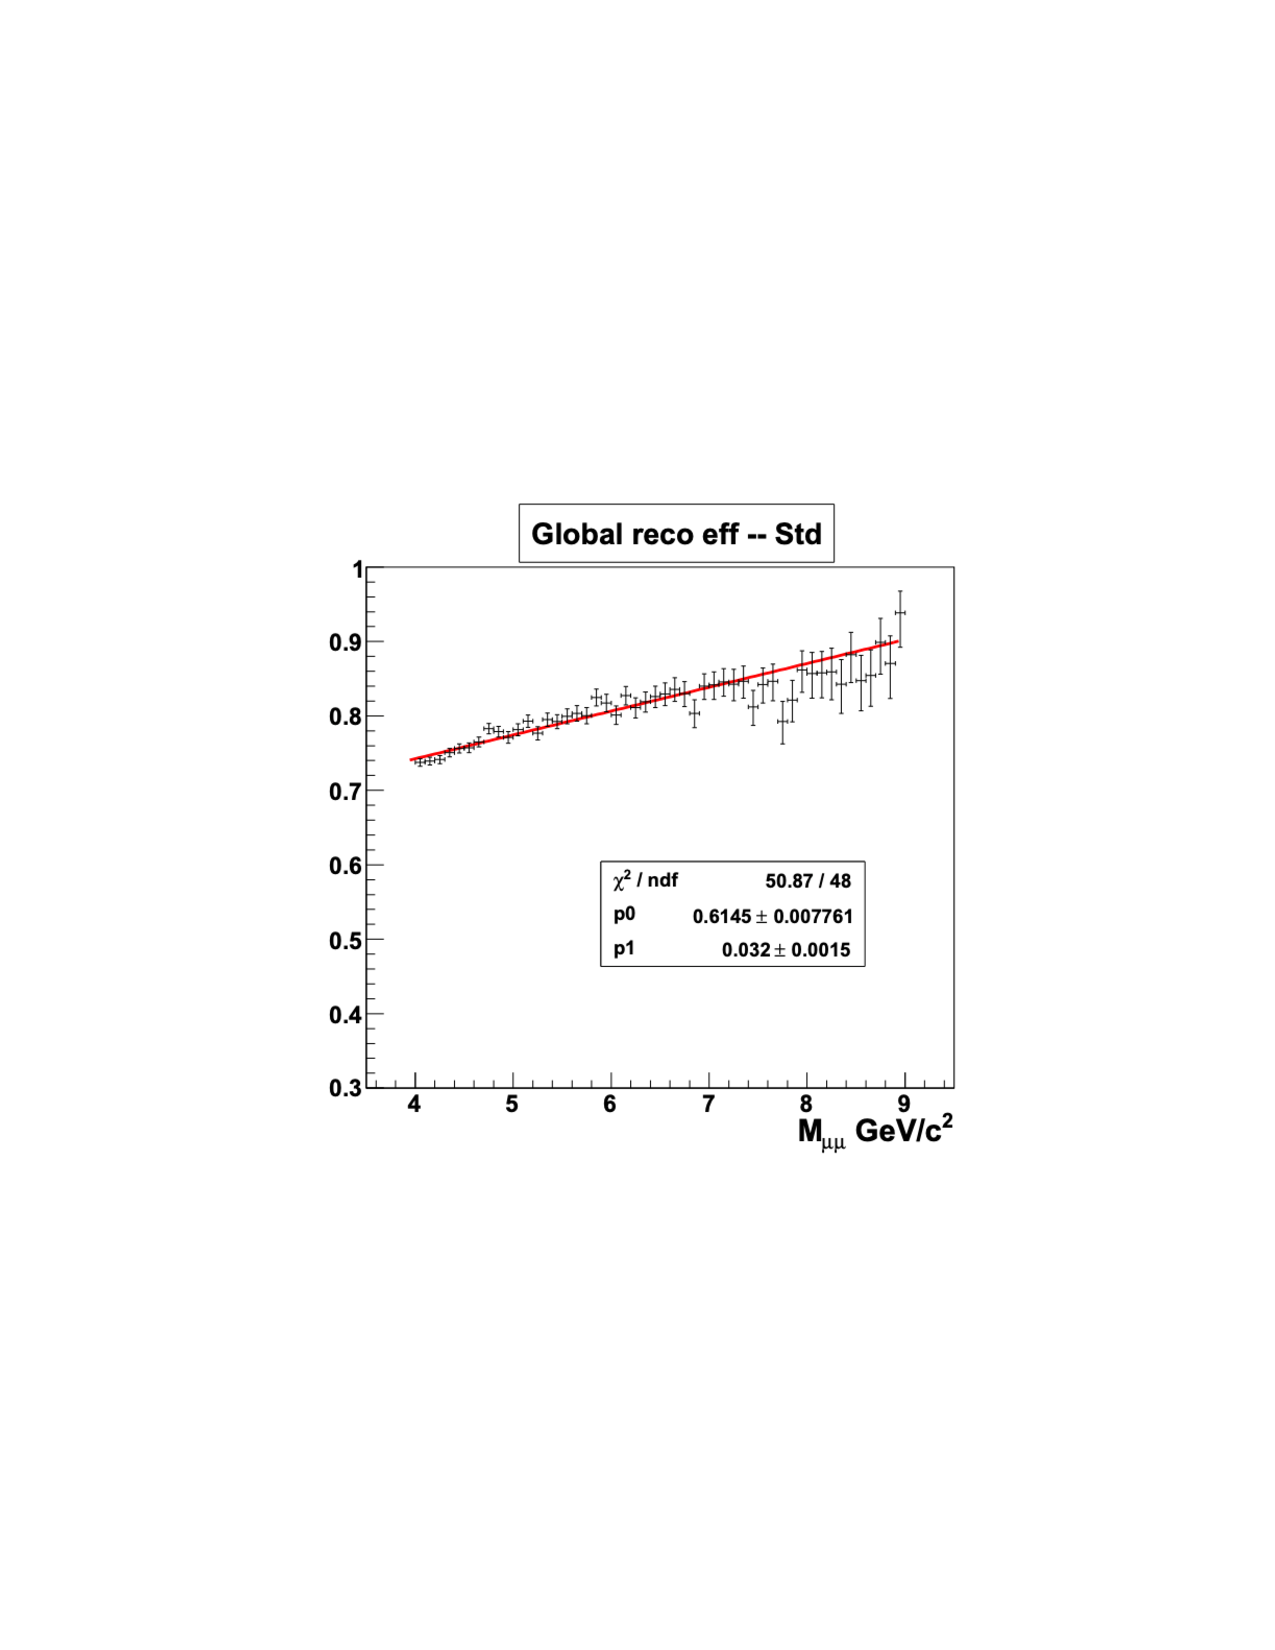
\includegraphics[width=\linewidth, trim=5cm 8cm 5cm 8cm,
      clip]{standardRec}
    \caption{Global reconstruction efficiency with all detectors working.  This
      image was taken from~\cite{quintans_rec_march28}}
    \label{fig::standardRec}
  \end{subfigure}%
  \begin{subfigure}{.5\textwidth}
    \centering
    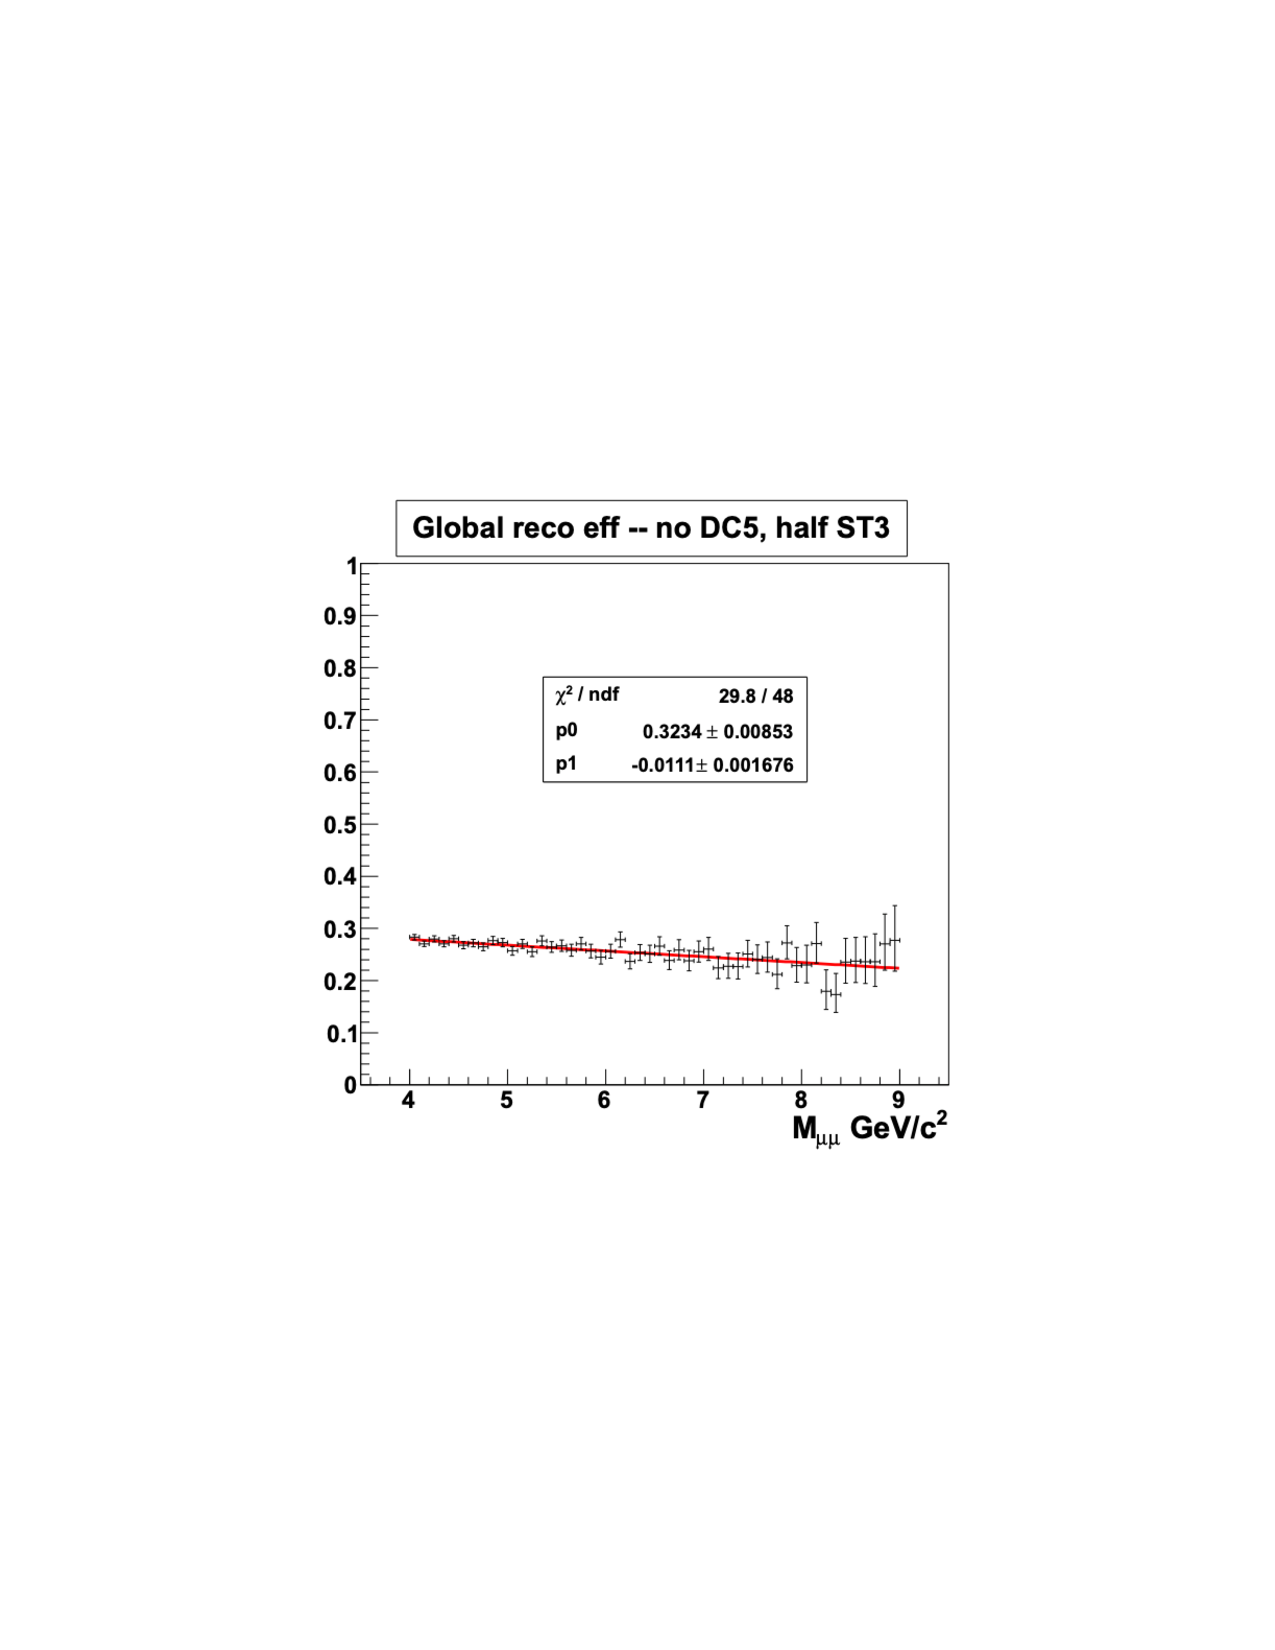
\includegraphics[width=\linewidth, trim=5cm 8cm 5cm 7.5cm, clip]{withLARec}
    \caption{Global reconstruction efficiency without DC05 and half of another
      LAS large area tracker.  This image was taken
      from~\cite{quintans_rec_march28}}
    \label{fig::withLARec}
  \end{subfigure}
\end{figure}


\section{Operating Principle}

Drift chambers are tracking detectors which can detect the location of where a
high energy charge particle passes through them.  A drift chamber is
built up of an array of drift cells where at the center of each drift cell is an
anode signal wire (also called a sense wire).  Surrounding the signal wire are
cathodes which close off the drift cell.  The cathodes are set at a higher high
voltage than the anode and therefore there are electric field lines from the
cathode to the anode.  Fig.~\ref{fig::dcCellFieldLines} shows an example of a
drift chamber cell and the equipotential voltages within the cell.  In DC05 the
there are two cathode planes on top and bottom of the drift cell and a cathode
field wire adjacent to either side of the sense wire.

\begin{figure}[h!t]
  \centering
  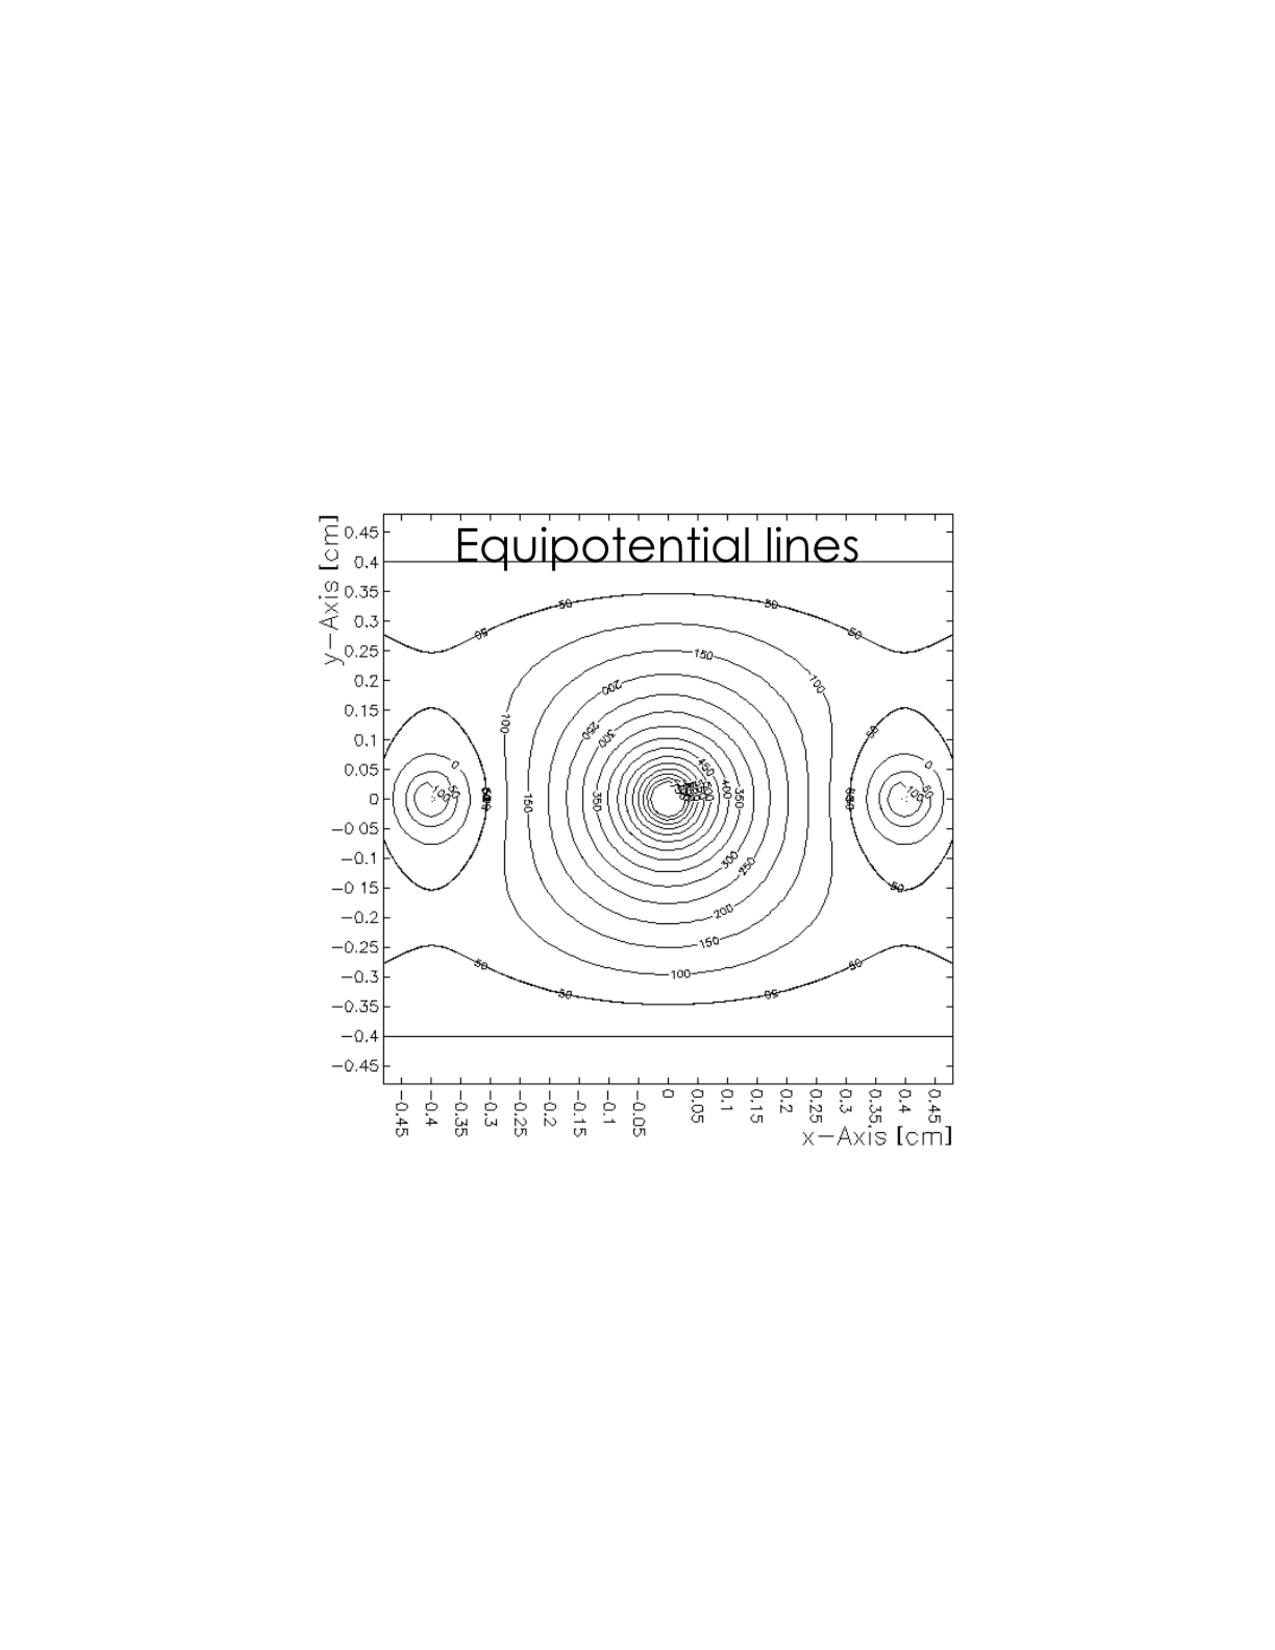
\includegraphics[width=0.6\textwidth, trim=4.5cm 8cm 4.5cm 8cm, clip]
                  {dcCellFieldLines}
  \caption{View down the axis of a drift cell and the equal voltages for this
    drift cell configuration.  This image is taken from~\cite{ran_bi}}
  \label{fig::dcCellFieldLines}
\end{figure}

Between the anodes and cathodes of a drift cell is a gas mixture.  The high
energy charged particles which enter the chamber ionize this gas mixture.  For
each track passing through the chamber, multiple primary ionization electrons
are produced and these electrons drift to the signal wire.  The number of
primary ionization electrons produced however, is not enough to create a
detectable signal on the sense wires.  For this reason the electric field
increases as the inverse of the distance from the sense wire which allows the
primary ionization electrons to gain enough energy to further ionize the gas and
ultimately produce an electron avalanche near the sense wire.  The signal
created from this electron avalanche is strong enough to detect.  A typical
detector is built so that an avalanche can occur before the sense wire but not
before a cathode wire.  This is accomplished by constructing the chamber with
sense wires having a much smaller diameter than the field wires, meaning the
electric field near the sense wire can be much larger than the electric field
near the field wire.

An important factor for a drift chamber is that the location of the primary
ionized electrons can be determined within a drift cell.  This knowledge allows
for a better position determination of the passing track as compared to a
multi-wire proportional chamber.  Each sense wire records the time a signal was
detected from a track.  For the same track, the trigger records the time the
track enter the drift chamber and therefore the difference in time between the
sense wire time and the trigger time is the drift time.  For a drift chamber it
is possible to produce a calibration curve which determines the position within
a drift cell for a given drift time.  This calibration curve is so-called the RT
relation.

Even with a properly calibrated RT relation the track location is ambiguous from
only one drift cell.  This is because a single drift cell can only determine a
track location as a distance from the sense wire.  Therefore it is ambiguous
where along the sense wire the track passed and also if the track passed to the
left or right of the sense wire.  For this reason drift chambers are built with
several planes in series.  A drift cell with the same orientation but shifted
with respect to the first drift cell is used to distinguish left and right
ambiguity and another cell with an orientation at an angle with respect to the
first is used to determined where along the wire the track passed.


\section{Preparation for DC05}

One of the first steps in preparation for constructing DC05 was to simulate the
detector response using Garfield~\cite{garfield}.  The purpose of these
simulations was to determine an operating threshold capable of achieving a
200~$\mu$m position resolution.  With this position resolution goal in mind,
Garfield simulated the electric potential field in each drift cell, as shown in
Fig.~\ref{fig::dcCellFieldLines}, and was able to determine the arrival times
for ionized electrons as a function of the number of primary ionized electrons
for detection.  This is important because the timing distribution for electron
arrival times gets wider and therefore worsens the position knowledge as the
number of primary electrons required for a signal increases.  The variance of
the electron arrival times was then used to determine the position resolution as
a function of the number of primary electrons needed for detection.  As is shown
in Fig~\ref{fig::PosResVnumElec}, the threshold should be tuned to detect the
amplification of the fifth primary electron~\cite{ran_bi}.  As is shown in
Fig.~\ref{fig::currentVtimeFifthElec} based on the simulation of the integrated
induced current versus the drift arrival time, the threshold for detecting the
signal should be no greater than 4~fC~\cite{ran_bi}.  This threshold charge is
determined by multiplying the induced current by the arrival time.  The
threshold was accordingly one of the design goals for the front-end electronics.

\begin{figure}[h!t]
  \centering
  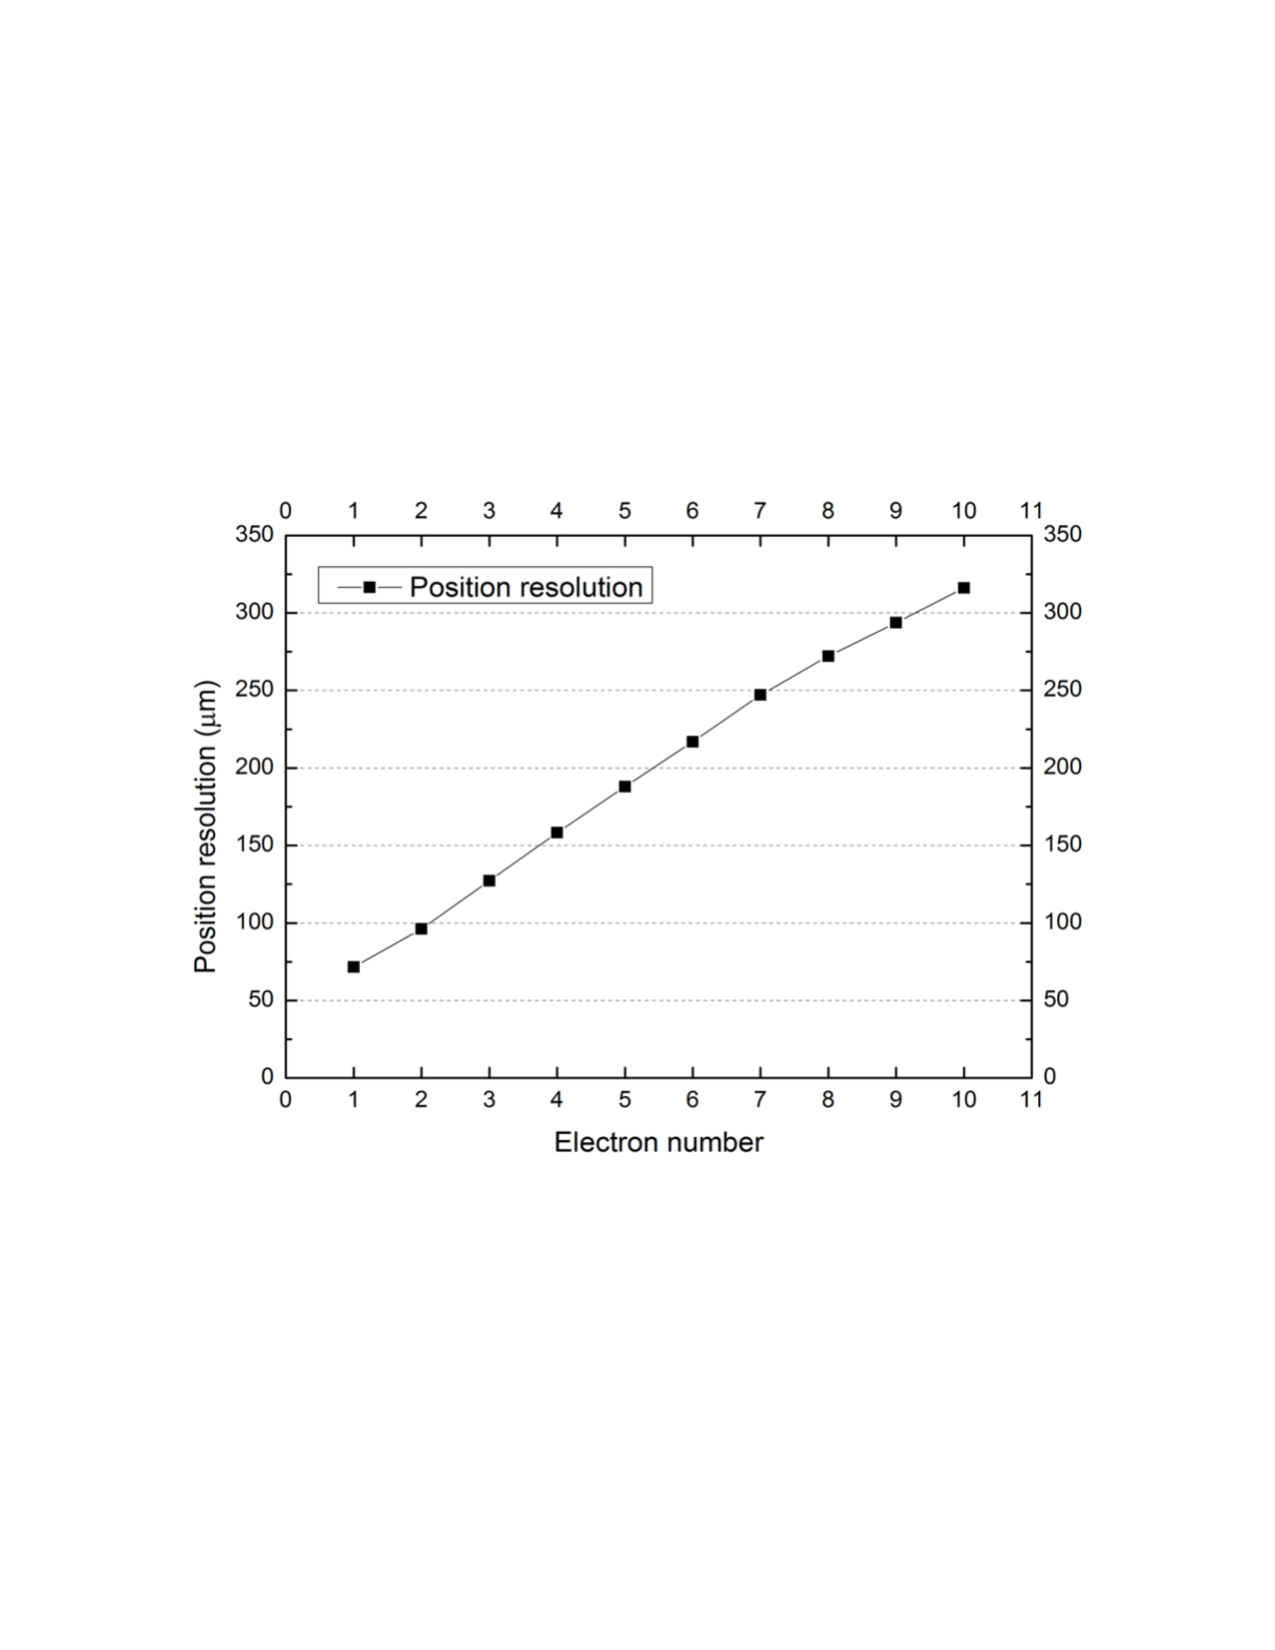
\includegraphics[width=0.55\textwidth, trim=3cm 8cm 3cm 8cm, clip]
                  {PosResVnumElec}
  \caption{A simulation of the position resolution as a function of the number
    of primary electrons needed to record a signal.  This image is taken
    from~\cite{ran_bi}}
  \label{fig::PosResVnumElec}
\end{figure}

\begin{figure}[h!t]
  \centering
  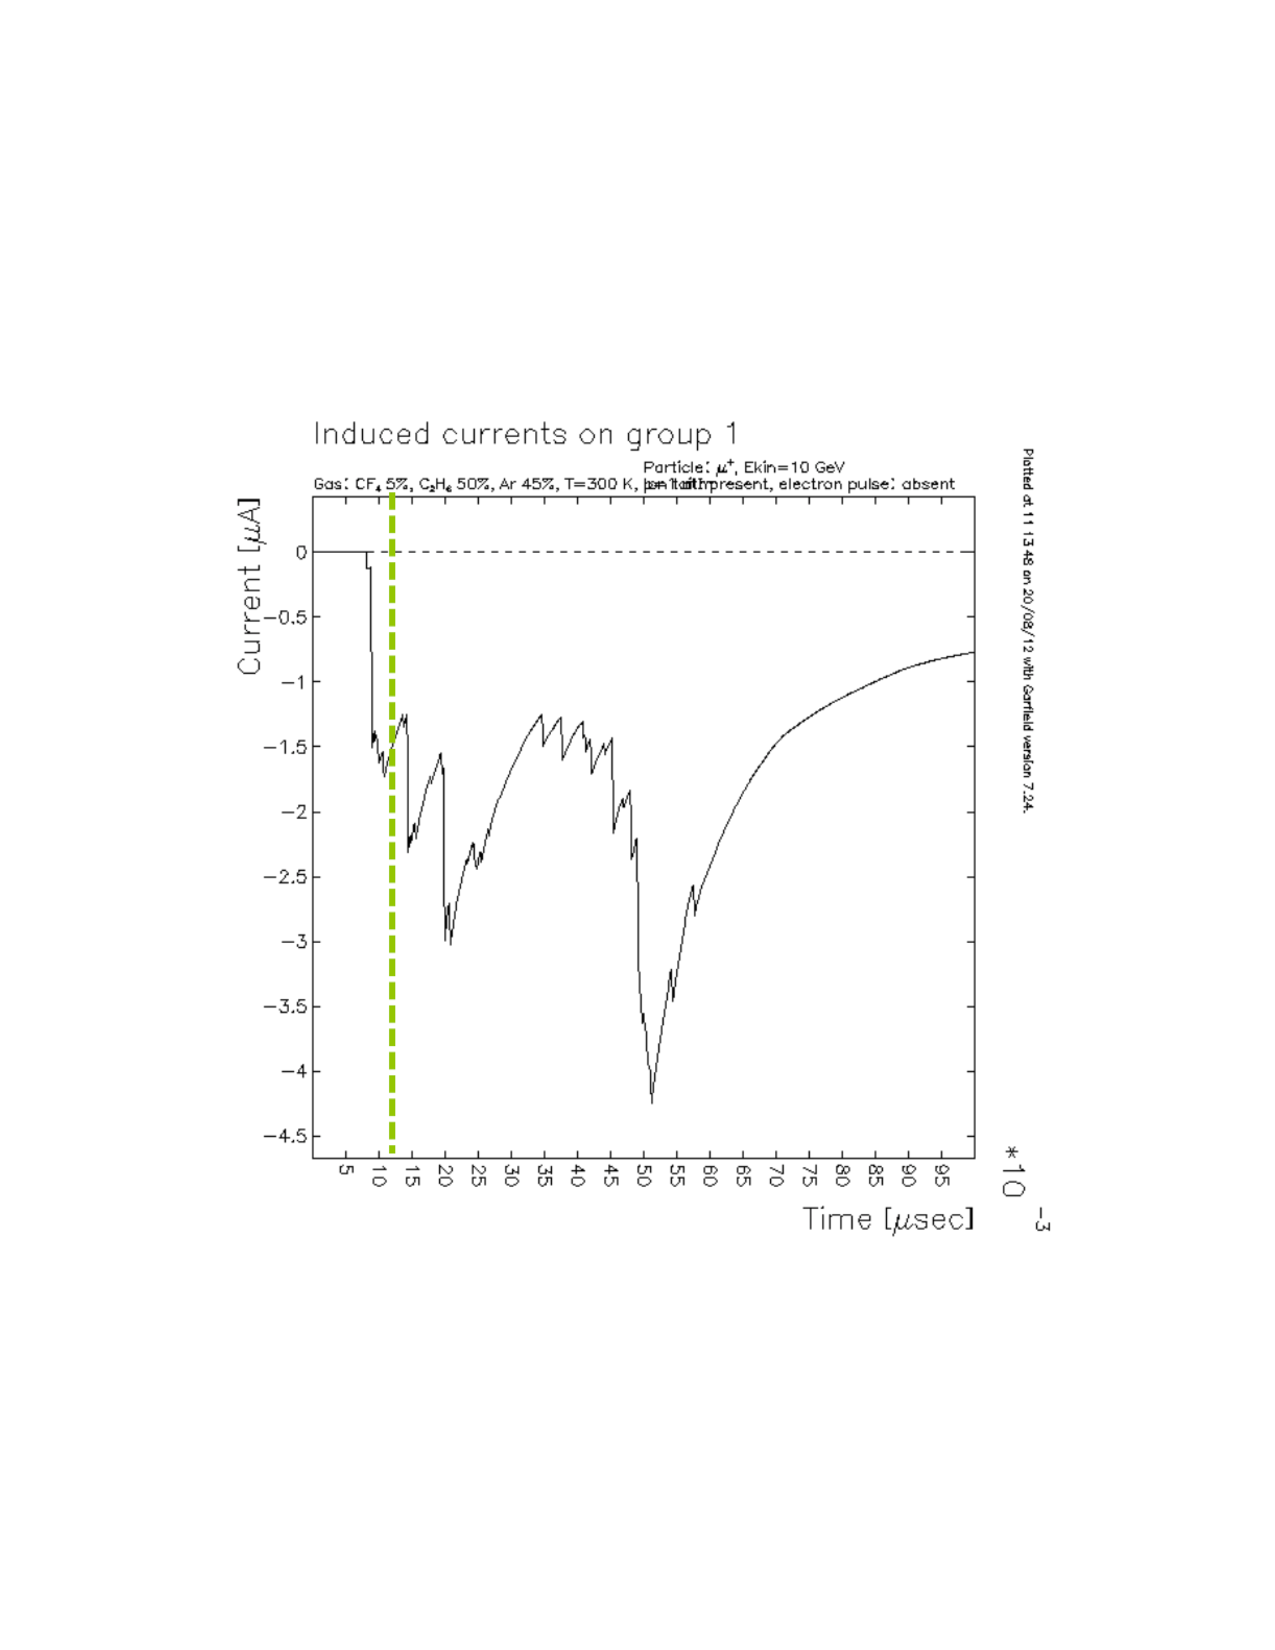
\includegraphics[width=0.55\textwidth, trim=3cm 6cm 3cm 6cm, clip]
                  {currentVtimeFifthElec}
  \caption{Garfield simulation of the induced signal current versus the arrival
    time.  The green line corresponds to the arrival time of the fifth election.
    This image is taken from~\cite{ran_bi}}
  \label{fig::currentVtimeFifthElec}
\end{figure}

Two prototypes were built to gain hands on building expertise in preparation for
construction.  Both of these prototypes were constructed in a clean room in the
Nuclear Physics Lab (NPL) at UIUC.  Much of DC05 was built at the NPL as well.
The two prototypes were called prototype A and prototype B.  Prototype A,
Fig.~\ref{fig::protoTypeA}, consisted of 1 plane, eight sense wires, 9 field
wires and was 50~cm in length.  Prototype B on the other hand consisted of two
planes with 16 sense wires per plane and a length of 163~cm.  Prototype A was
tested with beam at DESY and was shown to achieve 200~$\mu$m
resolution~\cite{choi}.  Both of these prototypes were built using similar
materials and construction techniques as the full size detector.  In particular
these two prototypes were the needed experience for working with sense wires
having a diameter of 20~$\mu$m.

\begin{figure}[h!t]
  \centering 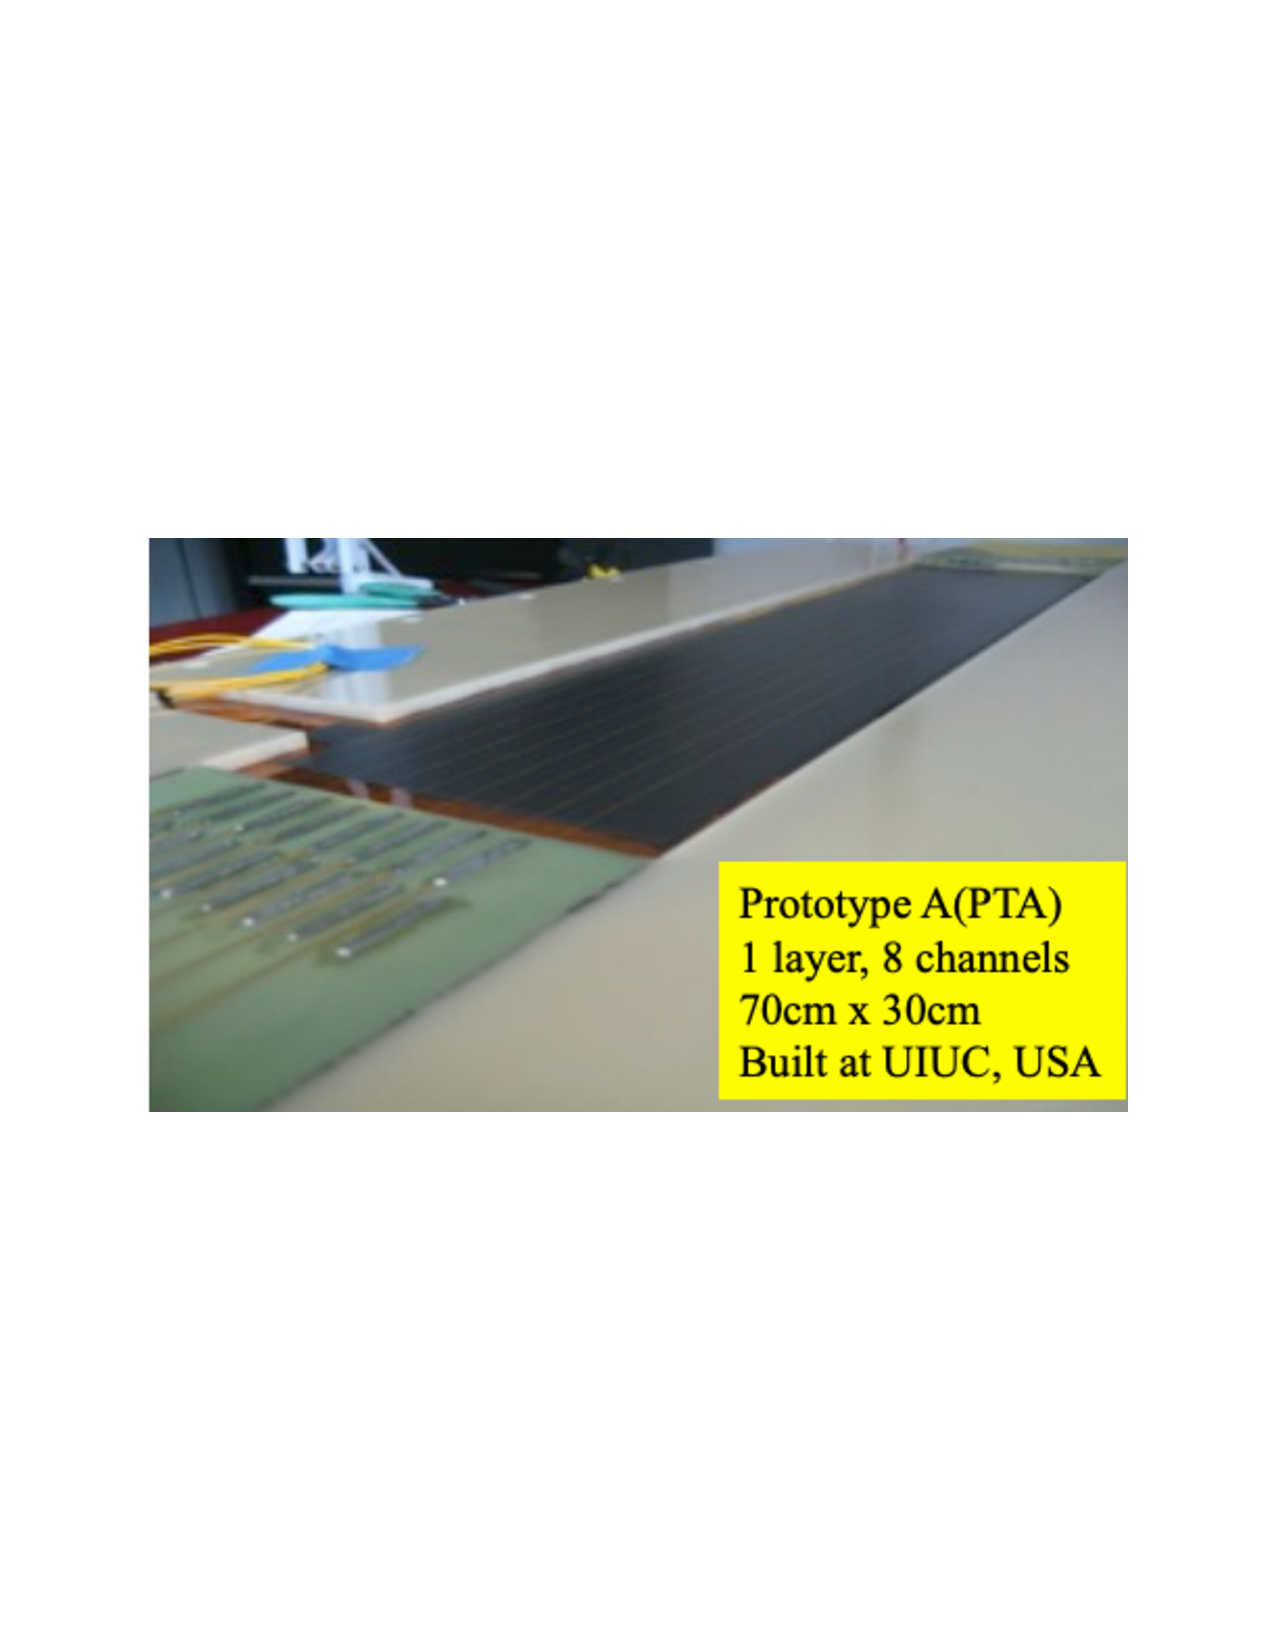
\includegraphics[width=0.6\textwidth, trim=2.5cm 8cm 2.5cm 8cm,
    clip]{protoTypeA}
  \caption{Inside view of prototype A.  This image was taken from~\cite{choi} }
  \label{fig::protoTypeA}
\end{figure}


\section{Design}

\begin{figure}
  \centering 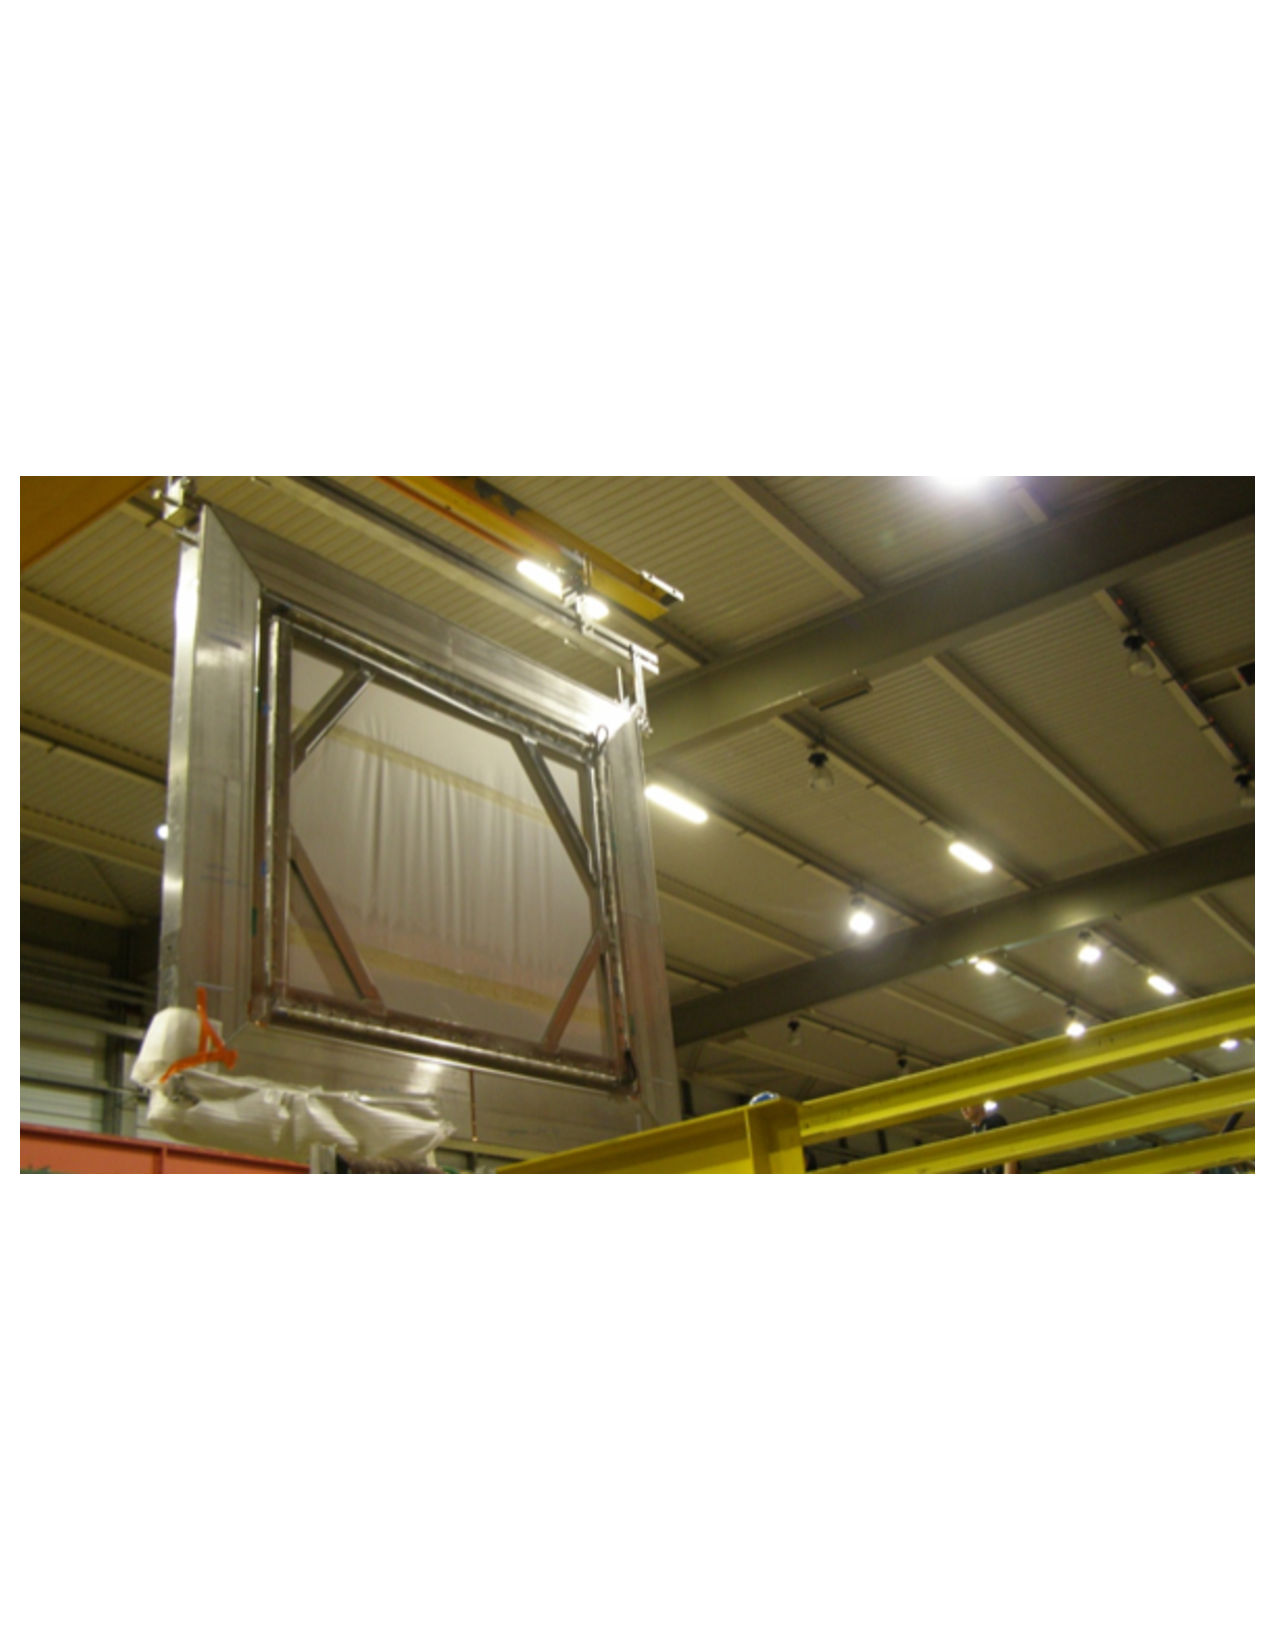
\includegraphics[width=0.7\textwidth, trim=2.5cm 8cm 2.5cm 8cm,
    clip]{DC05_full}
  \caption{}{The completed DC05 being craned into the COMPASS large area
    spectrometer.}
  \label{fig:DC05}%
\end{figure}

The design of DC05, figure~\ref{fig:DC05}, was based off a previous large-area
tracker at COMPASS.  DC05 has an active area of 249x209cm$^2$ and consists of
eight detector planes.  The eight planes of DC05 correspond to four views, where
each view measures a coordinate.  The coordinates measured from DC05 are the
horizontal, vertical and $\pm$ 10$^{\circ}$ with respect to the horizontal.  The
horizontal and vertical coordinates consist of 2x256 sense wires and the offset
to horizontal coordinates each consist of 2x320 wires for increased acceptance.
In total DC05 includes 2304 sense wires and 2312 field wires.  Each plane was
made from a G-10 frame and five frames stacked together constituting a view.
The whole detector was closed in with two precision, stainless steel stiffening
frames, which were assembled with aluminized mylar as a gas window.

The views of DC05 consist of three cathode layers and two anode layers.  The
cathodes layers were made from carbon paint sprayed on a 25~$\mu$m thin mylar
layer.  There were two single-layer cathodes layers and one layer with carbon on
two sides within each view.  Fig.~\ref{fig::DC05_layers} shows a side view of
the layers of DC05.  Additionally a 30~cm circular so-called beam killer was
added to the cathodes to control the efficiency in the central part of the
detector.  The cathodes were nominally set to -1675~V and the beam killer
voltage was set to -900~V for zero efficiency in the high flux central region.
The voltage on the beam killer can however be raised above the amplification
threshold if the beam flux is reduced and it is desirable to study the central
region.

\begin{figure}[h!t]
  \centering 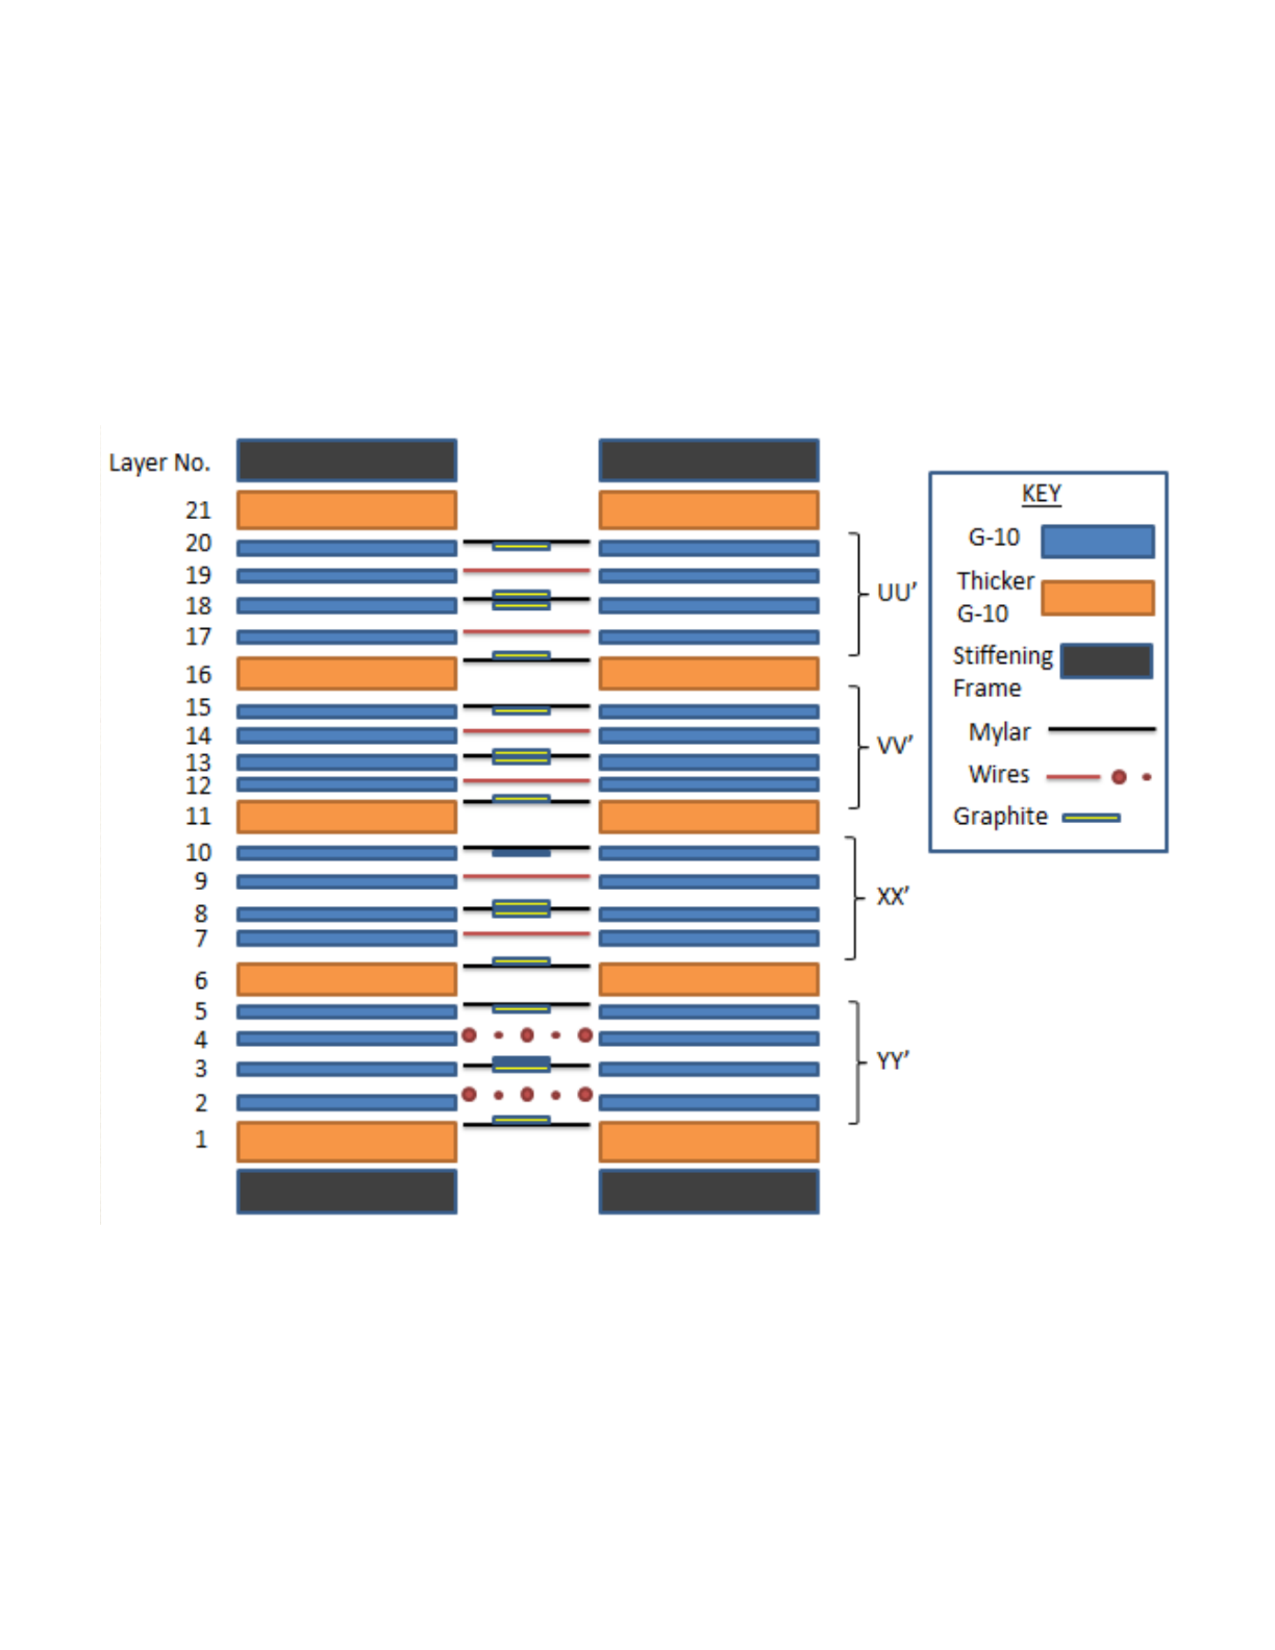
\includegraphics[width=0.7\textwidth, trim=0.2cm 7cm 0.2cm 2cm,
    clip]{DC05_layers}
  \caption{A side view sketch of the layers in DC05}
  \label{fig::DC05_layers}
\end{figure}

The anode layers were made from alternating 20~$\mu$m gold-plated tungsten sense
wires and 100~$\mu$m gold-plated copper beryllium field wires, as depicted in
figure~\ref{fig:driftcell}.  Gold plating was used for both sense and field
wires to prevent aging effects.  The field wires were also placed at -1675~V and
the sense wires were at 0~V.  The nominal gain of DC05 is approximately 10$^4$.

\begin{figure}
  \centering 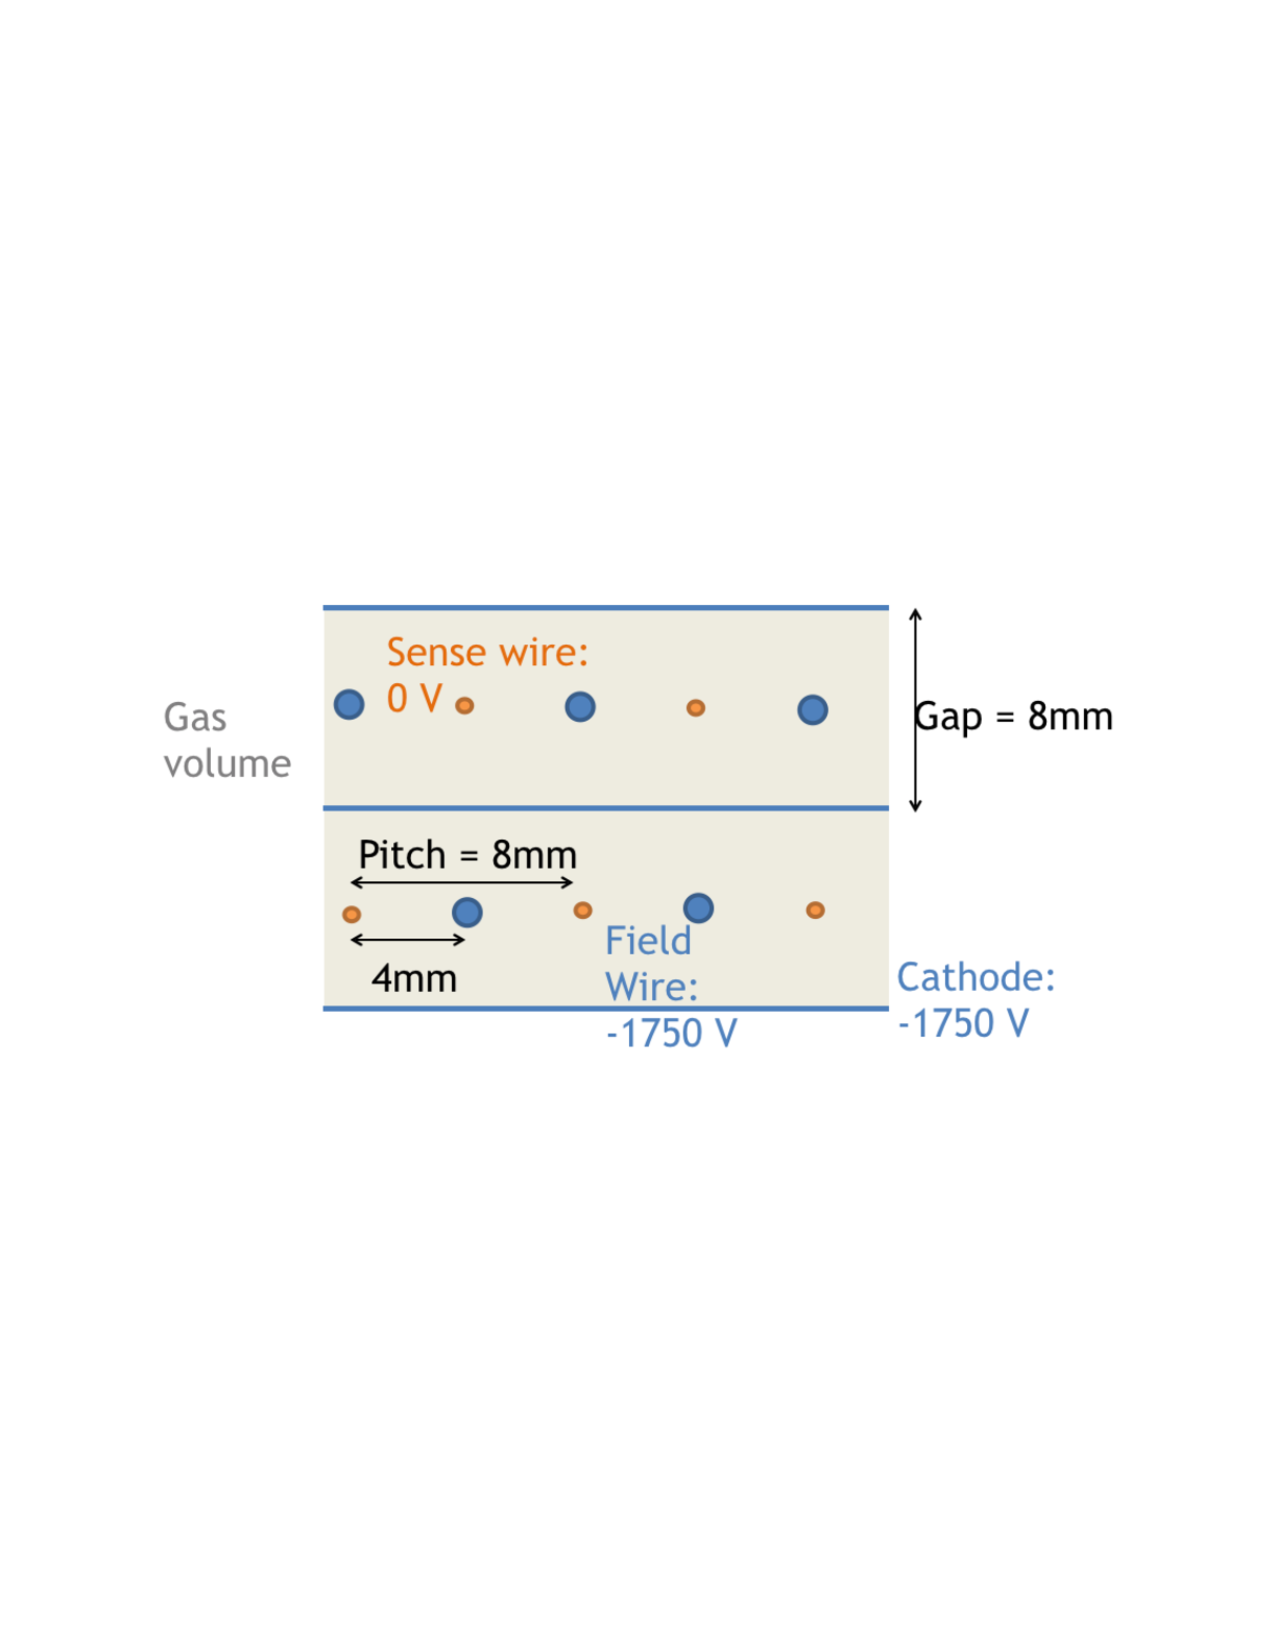
\includegraphics[width=0.5\textwidth, trim=2.5cm 10cm 3cm 10cm,
    clip]{DriftCell}
  \caption{}{The drift cell dimensions of one plane in DC05}
  \label{fig:driftcell}%
\end{figure}

During data taking, DC05 is filled with a mixture 45\% argon, 45\% ethane and
10\% Cf$_4$.  The noble gas, argon, is the gas that is ionized and amplified,
while ethane is used as a quencher and CF$_4$ is used to reduce aging effects.
The quencher, ethane, absorbs photons from the electron avalanche which could
pair produce and therefore make more electrons which would distort the electric
field in a drift cell.  The quencher therefore is used to reduce the avalanche
and ensure the drift cell electric field lines are closer to their design values.  


\section{Construction}

The construction of DC05 was carried out as precisely as possible starting with
the precision from the stainless steel stiffening frames.  The stiffening frames
where cut with the highest relative accuracy by cutting the two frames on top of
each other to a precision of 50~$\mu$m everywhere in their plane.  The precision
from the stiffening frames was transferred to the anode and cathode frames
through 40 positioning pins.  The G-10 frames were milled from strips at the NPL
using a precision milling machine.  Each four strips were then epoxied together
on top of one of the stiffening frames.

The cathodes had mylar stretched and epoxied to them using a custom built
stretching machine at CERN.  Fig.~\ref{fig::mylarStretching} shows the process
of stretching mylar on a cathode.  An external company then spray painted carbon
on them which was then polished till the resistance was approximately
30~k$\Omega /m$.  All the sense and field wires were hand soldered as shown in
Fig.~\ref{fig::wireSoldering}, and sequentially verified for position using a
microscope.  It was estimated the position placement of each sense wire was at
least as good as half the diameter of a sense wire or precise to 10~$\mu$m.

\begin{figure}[h!t]
  \centering 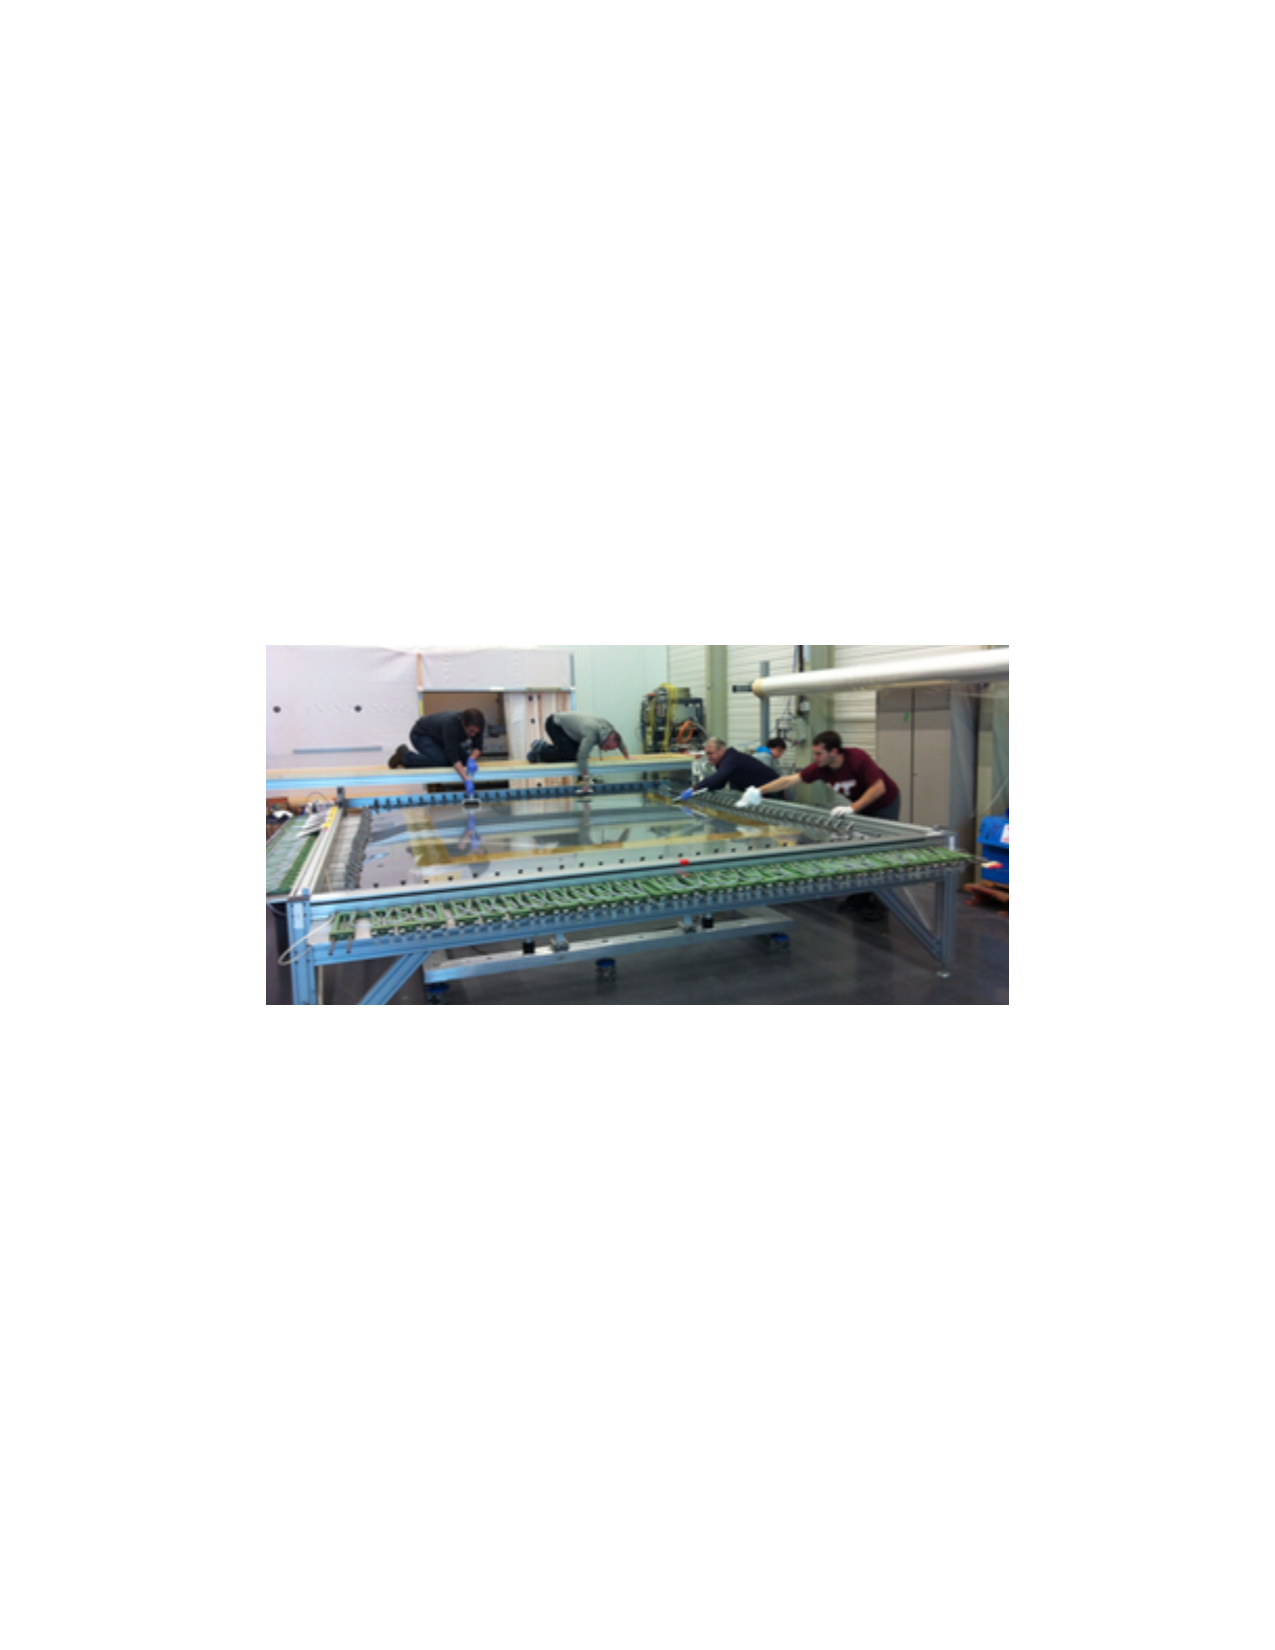
\includegraphics[width=0.6\textwidth, trim=5cm 12cm 5cm 10cm,
    clip]{mylarStretching}
  \caption{Stretching mylar on a cathode plane at CERN}
  \label{fig::mylarStretching}
\end{figure}

\begin{figure}[h!t]
  \centering 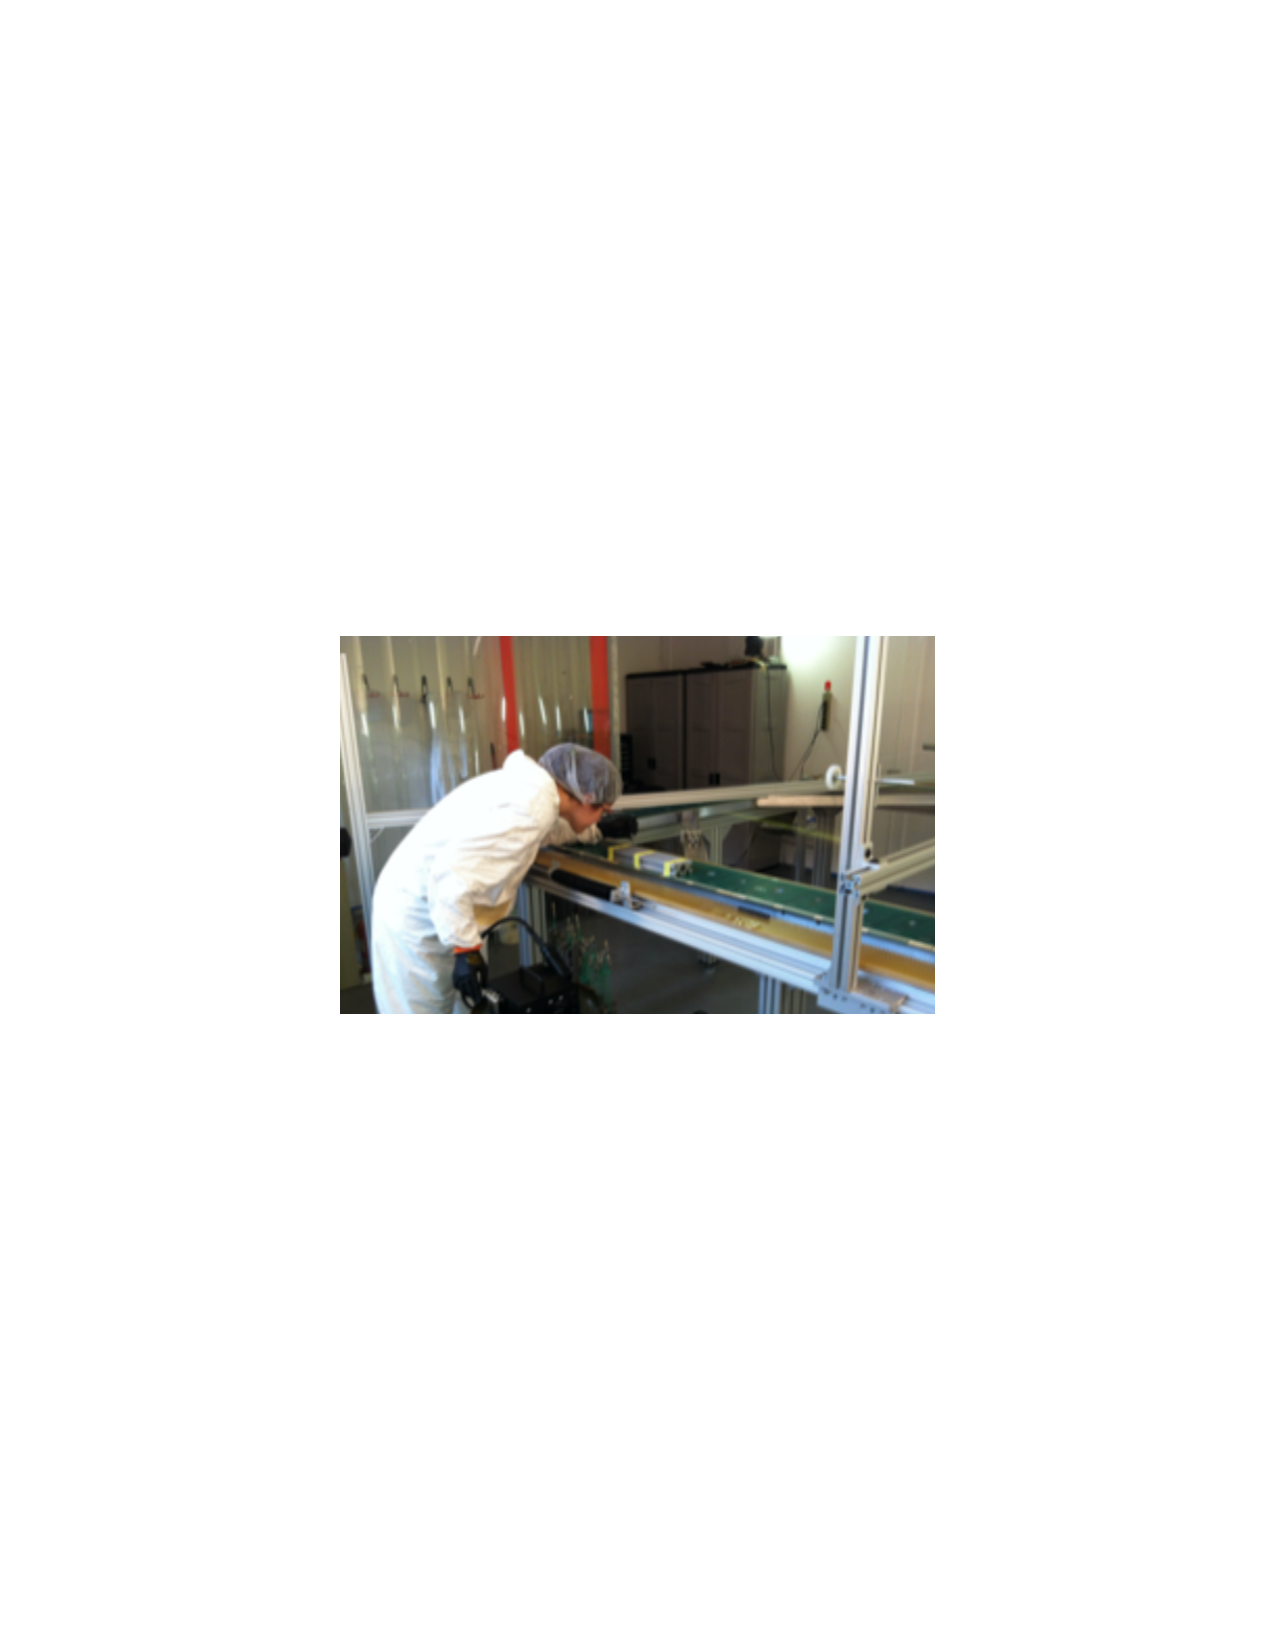
\includegraphics[width=0.6\textwidth, trim=5cm 10cm 5cm 10cm,
    clip]{wireSoldering}
  \caption{Hand soldering DC05 wires in the clean room at the NPL}
  \label{fig::wireSoldering}
\end{figure}

The final assemble was done at CERN.  This consisted of stacking each of the 21
G-10 frames on top of the stiffening frame, Fig.~\ref{fig::cernFinalAssembly},
and attaching copper electronic shielding all along the exterior of the detector
to reduce electronic noise.

\begin{figure}[h!t]
  \centering 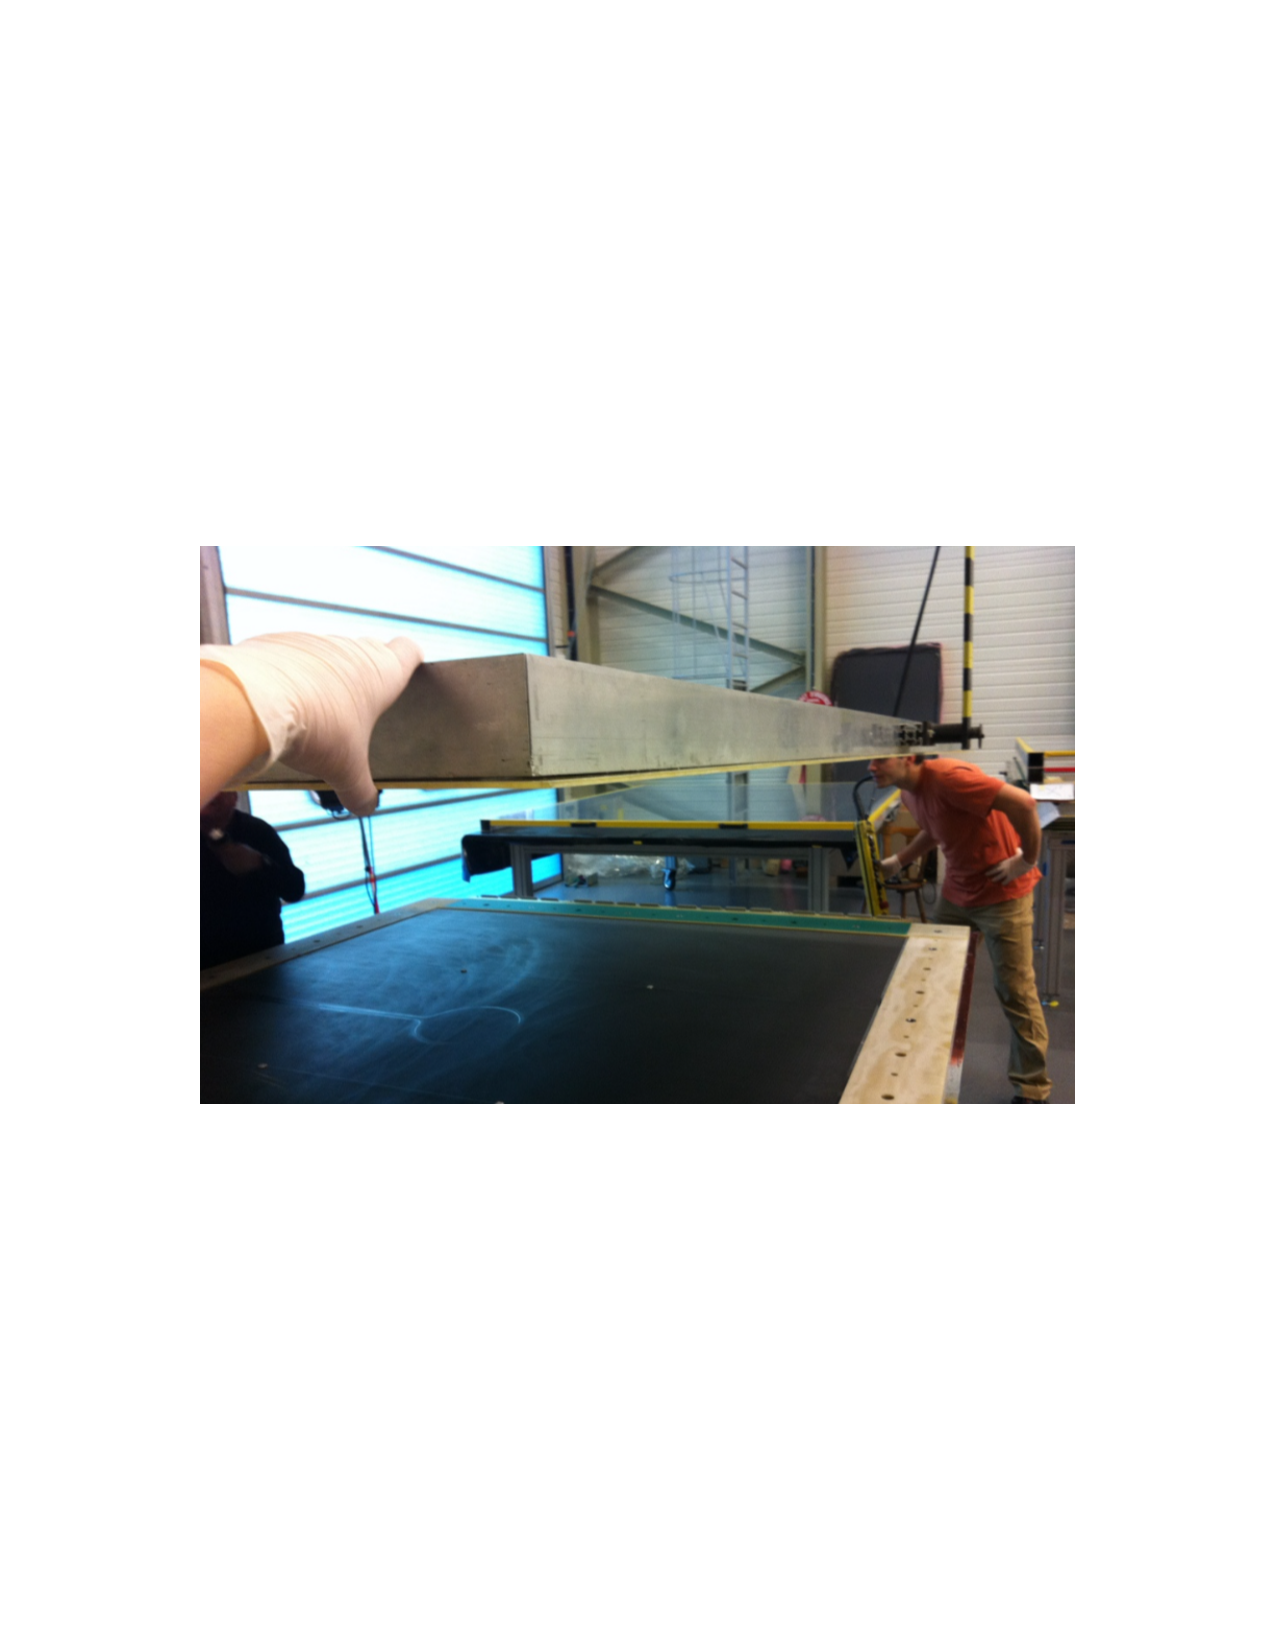
\includegraphics[width=0.6\textwidth, trim=5cm 10cm 5cm 10cm,
    clip]{cernFinalAssembly}
  \caption{The process of stacking the G-10 frames at CERN}
  \label{fig::cernFinalAssembly}
\end{figure}

There were various tests performed throughout the construction process for
quality assurance before the final installation.  The starting tests were
measuring thickness and position of important cuts on the G-10 strips using a
micrometer.  G-10 strip thicknesses were iteratively milled until they reached
better than 50~$\mu$m in thickness accuracy.  The thickness deviation of the
whole detector including the stainless steel stiffening frames was better than
750~$\mu$m.  The mechanical tension of the sense wires was tested for stability
by ensuring the voltage difference between sense and field wires could reach as
high as 2400~V in air.  In addition the wire tension was cross-checked by
determining the resonance frequency with which the wires vibrated.  The
resonance frequency was determined by placing the wires in a constant magnetic
field and varying a sinusoidal current across each wire till the wires vibrated
maximally.  The leakage current between sense and field wires was verified to be
less than 100~nA at nominal voltage in air.  Finally amplification tests were
first performed using a strontium-90 source and verifying the counts per
electronics board increased below the radioactive source.


\section{2015 Performance}

The overall performance of DC05 was checked using the COMPASS reconstruction
software CORAL.  In all cases the view of study was excluded from the
reconstruction algorithm and the individual hit information for the view of
interest was saved to get an unbiased measurement.  The performance of DC05 is
determined by judging its response to real tracks.  In other words tracks that
are not falsely reconstructed, so-called ghost tracks.  To ensure these real
tracks with higher quality for performance evaluation, only tracks with a
primary vertex near the polarized target are considered.

The efficiency was found to be between 85\% and 90\% depending on the plane.
The efficiency was determined by searching for a hit in the DC05 plane of
interest within a road of 1.2~mm from the reconstructed track location.  The
road distance was chosen to be approximately six resolution deviations which is
standard at COMPASS.  Fig.~\ref{fig::DC05Yeff} shows the efficiency of one plane
of DC05.  Using the so called RT relation, figure~\ref{fig:RT_DC05Y2}, the
location of a track within a drift cell can be most accurately determined.  This
RT relation is tuned as a calibration to minimize the track residuals.  The RT
relation also varies depending on the beam type, intensity and the trigger type.

\begin{figure}[h!t]
  \centering 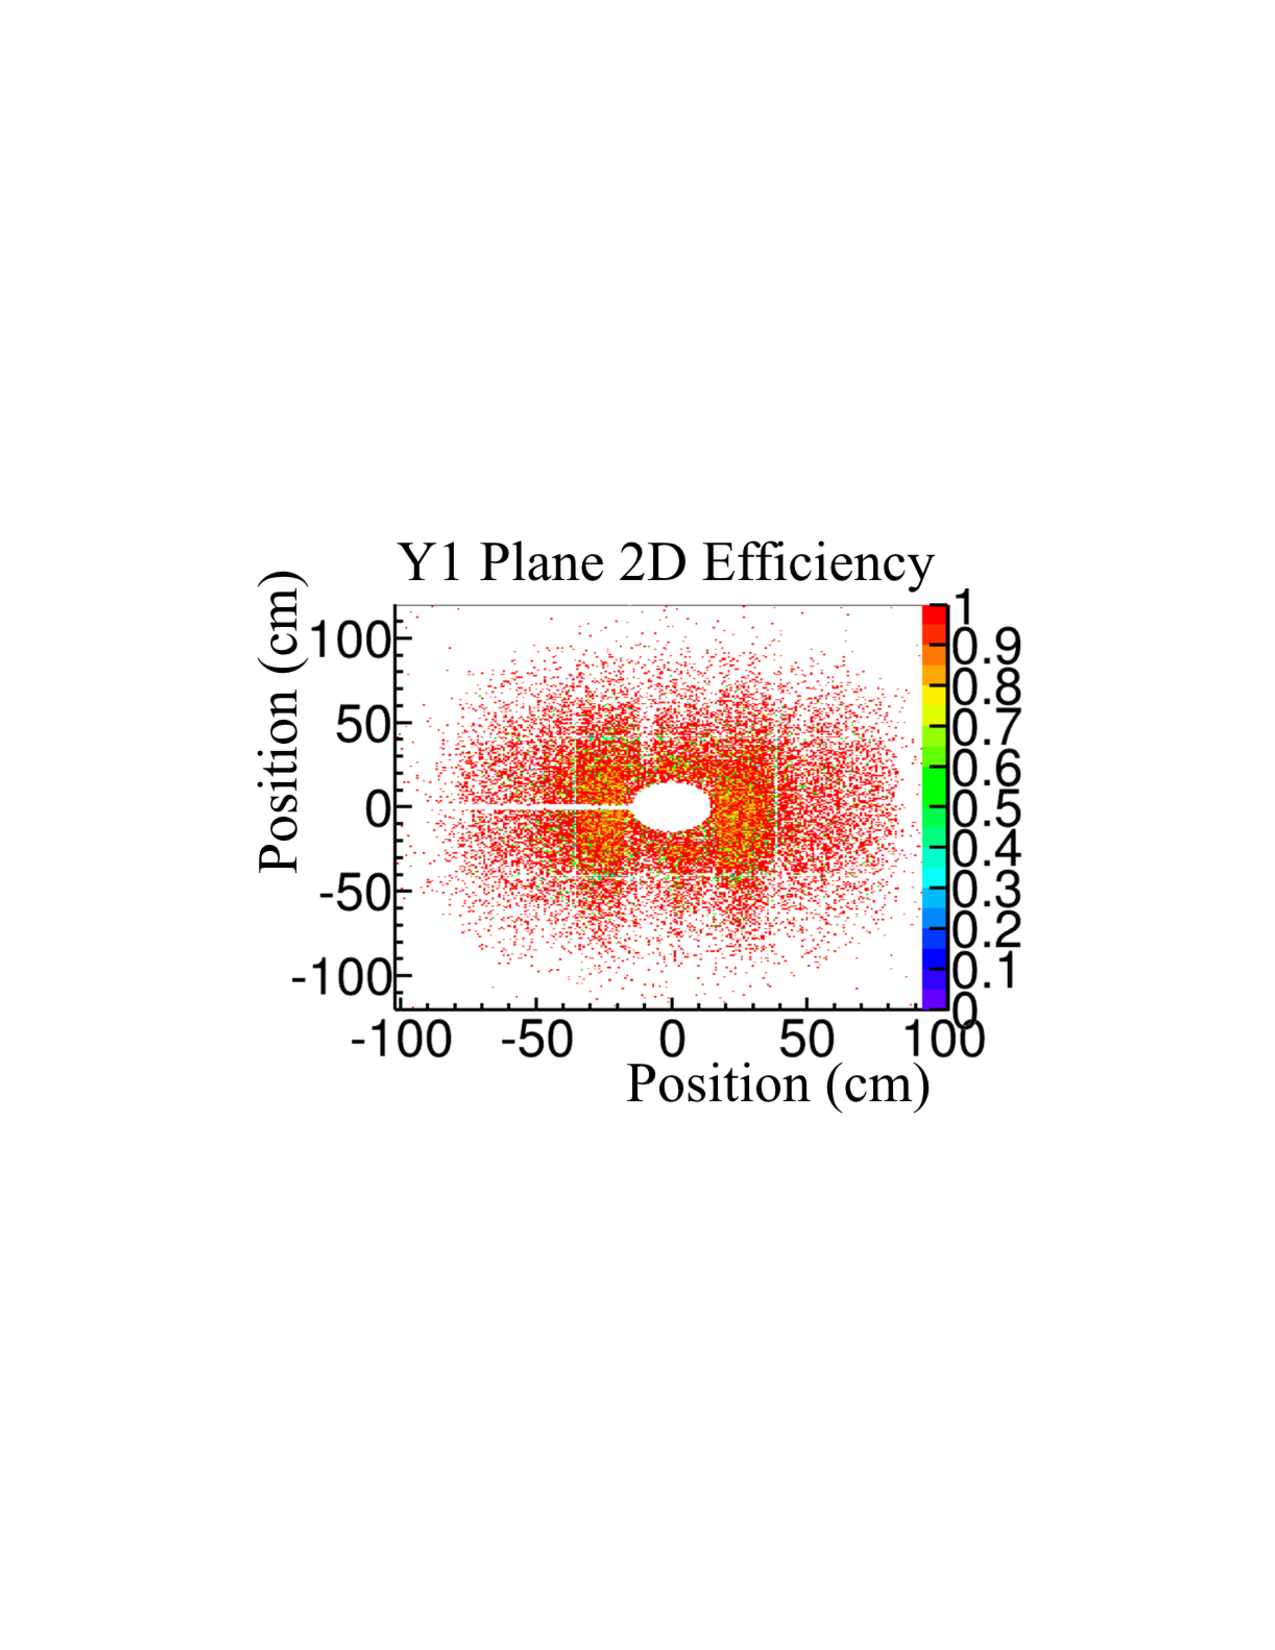
\includegraphics[width=0.6\textwidth, trim=2cm 9cm 2cm 7cm,
    clip]{DC05Yeff}
  \caption{}{Two dimensional efficiency on the DC05Y1 plane.  The center region
    with zero efficiency is a result of the beam killer.}
  \label{fig::DC05Yeff}%
\end{figure}

\begin{figure}[h!t]
  \centering 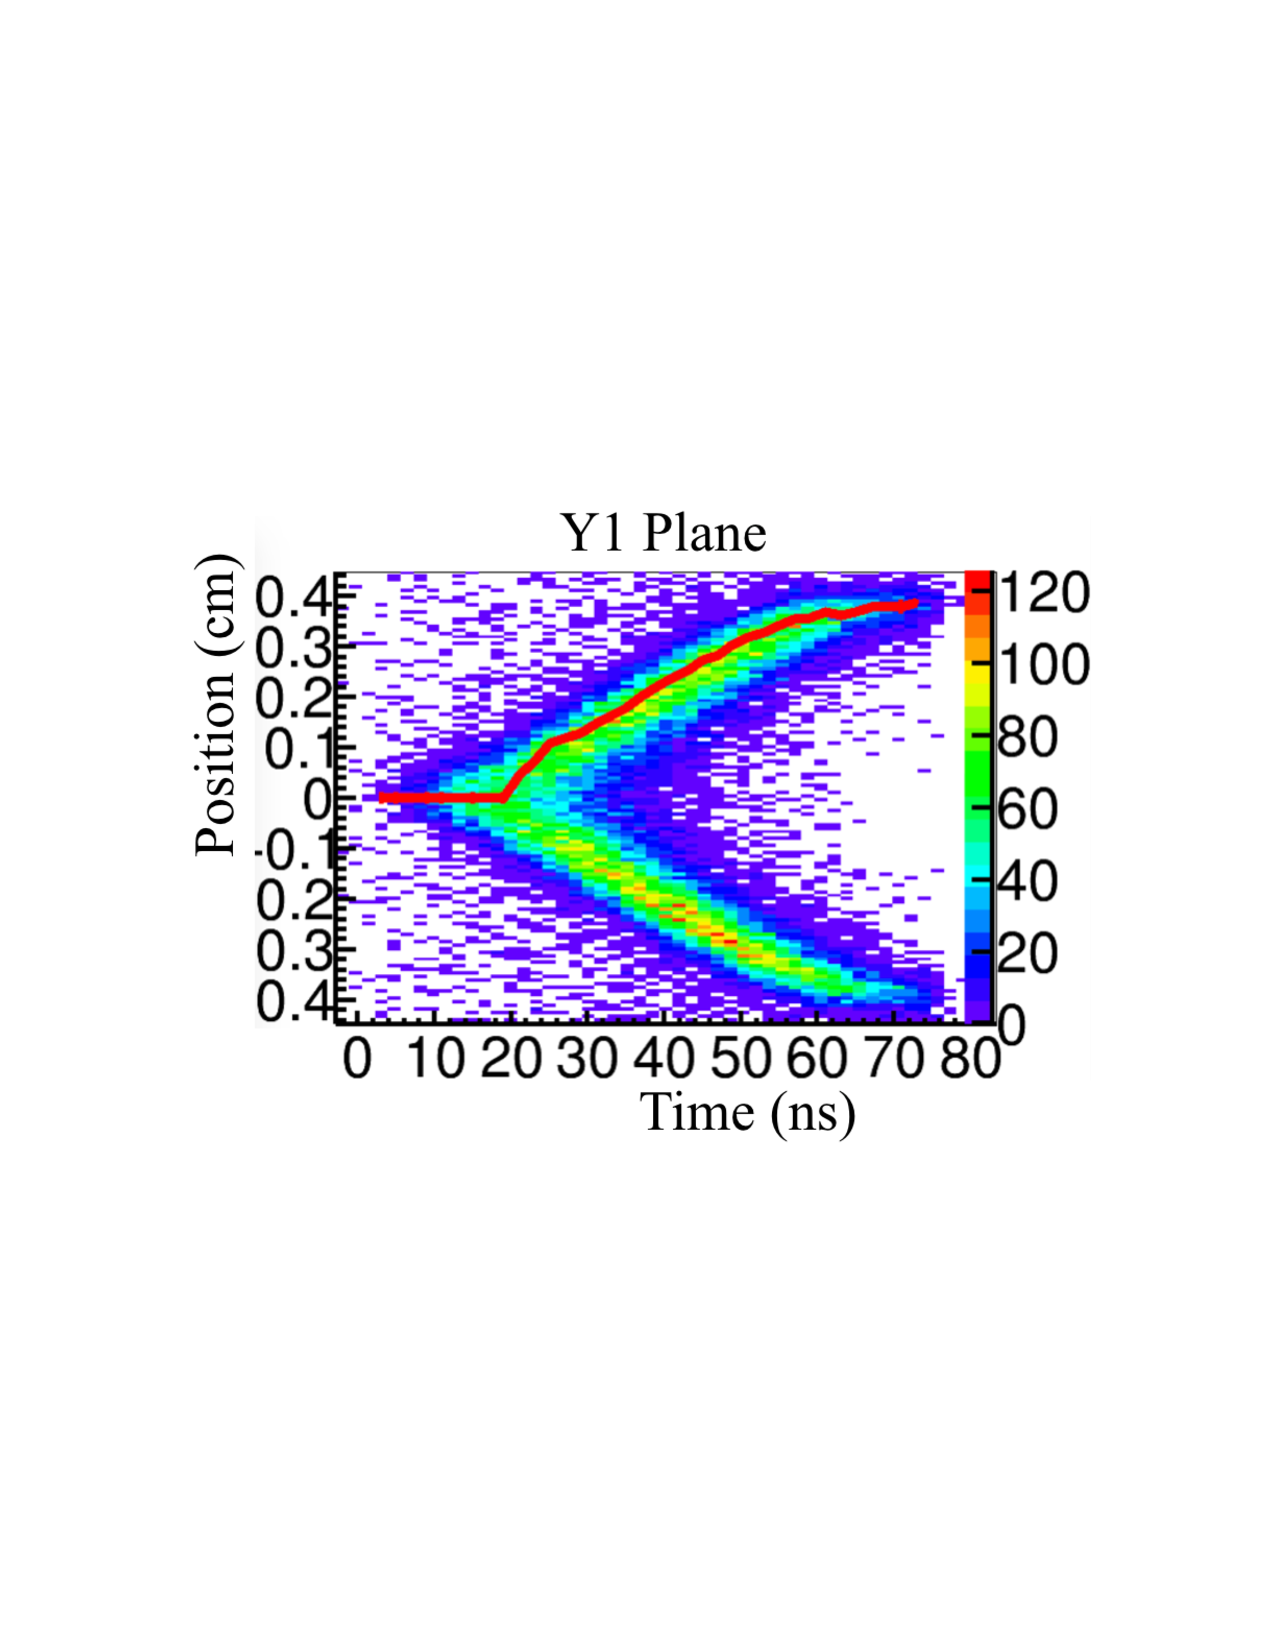
\includegraphics[width=0.6\textwidth, trim=3cm 9cm 3cm 8cm,
    clip]{RT_DC05Y2}
  \caption{}{Time versus position relation, or RT relation, after calibrating.
    The red fit shows the calibration determined.}
  \label{fig:RT_DC05Y2}%
\end{figure}

The double layer residual was used to determine the position resolution.  The
double layer residual is the difference between the expected positions of the
two planes in a view.  The double residual is defined as

\begin{equation}
  \label{equ::doubleRes}
  \Delta \mathrm{u}_{\mathrm{double \; residual}} = (\mathrm{u}_{\mathrm{plane
      \; 1}} - \mathrm{u}_{\mathrm{track}}) - (\mathrm{u}_{\mathrm{plane \; 2}}
  - \mathrm{u}_{\mathrm{track}}) = \mathrm{u}_{\mathrm{plane \; 1}} -
  \mathrm{u}_{\mathrm{plane \; 2}},
\end{equation}
\noindent
where u$_{\mathrm{plane \; 1(2)}}$ is the hit position on plane 1(2) determined
from the detector of interested and u$_{\mathrm{track}}$ is the hit position
determined from reconstruction.  As can be seen in Eq.~\ref{equ::doubleRes}, the
double layer residual is independent of the track resolution and only depends on
the difference between detector hit positions.  As the detector was construction
with a known difference between these two cell hit positions, the double
residual distribution is expected to be a constant value.  Therefore the
variance of the double residual distribution is the addition of the variance of
the two individual planes.  That is

\begin{equation}
\sigma_{\mathrm{double \; residual}}^2 = \sigma_{\mathrm{plane \; 1}}^2 +
\sigma_{\mathrm{plane \; 2}}^2 = 2*\sigma_{\mathrm{plane \; 1}}^2,
\end{equation}

\noindent
where $\sigma_{\mathrm{plane \; 1(2}}$ is the position resolution of plane 1(2).
It is assumed that the position resolution is the same for each plane and
therefore

\begin{equation}
\sigma_{\mathrm{plane \; 1}} = \sigma_{\mathrm{plane \; 2}} =
\frac{\sigma_{\mathrm{double \; residual}}}{\sqrt{2}}
\end{equation}

\noindent
For the 2015 Drell-Yan physics taking the resolution achieved was
approximately 430~$\mu$m. This was determined by fitting the double residual
with a Gaussian to extract the variance and assuming equal variance per plane in
a view as is shown in Fig.~\ref{fig::DC05doubleRes}.

\begin{figure}[h!t]
  \centering 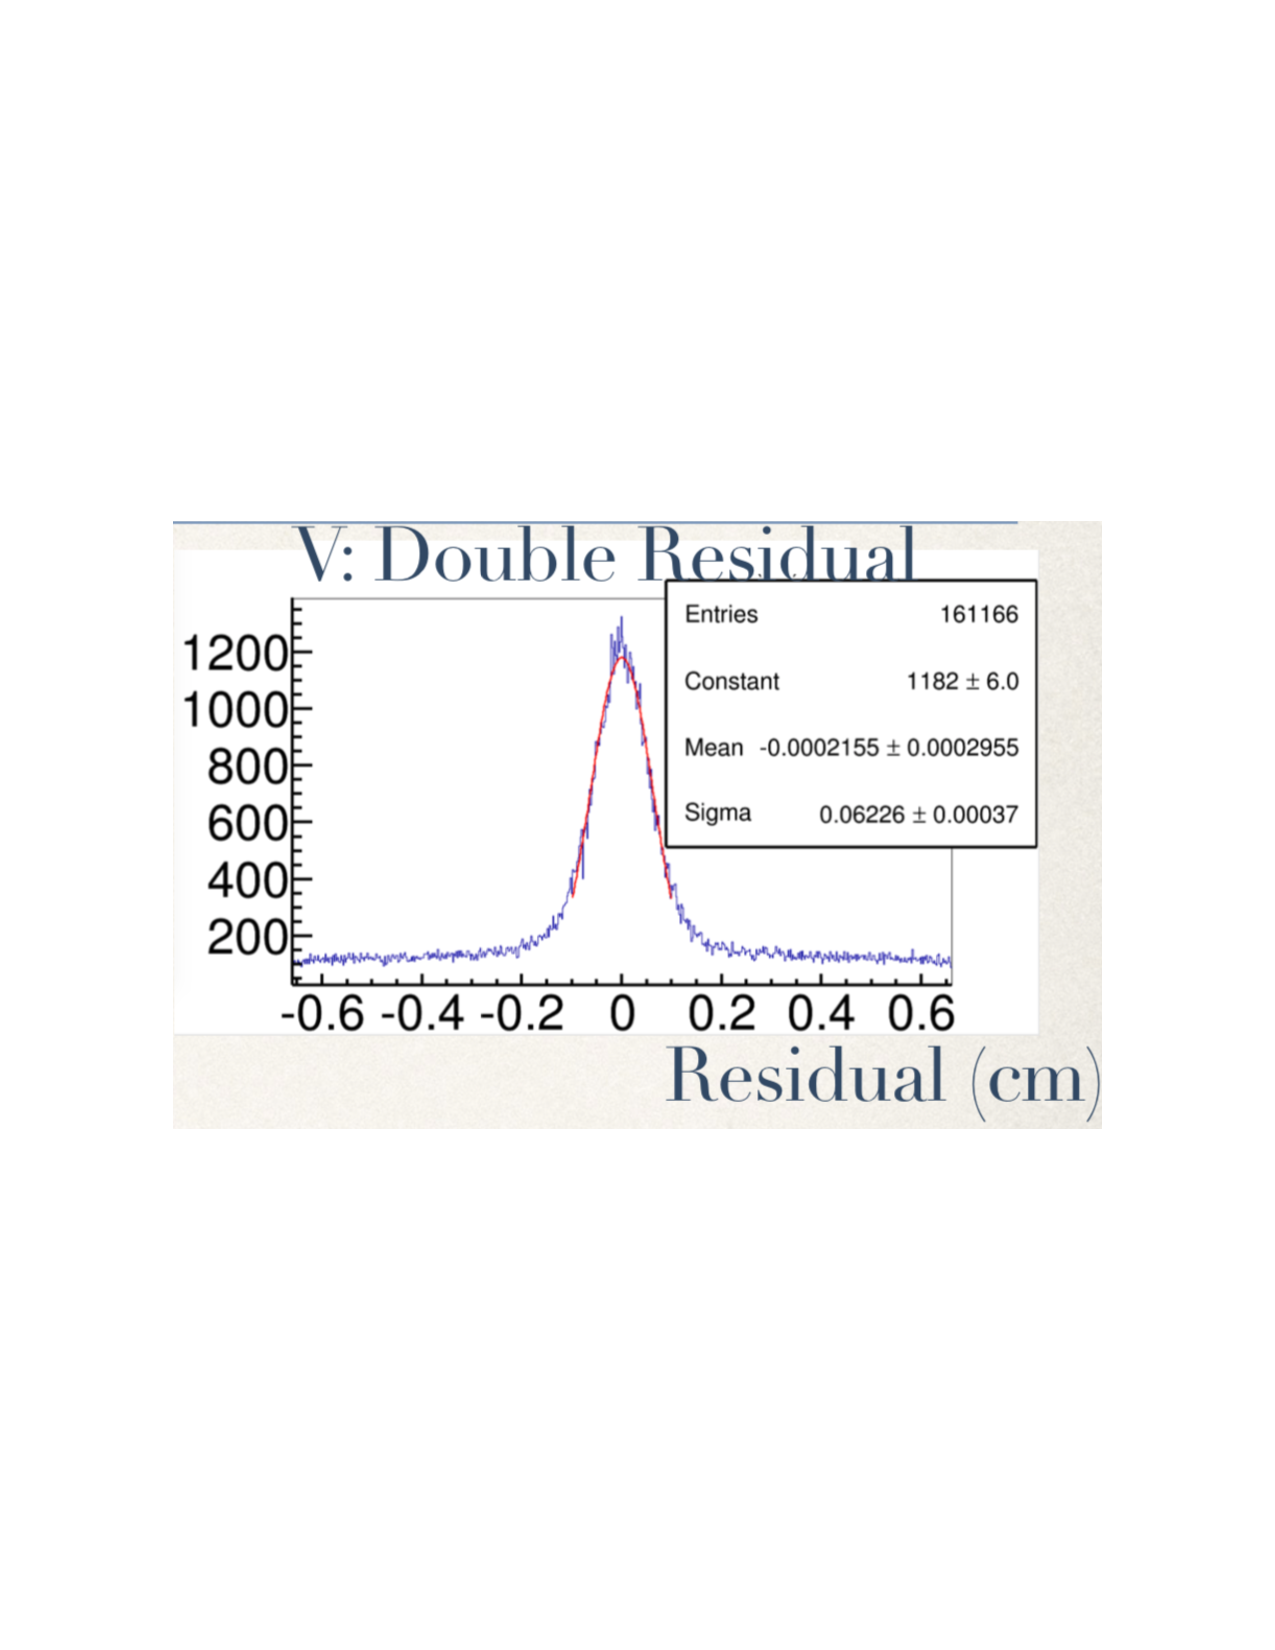
\includegraphics[width=0.6\textwidth, trim=2cm 9cm 2cm 8cm,
    clip]{DC05doubleRes}
  \caption{The double residual distribution for the V plane together with a
    Gaussian fit in red to determine the variance of the distribution}
  \label{fig::DC05doubleRes}
\end{figure}

%\chapter{Spectrometer Alignment} \label{ch::alignment}
\ifpdf
\graphicspath{{Chapters/Alignment/Figs/Raster/}{Chapters/Alignment/Figs/PDF/}{Chapters/Alignment/Figs/}}
\else \graphicspath{{Chapters/Alignment/Figs/Vector/}{Chapters/Alignment/Figs/}}
\fi

The alignment of the spectrometer is important for track reconstruction.
Alignment is a part of pre-processing which ensures all the tracking detectors
are centered relative to each other and therefore enables the track resolution
to be as accurate as possible.  Without accurate alignment, track reconstruction
is not possible and it is therefore not possible to analyze any data.  The
author of this thesis oversaw collection of alignment data and was
responsible for performing the alignment of the COMPASS spectrometer in 2015.

The objective of the alignment procedure is to produce a file called the
detectors.dat.  This file describes the parameters for all detectors at COMPASS
and in particular, gives their orientation in space.  For a tracking detector
plane, there are four parameters the alignment procedure updates: the x central
position, y central position, angle and the pitch.  The pitch refers to a sense
wire distance for wire chambers or central strip separation distance for
detectors with strip readouts.  One or two detectors.dat files was produced for
each data taking period, depending on how many alignment runs were recorded that
period.  The goal of the alignment procedure is to have all four parameters
aligned relative to a global reference frame in the COMPASS lab system.

The alignment procedure works by minimizing the distance between all the
detector plane hit positions and a track position.  The detector hit position is
the location the detector believes a particle passed through the plane and the
track position is the location the reconstruction believes the particle passed
through the detector plane.  The distance between this detector plane hit
position and the track position will from here on be referred to as the residual
distance.  One residual is determined per track per detector associated with the
track.  The task of simultaneously minimizing all the residuals is difficult
because there are over 300 detectors planes described in the detectors.dat.  To
accomplish this minimization, a large amount of quality data is needed and
several specific matrix manipulations are utilized in the minimization
procedure.  This chapters gives an overview of the alignment procedure and
includes some results from 2015.  For a more complete review see
reference~\cite{compassAlignmentNote}.


\section{Alignment Data}

The alignment data is produced from a dedicated low intensity muon beam.  The
intensity in 2015 was approximately 10$^5 \mu^-$/spill.  A muon beam is
desirable for alignment data because the beam muons interact less and therefore
allows the alignment procedure to assume straight tracks in the minimization
problem.  The lower intensity is chosen because this allows for the assumption
that only one track occurs per event and also the low intensity beam ensures a
reduction of detector pile up effects.  Reduction in pile up effects, makes
reconstruction in the central detector areas possible, and therefore the beam
killers on DC00, DC01, DC04 and DC05 can be set to an amplification voltage and
as well all the GEM detectors can have their central high voltages turned up to
an amplification voltage.

A dedicated trigger system is setup during alignment runs to maximize the
illumination of the tracking detectors.  The triggers used are a beam trigger,
veto trigger and a halo trigger.  While this trigger was good for illuminating
the detectors, there were some timing shifts relative to the normal Drell-Yan
trigger in 2015.  For this reason some of the drift chambers used a different
calibration curve shifted in time a few nanoseconds.

Two alignment runs of good quality are recorded either at the beginning, middle
or end of a data taking period.  The first alignment run is with the
spectrometer magnets off and the second is with the spectrometer magnets on.
The spectrometer magnets off run is used as a first iteration for the alignment
procedure to initialize the tracking detector positions.  The final alignment
positions are then determined from the spectrometer magnets on data.  

One physics run was also used to align detectors far from the beam line.
Particularly, the outer region of the straw detectors did not receive enough
statistics from the aligning runs.  Therefore the alignment of the outer straw
regions was performed with normal physics data.  The runs used for alignment
analysis in 2015 are listed in Table~\ref{tab::alignmentRuns}.

In 2015 the alignment runs were performed when the target solenoid was
polarizing the target.  The chicane magnets upstream of the target were
therefore turned off to ensure the beam momentum was traveling along the target
axis.  Normally to achieve the reduced intensity, the T6 target is switch to an
air target.  However in 2015, the T6 target head was not able to switch between
the different target lengths and therefore the maximum 500~mm target head was
always in use.  Therefore to achieve the desired lower intensity, a set of
collimeters upstream of the target reduced the aperture of the beam line till
the correct intensity was achieved.

\begin{table}[h!t]
  \centering
  \begin{tabular}{ |c|c|c|c|c|c| }
    \hline
    \textbf{Period}& \textbf{Sub-period}& \textbf{Magnets off run}&
    \textbf{Magnets on run}& \textbf{Physics run}&
    \textbf{detectors.dat name} \\ \hline
    
    W07& one \& two & 259360& 259361& 259363& detectors.259361.transv.dat
    \\ \hline

    W08& one \& two & 260072& 260073& 260100& detectors.260073.transv.dat
    \\ \hline

    \multirow{2}{2em}{W09}& one& 260625& 260626& 260661&
    detectors.260626.transv.dat \\
    & two& 260625& 260876& 261312&
    detectors.260876.transv.dat \\ \hline

    \multirow{2}{2em}{W10}& one& 261512& 261513& 261602&
    detectors.261513.transv.dat \\
    & two& 261512& 261513& 261974&
    detectors.261970.transv.dat \\ \hline

    W11& one \& two & 262423& 262425& 262612& detectors.262370.transv.dat
    \\ \hline

    W12& one \& two & 263139& 263140& 263175& detectors.263140.transv.dat
    \\ \hline

    W13& one \& two & 263636& 263637& 263851& detectors.263637.transv.dat
    \\ \hline

    W14& one \& two & none& 264428& 264429& detectors.264163.transv.dat
    \\ \hline

    W15& one \& two & 264614& 264722& 264736& detectors.264619.transv.dat
    \\ \hline
    
  \end{tabular}
  \caption{COMPASS 2015 alignment data runs}
  \label{tab::alignmentRuns}
\end{table}


\section{Procedure}

The starting point for alignment is a detectors.dat file with the tracking
detector positions determined from a survey.  The surveys are performed with the
spectrometer magnets off and the precision from a survey is around 1~mm.  Almost
all of the detectors at COMPASS have a position resolution better than the
survey precision however.  Furthermore, several detectors near SM1 can shift in
position due to the fringe field and therefore need a position determination
with the spectrometer magnets on.  For these reasons the alignment procedure is
needed to improve on the survey precision and achieve the best possible track
resolutions.

Between periods the starting detectors.dat file was the final detectors.dat from
the previous week.  Only for the first period were the survey positions used as
a starting position.  However, as long as the detector was not intentionally
moved, it is expected that the shifts in detector position only change due to
temperature effects and therefore do not change much.

\subsubsection{Alignment Parameters}

To best describe each detector relative to every other detector there are two
reference systems of interest.

The first reference system is the COMPASS main reference system labeled
\textit{Oxyz}.  This reference system can also be referred to as the COMPASS lab
system, where the z-axis is along the beam momentum direction, the y-axis points
vertically and the x-axis is such that the coordinate system is right handed.
The origin of this reference system is at the center of the target from the
original COMPASS setup.

The second reference system is the local reference system, which is labeled as
\textit{O'uvz}.  This reference system is different for each detector and has
its origin at the center of each detector center.  The z-axis coincides with the
z-axis in the COMPASS main reference system while the u-axis is in the direction
along the measured coordinate of the detector, and the v-axis is perpendicular to
the direction of the measured coordinate of this detector.  As an example, a drift
chamber with vertical wires measures a coordinate along the horizontal direction
and therefore it's u-axis is in the horizontal direction and it's v-axis is in
the vertical direction.  A drift chamber with horizontal wires, however,
measures a coordinate along the vertical direction and therefore it's u-axis is
in the vertical direction and it's v-axis is in the horizontal direction.

The alignment parameters are defined in \textit{O'uvz}.  The alignment procedure
updates the starting detectors.dat file by the shifts

\begin{align}
  \delta \mathrm{u} & \mathrm{: \; shift \; in \; u \; direction,}  \\
  \delta \theta & \mathrm{: \; shift \; in \; rotation \; angle,}  \\
  \delta \mathrm{z} & \mathrm{: \; shift \; in \; z \; direction,}  \\
  \delta \mathrm{p} & \mathrm{: \; shift \; in \; pitch.} 
\end{align}
\noindent
The shift in z direction has never converged however.  As a result the
z-coordinate from the survey is used as the final z position and the shift in
pitch is used as an effective shift in the z direction.

\subsubsection{Residual Function}

The goal of the alignment procedure is to minimize the sum of all the residuals
from each track and each detector associated with the track.  Due to the fact
that the alignment tracks are assumed to be straight, each track can be defined
by four parameters.  The track parameters, {\atrack}, are

\begin{enumerate}[label=\roman*:]
\item (x$^0$, y$^0$) the x and y coordinates at the main reference origin
\item (t$_{\mathrm{x}}^0$, t$_{\mathrm{y}}^0$) the tangents of the track
  momentum in the x and y directions at the origin of the main reference system
\end{enumerate}
\noindent
where the track parameters are defined for each track.  The alignment parameters
, {\adet}, on the other hand are defined for each detector and are the same for
all tracks.  The alignment procedure minimizes the $\chi^2$ function

\begin{equation}
  \chi^2 =
  \sum_{i=1}^{i=n_{\mathrm{tracks}}}\sum_{j=1}^{j=n_{\mathrm{detectors}}}
  \frac{\mathrm{F}^2_{i,j}(\alpha_{\mathrm{T}, i}, \alpha_{\mathrm{D},
      j})}{\sigma_j^2},
  \label{equ::chi_align}%
\end{equation}
\noindent
where $\sigma^2_j$ is the position resolution of detector j, F$_{i,j}$ is the
residual distance of each detector j for each track i it is associated with.

The residual distance, F, depends on the track parameters and the detector
parameters.  For magnets off data the tracks are not bent at all and are
therefore straight tracks through out the whole spectrometer.  The x and y coordinates at position z are

\begin{align}
  \label{equ::trackPosOff}
  \mathrm{x} &= \mathrm{x}^0 +
  \mathrm{t}_{\mathrm{x}}^0(\mathrm{z}-\mathrm{z}^0), \\
  \mathrm{y} &=
  \mathrm{y}^0 + \mathrm{t}_{\mathrm{y}}^0(\mathrm{z}-\mathrm{z}^0),
\end{align}
\noindent
where z$^0$ refers to the position at the origin in \textit{Oxyz}.
Rotating these track positions from the main references system, \textit{Oxyz},
to the detector reference system, \textit{O'uvz}, the residual distance is

\begin{equation}
\mathrm{F} = \cos(\theta)[\mathrm{x}^0 +
  \mathrm{t}_{\mathrm{x}}^0(\mathrm{z}-\mathrm{z}^0)] +
\sin(\theta)[\mathrm{y}^0 + \mathrm{t}_{\mathrm{y}}^0(\mathrm{z}-\mathrm{z}^0)]
- \mathrm{u},
\end{equation}
\noindent
where u is the measured hit position from the detector at position z.  To show
the dependence on the alignment parameters

\begin{dmath} \label{equ::Falign}
  \mathrm{F}(\alpha_{\mathrm{T}}, \alpha_{\mathrm{D}}+\delta\alpha_{\mathrm{D}})
  = (1+\delta \mathrm{p})
  \Big \{ \cos(\theta + \delta \theta)
       [\mathrm{x}^0 + \mathrm{t}^0_{\mathrm{x}}(\mathrm{z}-\mathrm{z}^0)] +
       \sin(\theta + \delta \theta)[\mathrm{y}^0 + \mathrm{t}^0_{\mathrm{y}}
         (\mathrm{z}-\mathrm{z}^0)] \Big \} -
       (\mathrm{u} + \delta \mathrm{u}).
\end{dmath}
\noindent
In Eq.~\ref{equ::Falign}, the change in pitch would intuitively affect the u
position, however the change in pitch was moved to the track coordinates to make
derivatives of F independent of u.  This has no effect on the minimization of F.

In the case of magnets on data, the track positions need to have further
modifications from Eq.~\ref{equ::Falign}.  The magnetic field will bend the
tracks so the track positions determined in Eq.~\ref{equ::trackPosOff} need to
have further corrections.  The track positions with SM1 and SM2 on are
\begin{align}
  \label{equ::trackPosOn}
  \mathrm{x} &= \mathrm{x}^0 + \delta\mathrm{x} +
  (\mathrm{t}_{\mathrm{x}}^0 + \delta \mathrm{t}_{\mathrm{x}})
  (\mathrm{z}-\mathrm{z}^0), \\
  \mathrm{y} &= \mathrm{y}^0 + \delta\mathrm{y} +
  (\mathrm{t}_{\mathrm{y}}^0 + \delta \mathrm{t}_{\mathrm{y}})
  (\mathrm{z}-\mathrm{z}^0),
\end{align}
\noindent
where the $\delta_{\mathrm{x}}$, $\delta \mathrm{t}_{\mathrm{x}}$,
$\delta_{\mathrm{y}}$ and $\delta \mathrm{t}_{\mathrm{y}}$ changes are
determined from CORAL during the reconstruction process.  Even though the
spectrometer magnets have nominally vertical magnetic fields, there are still
fringe fields which are not vertical.  It is for this reason that CORAL also
calculates an updated track position in the y-coordinate.

The residual dependence on the alignment parameters defined for magnetic fields
on is then
\begin{dmath}
  \mathrm{F}(\alpha_{\mathrm{T}},
  \alpha_{\mathrm{D}}+\delta\alpha_{\mathrm{D}}) = 
  (1+\delta \mathrm{p})\Big \{
\cos(\theta + \delta \theta)[\mathrm{x}^0 + \delta\mathrm{x} +
  (\mathrm{t}^0_{\mathrm{x}}+\delta \mathrm{t}_{\mathrm{x}})
  (\mathrm{z}-\mathrm{z}^0)] +
\sin(\theta + \delta\theta)[\mathrm{y}^0 + \delta\mathrm{y} +
  (\mathrm{t}^0_{\mathrm{y}}+\delta \mathrm{t}_{\mathrm{y}})
  (\mathrm{z}-\mathrm{z}^0)]
\Big \}
- (\mathrm{u} + \delta \mathrm{u}).
\end{dmath}

\subsubsection{$\chi^2$ Minimization}
The $\chi^2$ function, Eq.~\ref{equ::chi_align}, is analytically minimized.
That is, the derivatives of Eq.~\ref{equ::chi_align} with respect to all the
track and alignment parameters are set to zero and these alignment parameters
are solved for.  This can be written

\begin{equation}
  \label{equ::chi2analytic}
  \frac{1}{2}\frac{\partial \chi ^2}{\partial \alpha_k} =
  \sum_{i}^{n_{\mathrm{tracks}}} \sum_j ^{n_{\mathrm{detectors}}}
  \frac{1}{\sigma_j^2}\frac{\partial \mathrm{F}_{i,j}}{\partial \alpha_k}
  \mathrm{F}_{i,j} = 0.
\end{equation}

\noindent
To perform this calculation the residual function is Taylor expanded in the
track and alignment parameters as
\begin{equation}
\mathrm{F} = \mathrm{F}^0 + \sum_k \frac{\partial \mathrm{F}}{\partial
  \alpha_k}\alpha_k.
\end{equation}

\noindent
Using this approximation for F, Eq.~\ref{equ::chi2analytic} can be written as a
matrix equation where the dimensions of the matrix are
(4n$_{\mathrm{detector}}$+4n$_{\mathrm{tracks}})\times$
(4n$_{\mathrm{detector}}$ +4n$_{\mathrm{tracks}})$.  This matrix form is written
as

\begin{dmath}
  \begin{bmatrix}
    \sum_i^{n_{\mathrm{tracks}}} \sum_j^{n_{\mathrm{detectors}}}
      \frac{1}{\sigma^2_j} \frac{\partial \mathrm{F}_{i,j}}{\partial
        \alpha_{\mathrm{D_1}}}\frac{\partial \mathrm{F}_{i,j}}{\partial
        \alpha_{\mathrm{D_1}}}
      & \dots &
      \sum_j^{n_{\mathrm{detectors}}}
      \frac{1}{\sigma^2_j}\frac{\partial \mathrm{F}_{i,j}}{\partial
        \alpha_{\mathrm{D_1}}}\frac{\partial \mathrm{F}_{i,j}}{\partial
        \alpha_{\mathrm{T_{4\mathrm{n}_{\mathrm{tracks}}}}}} \\
      \vdots & \ddots & \vdots \\
      \sum_j^{n_{\mathrm{detectors}}}
      \frac{1}{\sigma^2_j}\frac{\partial \mathrm{F}_{i,j}}{\partial
        \alpha_{\mathrm{T_{4\mathrm{n}_{\mathrm{tracks}}}}}}\frac{\partial
        \mathrm{F}_{i,j}}{\partial \alpha_{\mathrm{D_1}}} & \dots &
      \sum_j^{n_{\mathrm{detectors}}} \frac{1}{\sigma^2_j}\frac{\partial
        \mathrm{F}_{i,j}}{\partial
        \alpha_{\mathrm{T_{4\mathrm{n}_{\mathrm{tracks}}}}}}\frac{\partial
        \mathrm{F}_{i,j}}{\partial
        \alpha_{\mathrm{T_{4\mathrm{n}_{\mathrm{tracks}}}}}}
  \end{bmatrix}
  \begin{bmatrix}
    \alpha_{\mathrm{D_1}} \\
    \vdots \\
    \alpha_{\mathrm{T_{4\mathrm{n}_{\mathrm{tracks}}}}}
  \end{bmatrix}
  = -
  \begin{bmatrix}
    \sum_i^{n_{\mathrm{tracks}}} \sum_j^{n_{\mathrm{detectors}}}
      \frac{1}{\sigma^2_j}\frac{\partial \mathrm{F}_{i,j}}{\partial
        \alpha_{\mathrm{D_1}}} \mathrm{F}_{i,j}^0 \\
      \vdots \\
      \sum_j^{n_{\mathrm{detectors}}}
    \frac{1}{\sigma^2_j}\frac{\partial \mathrm{F}_{i,j}}{\partial
      \alpha_{\mathrm{T_{4\mathrm{n}_{\mathrm{tracks}}}}}} \mathrm{F}_{i,j}^0
  \end{bmatrix}.
  \label{equ::aliMatrix}
\end{dmath}    

\noindent
To solve Eq.~\ref{equ::aliMatrix}, the matrix on the left side must be inverted.
A normal alignment run however, results in over 200,000 tracks meaning this
matrix is huge and infeasible to invert.  Fortunately many of the entries in the
matrix are zero which allows that this matrix inversion can be reduced to
the inversion of several smaller matrices.

To perform the matrix inversion, note that Eq.~\ref{equ::aliMatrix} can be
written

\begin{equation}
  \label{equ::matrixToInvert}
  \begin{bmatrix}
    \sum_{i} \mathrm{C}_i & \vline \; \vline \; & \dots &
    \mathrm{G}_i & \dots \\
    \hline \hline
    \vdots & \vline \; \vline & \ddots & 0 & 0 \\
    \mathrm{G}^{\mathrm{T}} & \vline \; \vline & 0 \; & \Gamma_i & 0 \\
    \vdots & \vline \; \vline & 0 & 0 & \ddots
  \end{bmatrix}
  \begin{bmatrix}
    \alpha_{\alpha} \\ \hline \hline \vdots \\ \alpha_{\mathrm{T}_i}
    \\ \vdots
  \end{bmatrix}
  =
  \begin{bmatrix}
    \sum_i b_i \\ \hline \hline \vdots \\ \beta_i \\ \vdots
  \end{bmatrix},
\end{equation}

\noindent
where $\sum_i$C$_i$ and $\sum_i$b$_i$ include only derivatives of F$_{i,j}$ with
respect to alignment parameters, $\Gamma_i$ and $\beta_i$ include only
derivatives of F$_{i,j}$ with respect to track parameters and G$_i$ includes
derivatives of F$_{i,j}$ with respect to both alignment and track parameters.
Then reference~\cite{matrix_inv} shows that Eq.~\ref{equ::matrixToInvert} can be
inverted to give the alignment parameters as

\begin{equation}
\alpha_{\alpha} = \mathrm{C'}^{-1}\mathrm{b}',
\end{equation}
\noindent
where
\begin{equation}
\mathrm{C}' = \sum_i \mathrm{C}_i - \sum_i \mathrm{G}_i \Gamma_i^{-1}
\mathrm{G}_i^{\mathrm{T}},
\end{equation}
\noindent
and
\begin{equation}
\mathrm{b}' = \sum_i \mathrm{b}_i - \sum_i \mathrm{G}_i \Gamma_i^{-1}\beta_i.
\end{equation}


\section{Results}

The spectrometer alignment is performed in iterative steps.  In each iteration
of the alignment procedure, the matrix inversion, Eq~\ref{equ::matrixToInvert},
is performed and the alignment parameters are updated.  All alignment tracks
reconstructed in the first alignment iterations are based off of two pivot
detectors.  That is straight track parameters were determined from these two
pivot detectors and all detectors were aligned relative to these pivot
detectors.  In 2015 the pivot detectors were GM05 in LAS and GM08 in SAS.  After
each iteration the detector parameters are updated to reduce the overall
$\chi^2$ value.  Each new iteration is performed using the same data set and the
alignment parameters are better described with each iteration.

The procedure used in 2015 was as follows:
\begin{enumerate}
\item Align with magnets off data.  In this stage all the spectrometer detectors
  except the outer regions of the straw detectors are aligned.  This includes
  all the detectors downstream of the polarized target but does not include the
  beam telescope detectors.  Magnets off data is used as a first iteration and
  therefore only alignment in the u-coordinate is performed.
\item Align the same spectrometer detectors with magnets on data.  In these
  iterations the detectors are aligned for u-coordinate, angle and pitch.
\item Align the beam telescope detectors with magnets on data.  In these
  iterations the previous detectors are all used as pivots.  The beam telescope
  is therefore aligned relative to the spectrometer detectors.
\item Finally the outer region of the straws are aligned with physics data.  For
  this alignment, the spectrometer detectors are again used as the pivot.
\end{enumerate}

The quality of the alignment was monitored after each iteration and checked that
the procedure was converging.  In practice four iterations of each of the
previous steps were found to be sufficient for convergence.  To ensure the
alignment data was from quality tracks, only tracks with momentum reconstructed
and having reduced $\chi^2$ less than 30 were considered.

As all detectors but the pixal detector planes measure a coordinate in one
direction only, the detector positions are only updated in their measured
direction.  This can lead to detectors being well miss-aligned in the direction
orthogonal to their measured coordinate however.  To account for this, detector
planes were updated to match the u-position from a detector plane measuring a
different coordinate in the same detector station.  For example DC04X planes had
their y-coordinate determined from the DC04Y planes and DC04Y planes had their
x-coordinate determined from DC04X planes.

After each alignment iteration the quality of the alignment is accessed for each
individual detectors and for the spectrometer as a whole.  The quality
distributions to check after each iteration are described in the following list.

\begin{enumerate}[label=\roman*)]
\item The residual distribution, $\Delta$u, of each detector.  That is a
  distribution of
  \begin{equation}
    \Delta \mathrm{u} =
    \mathrm{u}_{\mathrm{track}} - \mathrm{u}_{\mathrm{detector}},
  \end{equation}
  where this distribution indicates if the detector is shifted along the
  direction of its measured coordinate.  This distribution is expected to be a
  Gaussian with a zero mean and an RMS value comparable to the position
  resolution of the detector.  Any deviation from a zero mean indicates the
  detector is shifted and a large RMS value indicates the detector is not
  performing as expected.  It the detector is not performing as expected the
  most obvious reason is the calibrations used for that detector are not
  accurate.  Fig.~\ref{fig::PositionResidual} shows an example of this
  distribution to monitor.
  \begin{figure}[h!t]
  \centering 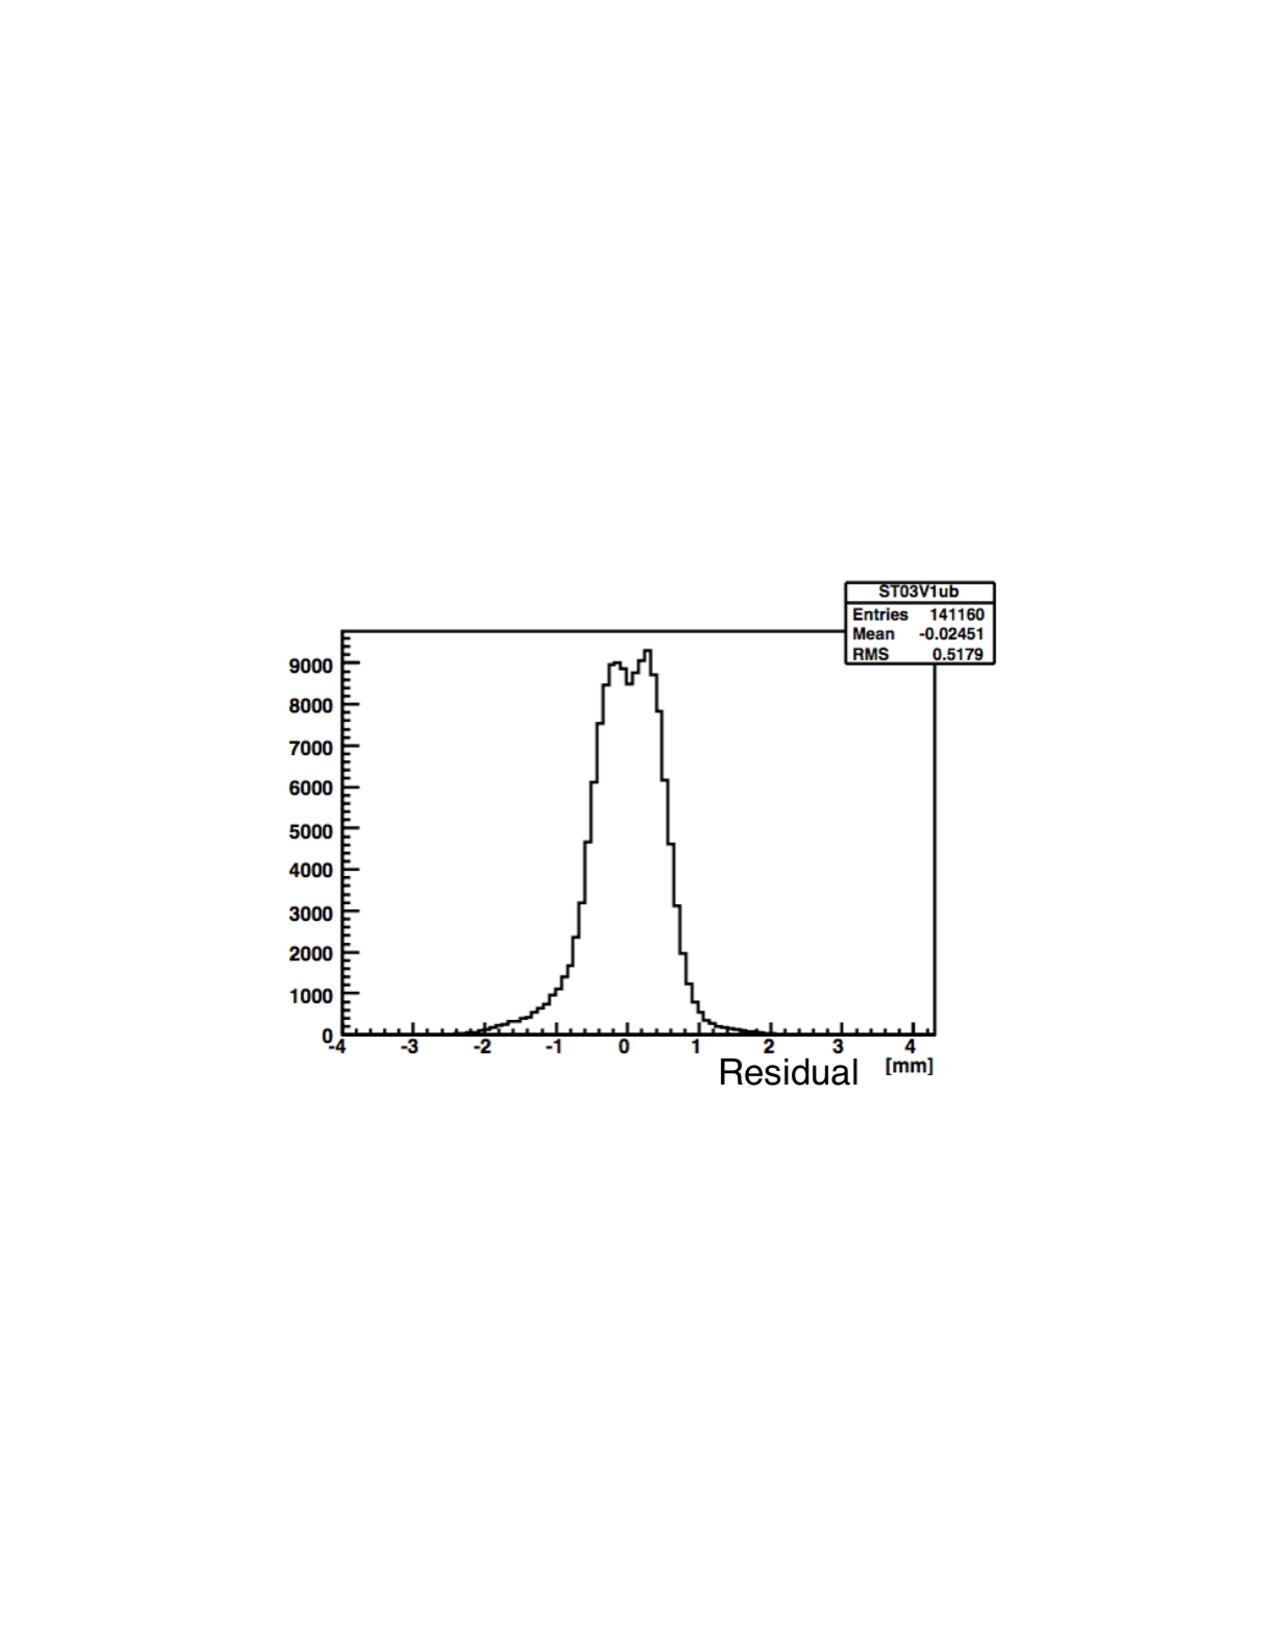
\includegraphics[width=0.5\textwidth, trim=4.5cm 9.5cm 4.5cm 9cm,
    clip]{PositionResidual}
  \caption{The residual distribution for a straw detector plane}
  \label{fig::PositionResidual}
  
\end{figure}
\item The change in the residual as a function of the detector's v-coordinate.
  In a wire detector for example, this is the change in the residual as a
  function of the distance along the wire.  This distribution,
  Fig.~\ref{fig::AngleResidual}, is expected to be uniformly zero.  A slope in
  this distribution indicates that the detector's angle is miss-aligned.
  \begin{figure}[h!t]
    \centering 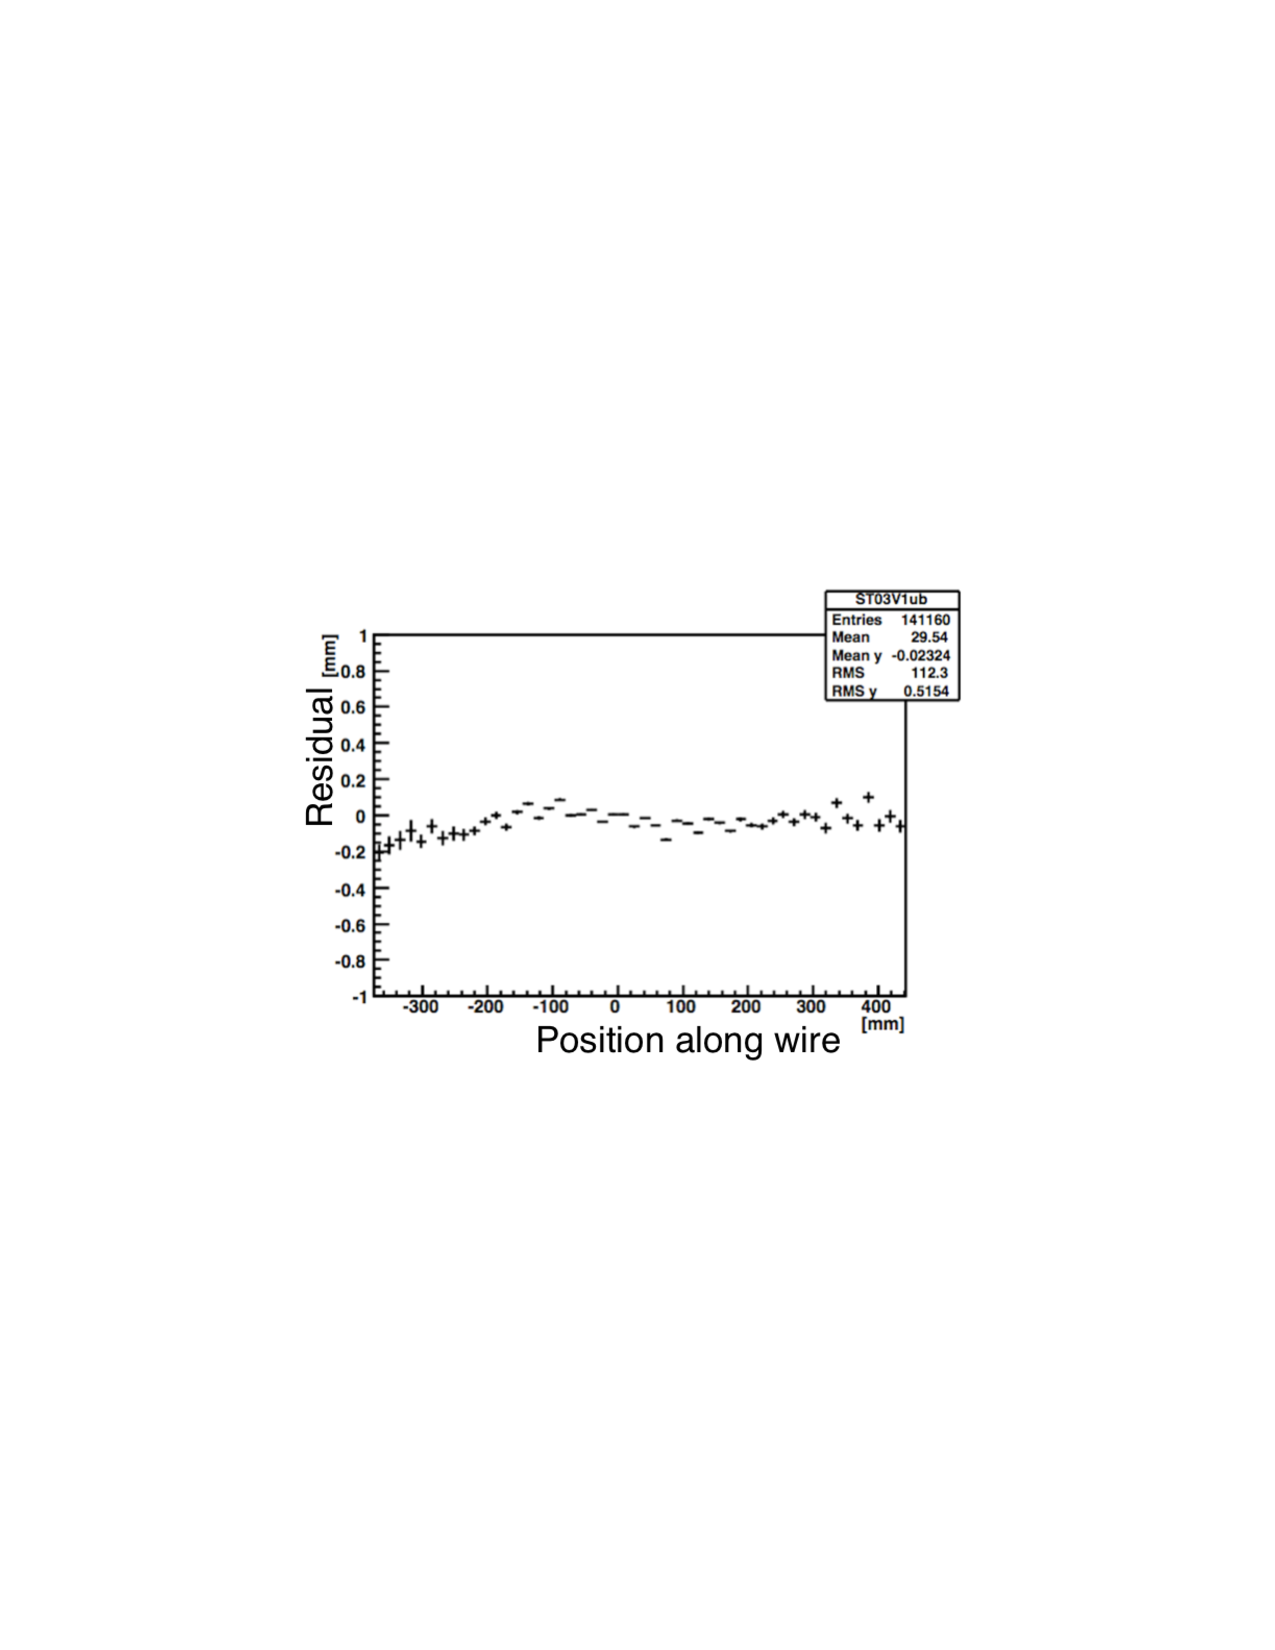
\includegraphics[width=0.5\textwidth, trim=4.5cm 9.5cm 4.5cm 9cm,
      clip]{AngleResidual}
    \caption{The residual as a function of the detector v-coordinate for a straw
      detector}
    \label{fig::AngleResidual}
  \end{figure}
  
\item The change in the residual as a function of the detector's u-coordinate.
  For a wire detector, this is the change in the residual as a function of the
  distance perpendicular to the wire.  This distribution,
  Fig.~\ref{fig::PitchResidual}, is also expected to be uniformly zero.  A slope
  in this distribution indicates that the detector is miss-aligned in it's
  z-coordinate or that its pitch is not described well.  Due to the fact that
  the alignment data is with straight tracks, the alignment in the z-coordinate
  has never been able to converge.  For this reason the pitch of the sensors on
  the detector is changed to account for this effective shift in z-position.
  The sensor pitch however, is never expected to be larger than the true
  detector pitch distance.  If the detector pitch is determined to be too large
  after the alignment, this indicates a problem.
  \begin{figure}[h!t]
    \centering 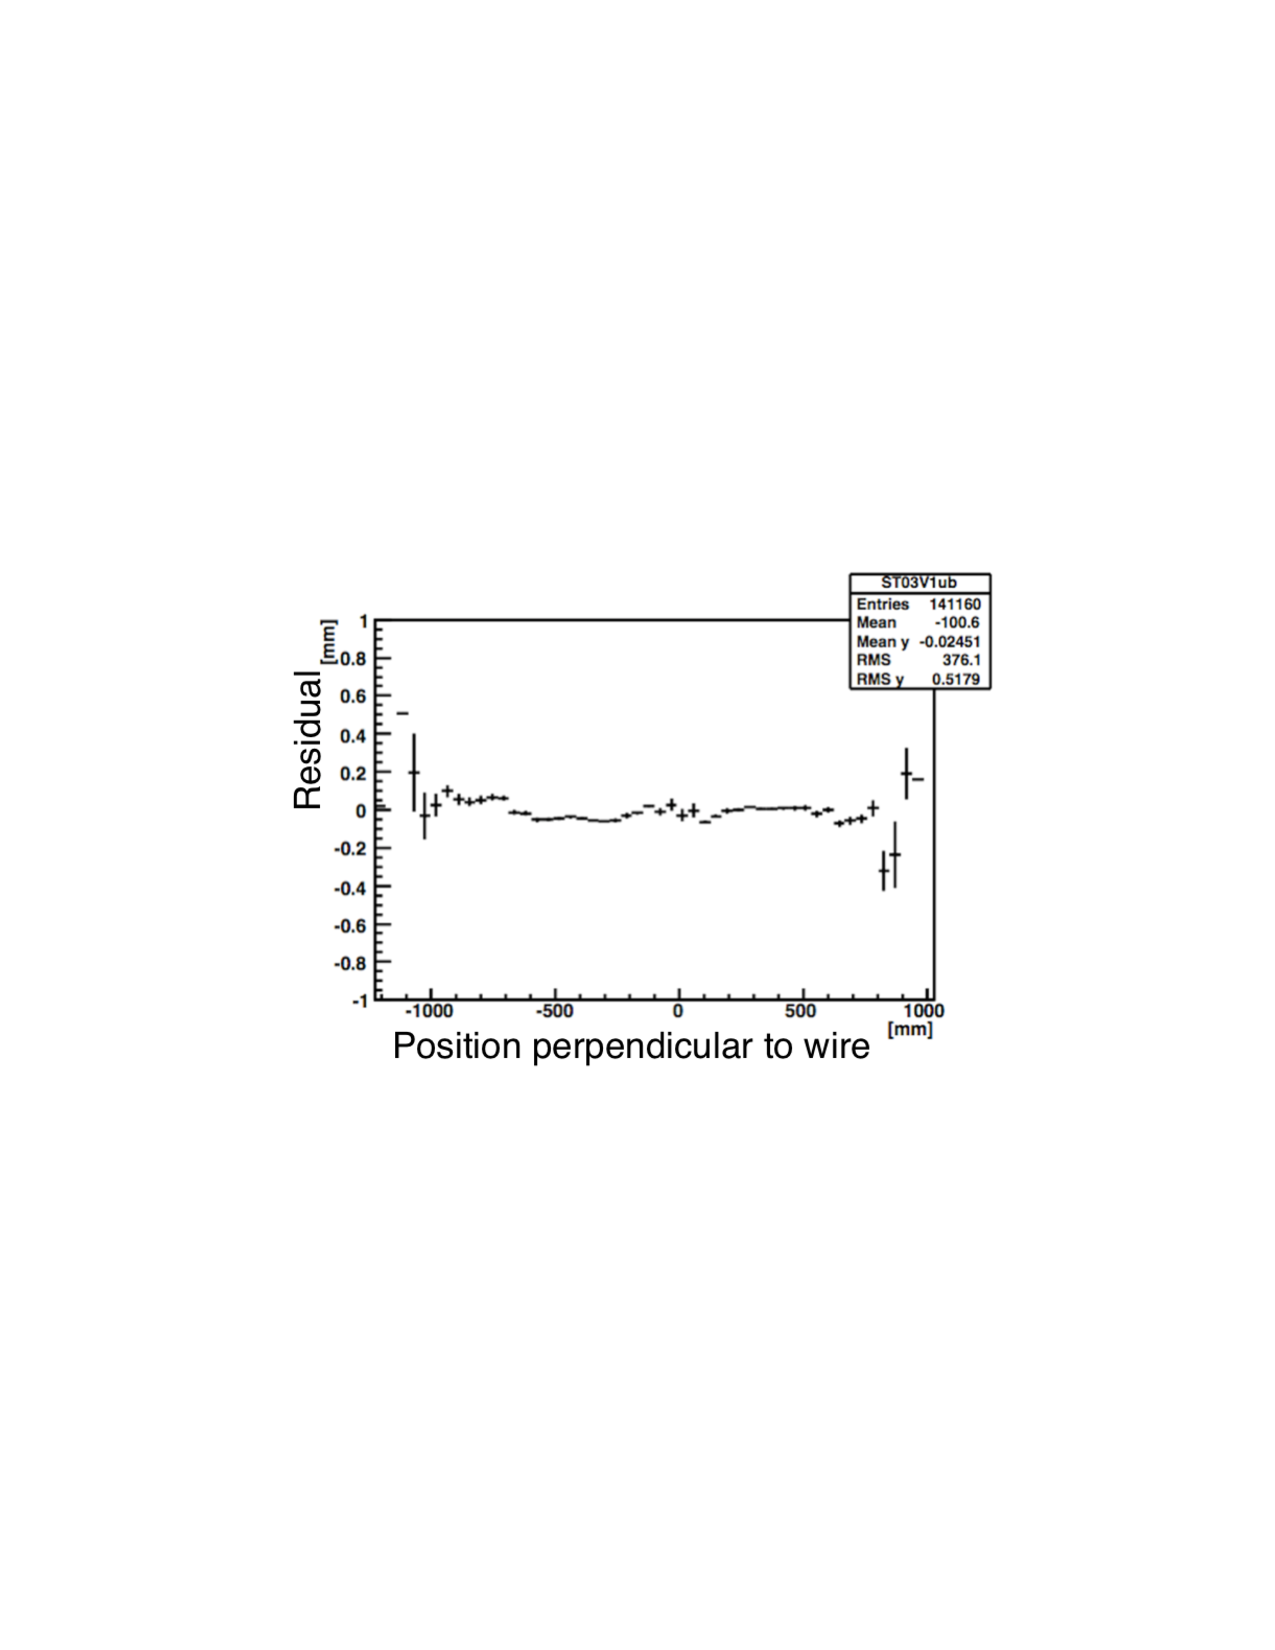
\includegraphics[width=0.5\textwidth, trim=4.5cm 9.5cm 4.5cm 9cm,
      clip]{PitchResidual}
    \caption{The residual as a function of the detector u-coordinate for a straw
      detector}
    \label{fig::PitchResidual}
  \end{figure}

\item The reduced $\chi^2$, Fig.~\ref{fig::trackChi2ndf}, distribution of the
  reconstructed tracks.  With better alignment the track reduced $\chi^2$
  distribution will approach a theoretical distribution of a reduced $\chi^2$
  distribution.
  \begin{figure}[h!t]
    \centering 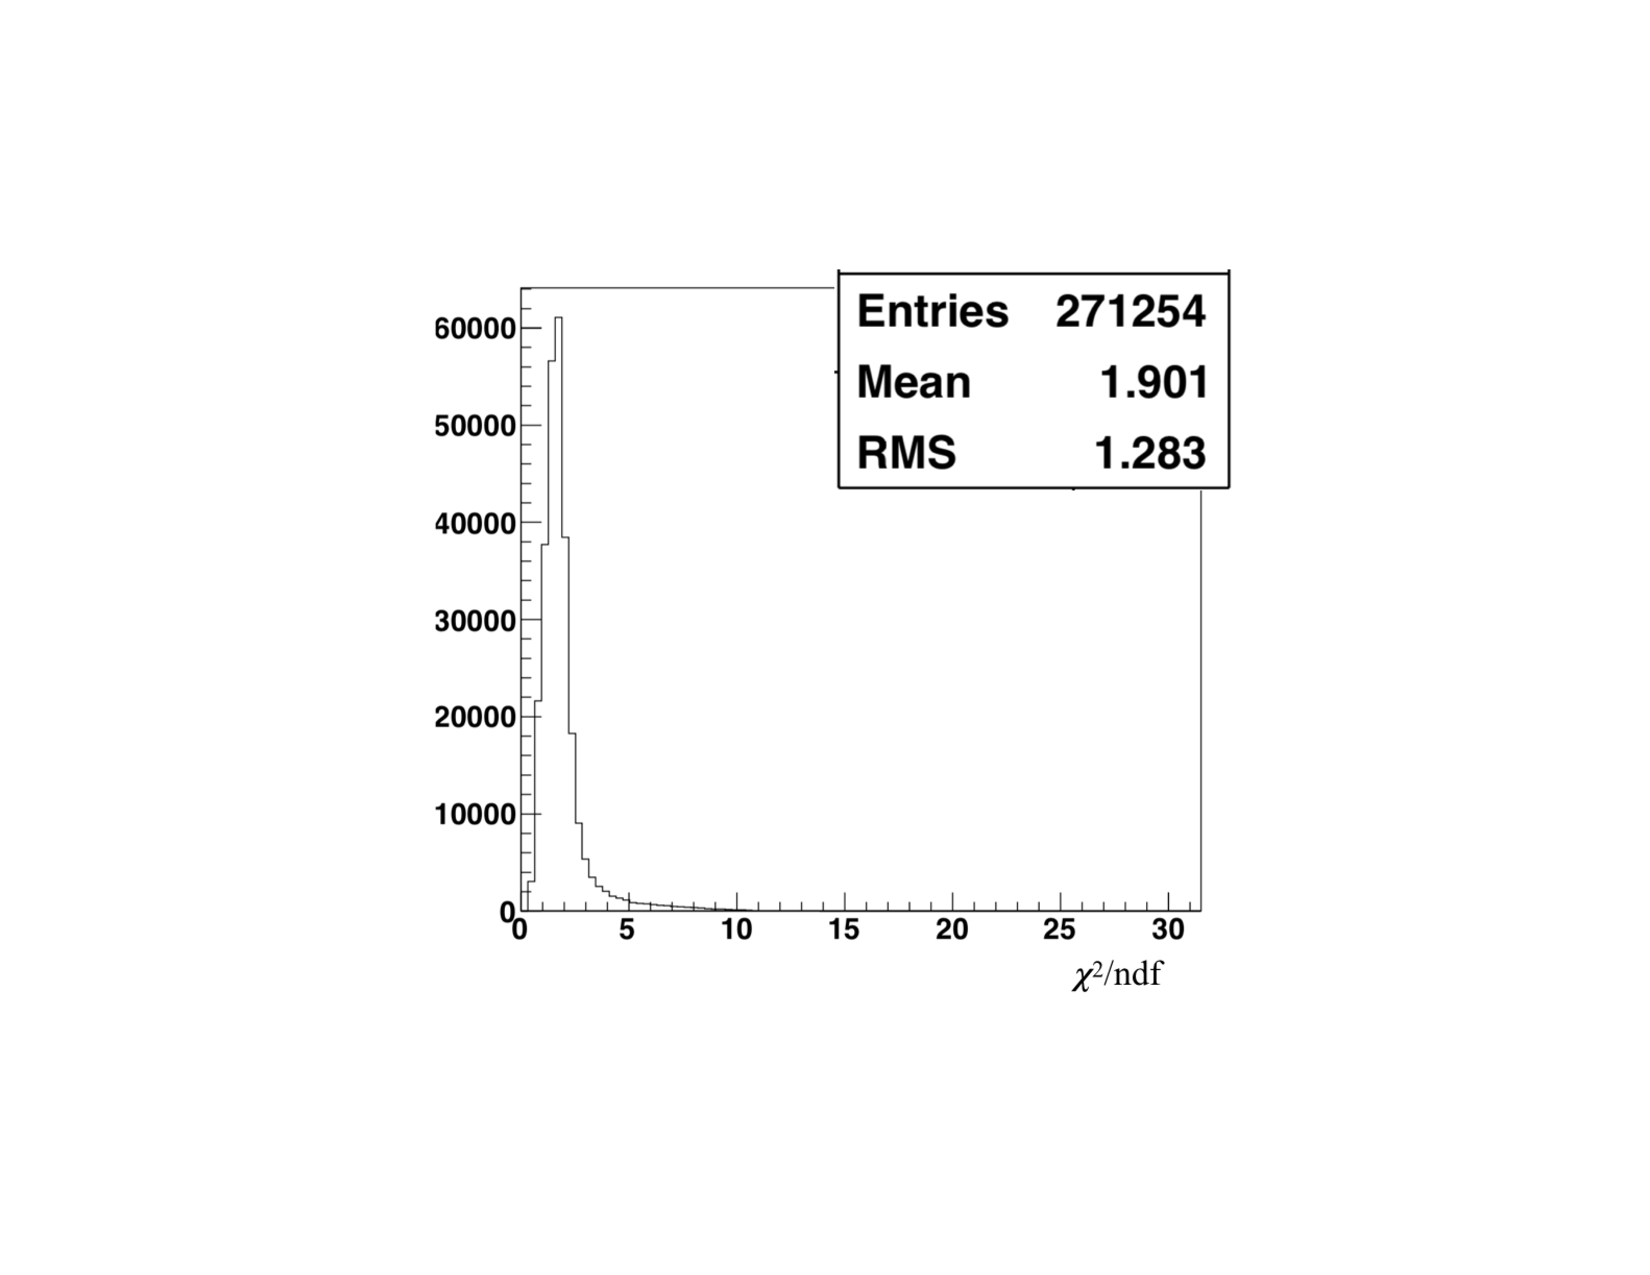
\includegraphics[width=0.5\textwidth, trim=5cm 4.5cm 5cm 4.5cm,
      clip]{trackChi2ndf}
    \caption{The reduced $\chi^2$ from alignment data tracks}
    \label{fig::trackChi2ndf}
  \end{figure}
  
\item The global number of tracks reconstructed.  Better alignment
  implies that more detectors can be associated with a track and therefore more
  tracks will be reconstructed.
\end{enumerate}

%\chapter{Measurement of the Left-Right Asymmetry in the Drell-Yan Process} 
\label{ch::leftright}
\ifpdf
\graphicspath{{Chapters/LeftRight/Figs/}}
\fi

This chapter goes over the analysis techniques and results from the 2015
transversely polarized Drell-Yan data taking.  The chapter begins by describing
the data collection setup and the event selection criteria followed by the
analysis techniques used to determine asymmetry amplitudes.  The analysis
techniques described are the standard transverse spin-dependent asymmetry
amplitude (TSA) analysis, Sec~\ref{sec::standTSA}, the double ratio analysis,
Sec~\ref{sec::doubleratio}, the $q_T$ weighted asymmetry analysis,
Sec~\ref{sec::qtweighting}, and finally the left-right asymmetry analysis,
Sec~\ref{sec::leftrighasym}.  All of these analyses are related in that they
measure TMD effects from the Drell-Yan process.  For this reason the event
selection and kinematical asymmetry binning will all be the same unless noted
otherwise.

\section{Data Sample} \label{sec::datasample}
The data sample is from the 2015 COMPASS Drell-Yan measurement where a 190 GeV/c
$\pi^-$ beam impinged on a transversely polarized NH$_3$ target.  The analysis
data is from July 8, through November 12 which is after an initial spectrometer
and beam commissioning phase.  The data is split into 9 periods lasting
approximated 2 weeks each, where each period consist of two sub-periods.  To
reduce systematic effects of acceptance and luminosity dependencies, the NH$_3$
target was split into two oppositely polarized cells with one cell polarized
vertically up and one cell polarized vertically down in the lab frame.  The
cells were separated by 20 cm and the polarization of both cells was flipped
between sub-periods.  A summary of the data taking from each period is shown in
Table ~\ref{tab::datataking}.

\begin{table}[h!t]
  \centering
  \begin{tabular}{ |c|c|c|c|c|c| }
    \hline Period& Sub-period& Polarization& First-Last run& Begin date& End
    date \\ \hline
    
    \multirow{2}{2em}{W07}& one& $\downarrow \uparrow$& 259363 - 259677& July
    9& July 15 \\ & two& $\uparrow \downarrow$& 259744 - 260016& July 16& July
    22 \\ \hline

    \multirow{2}{2em}{W08}& one& $\uparrow \downarrow$& 260074 - 260264& July
    23& July 29 \\ & two& $\downarrow \uparrow$& 260317 - 260565& July 29&
    August 5 \\ \hline

    \multirow{2}{2em}{W09}& one& $\downarrow \uparrow$& 260627 - 260852&
    August 5& August 12 \\ & two& $\uparrow \downarrow$& 260895 - 261496&
    August 12& August 26 \\ \hline

    \multirow{2}{2em}{W10}& one& $\uparrow \downarrow$& 261515 - 261761&
    August 26& September 1 \\ & two& $\downarrow \uparrow$& 261970 - 262221&
    September 4& September 9 \\ \hline

    \multirow{2}{2em}{W11}& one& $\downarrow \uparrow$& 262370 - 262772&
    September 11& September 22 \\ & two& $\uparrow \downarrow$& 262831 -
    263090& September 23& September 30 \\ \hline

    \multirow{2}{2em}{W12}& one& $\uparrow \downarrow$& 263143 - 263347&
    September 30& October 7 \\ & two& $\downarrow \uparrow$& 263386 - 263603&
    October 8& October 14 \\ \hline

    \multirow{2}{2em}{W13}& one& $\downarrow \uparrow$& 263655 - 263853&
    October 15& October 21 \\ & two& $\uparrow \downarrow$& 263926 - 264134&
    October 22& October 28 \\ \hline

    \multirow{2}{2em}{W14}& one& $\uparrow \downarrow$& 264170 - 264330&
    October 28& November 2 \\ & two& $\downarrow \uparrow$& 264429 - 264562&
    November 4& November 8 \\ \hline

    \multirow{2}{2em}{W15}& one& $\downarrow \uparrow$& 264619 - 264672&
    November 9& November 11 \\ & two& $\uparrow \downarrow$& 264736 - 264857&
    November 12& November 16 \\ \hline
    
  \end{tabular}
  \caption{COMPASS 2015 data taking periods}
  \label{tab::datataking}
\end{table}

\subsection{Stability Tests} \label{sec::stability}
To ensure the data analyzed were recorded during stable beam and spectrometer
conditions, stability of the analysis data was performed on a spill-by-spill and
run-by-run basis.  The data was recorded in runs with a maximum of 200 spills
per run and where one spill can have several thousand events.

\subsubsection{Bad Spill Analysis} To determine if a given spill is deemed
unstable several macro variables were averaged over the spill and compared to
neighboring spills.  These macro variables were chosen specifically to be
sensitive to the general stability conditions of the spectrometer and are listed
in the follower enumerated list Table~\ref{tab::badspillmacros}.  The starting
criteria for an event was two oppositely charged muons where a muon was defined
as having crossed 15 radiation lengths of material.

\begin{enumerate}
  \label{tab::badspillmacros}
\item number of beam particles divided by the number of events
\item number of beam particles divided by the number of primary vertices
\item number of hits per beam track divided by the number of beam particles
\item number of primary vertices divided by the number of events
\item number of outgoing tracks divided by the number of events
\item number of outgoing particles from a primary vertex divided by the number
  of primary vertices
\item number of outgoing particle from primary vertex divided by the number of
  events
\item number of outgoing particles from primary vertex divided by the number of
  events
\item number of hits from outgoing particles divided by the number outgoing
  particles
\item number of $\mu^+$ tracks divided by the number of events
\item number of $\mu^+$ tracks from primary vertex divided by the number of
  events
\item number of $\mu^-$ tracks divided by the number of events
\item number of $\mu^-$ tracks from primary vertex divided by the number of
  events
\item $\sum \chi^2$ of outgoing particles divided by the number of outgoing
  particles
\item $\sum \chi^2$ of all vertices divided by the number of all vertices in an
  event
\item Trigger rates (LASxLAS, OTxLAS, LASxMT)
\end{enumerate}

If the spectrometer was stable during a spill the average values from the
variables in Table~\ref{tab::badspilmacros} are expected to be constant from one
spill to the next.  To determine if a spill was recorded in unstable conditions
the spill of interest is compared with its neighboring 2500 spill occurring
before and after in time.  If the spill of interest is a specified sigma away
from any of the neighboring spills too many times, the spill of interest is mark
as a bad spill.  If a spill fails this bad spill criteria for any of the macro
variables in Table~\ref{tab::badspilmacros} the spill is deemed bad and not
included in the analysis.  The criteria for the sigma distance and number
times a spill crosses this distance to be deemed a bad are different for each
data taking period.  In addition to checking the nearest spills for each spill,
all the spills in a run are marked bad if the run it has less than 10 spills or
greater than 70\% bad spills.  Table~\ref{tab::badspillpercent} describes to
impact of the bad spill analysis on each period. \par

\subsubsection{Bad Run Analysis}
The stability of the spectrometer is also verified on run-by-run check in
parallel to the spill-by-spill check.  The run-by-run analysis compares
kinematic distributions and the average of these distributions per run to the
same kinematic distributions and averages from the other runs in a given period.
The kinematic distributions tested are: x$_{\mathrm{N}}$, x$_{\pi}$,
x$_{\mathrm{F}}$, q$_{\mathrm{T}}$, M$_{\mu\mu}$, P$_{\mu^+}$, P$_{\mu^-}$,
P$_{\gamma}$, P$_{\pi^-}$, and vertex x, y and z positions.  The quantities in
the run-by-run analysis are expected to influence the asymmetries
measured, however their distributions and averages are not expected to have
spin-influenced effects from the limited statistics in just a single run.  An
unbinned-Kolmogorov test (UKT) is performed to compare each distributions.  An
UKT test is made between all the runs in a given period and a run is marked bad
if it is incompatible with most of the runs in a period.  The comparison of mean
for each distribution from each run is made with the average from a given
period.  If one of the kinematical variables has an average more than five
standard deviations from the average within a period, the run is rejected.  The
results of the bad spill rejection after having already applied the bad spill
rejection are shown in Table~\ref{tab::badspillpercent}.

\begin{table}[h!t]
  \centering
  \label{tab::badspillpercent}
  \caption{Stability analysis rejection percentages}
  \begin{tabular}{ |c|c|c| }
    \hline \textbf{Period}& \textbf{Bad spill rejection}&
    \textbf{Bad spill and spill rejection} \\ \hline \hline
    
    W07& 11.79\%& 17.94\%\\ \hline
    W08& 18.00\%& 21.19\%\\ \hline
    W09& 14.76\%& 17.11\%\\ \hline
    W10& 15.88\%& 17.80\%\\ \hline
    W11& 22.49\%& 26.14\%\\ \hline
    W12& 12.71\%& 13.79\%\\ \hline
    W13& 22.32\%& 22.73\%\\ \hline
    W14& 8.91\%& 10.70\%\\ \hline
    W15& 3.94\%& 3.94\%\\ \hline

  \end{tabular}
\end{table}

\subsection{Event Selection} \label{sec::dy_eventselection}
The cuts in the event selection were chosen to ensure the event consisted of two
oppositely charged muons, so called dimuons, resulting from a pion collision in
the transversely polarized target.  The event selection was initial filtered
from miniDSTs to $\mu$DSTs using the criteria of at least two muons detected in
the spectrometer.  The cuts used in this analysis are described in the following
enumerated list where the event selection is performed on these $\mu$DSTs and
the events used come from the slot1 production.  A summary of the number of
events remaining after the last cuts is shown in Table~\ref{tab::EventTable}.

\begin{enumerate}
  \label{tab::cutdescrip}
\item Two oppositely charged particles from a common best primary vertex.  A
  primary vertex is defined as any vertex with an associated beam particle.  In
  case of multiple common primary vertices the best primary vertex was
  determined by CORAL tagging the vertex as best primary (PHAST method
  PaVertex::IsBestPrimary()).  In the case that CORAL did not tag any of the
  common vertices as the best primary the vertex with the smallest spatial
  $\chi^2$ value was used as the best primary vertex.
\item A dimuon trigger fired.  A dimuon trigger firing means there are at least
  two particles in coincidence in this event. The dimuon triggers used were a
  coincidence between two particles in the large angle spectrometer, LAS-LAS
  trigger, or a particle in the large angle spectrometer and a particle in the
  Outer hodoscope in the small angle spectrometer, LAS-Outer trigger.  The
  LAS-Middle trigger was used as a veto on beam decay muons where beam decay
  muons result from the decay of the beam pion, kaon or anti-proton into a muon.
  This beam decay muon can then be in coincidence with a positive muon from
  another decay or strong reaction in the target.  The LAS-Middle trigger was
  used a veto because this trigger was found to have many events
  resulting from a beam pion decaying to a muon.
\item Both particles are muons.  A muon was defined as having crossed 30
  radiation lengths of material between the particles first and last measured
  points.  This criteria has been previously determined to be effective at
  distinguishing between muons and hadrons.  In the data production no
  detectors were used from upstream of the hadron absorber so the absorber is
  not included in the determination of material crossed.
\item The first measured point for both particles is before 300 cm and the last
  measured point is after 1500 cm.  This cut ensures both particles have
  positions upstream of the first spectrometer magnet and downstream of the
  first muon filter.
\item The timing of both muons is defined.  This checks that the time relative
  to the trigger time is determined for both muons so further timing cuts can be
  performed.
\item Both muons are in time within 5 nanoseconds.  This track time for each
  muon is defined relative to the trigger time as in the previous cut.  The This
  cut helps rejected uncorrelated muons.
\item The muon track's spacial reduced $\chi^2$s are individually less than 10.
  This cut ensures track quality.
\item A validation that each muon crossed the trigger it was associated as
  having triggered.  This trigger validation cut was performed by extrapolating
  (PHAST Method PaTrack::Extrapolate()) each muon track back to the hodoscopes
  it fired and determining if the muon crossed the geometric acceptance of both
  hodoscopes.
\item The event does not occur in the bad spill or run list.  Many tests were
  performed to test the basic stability of the spectrometer and beam as
  described in section~\ref{sec::stability}.  The spills placed on the bad spill
  list were deemed to occur during unstable data taking conditions.
\item The Drell-Yan kinematics are physical.  That is x$_{\pi}$ and
  x$_{\mathrm{N}}$ are between 0 and 1 and x$_{\mathrm{F}}$ is between -1 and 1.
\item The transverse momentum of the virtual photon, q$_{\mathrm{T}}$ is between
  0.4 and 5.0 GeV/c.  The lower limit ensures azimuthal angular resolution is
  sufficient and the upper cut is minimal and further ensures the kinematic
  distributions are physically possible.
\item The vertex originated within the z-positions of the transversely polarized
  target cells defined by the target group (-294.5$<$ Z$_{\mathrm{vertex}}$
  $<$-239.3 for the upstream target or -219.5$<$ Z$_{\mathrm{vertex}}$ $<$-164.3
  cm for the downstream target).
\item The vertex is within the radius of the polarized target measured to be 1.9
  cm.
\end{enumerate}

\begin{figure}[h!t]
  \begin{adjustwidth}{-2cm}{}
    \begin{tabular}{ |c|c|c|c|c|c|c|c|c|c|c|c| }
      \hline \textbf{Cuts}& \textbf{W07}& \textbf{W08}& \textbf{W09}&
      \textbf{W10}& \textbf{W11}& \textbf{W12}& \textbf{W13}& \textbf{W14}&
      \textbf{W15} & \textbf{WAll} & \textbf{\% Remaining} \\ \hline

      All Data& 19410& 19184& 19654& 20707& 31371& 23563& 20561& 13154& 7697&
      175301& 100.00 \% \\ \hline
      
      Good Spills& 15947& 14899& 16217& 16895& 23041& 20184& 16026& 11796& 7422&
      142427& 81.70 \% \\ \hline

      0$<$ x$_{\pi}$ x$_N$ $<$1, -1$<$ x$_F$ $<$1& 15932& 14886& 16200& 16885&
      23022& 20171& 16013& 11794& 7414& 142317& 81.70 \% \\ \hline

      0.4$<$ q$_T$ $<$5(GeV/c)& 14342& 13385& 14609& 15239& 20667& 18101& 14365&
      10588& 6636& 127932& 60.75 \% \\ \hline

      Z Vertex within NH$_3$& 4256& 4024& 4330& 4552& 6369& 5503& 4411& 3130&
      2028& 38603& 15.05 \% \\ \hline

      Vertex Radius $<$ 1.9cm& 4175& 3950& 4257& 4474& 6252& 5414& 4334& 3078&
      1987& 37921& 12.21 \% \\ \hline
      
    \end{tabular}
    \caption{Event selection statistics for this analysis}
    \label{tab::EventTable}
  \end{adjustwidth}
\end{figure}

\subsection{Binning}
The asymmetries are measured in bins of x$_N$, x$_{\pi}$, x$_{\mathrm{F}}$,
q$_{\mathrm{T}}$, and M$_{\mu\mu}$.  Where x$_N$ and x$_{\pi}$ the momentum
fractions of the target nucleon and beam pion respectively, x$_{\mathrm{F}}$ =
x$_{\pi}$ - x$_N$, q$_{\mathrm{T}}$ is the transverse momentum of the virtual
photon and M$_{\mu\mu}$ is the invariant mass of the di-muon.  The binning was
determined by requiring equal statistical population in each kinematic bin.  In
addition, the asymmetries are determined in an integrated bin using all the
analysis data.  The analyzes binning limits are summarized in
Table~\ref{tab::binning}.

\begin{table}[h!t]
  \centering
  \begin{tabular}{ |c|c|c|c|c| }
    \hline \textbf{Kinematics}& \textbf{Lowest limit}& \textbf{Upper limit bin
      1}& \textbf{Upper limit bin 2}& \textbf{Upper limit bin 3}\\ \hline
    
    x$_N$& 0.0& 0.13& 0.19& 1.0\\ \hline x$_{\pi}$& 0.0& 0.40& 0.56&
    1.0\\ \hline x$_F$& -1.0& 0.22& 0.41& 1.0\\ \hline q$_T$ (GeV/c)& 0.4& 0.86&
    1.36& 5.0\\ \hline M$_{\mu\mu}$ (GeV/c$^2$)& 4.3& 4.73& 5.50& 8.5 \\ \hline
    
  \end{tabular}
  \caption{Analysis binning limits}
  \label{tab::binning}
\end{table}

\section{Transverse Spin-Dependent Asymmetries} \label{sec::standTSA}
This section describes the standard TSA analysis for which the results are
published in reference~\ref{compassDYpaper}.  The main motivation for this
analysis was to measure the sign of the Sivers function flip between Drell-Yan
and SIDIS using data from the same experimental setup for both processes.

As was noted in the event selection~\ref{tab::cutdescrip}, the data considered
are in the invariant mass range [4.3-8.5~{\gvcw}].
Fig.~\ref{fig::DY_InvariantMass} shows the invariant mass range from the 2015
COMPASS data with all cuts except the invariant mass range cut along with a fit
to show the background processes.  The fit is determine by Monte-Carlo data and
combinatorial background analysis.  The Monte-Carlo data simulated all hard
processes which decay to two oppositely charged muons and can be reconstructed
in the COMPASS spectrometer.  Combinatorial background analysis estimates the
background as $N_{combinatorial} = 2\sqrt{N_{\mu^+\mu^+}N_{\mu^-\mu^-}}$.  As
can be seen there are two background peaks.  The lower mass peak at about
3~{\gvcw} corresponds to J/$\Psi$ production and the mass peak at around
3.6~{\gvcw} corresponds to $\Psi$' production.  As can be seen, in the mass
range for all the analyses in this chapter, [4.3-8.5~{\gvcw}], the Drell-Yan
process dominates.  The background percentage was estimated to be below 4\% in
this analysis mass range.

\begin{figure}[h!t]
  \centering 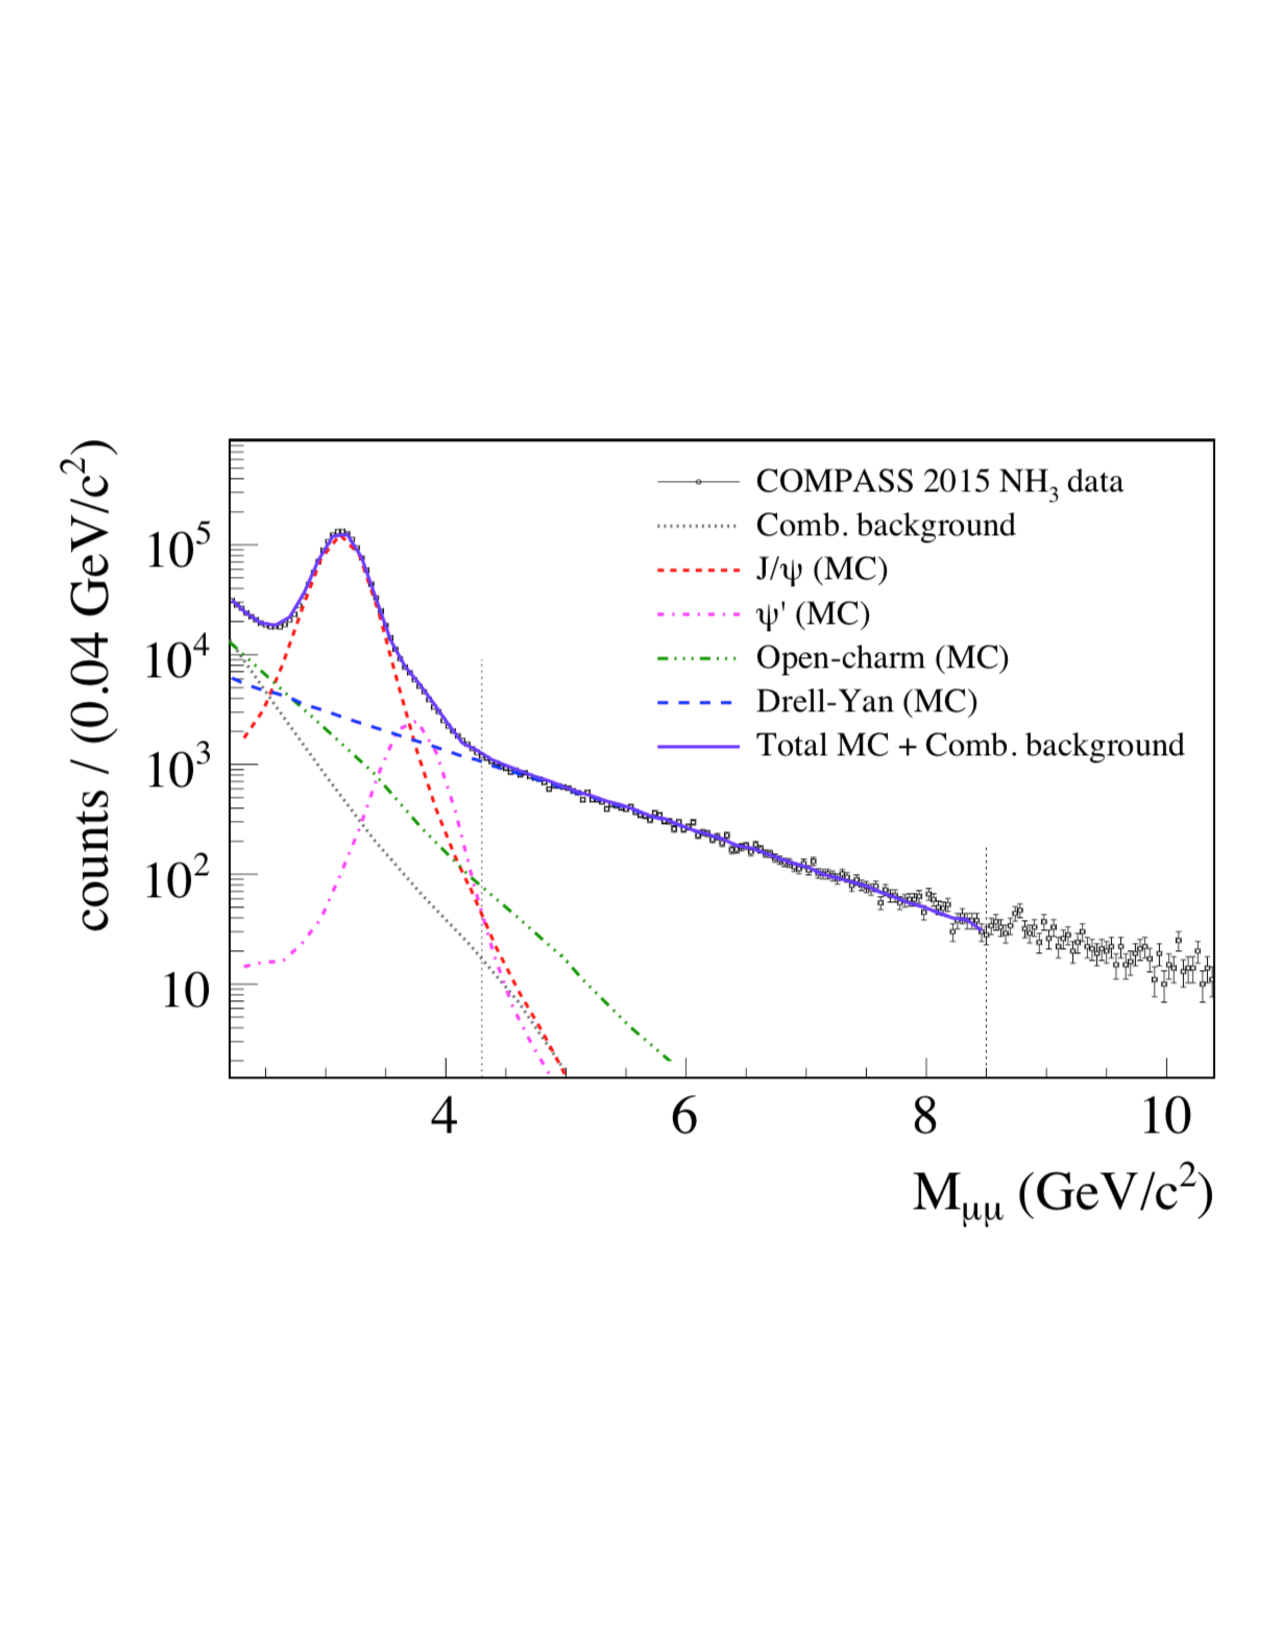
\includegraphics[width=0.6\textwidth,trim=1cm 7cm 1cm 7cm,
    clip]{DY_InvariantMass}
  \caption{The 2015 COMPASS invariant dimuon mass distribution and data fit.
    The data fit is from Monte-Carlo and combinatorial background analysis and
    is provided to show the background processes.  This image is taken
    from~\cite{compassDYpaper}.}
  \label{fig::DY_InvariantMass}
\end{figure}

Fig.~\ref{fig::DY_qT} shows the transverse virtual photon momentum, $q_T$,
distribution for this analysis.  The average $q_T$ for these analyses is
1.2~{\gvc} while the average $M_{\mu\mu}$ is 5.3~{\gvcw}.  As stated in
chapter~\ref{ch::theory}, the regime where TMD functions are the theoretical
model for parton distributions is when $q_T << M_{\mu\mu}$.  While the average
$q_T$ is less than the average $M_{\mu\mu}$, it is not excluded that the results
in this chapter are outside of the TMD limit.  Nevertheless the result present
are determined assuming the analyses are performed in the TMD regime.

\begin{figure}[h!t]
  \centering
  \begin{subfigure}{0.45\textwidth}
    \centering 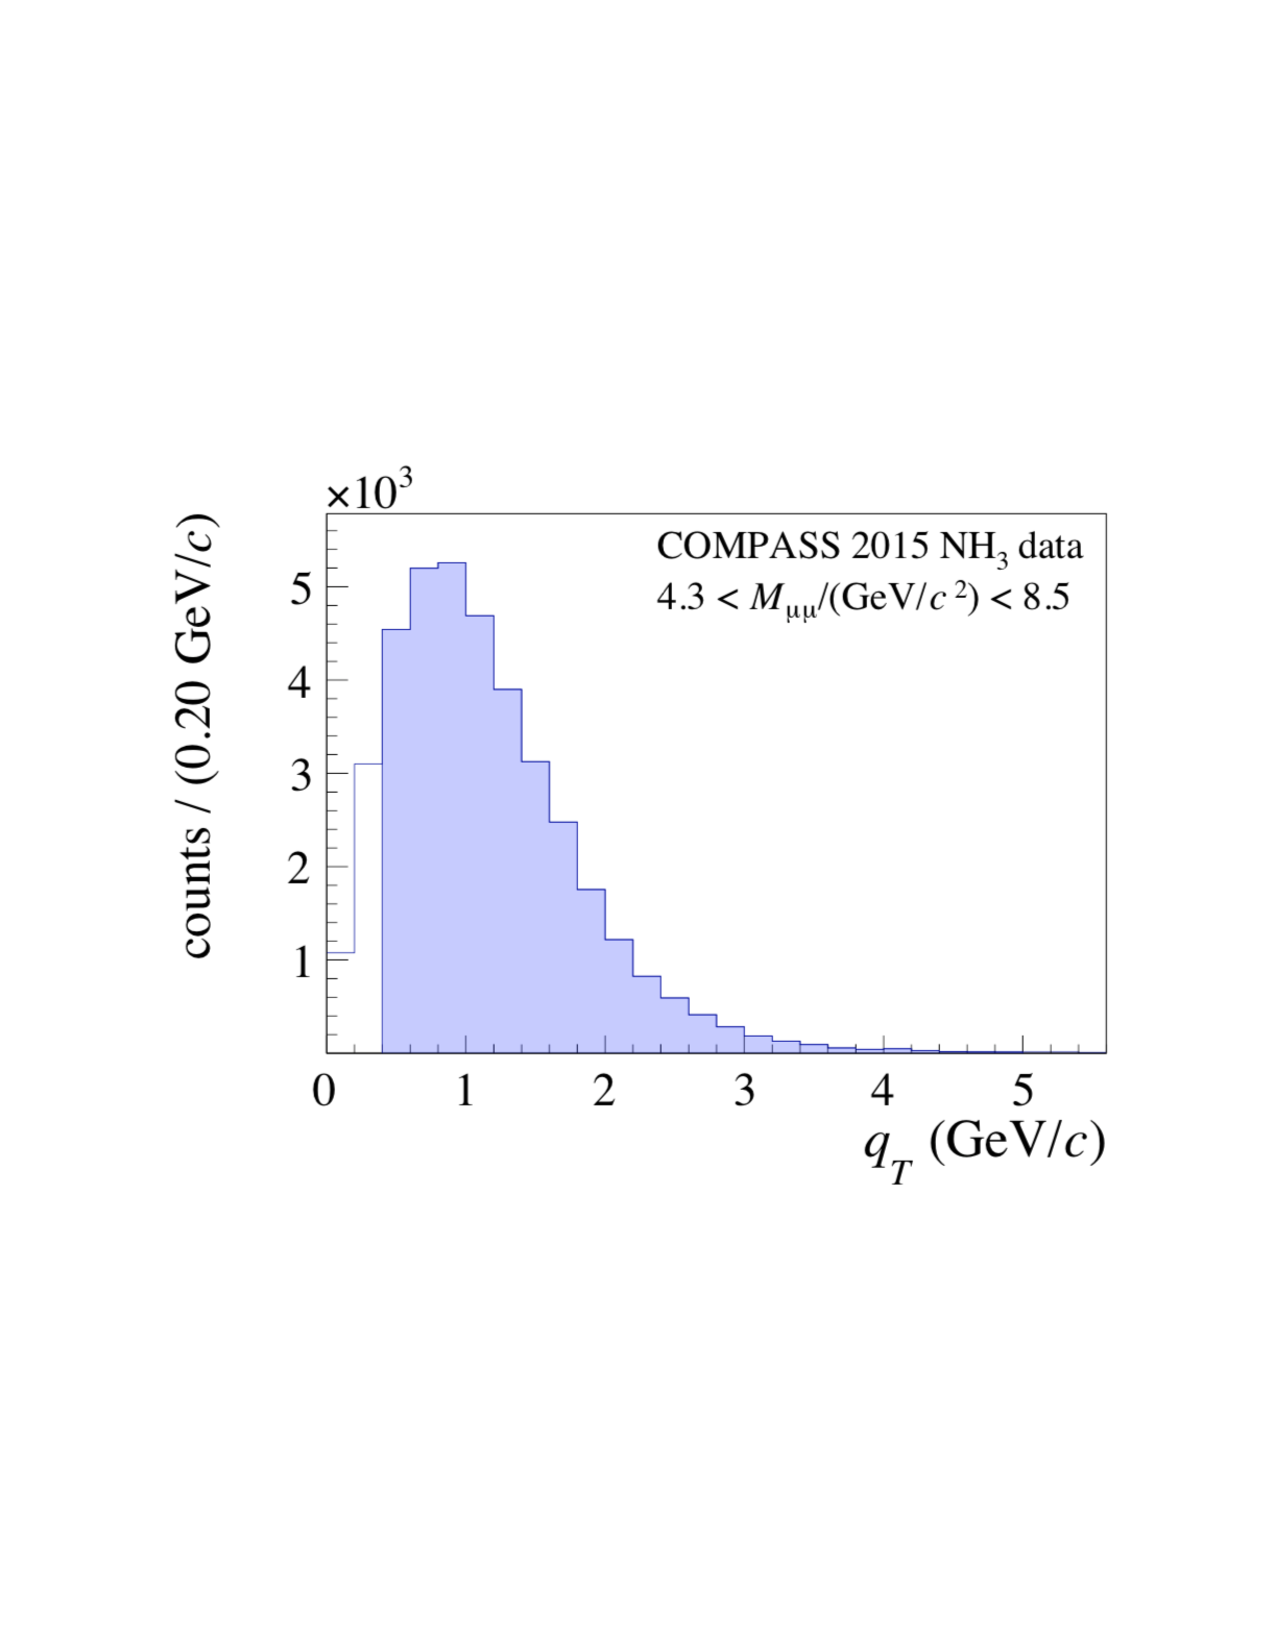
\includegraphics[width=\textwidth,trim=2cm 7.8cm 2cm 7cm,
      clip]{DY_qT}
    \caption{The $q_T$ distribution where the shaded regions shows the data used
      in the high mass analysis and the unshaded region shows the full
      distribution without a $q_T$ cut.  This image is taken
      from~\cite{compassDYpaper}.}
    \label{fig::DY_qT}
  \end{subfigure}
  \begin{subfigure}{.02\textwidth}
    
\includegraphics[width=\linewidth]{tmp3}
    \label{fig::tmp2}%
  \end{subfigure}
    \begin{subfigure}{0.48\textwidth}
    \centering 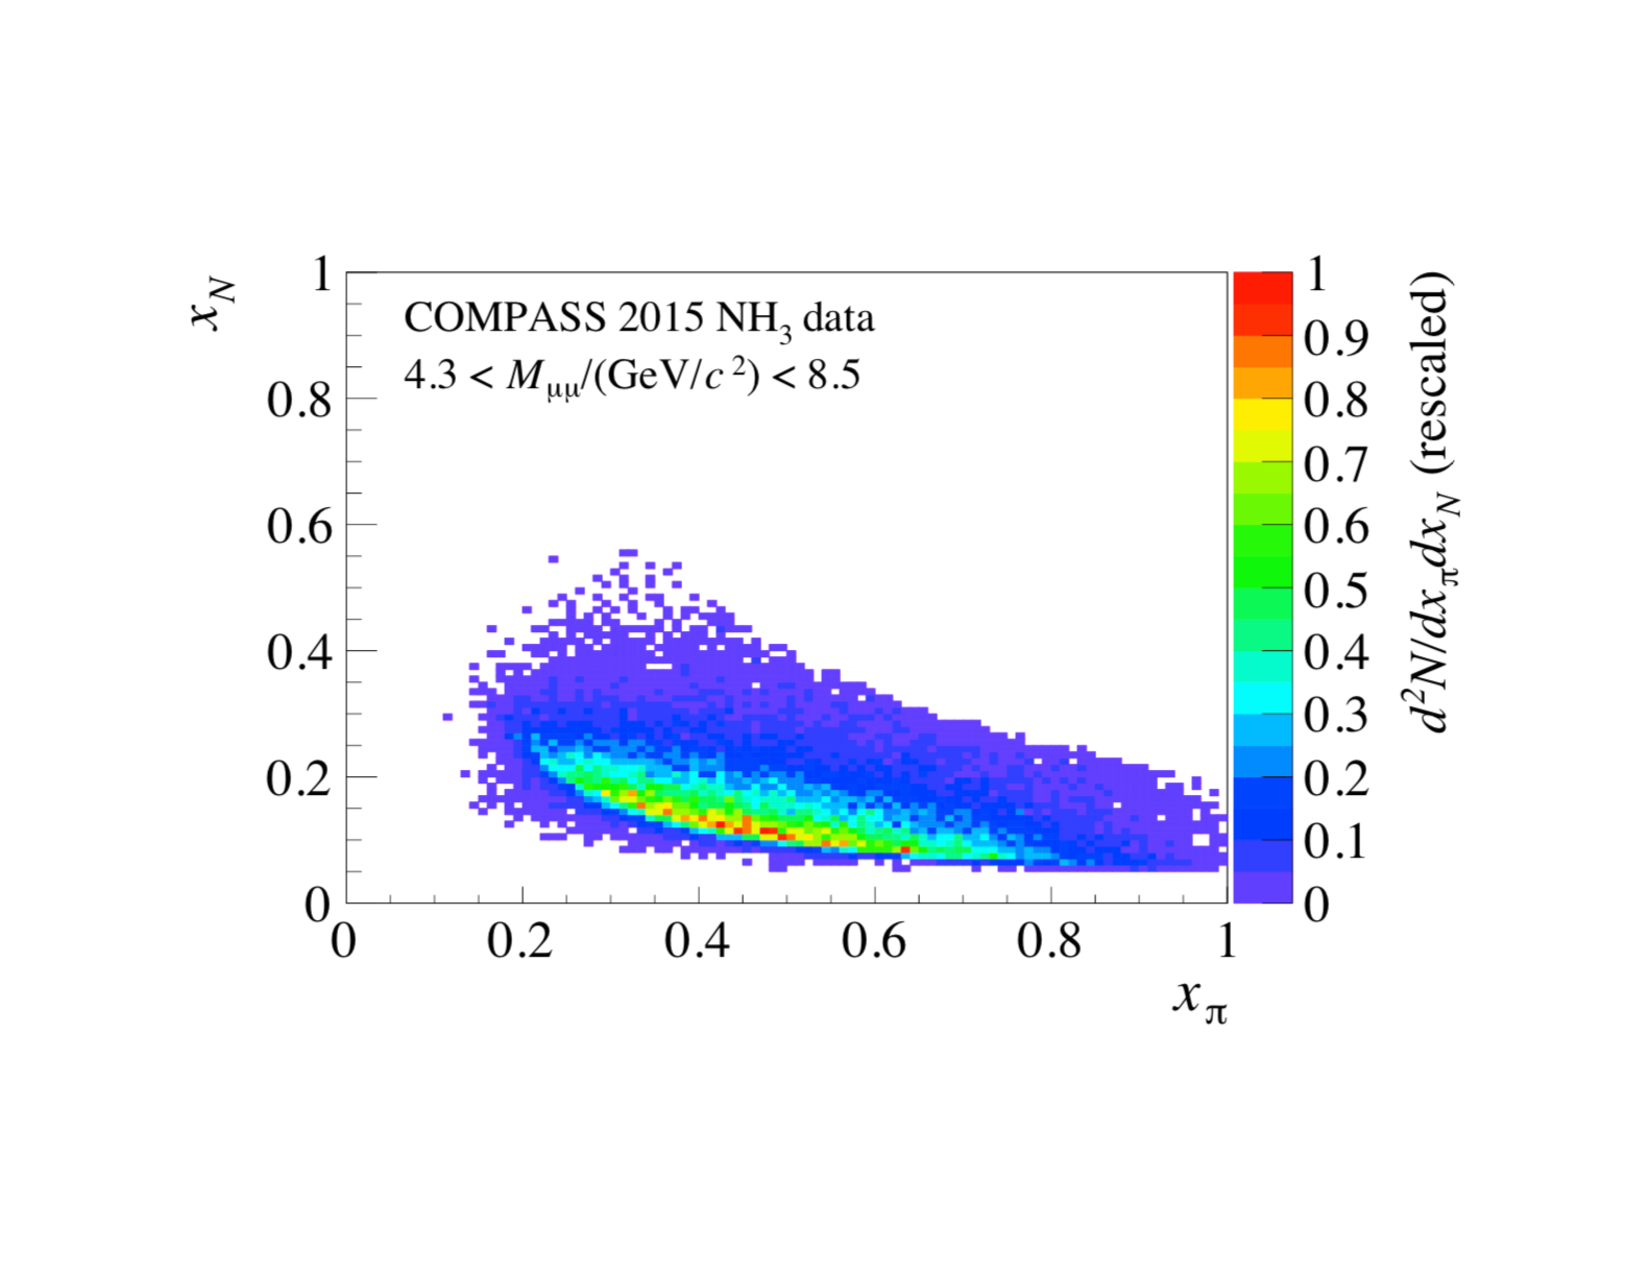
\includegraphics[width=\textwidth,trim=3.1cm 3.8cm 3.1cm
      3.8cm,clip]{DY_xPivxN}
    \caption{The 2-dimensional distribution of $x_{\pi}$ vs. $x_{N}$.  Both
      $x_{\pi}$ and $x_N$ are safely in their respective valence regions.  This
      image is taken from~\cite{compassDYpaper}.}
    \label{fig::DY_xPivxN}
  \end{subfigure}
\end{figure}

The distribution of $x_{\pi}$ versus $x_N$ is shown in
Fig.~\ref{fig::DY_xPivxN}.  The Bjorken-x of the proton, $x_N$, is almost
exclusively above 0.1 and as well Bjorken-x for the pion, $x_{\pi}$ is in it's
valence region.  For these reasons it is safe to say that the Drell-Yan reaction
studied these analyses is the result of the pion's anti-u-quark annihilating
with the proton's u-quark.

The results in this section are determined from an extended unbinned maximum
likelihood fit to the data.  The dilution and depolarization values are
determined on an event by event basis unlike the other analyses in this chapter.
The released integrated results for the leading order and sub-leading order TSAs
are shown in Fig.~\ref{fig::DY_intAsymAmps}.  The leading order TSAs are
non-zero with approximates significances of: 1 sigma for $A_T^{\sin(\phi_S)}$,
1.2 sigma for $A_T^{\sin(2\phi_{CS}+\phi_S)}$ and 2 sigma for
$A_T^{\sin(2\phi_{CS}-\phi_S)}$.

\begin{figure}[h!t]
  \centering 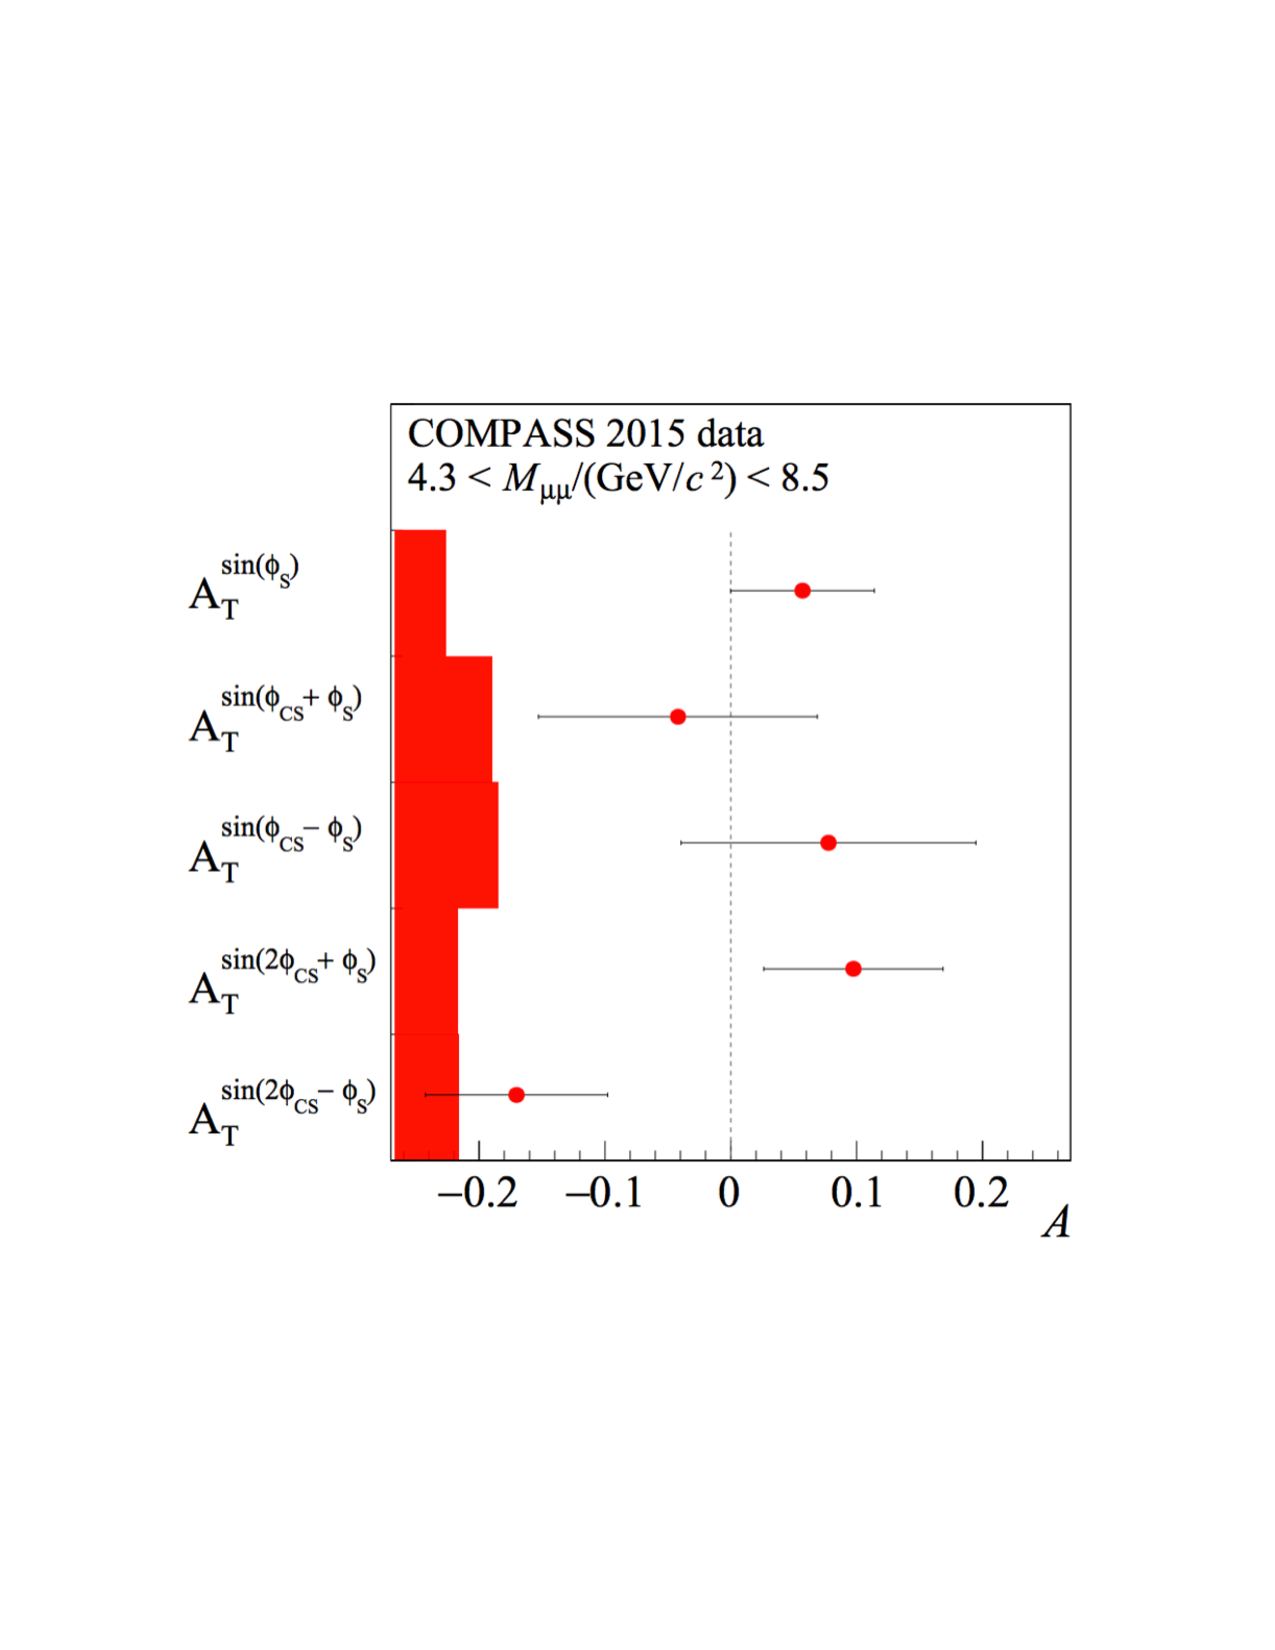
\includegraphics[width=0.43\textwidth,trim=3cm 7cm 3cm 6cm,
    clip]{DY_intAsymAmps}
  \caption{The integrated TSAs with statistical and systematic error bars.
    $A_T^{\sin(\phi_S)}$, $A_T^{\sin(2\phi_{CS}+\phi_S)}$, and
    $A_T^{\sin(2\phi_{CS}-\phi_S)}$ are leading order TSAs and
    $A_T^{\sin(\phi_{CS}+\phi_S)}$ and $A_T^{\sin(\phi_{CS}-\phi_S)}$ are
    sub-leading order TSAs.}
  \label{fig::DY_intAsymAmps}
\end{figure}

The comparison of the Sivers TSA, $A_T^{\sin(\phi_S)}$, with the expected sign
flip is shown in Fig.~\ref{fig::DY_Siv_signFlip}.  The positive solid theory
curves show the expected Sivers TSA assuming the Sivers function flips sign
between Drell-Yan and SIDIS.  The main difference in these three theory curves
is the $Q^2$ evolution technique used.  As can be seen the Sivers TSA is
compatible with the expected sign change.  However, the error bars on the Sivers
asymmetry amplitude are too large to conclusively distinguish between the three
theory curves or even to conclusively conclude on the sign change between
Drell-Yan and SIDIS.  That being said, the amplitude $A_T^{\sin(\phi_S)}$ is 2
sigma away from being incompatible with the sign flip.

\begin{figure}[h!t]
  \centering 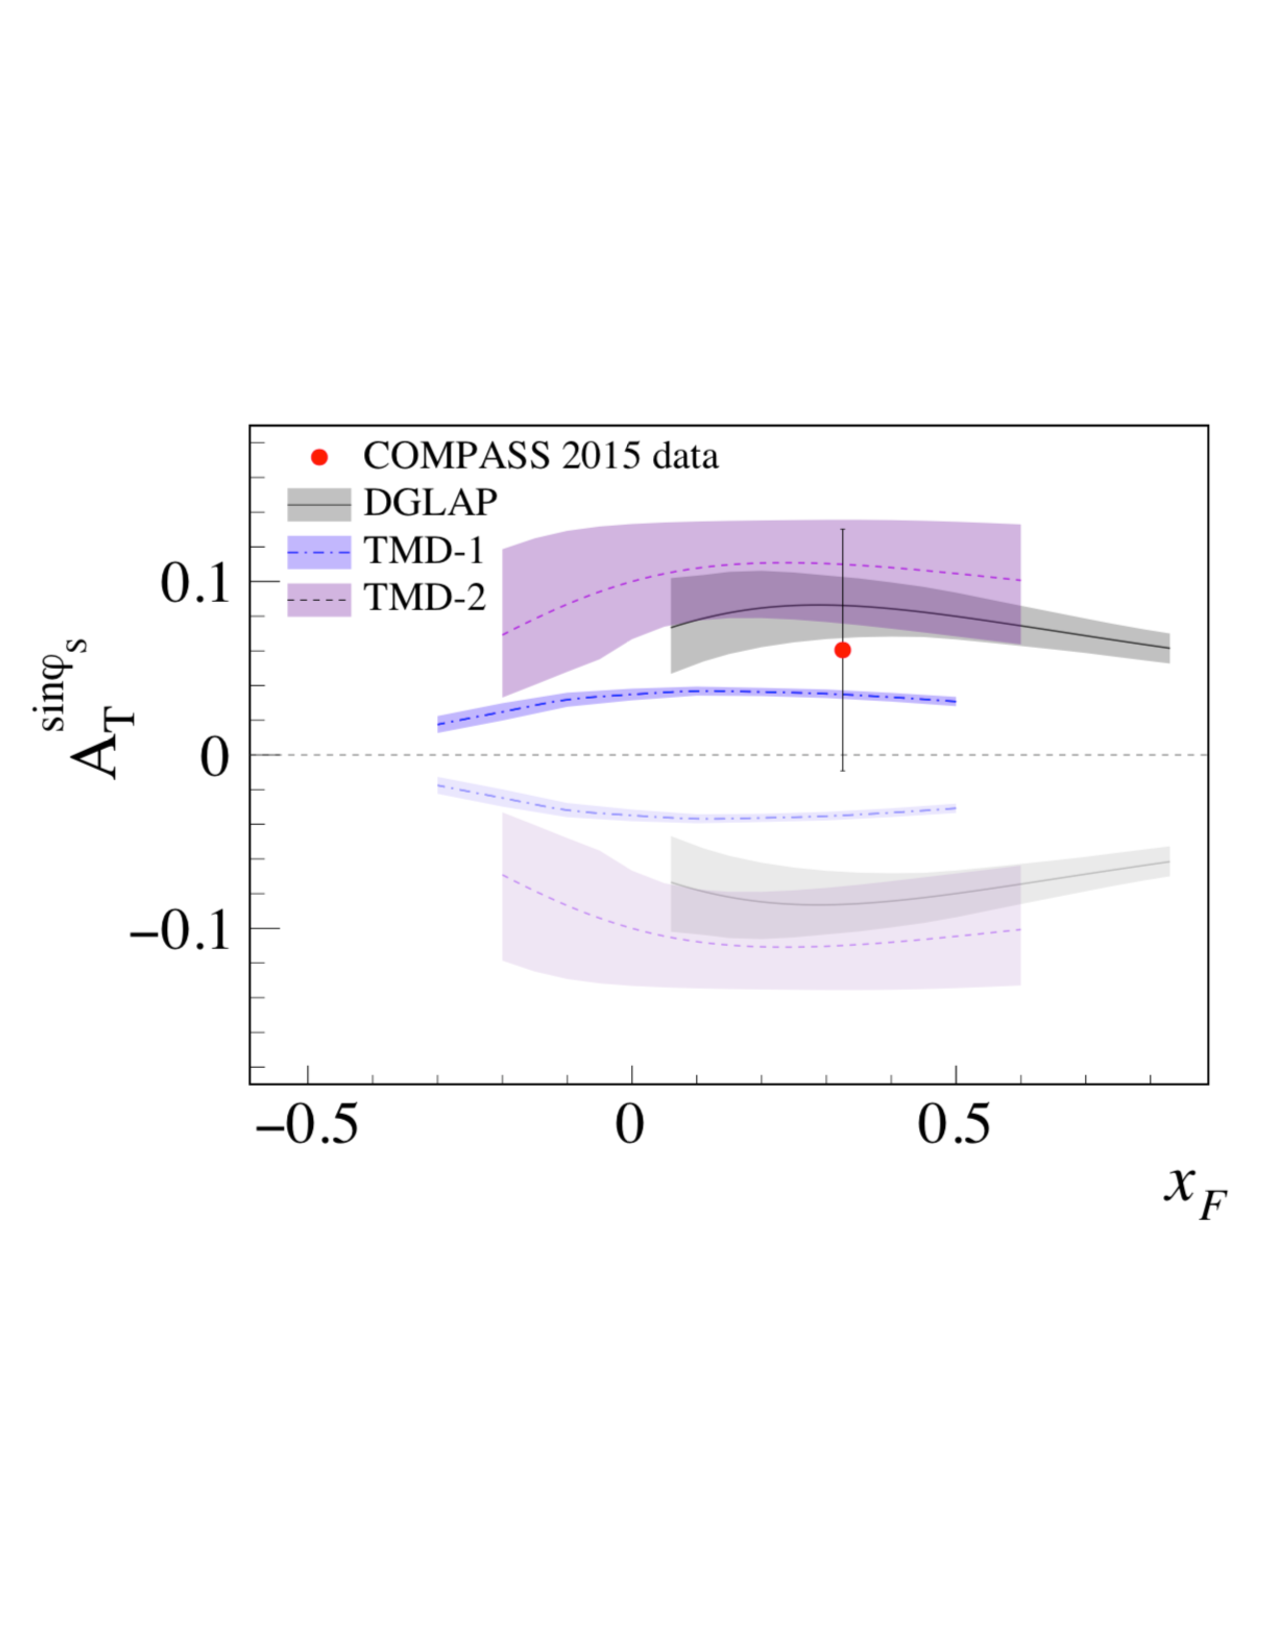
\includegraphics[width=0.6\textwidth, trim=0.5cm 7cm 0.5cm 7cm,
    clip]{DY_Siv_signFlip}
  \caption{The Sivers TSA along with theory curves for the expected sign change
    (sold curves) and without the sign change (opaque curves).  Theory curves
    and uncertainties are calculated using $Q^2$ evolution from
    DGLAP~\cite{Anselmino:2016uie}, TMD-1~\cite{Echevarria:2014xaa},
    TMD-2~\cite{Sun:2013hua}.  This image is taken from~\cite{compassDYpaper}.}
  \label{fig::DY_Siv_signFlip}
\end{figure}


\section{Extraction of Left-Right Asymmetries} \label{sec::leftrightasym}

This section goes over the analysis details for measuring the left-right
asymmetry from transversely polarized Drell-Yan data.  A theoretical
introduction showing how the left-right asymmetry is related to TMD PDFs and
related past result for this asymmetry are given in Sec~\ref{sec::lr_theory}.
In short the measured asymmetry can be defined as
\begin{equation}
  A_{lr} = \frac{\sigma_{Left} - \sigma_{Right}}{\sigma_{Left} +
    \sigma_{Right}}.
\end{equation}

There are many ways to determine the left-right asymmetry denoted as
A$_{\mathrm{N}}$.  The relevant techniques for the 2015 COMPASS setup are
described and compared to ensure confidence in the end results.
Sec.~\ref{sec::GeoMean} starts with a general introduction to the notations and
ideas used for all the asymmetry methods.

\subsection{Geometric Mean} \label{sec::GeoMean}
The number of physics counts, N, detected from any particular target can be
written as
\begin{equation}
  \label{equ::xsection}
  \mathrm{N} = \mathrm{L} * \sigma * \mathrm{a},
\end{equation}

\noindent
where L is the luminosity, $\sigma$ is the cross-section of such an event and a
is the acceptance.  In this formula the acceptance is a function of detector
efficiencies and the spectrometer acceptance.  In simple words, the number of
counts detected is the number of possible chances for an event to occur times
the probability for an event to occur and that the event will be detected.  To
get spin-dependent counts for the left-right asymmetry, the target, polarization
and left or right direction relative to the spin have to be included in the
counts.  Generically this can be written

\begin{equation}
  \label{equ::indexedCount}
  \mathrm{N}^{\uparrow(\downarrow)}_{\mathrm{cell},\mathrm{L(R)}} =
  \mathrm{a}^{\uparrow(\downarrow)}_{\mathrm{cell},\mathrm{spectrometer \;
      direction}} * \mathrm{L}^{\uparrow(\downarrow)}_{\mathrm{cell}} *
  \sigma_{\mathrm{L(R)}},
\end{equation}

\noindent
where $\uparrow(\downarrow)$ denotes the target polarization, cell is either
cell 1 for the upstream target cell or cell 2 for the downstream target cell,
L(R) is left(right) of the spin direction and spectrometer direction denotes
either the spectrometer Jura side or the Saleve side corresponding to where the
event was detected. \par

The most basic method to determine A$_{\mathrm{N}}$ per target cell is

\begin{equation}
  \label{equ::simpleAN}
  \mathrm{A}_{\mathrm{N}} = \frac{1}{\mathrm{P}}
  \frac{\mathrm{N}_{\mathrm{L}} -
    \mathrm{N}_{\mathrm{R}}}{\mathrm{N}_{\mathrm{L}} + \mathrm{N}_{\mathrm{R}}},
\end{equation}

\noindent
where the counts, N, are defined as Eq.~\ref{equ::xsection}, and P denotes the
fraction of polarized nucleons.  An intuitive picture of left and right defined
in the target frame is shown in Fig.~\ref{fig::leftright}.

\begin{figure}[h!t]
  \centering
  \includegraphics[width=0.6\textwidth, trim=7cm 6cm 7cm 7cm,clip]{leftright}
  \caption{The definition of the left plane (red) and right plane (green)
    defined from a target spin up configuration in the target frame}
  \label{fig::leftright}
\end{figure}

The previous definitions of the detected counts, Eq.~\ref{equ::indexedCount}
and Eq.~\ref{equ::xsection}, and therefore also Eq.~\ref{equ::simpleAN} all
depend on the spectrometer acceptance.  This is a problem because the
spectrometer acceptance can change with time and space and therefore can be
dependent on the physical kinematics which produced the event.  Such
dependencies can cause unphysical false asymmetries in the measurement of
A$_{\mathrm{N}}$ and must therefore be removed or must be included as systematic
effects. \par

Forming the geometric mean asymmetry is, however, a way to determine the
left-right asymmetry without acceptance effects from the spectrometer.  It is
defined as
\begin{equation}
  \label{equ::ANgeomean}
  \frac{1}{\mathrm{P}}\frac{\sqrt{N_{\mathrm{cell\;1(2),
          L}}^{\uparrow}N_{\mathrm{cell\;1(2), L}}^{\downarrow}} -
    \sqrt{N_{\mathrm{cell\;1(2), R}}^{\uparrow}N_{\mathrm{cell\;1(2),
          R}}^{\downarrow}} }{\sqrt{N_{\mathrm{cell\;1(2),
          L}}^{\uparrow}N_{\mathrm{cell\;1(2), L}}^{\downarrow}} +
    \sqrt{N_{\mathrm{cell\;1(2), R}}^{\uparrow}N_{\mathrm{cell\;1(2),
          R}}^{\downarrow}} },
\end{equation}

\noindent
where P represents the fraction of polarized
nucleons. Table~\ref{tab::ANnotations} summarizes the notations used throughout
this chapter.

\begin{table}[h!t]
  \centering
  \label{tab::ANnotations}
  \caption{Notations used in defining the left/right asymmetry}
  \begin{tabular}{ |c|c| }
    \hline
    \textbf{Notation}& \textbf{Description} \\
    \hline

    L(R) & virtual photon detected left(right) of spin \\ \hline
    Jura(Saleve) & spectrometer west(east) side \\ \hline
    cell 1(2)& up(down)stream target cell \\ \hline
    $\uparrow(\downarrow)$ & target cell polarized up(down) \\ \hline
    P& fraction of polarized target nucleons \\ \hline
    
  \end{tabular}
\end{table}

Equation~\ref{equ::ANgeomean} can be thought of simply as the normalized
difference of left minus right counts.  Left and right counts are determined
relative to the target spin directions and are defined as

\begin{equation}
  \label{equ::Defleftright}
  \begin{aligned}
    &\text{Left}: \hat{q}_T \cdot (\hat{S}_T \times \hat{P}_{\pi}) > 0 \\
    &\text{Right}: \hat{q}_T \cdot (\hat{S}_T \times \hat{P}_{\pi}) < 0, 
  \end{aligned}
\end{equation}

\noindent
where $\hat{q}_T$, $\hat{S}_T$ and $\hat{P}_{\pi}$ are unit vectors in the
target reference frame for the virtual photon transverse momentum, the target
spin and the beam pion momentum respectively.

Using Eq.~\ref{equ::indexedCount} for the definition of counts, the geometric
mean asymmetry is
\begin{equation}
  \label{equ::ANgeomean_expand}
  \frac{1}{\mathrm{P}}\frac{\kappa_{\mathrm{geomean}}
    \sqrt{\sigma_{L}\sigma_{L}} -
    \sqrt{\sigma_{R}\sigma_{R}}}{\kappa_{\mathrm{geomean}}
    \sqrt{\sigma_{L}\sigma_{L}} + \sqrt{\sigma_{R}\sigma_{R}}},
\end{equation}

\noindent
where $\kappa$ is a ratio of acceptances defined as
\begin{equation}
  \kappa_{\mathrm{geomean}} =
  \frac{\sqrt{\mathrm{a}^{\uparrow}_{\mathrm{cell\;1(2),Jura}}
      \mathrm{a}^{\downarrow}_{\mathrm{cell\;1(2),Saleve}}}}
       {\sqrt{\mathrm{a}^{\uparrow}_{\mathrm{cell\;1(2),Saleve}}
           \mathrm{a}^{\downarrow}_{\mathrm{cell\;1(2),Jura}}}}.
       \label{equ::accGeoMean}
\end{equation}

\noindent
Here the detection side of spectrometer is specified by looking down the beam
line as either Jura to mean left or Saleve to mean right.  These relations of
\"Jura is left\" and \"Saleve is right\" are only strictly true if the target
polarization is pointing straight up in the target frame.  In particular if the
beam particle and the target polarization do not make a right angle in the
laboratory frame this relation will no longer be strictly true but is an
approximation for ease of notation.

Relation~\ref{equ::ANgeomean_expand} is equal to A$_{\mathrm{N}}$ if $\kappa$ is
equal to one.  However as stated previously, time effects can vary $\kappa$ from
unity. These effects are estimated through false asymmetry analysis and included
in the systematic error bars described in section~\ref{sec::systematics}.
Equation~\ref{equ::ANgeomean} is therefore to a good approximation an acceptance
free method to determine A$_{\mathrm{N}}$.  It is also defined for the upstream
and downstream cells independently and therefore can be used as a consistency
check between the two target cells.

The statistical uncertainty of the geometry mean is
\begin{equation}
  \frac{1}{\mathrm{P}}
  \frac{
    \sqrt{
      N_{\mathrm{L}}^{\uparrow}N_{\mathrm{L}}^{\downarrow}
      N_{\mathrm{ R}}^{\uparrow}N_{\mathrm{R}}^{\downarrow}
    }
  }{
    \Big( \sqrt{N_{\mathrm{L}}^{\uparrow}N_{\mathrm{L}}^{\downarrow}} +
    \sqrt{N_{\mathrm{R}}^{\uparrow}N_{\mathrm{R}}^{\downarrow}} \Big)^2
  }
  \sqrt{
    \frac{1}{N_{\mathrm{L}}^{\uparrow}} +
    \frac{1}{N_{\mathrm{L}}^{\downarrow}} +
    \frac{1}{N_{\mathrm{R}}^{\uparrow}} +
    \frac{1}{N_{\mathrm{R}}^{\downarrow}}
  } \quad,
\end{equation}

\noindent
which reduces to $\frac{1}{\mathrm{P}}\frac{1}{\sqrt{\mathrm{N}}}$ in the case
of equal statistics in each direction from each target cell polarization.

\subsection{Two-Target Geometric Mean} \label{sec::TwoTargGeoMean}
As described in section~\ref{sec::datasample} COMPASS had two oppositely
polarized target cells in 2015.  The previous geometric mean asymmetry, however,
determined an A$_{\mathrm{N}}$ per target.  It is desirable from a statistical
point of view, however, to determine one A$_{\mathrm{N}}$ from the 2015 COMPASS
setup.  It is also desirable for comparison purposes to determine
A$_{\mathrm{N}}$ using all the information from the 2015 COMPASS setup.  This
can be accomplished by modifying the geometric mean to add both target cells as
follows

\begin{equation}
  \label{equ::AN4TargGeomean}
  \frac{1}{\mathrm{P}}
  \frac{
    \sqrt[4]{
      N_{\mathrm{cell\;1,L}}^{\uparrow}N_{\mathrm{cell\;1, L}}^{\downarrow}
      N_{\mathrm{cell\;2,L}}^{\uparrow}N_{\mathrm{cell\;2, L}}^{\downarrow}
    } -
    \sqrt[4]{
      N_{\mathrm{cell\;1,R}}^{\uparrow}N_{\mathrm{cell\;1, R}}^{\downarrow}
      N_{\mathrm{cell\;2,R}}^{\uparrow}N_{\mathrm{cell\;2, R}}^{\downarrow}
    }
  }{
    \sqrt[4]{
      N_{\mathrm{cell\;1,L}}^{\uparrow}N_{\mathrm{cell\;1, L}}^{\downarrow}
      N_{\mathrm{cell\;2,L}}^{\uparrow}N_{\mathrm{cell\;2, L}}^{\downarrow}
    } +
    \sqrt[4]{
      N_{\mathrm{cell\;1,R}}^{\uparrow}N_{\mathrm{cell\;1, R}}^{\downarrow}
      N_{\mathrm{cell\;2,R}}^{\uparrow}N_{\mathrm{cell\;2, R}}^{\downarrow}
    }
  }.
\end{equation}

As in the basic geometric mean asymmetry, section~\ref{sec::GeoMean}, left and
right are determined relative to the spin direction of the target as in
Eq.~\ref{equ::Defleftright}.  Again using Eq.~\ref{equ::indexedCount} for the
definition of counts, the two target geometric mean asymmetry,
Eq.~\ref{equ::AN4TargGeomean}, can be written as
\begin{equation}
  \frac{1}{\mathrm{P}}
  \frac{
    \kappa_{\mathrm{two-target}} \sqrt[4]{\sigma_{L}\sigma_{L}\sigma_{L}\sigma_{L}} -
    \sqrt[4]{\sigma_{R}\sigma_{R}\sigma_{R}\sigma_{R}}
  }{
    \kappa_{\mathrm{two-target}} \sqrt[4]{\sigma_{L}\sigma_{L}\sigma_{L}\sigma_{L}} +
    \sqrt[4]{\sigma_{R}\sigma_{R}\sigma_{R}\sigma_{R}}
  },
\end{equation},

\noindent
where now $\kappa_{\mathrm{two-target}}$ is the ratio of acceptances from all
targets and polarizations.  This inclusive acceptance ratio is defined as
\begin{equation}
  \label{equ::acc4TargGeoMean}
  \kappa_{\mathrm{two-target}} =
  \frac{
    \sqrt[4]{
      \mathrm{a}^{\uparrow}_{\mathrm{cell\;1,Jura}}
      \mathrm{a}^{\downarrow}_{\mathrm{cell\;1,Saleve}}
      \mathrm{a}^{\uparrow}_{\mathrm{cell\;2,Jura}}
      \mathrm{a}^{\downarrow}_{\mathrm{cell\;2,Saleve}}}
  }{
    \sqrt[4]{
      \mathrm{a}^{\uparrow}_{\mathrm{cell\;1,Saleve}}
      \mathrm{a}^{\downarrow}_{\mathrm{cell\;1,Jura}}
      \mathrm{a}^{\uparrow}_{\mathrm{cell\;2,Saleve}}
      \mathrm{a}^{\downarrow}_{\mathrm{cell\;2,Jura}}}
  }.
\end{equation}

\noindent
In this case the acceptance ratio is expected to vary less with time and
therefore be closer to unity than the normal geometric mean acceptance ratio,
Eq.~\ref{equ::accGeoMean}.  This is a consequence of having the different target
cells oppositely polarized.  Rewriting Eq.~\ref{equ::acc4TargGeoMean} with
sub-period superscripts instead of target polarization superscripts

\begin{equation}
  \label{equ::acc4TargGeoMean_subperiod}
  \kappa_{two-target} = \frac{
    \sqrt[4]{
      \mathrm{a}^{a}_{\mathrm{cell\;1,Jura}}
      \mathrm{a}^{b}_{\mathrm{cell\;1,Saleve}}
      \mathrm{a}^{b}_{\mathrm{cell\;2,Jura}}
      \mathrm{a}^{a}_{\mathrm{cell\;2,Saleve}}}
  }{
    \sqrt[4]{
      \mathrm{a}^{a}_{\mathrm{cell\;1,Saleve}}
      \mathrm{a}^{b}_{\mathrm{cell\;1,Jura}}
      \mathrm{a}^{b}_{\mathrm{cell\;2,Saleve}}
      \mathrm{a}^{a}_{\mathrm{cell\;2,Jura}}}
  },
\end{equation}

\noindent
where sub-period $a$ is with the upstream target polarized up and the downstream
target polarized down and vise versa for sub-period $b$.  From
Eq.~\ref{equ::acc4TargGeoMean_subperiod} it is more evident that the acceptance
ratio terms for sub-period $b$ are reciprocal to the terms for sub-period $a$
and therefore the acceptance ratio is expected to be more stably close to unity.

Finally the statistical uncertainty of the two target geometric mean is
\begin{equation}
  \frac{1}{\mathrm{P}}
  \frac{\text{LR}}{\Big( \text{L+R} \Big)^2}
  \sqrt{
    \sum_{\mathrm{cell}}\sum_{\mathrm{polarization}}
    \Big(
    \frac{1}{N_{\mathrm{cell,L}}^{\mathrm{polarization}}}
    +
    \frac{1}{N_{\mathrm{cell,R}}^{\mathrm{polarization}}}
    \Big)
  } \quad,
\end{equation}

\noindent
where L can be thought of as the left counts and equals to
$\sqrt[4]{N_{\mathrm{cell\;1,L}}^{\uparrow}N_{\mathrm{cell\;1,
      L}}^{\downarrow}N_{\mathrm{cell\;2,L}}^{\uparrow}N_{\mathrm{cell\;2,
      L}}^{\downarrow}}$ and R can be thought of as the right counts and equals
$\sqrt[4]{N_{\mathrm{cell\;1,R}}^{\uparrow}N_{\mathrm{cell\;1,
      R}}^{\downarrow}N_{\mathrm{cell\;2,R}}^{\uparrow}N_{\mathrm{cell\;2,
      R}}^{\downarrow}}$.  The statistical uncertainty for the two target
geometric mean also reduces to $\frac{1}{\mathrm{P}}\frac{1}{\sqrt{\mathrm{N}}}$
in the case of equal statistic populations in each direction and target
polarization.


\section{Systematic Studies} \label{sec::systematics}
Several tests were performed to estimate the systematic uncertainty of the
left-right asymmetry.  The systematic errors are determined by adding all
non-zero systematic uncertainties in quadrature.  The impact from each source of
systematic error is summarized in Tab.~\ref{tab::sysError}.

\subsection{Period Compatibility (Time Dependence)}
The asymmetries calculated for each time period in each kinematic bin are shown
in Fig.~\ref{fig::allPhysBinned4Targ}.

\begin{figure}[h!t]
  \begin{center}
    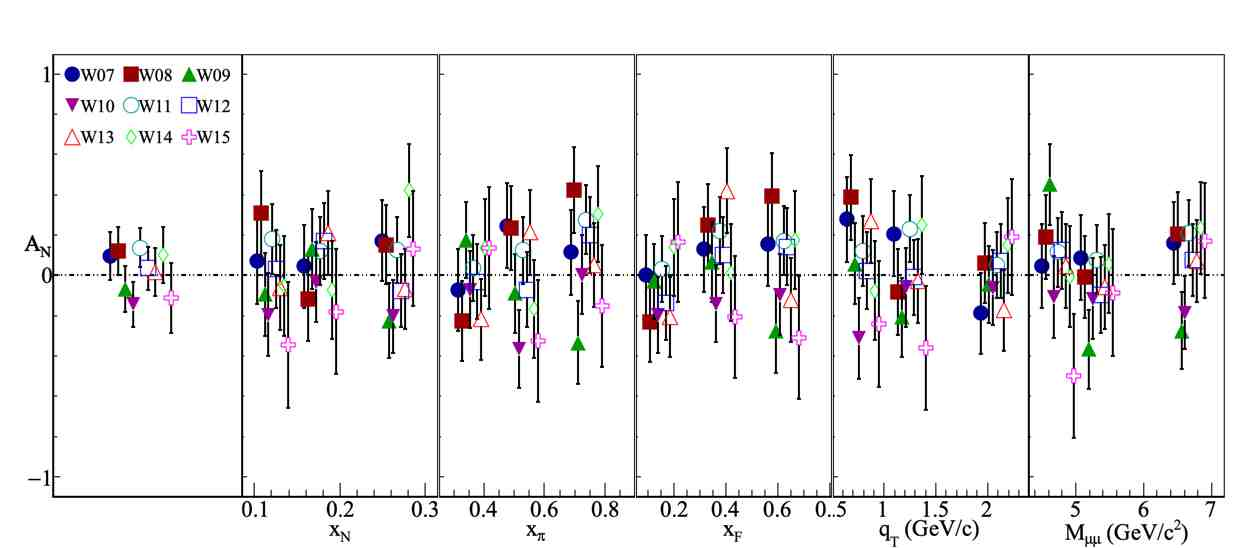
\includegraphics[width=\textwidth]{allPhysBinned4Targ}
    \caption{A$_{\mathrm{N}}$ determined for each period}
    \label{fig::allPhysBinned4Targ}
  \end{center}
\end{figure}

\noindent
By eye the asymmetry fluctuations appear to be statistically compatible.  To
quantify the compatibility of the asymmetries between the periods, a pull
distribution is formed.  The pull value is defined as

\begin{equation}
  \label{eq::pull}
  \Delta\mathrm{A}_i =
  \frac{
    \mathrm{A}_i - \langle \mathrm{A} \rangle
  }{
    \sqrt{
      \sigma^2_{\mathrm{A}_i} - \sigma^2_{\langle \mathrm{A} \rangle}
    }
  },
\end{equation}

\noindent
and is determined for each period and kinematic bin.  There are therefore 3
(number of bins) x 5 (number of kinematics) x 9 (number of periods) = 135
entries in the pull distribution. This distribution is shown in
Fig.~\ref{fig::pull4Targ} along with a Gaussian fit.  If the asymmetries all
come from the same parent distribution then due to the central limit theorem the
pull distribution will be a Gaussian distribution with zero mean and unit
variance.  The discrepancy of the pull distribution from a standard Gaussian
distribution is used to determine a systematic error as

\begin{equation}
  \label{equ::sysErrorPull}
  \frac{\sigma_{\mathrm{systematic}}}{\sigma_{\mathrm{statistical}}} =
  \sqrt{|\sigma^2_{\mathrm{pull}} - 1|} + \frac{\mu_{\mathrm{pull}}}{2}.
\end{equation}

\begin{figure}[h!t]
  \begin{center}
    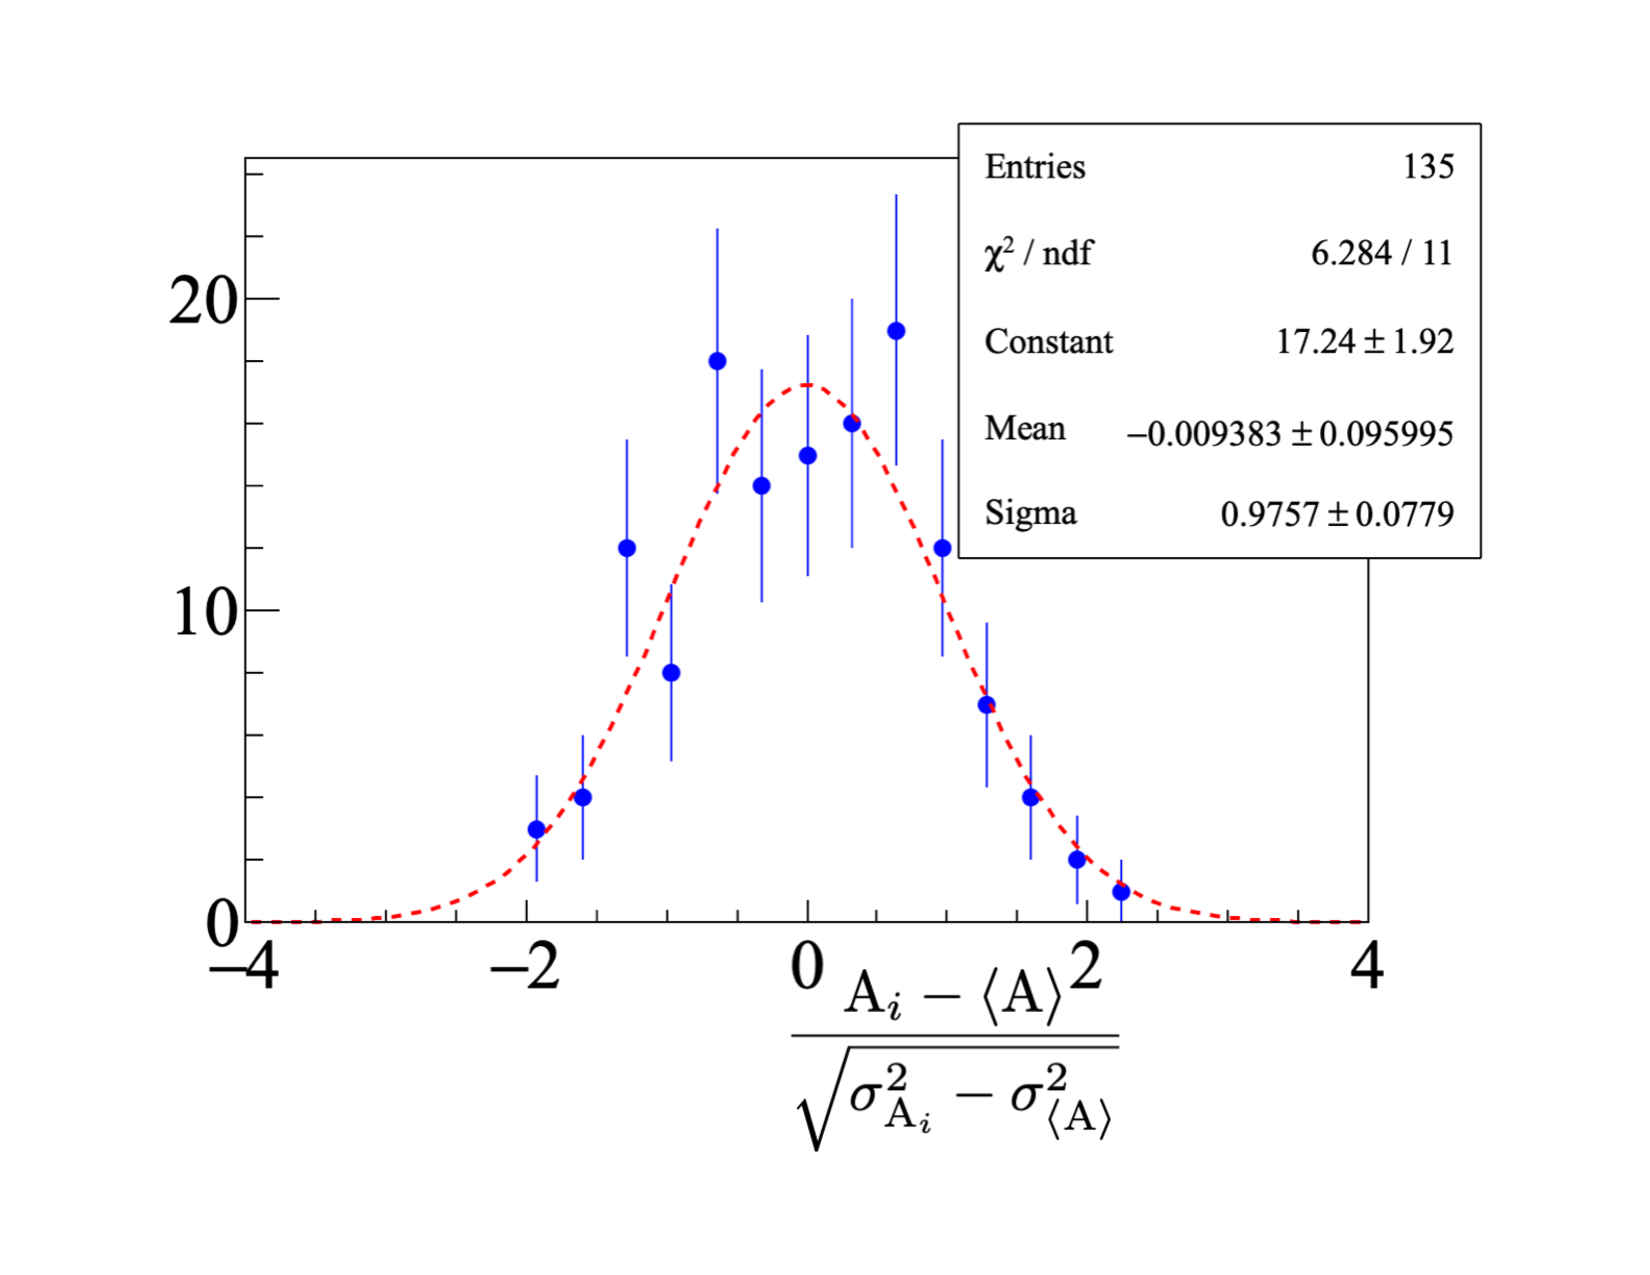
\includegraphics[width=0.8\textwidth, trim=0cm 0cm 0cm 2cm,clip]{pull4Targ}
    \caption{Pull distribution from the two target geometric mean}
    \label{fig::pull4Targ}
  \end{center}
\end{figure}

\noindent
As the asymmetries in different kinematic bins are formed using the same data
set the asymmetries between kinematic binning are correlated.  For this reason
an uncorrelated pull distribution is also formed for each kinematic bin and also
compared with a standard Gaussian distribution.  These distributions are shown
in Fig.~\ref{fig::allPhysPulls4Targ} and the results of the Gaussian fit are
shown in Fig.~\ref{fig::allPhysPulls4Targ_fit}.  For these uncorrelated pull
distributions there are now only 3 (number of bins) x 9(number of periods) = 27
entries in each kinetically binned pull distributions and only 9 (number of
periods) bins in the integrated pull distribution.

\begin{figure}[h!t]
  \begin{center}
    \includegraphics[width=\textwidth, trim=0cm 5cm 0cm 4cm,
      clip]{allPhysPulls4Targ}
    \caption{Uncorrelated pull distributions}
    \label{fig::allPhysPulls4Targ}
  \end{center}
\end{figure}

\begin{figure}[h!t]
  \begin{center}
    \includegraphics[width=\textwidth, trim=0.2cm 9cm 0.2cm 10cm,
      clip]{allPhysPulls4Targ_fit}
    \caption{Results of Gaussian fit for the uncorrelated pull distributions}
    \label{fig::allPhysPulls4Targ_fit}
  \end{center}
\end{figure}

Even though the Gaussian fits did not give exactly a standard Gaussian, the fit
parameters are well compatible with a standard Gaussian within the errors of the
fit.  Therefore no systematic error was assigned due to incompatibility of the
periods.

\subsection{False Asymmetries}
\subsubsection{Acceptance From False Asymmetries}
As was pointed out in Sec.~\ref{sec::GeoMean} and
Sec.~\ref{sec::TwoTargGeoMean}, the asymmetry measurement assumes the acceptance
does not change with time and therefore the acceptance ratios
Eq.~\ref{equ::accGeoMean} and Eq.~\ref{equ::acc4TargGeoMean} are unitary.  Any
deviation from a unitary acceptance ratio is estimated with a false asymmetry
and is taken as a systematic error.  To determine if acceptance
does change with time, a false asymmetry is calculated where the only way the
false asymmetry could be non-zero is if acceptance changes with time.  This
false asymmetry for the two target geometric mean is

\begin{equation}
  \label{equ::falseAcc}
  \begin{split}
    A_{\mathrm{N,False}} &= 
    \frac{1}{\mathrm{P}}
    \frac{
      \sqrt[4]{
        N_{\mathrm{cell\;1,R}}^{\uparrow}N_{\mathrm{cell\;1, L}}^{\downarrow}
        N_{\mathrm{cell\;2,L}}^{\uparrow}N_{\mathrm{cell\;2, R}}^{\downarrow}
      } -
      \sqrt[4]{
        N_{\mathrm{cell\;1,L}}^{\uparrow}N_{\mathrm{cell\;1, R}}^{\downarrow}
        N_{\mathrm{cell\;2,R}}^{\uparrow}N_{\mathrm{cell\;2, L}}^{\downarrow}
      }
    }{
      \sqrt[4]{
        N_{\mathrm{cell\;1,R}}^{\uparrow}N_{\mathrm{cell\;1, L}}^{\downarrow}
        N_{\mathrm{cell\;2,L}}^{\uparrow}N_{\mathrm{cell\;2, R}}^{\downarrow}
      } +
      \sqrt[4]{
        N_{\mathrm{cell\;1,L}}^{\uparrow}N_{\mathrm{cell\;1, R}}^{\downarrow}
        N_{\mathrm{cell\;2,R}}^{\uparrow}N_{\mathrm{cell\;2, L}}^{\downarrow}
      }
    }\\
    & =
    \frac{1}{\mathrm{P}}
    \frac{
      \alpha \sqrt[4]{\sigma_{R}\sigma_{L}\sigma_{L}\sigma_{R}} -
      \sqrt[4]{\sigma_{L}\sigma_{R}\sigma_{R}\sigma_{L}}
    }{
      \alpha \sqrt[4]{\sigma_{R}\sigma_{L}\sigma_{L}\sigma_{R}} +
      \sqrt[4]{\sigma_{L}\sigma_{R}\sigma_{R}\sigma_{L}}
    }
  \end{split}
\end{equation}

\begin{equation}
  \label{equ::alphaAsym}
 = \frac{1}{\mathrm{P}}
  \frac{
    \alpha - 1     
  }{
    \alpha + 1
  },
\end{equation}

\noindent
where $\alpha$ is an acceptance ratio and is defined as

\begin{equation} \label{equ::alphaAcc}
  \alpha = \frac{ \sqrt[4]{ \mathrm{a}^{\uparrow}_{\mathrm{cell\;1,Saleve}}
      \mathrm{a}^{\downarrow}_{\mathrm{cell\;1,Saleve}}
      \mathrm{a}^{\uparrow}_{\mathrm{cell\;2,Jura}}
      \mathrm{a}^{\downarrow}_{\mathrm{cell\;2,Jura}}} }{ \sqrt[4]{
      \mathrm{a}^{\uparrow}_{\mathrm{cell\;1,Jura}}
      \mathrm{a}^{\downarrow}_{\mathrm{cell\;1,Jura}}
      \mathrm{a}^{\uparrow}_{\mathrm{cell\;2,Saleve}}
      \mathrm{a}^{\downarrow}_{\mathrm{cell\;2,Saleve}}} }.
\end{equation}

\noindent
The false asymmetry, Eq.~\ref{equ::falseAcc}, can be simplified as

\begin{equation}
  A_{\mathrm{N,False}} = 
  \frac{1}{\mathrm{P}}
  \frac{
    \sqrt[4]{
      N_{\mathrm{cell\;1, Saleve}}
      N_{\mathrm{cell\;2, Jura}}
    } -
    \sqrt[4]{
      N_{\mathrm{cell\;1, Jura}}
      N_{\mathrm{cell\;2, Saleve}}
    }
  }{
    \sqrt[4]{
      N_{\mathrm{cell\;1, Saleve}}
      N_{\mathrm{cell\;2, Jura}}
    } +
    \sqrt[4]{
      N_{\mathrm{cell\;1, Jura}}
      N_{\mathrm{cell\;2, Saleve}}
    }
  }.
\end{equation}

\noindent
That is A$_{\mathrm{N,false}}$ is the normalized difference of counts from each
target cell assuming the upstream target is always polarized down and the
downstream target is always polarized up.  Given that the polarization flips for
both upstream and downstream target cells, A$_{\mathrm{N,false}}$ is an
asymmetry where physical effects cancel out.  The kinematic dependencies of the
false asymmetry are shown in Fig.~\ref{fig::falseAacc} and the kinematic
dependencies of the acceptance ratio, $\alpha$, are shown in
Fig.~\ref{fig::alpha}.

\begin{figure}[h!t]
  \begin{center}
    \includegraphics[width=\textwidth, trim=0cm 6.5cm 0cm 6.5cm,
      clip]{falseAacc}
    \caption{False asymmetry to estimate fluctuations in acceptance in time}
    \label{fig::falseAacc}
  \end{center}
\end{figure}

\begin{figure}[h!t]
  \begin{center}
    \includegraphics[width=\textwidth, trim=0cm 6cm 0cm 6cm,
      clip]{alpha4Targ}
    \caption{Acceptance ratio, Eq.~\ref{equ::alphaAcc}, used to determine the
      systematic effects from acceptance changes in time}
    \label{fig::alpha}
  \end{center}
\end{figure}

While $\alpha$ is an acceptance ratio it is not the same as the acceptance ratio
in the true asymmetry.  However $\alpha$ is similar to the true acceptance
ratio, $\kappa$, in that $\alpha$ will only be different from unity as a result
of time changes in the spectrometer.  Therefore it is assumed $\alpha$ can be
used as a good estimate of the true acceptance ratio fluctuations.  The
systematic error due to acceptance fluctuations is determined as

\begin{equation}
  \delta\mathrm{A}_{\mathrm{N,systematic}} =
  \frac{1}{P} \Big(\frac{|\alpha-1|}{2} + \delta_{\frac{|\alpha-1|}{2}} \Big),
\end{equation}

\noindent
where this expression is derived in Appendix~\ref{app::sysAcc}.  The kinematic
dependence of the systematic error normalized to the statistical error is shown
in Fig.~\ref{fig::accSysStat}.  The binned average systematic error due to
acceptance is 20\% of the statistical error.

\begin{figure}[h!t]
  \begin{center}
    \includegraphics[width=\textwidth, trim=0cm 5cm 0cm 5cm,
      clip]{accSysStat}
    \caption{Systematic error due to acceptance effects}
    \label{fig::accSysStat}
  \end{center}
\end{figure}

\subsection{Further False Asymmetry Effects}
Although the list of systematic effects specifically studied is quite exhaustive
there is always the potential for other systematic effects not considered.
Studies of the changes in time from additional false asymmetries were performed
in an attempt to taken into account all other systematic effects.  All false
asymmetries considered must be constructed in such a way that the physical
process of interest cancels out.  A false asymmetry could therefore only be
non-zero from acceptance effects, luminosity or some other reason not
considered.  The additional false asymmetries are constructed in a way that
luminosity effects cancel out and acceptance effects are approximately constant.
With these assumptions, the pull values from Eq.~\ref{eq::pull} are expected to
be distributed as a standard Gaussian distribution.  Any deviation from a
standard Gaussian is conservatively taken as a systematic effect from some
unknown cause.  The additional studied false asymmetries are summarized in the
following enumerated list.

\begin{enumerate}
  \label{tab::additionalFA}

\item A false asymmetry similar to Eq.~\ref{equ::falseAcc} but with the upstream
  left and right counts flipped defined as
  
  \begin{equation}
    \label{equ::additionalfalseAsym}
    \frac{1}{\mathrm{P}}
    \frac{
      \sqrt[4]{
        N_{\mathrm{cell\;1,L}}^{\uparrow}N_{\mathrm{cell\;1,R}}^{\downarrow}
        N_{\mathrm{cell\;2,L}}^{\uparrow}N_{\mathrm{cell\;2,R}}^{\downarrow}
      } -
      \sqrt[4]{
        N_{\mathrm{cell\;1,R}}^{\uparrow}N_{\mathrm{cell\;1,L}}^{\downarrow}
        N_{\mathrm{cell\;2,R}}^{\uparrow}N_{\mathrm{cell\;2, L}}^{\downarrow}
      }
    }{
      \sqrt[4]{
        N_{\mathrm{cell\;1,L}}^{\uparrow}N_{\mathrm{cell\;1,R}}^{\downarrow}
        N_{\mathrm{cell\;2,L}}^{\uparrow}N_{\mathrm{cell\;2, R}}^{\downarrow}
      } +
      \sqrt[4]{
        N_{\mathrm{cell\;1,R}}^{\uparrow}N_{\mathrm{cell\;1,L}}^{\downarrow}
        N_{\mathrm{cell\;2,R}}^{\uparrow}N_{\mathrm{cell\;2, L}}^{\downarrow}
      }
    }.
  \end{equation}
  This false asymmetry can be thought of as measuring the normalized counts on
  the Jura side minus the Saleve side.  The period weighted average results of
  this false asymmetry are shown in Fig.~\ref{fig::fa2TargJuraSaleve} and as can
  be seen there is the asymmetry is systematically less than zero by more than a
  standard deviation.  The uncorrelated pull distributions from this false
  asymmetry are shown in Fig.~\ref{fig::fa2TargJSPulls} and the corresponding
  Gaussian fit results are shown in Fig.~\ref{fig::fa2TargJSPulls_fit}.  Due to
  the fact that there are less entries in these pull distributions the Gaussian
  fit results are not necessarily that good.  In an attempt to correct for this
  and to take into account the fit errors, a weighted average of the mean and
  standard deviation are made, as in Eq.~\ref{equ::wAvg}, using weights as the
  inverse fit variances.  The resulting systematic error is again determined as
  in Eq.~\ref{equ::sysErrorPull} using the weighted mean and weighted standard
  deviation.

  \begin{figure}[h!t]
    \centering
    \includegraphics[width=\textwidth]{fa2TargJuraSaleve}
    \caption{Two target geomean false asymmetry.  This is non-zero due to
      acceptance effects}
    \label{fig::fa2TargJuraSaleve}
  \end{figure}
  
  \begin{figure}[h!t]
    \centering
    \includegraphics[width=\textwidth]{fa2TargJSPulls}
    \caption{Uncorrelated pulls of the two target geomean false asymmetry}
    \label{fig::fa2TargJSPulls}
  \end{figure}
  
  \begin{figure}[h!t]
    \centering
    \includegraphics[width=\textwidth, trim=0cm 2.15cm 0cm 0cm, clip]
                    {fa2TargJSPulls_fit}
                    \caption{Gaussian git results for the uncorrelated two
                      target false geomean pulls}
                    \label{fig::fa2TargJSPulls_fit}
  \end{figure}

\item A false asymmetries using only the information from the upstream or the
  downstream target defined as

  \begin{equation}
    \label{equ::falseANgeomean}
    \frac{1}{\mathrm{P}} \frac{\sqrt{N_{\mathrm{cell\;1(2),
            L}}^{\uparrow}N_{\mathrm{cell\;1(2), R}}^{\downarrow}} -
      \sqrt{N_{\mathrm{cell\;1(2),
            R}}^{\uparrow}N_{\mathrm{cell\;1(2), L}}^{\downarrow}}
    }{\sqrt{N_{\mathrm{cell\;1(2),
            L}}^{\uparrow}N_{\mathrm{cell\;1(2), R}}^{\downarrow}} +
      \sqrt{N_{\mathrm{cell\;1(2),
            R}}^{\uparrow}N_{\mathrm{cell\;1(2), L}}^{\downarrow}} }.
  \end{equation}
  This false asymmetry can also be thought of as measuring the normalized counts
  on the Jura side minus the Saleve side but for each target individually.  Both
  this false asymmetry and the previous false asymmetry can be written as
  Eq.~\ref{equ::alphaAsym} where $\alpha$ will be an acceptance ratio of
  Jura/Saleve.  As the Jura/Saleve acceptance ratio is expected to be the same
  for the upstream and downstream targets, any difference between the two false
  asymmetries must be due to other reasons.  A by period comparison between the
  upstream and downstream target is shown in Fig.~\ref{fig::alphaAsymPeriod} and
  as can be seen there are difference by period between the upstream and
  downstream asymmetries.  A combined pull distribution is made using the
  information from both upstream and downstream asymmetries and is shown in
  Fig.~\ref{fig::alphaAsymPull}.  As with the previous false asymmetry, lack of
  data leads to the same problems with fit and therefore the same weighting
  method is used to determine a systematic error.

  \begin{figure}[h!t]
    \centering
    \includegraphics[width=\textwidth]{alphaAsymPeriod}
    \caption{One target false asymmetries for the upstream target (red) and the
      downstream target (blue), as a function of x$_{\mathrm{N}}$.  Each graph
      is from a different period in time.}
    \label{fig::alphaAsymPeriod}
  \end{figure}

  \begin{figure}[h!t]
    \centering
    \includegraphics[width=\textwidth]{alphaAsymPull}
    \caption{Pull values from one target geomean false asymmetries.  Both
      upstream and downstream values are used to make this pull}
    \label{fig::alphaAsymPull}
  \end{figure}

\item Finally the same false asymmetry used to determine the acceptance
  fluctuations, Eq.~\ref{equ::falseAcc}, is also checked for compatibility and a
  systematic error is determined in the same way as the previous false
  asymmetries.  The pulls are shown in Fig.~\ref{fig::fa2TargPulls} and the
  corresponding fit parameters are shown in Fig.~\ref{fig::fa2TargPulls_fit}.

  \begin{figure}[h!t]
    \centering
    \includegraphics[width=\textwidth]{fa2TargPulls}
    \caption{Pull distribution for a nearly acceptance free two target false
      geomean asymmetry}
    \label{fig::fa2TargPulls}
  \end{figure}
  
  \begin{figure}[h!t]
    \centering
    \includegraphics[width=\textwidth,
      trim=0cm 1.65cm 0cm 0cm, clip]{fa2TargPulls_fit}
    \caption{Gaussian fit results for the previous pull
      distributions}
    \label{fig::fa2TargPulls_fit}
  \end{figure}
  
\end{enumerate}

A summary of the systematic error from each false asymmetry is shown in
Tab.~\ref{tab::faSys}

\begin{table}[h!t]
  \centering
  \begin{tabular}{|c|c|}
    \hline Systematic error& \multirow{2}{9em}{$\langle
      \sigma_{\mathrm{systematic}}/\sigma_{\mathrm{statistical}}
      \rangle$}\\ & \\ \hline
    
    Two target Jura-Saleve& 0.26\\ \hline

    Combined one target& 0.5\\ \hline

    Two target acceptance estimation& 0.29\\ \hline
    
  \end{tabular}
  \caption{Summary of systematic error impacts from false asymmetries.  The
    maximum systematic error is chosen as the systematic error.}
  \label{tab::faSys}
\end{table}


\subsection{Left/Right Event Migration}
The spectrometer has finite resolution for any measured quantity and for this
reason events measured as left outgoing could really be events that are right
outgoing and vise versa for measured left outgoing events.  This left-right
miss-identification has the result of diluting spin-dependent effects by
effectively having a sample from an unpolarized target along with the sample
from the polarized target.  Therefore the asymmetry A$_{\mathrm{N}}$ reduces
from left-right miss-identification and this effect is included as a systematic
effect. \par

For this thesis five Monte-Carlo processes were generated corresponding to three
background processes and a spin-independent signal process.  The generator used
was PHTHYIA8 and the data was generated and reconstruction at Blue Waters.  The
background processes simulated were JPsi production, Psi' production and open
charm (OC) production.  Each of these backgrounds can decay into two muons which
results in a background contamination to the Drell-Yan signal.
Table~\ref{tab::MCproduction} gives the parameters used for the Monte-Carlo
studied.

\begin{table}[h!t]
  \centering
  \label{tab::MCproduction}
  \caption{Monte-Carlo settings produced on Blue Waters}
  \begin{tabular}{ |c|c| }
    \hline
    Event generator& PYTHIA8\\
    \hline

    Pion pdf& GRVPI1\\
    \hline

    Proton pdf& NNPDF23\\
    \hline
    
    proton/neutron mixing ratio& 1.96\\
    \hline

    Initial state radiation& on\\
    \hline
    
    Final state radiation& on\\
    \hline
    
    Multiple parton interactions& on\\
    \hline

    Simulated detector efficiencies& uniform\\
    \hline
    
  \end{tabular}
\end{table}

Miss-identification was estimated from the simulated Monte-Carlo data sample
described in Table~\ref{tab::MCproduction} where the sample was made from the
respond of the COMPASS spectrometer to input Drell-Yan events in a similar mass
range.  The same analysis performed on real data was performed on this
Monte-Carlo data to get the angles of interest.  Fig.~\ref{fig::lrMigration}
shows the rate of events identified correctly and incorrectly as a function of
the $\phi_{\mathrm{S}}$.  This plot is made by determining which outgoing
direction the generated events emerged with the outgoing direction the
reconstructed events emerged.

\begin{figure}[h!t]
  \centering
  \includegraphics[width=\textwidth,trim=2cm 3cm 2cm 6cm, clip]{lrMigration}
  \caption{The rate of identified correctly and incorrectly left-right events as
    a function of $\phi_{\mathrm{S}}$.  This is determined by comparing the
    generated outgoing direction with the reconstructed outgoing direction.  The
    left-right boundary is clearing visible at $\phi_{\mathrm{S}}$ = 0$^{\circ}$
    and $\phi_{\mathrm{S}}$ = -$\pi^{\circ}$ and $\phi_{\mathrm{S}}$ =
    $\pi^{\circ}$}.
  \label{fig::lrMigration}
\end{figure}

\noindent
As is clearly visible there is a band of higher miss-identification rate at the
border between left and right.  For this reason a cut in the $\phi_{\mathrm{S}}$
variable symmetric about the left-right border was tested to determine the
percent of miss-identification as a function of the amount of
$\phi_{\mathrm{S}}$ cut.  These results are shown in
Fig.~\ref{fig::percentLRmiss}.

\begin{figure}[h!t]
  \centering
  \includegraphics[width=0.8\textwidth]{percentLRmiss}
  \caption{Percent left-right migration as a function of the amount of
    $\phi_{\mathrm{S}}$ cut.}
    \label{fig::percentLRmiss}
\end{figure}

The systematic error for left-right migration is calculated as

\begin{equation}
  \delta \mathrm{A}_{\mathrm{N,systematic}} = \gamma *\mathrm{A}_{\mathrm{N}} +
  \gamma *\delta \mathrm{A}_{\mathrm{N}},
\end{equation}

\noindent
where this expression is derived in Appendix~\ref{app::sysLRmiss}.\par

No cut on $\phi_{\mathrm{S}}$ was used for the asymmetry due to the fact
that the systematic error is already small with no cut in $\phi_{\mathrm{S}}$
and to avoid loss of statistics.  The integrated systematic error due to
left-right event migration was determined to be 9\%.

\subsection{Total Systematics}
The total systematic error is determined by adding all non-zero systematic
effects in quadrature as

\begin{equation}
  \Big \langle
  \frac{
    \sigma_{\mathrm{systematics}}}{\sigma_{\mathrm{statistical}}}
  \Big \rangle =
  \sqrt{
    \sum_i^{\mathrm{all \; systematics}}
    \Big \langle
    \frac{\sigma^2_{\mathrm{systematics,
          i}}}{\sigma^2_{\mathrm{statistical}}}
    \Big \rangle
  } \;,
\end{equation}
where all the systematic effects considered are summarized in
Tab.~\ref{tab::sysError}.

\begin{table}[h!t]
  \centering
  \begin{tabular}{|c|c|c|c|}
    \hline
    \multirow{2}{*}{Systematic error}&
    \multirow{2}{*}{
      $\langle \sigma_{\mathrm{systematic}}/\sigma_{\mathrm{statistical}}
      \rangle$} &
    \multirow{2}{*}{$\langle \sigma_{\mathrm{systematic}} \rangle$} &
    \multirow{2}{*}{$\langle \sigma_{\mathrm{statistical}} \rangle$} \\
    
    & & & \\ \hline

    Period compatibility& 0.0 & 0.0 & 0.039\\ \hline

    Acceptance fluctuation& 0.2 & 0.008 & 0.039\\ \hline

    False asymmetry& 0.5 & 0.020 & 0.039\\ \hline

    Left-Right migration& 0.09 & 0.004 & 0.039\\ \hline

    Total& 0.55 & 0.021 & 0.039\\\hline
    
  \end{tabular}
  \caption{Summary of systematic error impacts to the integrated asymmetry}
  \label{tab::sysError}
\end{table}


\section{Results} \label{sec::lr_results}
(need to explain way polarization is corrected by period)

The asymmetries in this analysis are extracted separately from each of the nine
data periods, Table~\ref{tab::datataking}, and then combined as a weighted
average.  This calculation method is used to minimize the effects of acceptance
changes between periods as the spectrometer was kept stable within each period
but had the options for detector changes and repairs between periods.  This
resulting asymmetry, A$_{\mathrm{N}}$ for each method,
section~\ref{sec::GeoMean} and section~\ref{sec::TwoTargGeoMean}, is determined
from a weighted average as
\begin{equation}
  \label{equ::wAvg}
  \mathrm{A}_{\mathrm{N}} = \frac{
    \sum_{\mathrm{period}}
    \mathrm{A}_{\mathrm{N},\mathrm{period}}\sigma^{-2}_{\mathrm{period}}
  }{
    \sum_{\mathrm{period}} \sigma^{-2}_{\mathrm{period}}},
  \quad \delta \mathrm{A}_{\mathrm{N}} = \sqrt{\sum_{\mathrm{period}}
  \frac{1}{\sigma^{-2}_{\mathrm{period}}
  }}.
\end{equation}

\noindent
The results for the basic geometric mean are shown in Fig.~\ref{fig::ANgeom} and
the results for the two target geometric mean are shown in
Fig.~\ref{fig::AN4TargGeom}.  The numerical values for the two-target geometric
mean with statistical and systematic error bars are summarized in
Table~\ref{tab::AN4TargGeom}.  The systematic error bars are discussed in
Sec.~\ref{sec::systematics}.

\begin{figure}[h!t]
  \begin{center}
    \includegraphics[width=\textwidth, trim=0.3cm 0cm 0.25cm 0cm, clip]{ANgeom} 
    \caption{A$_{\mathrm{N}}$ determined from the geometric mean method for the
      upstream target (red) and the downstream target (blue) for all kinematic
      binnings}
    \label{fig::ANgeom}
  \end{center}
\end{figure}

\begin{figure}[h!t]
  \begin{center}
    \includegraphics[width=\textwidth]{AN4TargGeom}
    \caption{A$_{\mathrm{N}}$ determined by the two-target geometric mean method
      for all kinematic binnings}
    \label{fig::AN4TargGeom}
  \end{center}
\end{figure}

\begin{table}[h!t]
  \centering
  \label{tab::AN4TargGeom}
  \caption{Two-Target geometric mean numerical values and error bars for each
    kinematic bin}
  \begin{tabular}{ |c|c|c|c|c| }
    \hline \textbf{Binning variable}& \textbf{Bin Range}&
    \textbf{A}$_{\mathrm{\textbf{N}}}$&
    \textbf{$\delta$}\textbf{A}$^{\mathrm{\textbf{stat}}}_{\mathrm{\textbf{N}}}$&
    \textbf{$\delta$}\textbf{A}$^{\mathrm{\textbf{sys}}}_{\mathrm{\textbf{N}}}$
    \\ \hline \hline

    $\langle$ {\xn} $\rangle$& & & & \\
  \end{tabular}
\end{table}

\subsection{Comparison of results}


%\begin{appendices}
%\chapter{Systematic Error Derivations}
\ifpdf
\graphicspath{{Chapters/Appendix/Figs/Raster/}{Chapters/Appendix/Figs/PDF/}{Chapters/Appendix/Figs/}}
\else \graphicspath{{Chapters/Appendix/Figs/Vector/}{Chapters/Appendix/Figs/}}
\fi

\section{Systematic Error From Acceptance} \label{app::sysAcc}

For an asymmetry defined as
\begin{equation}
  \mathrm{A}_{\alpha} =
  \frac{1}{\mathrm{P}}
  \frac{\alpha\sigma_L - \sigma_R}{\alpha\sigma_L + \sigma_R} 
\end{equation}

\noindent
where $\alpha$ is an acceptance ratio.  $\alpha$ is assumed to be close to unity
therefore let

\begin{equation}
  \alpha = 1 \pm 2*\epsilon,
\end{equation}

\noindent
where $\epsilon$ is a small positive number.  The asymmetry can
therefore be written

\begin{equation}
  \frac{1}{\mathrm{P}}
  \frac{(1\pm2*\epsilon)\sigma_L -
    \sigma_R}{(1\pm2*\epsilon)\sigma_L + \sigma_R} = \frac{1}{P} \frac{\sigma_L
    - \sigma_R \pm 2*\epsilon * \sigma_L}{ (\sigma_L +
    \sigma_R)(1\pm\frac{2*\epsilon *\sigma_L}{\sigma_L + \sigma_R}) }.
\end{equation}

\noindent
From there Taylor expand the denominator to get
\begin{equation}
  \mathrm{A}_{\alpha} \approx
  \frac{1}{\mathrm{P}}
  \frac{\sigma_L - \sigma_R \pm
    2*\epsilon * \sigma_L}{ (\sigma_L + \sigma_R)} *(1\mp\frac{2*\epsilon
    *\sigma_L}{\sigma_L + \sigma_R})
\end{equation}

\begin{equation*}
  = 
  \mathrm{A}_{\mathrm{N}}
  \pm \frac{1}{\mathrm{P}} \frac{2*\epsilon *\sigma_L}{\sigma_L + \sigma_R}
  \mp \mathrm{A}_{\mathrm{N}}* \frac{2*\epsilon *\sigma_L}{\sigma_L + \sigma_R}
  \mp \frac{1}{\mathrm{P}}
  \Big( \frac{2*\epsilon *\sigma_L}{\sigma_L + \sigma_R} \Big )^2.
\end{equation*}

\noindent
Assuming A$_{\mathrm{N}}$ is small and $\sigma_{\mathrm{L}} \approx
\sigma_{\mathrm{R}}$

\begin{equation}
\mathrm{A}_{\alpha}\approx 
\mathrm{A}_{\mathrm{N}} \pm \frac{\epsilon}{P}.
\end{equation}

\noindent
The true asymmetry can now be written

\begin{equation}
  \mathrm{A}_{\mathrm{N,systematic}} \approx
  \mathrm{A}_{\alpha} \mp \frac{\epsilon}{P}.
\end{equation}

\noindent
Including the $\frac{\epsilon}{P}$ term as an additive error and using standard
error propagation the systematic error can be approximated as

\begin{equation}
  \delta \mathrm{A}_{\mathrm{N,systematic}} = \frac{ \mid\alpha - 1
    \mid}{2}\frac{1}{\mathrm{P}} + \frac{\delta_{\frac{\mid \alpha -1
        \mid}{2}}}{\mathrm{P}}.
\end{equation}


\section{Systematic Error From Left-Right Event Migration}
\label{app::sysLRmiss}

Assuming the fraction of events miss-identified is $\gamma$ and that the amount
of miss-identified events reconstructed left equals the amount of outgoing
events reconstructed right

\begin{equation}
  \mathrm{A}_{\mathrm{N,measure}} =
  \frac{1}{\mathrm{P}} \frac{(\mathrm{L}+ \frac{\gamma}{2}
    \mathrm{N}_{\mathrm{total}}) - (\mathrm{R} + \frac{\gamma}{2}
    \mathrm{N}_{\mathrm{total}})} {(\mathrm{L}+ \frac{\gamma}{2}
    \mathrm{N}_{\mathrm{total}})+(\mathrm{R}+ \frac{\gamma}{2}
    \mathrm{N}_{\mathrm{total}})}
  = \frac{1}{\mathrm{P}} \frac{\mathrm{L} - \mathrm{R}}
         {(\mathrm{L}+\mathrm{R})*(1+ \gamma
           *\frac{\mathrm{N}_{\mathrm{total}}}{\mathrm{L}+\mathrm{R}})},
\end{equation}

\noindent
where N$_{\mathrm{total}}$ is the total events measure, L is the true events
measured to the left that should be measured left and R is the number of events
measure to the right that should be measured to the right.\par

Assuming $\gamma$ is a small percentage, the denominator can be Taylor expanded
to give

\begin{equation}
  \mathrm{A}_{\mathrm{N,measure}} \approx
  \mathrm{A}_{\mathrm{N}}
  \Big (1-\gamma*\frac{\mathrm{N}_{\mathrm{total}}}{\mathrm{L}+\mathrm{R}}\Big).
\end{equation}

\noindent
Including $\gamma$A$_{\mathrm{N,measure}}$ as an additive error and using
standard error propagation the systematic error can be approximated as

\begin{equation}
  \delta \mathrm{A}_{\mathrm{N,systematic}} =
  \gamma *\mathrm{A}_{\mathrm{N,measure}} +
  \gamma *\delta \mathrm{A}_{\mathrm{N,measure}}.
\end{equation}



 
%\end{appendices}

%\listoffigures
%\listoftables


%\let\oldaddcontentsline\addcontentsline% Store \addcontentsline
%\renewcommand{\addcontentsline}[3]{}%
%\begin{thebibliography}{99}

  
\bibitem{EMC_spin} EMC, A Measurement of the Spin Asymmetry and
  Determination of the Structure Function g1 in Deep Inelastic
  Muon-Proton Scatter, Phys. Lett. B 206 (1988) 364.
\bibitem{Spin_globalAnalysis} D. Floria, M. Stratmann and
  W. Vogelsang, Extraction of spin-dependent parton densities and
  their uncertainties, Phys. Review D (2009).
\bibitem{collins_2002} J. Collins, Leading twist single
  transverse-spin asymmetries: Drell-Yan and deep inelastic
  scattering, Phys. Lett. B 536 (2002) 43.
\bibitem{DYxSection} S. Arnold and A. Metz, Dilepton production from
  polarized hadron hadron collisions, (2009),
  arXiv:0809.2262v2[hep-ex].
\bibitem{Perdekamp} M. Grosse Perdekamp and F. Yuan,
  Ann. Rev. Nucl. Part. Sci. 65, 429 (2015), arXiv:1209.2803 [hep-ph].
\bibitem{Sivers} D. Sivers, Phys. Rev. D41, 83 (1990).
\bibitem{Boer-Mulders} B. Mulders, Phys. Rev. D57 (1998).
\bibitem{DY_process} I. Kenyon, The Drell-Yan process, Reports on
  Progress in Physics 45 (1982).
\bibitem{proposal} COMPASS Collaboration, COMPASS-II Proposal, (2007).
\bibitem{CollinSoperFrame} J. Collins and D. Soper, American Physical
  Society D16.
\bibitem{compassDYpaper} COMPASS Collaboration, First measurement of
  transverse-spin-dependent azimuthal asymmetries in the Drell-Yan
  process, (2017), arXiv:1704.00488 [hep-ex].
\bibitem{compassSpec} COMPASS Collaboration, The COMPASS Experiment at
  CERN, (2007), arXiv:0703049 [hep-ex].
\bibitem{matrix_inv} V. Blodel, A New Method for the High Precision
  Alignment of Track Detectors, (2002).

  %to read
\bibitem{DNPmethod} A. Abragam and M. Goldman, Principles of dynamic nuclear
  polarisation. Reports on Progess in Physics 41 (1978), p. 395.  
\bibitem{MCFM} R. Boughezal, et al. Color-singlet production at NNLO in MCFM,
  the European Physical Journal C 77 (2016).
\bibitem{CORAL} V. Yu. Aleksakhin, et al. Geometrical Event Reconstruction in
  the COMPASS Experiment, Methods of Physical Experiment (2006).
  
\end{thebibliography}
 
%\let\addcontentsline\oldaddcontentsline


\end{document}
